%---------------------------------------------------------------------------%
%-                                                                         -%
%-                           LaTeX Template                                -%
%-                                                                         -%
%---------------------------------------------------------------------------%
%- Copyright (C) Huangrui Mo <huangrui.mo@gmail.com> 
%- This is free software: you can redistribute it and/or modify it
%- under the terms of the GNU General Public License as published by
%- the Free Software Foundation, either version 3 of the License, or
%- (at your option) any later version.
%---------------------------------------------------------------------------%
%->> Document class declaration
%---------------------------------------------------------------------------%
%\documentclass[twoside]{Style/ucasthesis}%
\documentclass[twoside]{Style/ucasthesis}
%- Multiple optional arguments:
%- [<oneside|twoside|print>]% oneside eprint, twoside eprint, or paper print
%- [fontset=<adobe|none|...>]% specify font set instead of automatic detection
%- [scheme=plain]% thesis writing of international students
%- [draftversion]% show draft version information
%- [standard options for ctex book class: draft|paper size|font size|...]%
%---------------------------------------------------------------------------%
%->> Document settings
%---------------------------------------------------------------------------%
\usepackage[authoryear,list]{Style/artratex}% document settings
%- usage: \usepackage[option1,option2,...,optionN]{artratex}
%- Multiple optional arguments:
%- [bibtex|biber]% set bibliography processor and package
%- [<numbers|super|authoryear|alpha>]% set citation and reference style
%- <numbers>: textual: Jones [1]; parenthetical: [1]
%- <super>: textual: Jones superscript [1]; parenthetical: superscript [1]
%- <authoryear>: textual: Jones (1995); parenthetical: (Jones, 1995)
%- <alpha>: textual: not available; parenthetical: [Jon95]
%- [geometry]% reconfigure page layout via geometry package
%- [lscape]% provide landscape layout environment
%- [xhf]% disable header and footer via fancyhdr package
%- [color]% provide color support via xcolor package
%- [background]% enable page background
%- [tikz]% provide complex diagrams via tikz package
%- [table]% provide complex tables via ctable package
%- [list]% provide enhanced list environments for algorithm and coding
%- [math]% enable some extra math packages
%- [xlink]% disable link colors
\usepackage{Style/artracom}% user defined commands
%---------------------------------------------------------------------------%
%->> Document inclusion
%---------------------------------------------------------------------------%
%\includeonly{Tex/Chap_1,...,Tex/Chap_N}% selected files compilation
%---------------------------------------------------------------------------%
%->> Document content
%---------------------------------------------------------------------------%
%-
%-> Titlepage information
%-
%---------------------------------------------------------------------------%
%->> Titlepage information
%---------------------------------------------------------------------------%
%-
%-> 中文封面信息
%-
\confidential{}% 密级:只有涉密论文才填写
\schoollogo[scale=0.095]{ucas_logo}% 校徽
\title{拓扑能带理论在第一性原理计算中的应用}% 论文中文题目
\author{钱玉婷}% 论文作者
\advisor{翁红明~研究员~\\中国科学院物理研究所}% 指导教师:姓名 专业技术职务 工作单位
%\advisor{指导教师一\\指导教师二\\指导教师三}% 多行指导教师示例
\degree{博士}% 学位:学士、硕士、博士
\degreetype{理学}% 学位类别:理学、工学、工程、医学等
\major{理论物理}% 二级学科专业名称
\institute{中国科学院物理研究所}% 院系名称
%\institute{中国科学院力学研究所\\流固耦合实验室}% 多行院系名称示例
\date{2021~年~6~月}% 毕业日期:夏季为6月、冬季为12月
%-
%-> 英文封面信息
%-
\TITLE{The Application of Topological Band Theory in First-Principles Calculations}% 论文英文题目
\AUTHOR{Qian Yuting}% 论文作者
\ADVISOR{Supervisor: Professor Weng Hongming}% 指导教师
\DEGREE{Doctor}% 学位:Bachelor, Master, Doctor, Postdoctor。封面据英文学位名称自动切换,需确保拼写准确
\DEGREETYPE{Natural Science}% 学位类别:Philosophy, Natural Science, Engineering, Economics, Agriculture 等
\MAJOR{Theoretical Physics}% 二级学科专业名称
\INSTITUTE{Institute of Physics, Chinese Academy of Sciences}% 院系名称
\DATE{June, 2021}% 毕业日期:夏季为June、冬季为December
%---------------------------------------------------------------------------%
%


%%%%
% A command for inner product and bras and kets
\newcommand{\braket}[2]{\left\langle #1 | #2 \right\rangle}
\newcommand{\bra}[1]{\left\langle#1\right|}
\newcommand{\ket}[1]{\left|#1\right\rangle}
\newcommand{\bigket}[1]{\bigl|#1\bigr\rangle}
\newcommand{\textket}[1]{|#1\rangle}
\newcommand{\bb}{{\bf b}}
\newcommand{\bk}{{\bf k}}
\newcommand{\up}{\uparrow}
\newcommand{\dw}{\downarrow}

\def \tic{Cu$_3$SbS$_4$}
\def \wsmc{Cu$_2$ZnGeSe$_4$}
\def \tii{Case I}
\def \wsm{Case II}
\def\ie{{\it i.e.},\ }
\def\eg{{\it e.g.}\ }
\def\ea{{\it et al.}}
\input{epsf}

\def\ti{{\it{t}}-LaSbTe}
\def\tci{{\it{o}}-LaSbTe}
\newcommand{\olasbte}{o\it{-LaSbTe}}
\newcommand{\tlasbte}{t\it{-LaSbTe}}


\begin{document}
%-
%-> Frontmatter: title page, abstract, content list, symbol list, preface
%-
\frontmatter% initialize the environment
%****\input{Tex/Frontmatter}% title page, abstract
%%%%%%%%%%%%%%%%%%%%%%%%%%%%%%%%%%%%%%%%%%%%%%%%%%%%%%%%
%---------------------------------------------------------------------------%
%->> Frontmatter
%---------------------------------------------------------------------------%
%-
%-> 生成封面
%-
\maketitle% 生成中文封面
\MAKETITLE% 生成英文封面
%-
%-> 作者声明
%-
\makedeclaration% 生成声明页
%-
%-> 中文摘要
%-
\intobmk\chapter*{摘\quad 要}% 显示在书签但不显示在目录
\setcounter{page}{1}% 开始页码
\pagenumbering{Roman}% 页码符号
拓扑材料凭借其新奇的物理特性和潜在的物理应用,近几年来吸引了越来越多凝聚态科学家的关注。从最初物理学家们对诸如量子霍尔效应现象的难以理解到现在可以见微知著、硕果累累,拓扑理论的发展经历了一个多世纪的漫长过程。伴随着密度泛函理论的不断发展,计算物理学家们甚至可以高通量的计算和预测成千上万的拓扑材料,为实验和理论提供了丰富多样的研究平台。

在本论文中,我将首先在第1章从拓扑理论的发展讲起,介绍相关理论的发展过程,以及目前所研究的拓扑绝缘体、拓扑晶体绝缘体、拓扑半金属的性质和分类,相应的拓扑不变量的定义。结合最近发展出来的对称性指标理论、实空间构造方法等,介绍拓扑材料的判别方法。 其次,我将在论文的第2章回顾密度泛函理论和能带理论的发展历史,并且对目前应用比较广泛的瓦尼尔函数的性质做简单的介绍。最后,也是论文的主要部分,我将介绍在博士期间进行的四个拓扑材料第一性原理计算相关的研究工作。我的研究工作大致可以分为两个方面:

(1)计算和预言新的拓扑材料。这个方面的研究工作在本论文的第3章,关于超导体HfRuP家族拓扑态的研究。这部分内容中,我将介绍我们在HfRuP家族的材料里所发现的拓扑性质和超导性质。在实验方面,我们通过电阻和磁化率测量验证了这类材料的超导性和能带结构,在理论计算方面我们获得了这些材料的能带结构和拓扑性质,我们发现这个家族的材料可以分为两类:一类是第二类外尔半金属相,包括HfRuP;一类是拓扑晶体绝缘体,包括ZrRuAs,ZrRuP和HfRuAs。并预言这类材料由于其拓扑性和本征的超导性,极有可能实现拓扑超导。

(2)利用拓扑理论对拓扑体系的物性进行解释,并为寻找新的拓扑材料提供新的理论依据。这个方面的研究工作在本论文的第4章关于LaSbTe的研究和第5章关于S$_4$外尔半金属的研究。在关于LaSbTe的工作中,我们发现层状材料LaSbTe有两个拓扑相:弱拓扑绝缘体和拓扑晶体绝缘体相,都可以通过层构造的方式实现,并且实空间的层构造和动量空间的能带拓扑之间有非常好的物理图像相对应,这为理解拓扑晶体绝缘体和拓扑绝缘体的物理本质提供了一个范例。在具有旋转对称性C$_4$和空间反演对称性$I$的组合对称性S$_4$对称性的外尔半金属的研究工作中,我们提出了一种通过对称性指标判断外尔半金属的方法。我们发现通过S$_4$的对称性指标$\eta$和时间反演对称性指标$z_2$的不匹配,即$\eta \neq z_2$来判断体系存在外尔点。并基于这个理论依据,检查了之前被认为是拓扑绝缘体的一系列锡矿结构的铜基硫族元素化物,发现其中一部分材料其实是满足$\eta \neq z_2$的外尔半金属。


\keywords{拓扑绝缘体,拓扑晶体绝缘体,S$_4$外尔半金属,第一性原理计算,层构造方法}% 中文关键词
%-
%-> 英文摘要
%-
\intobmk\chapter*{Abstract}% 显示在书签但不显示在目录

With their novel physical properties and potential physical applications, topological materials have attracted the attention of more and more   condensed matter scientists in recent years. From the initial incomprehension of phenomena such as the quantum Hall effect to the present fact that a straw shows which way the wind blows, the development of topological theory has gone through a long process for more than a century. 
With the successive development of density functional theory, computational physicists can even calculate and predict thousands of topological materials with high throughput, providing a rich and diverse research platform for experiments and theories.

In this thesis, firstly I will start with the development of topological theory in Chapter 1, to introduce the development process of related theories, the properties and classifications of topological insulators, topological crystalline insulators and topological semimetals, and the corresponding topological invariants. Combining with the recently developed symmetry-based indicator theory, real space construction method, etc., the diagnosis methods of topological materials are introduced. Secondly, I will review the development history of density functional theory and energy band theory in Chapter 2, and give a brief introduction to the properties of the widely used Wannier function.  
Finally, as the main part of the thesis, I will introduce four projects about topological materials during my Ph.D. based on first-principles calculations.
My research work can be roughly divided into two aspects:

(1) Calculate and predict new topological materials. The project in this aspect is in Chapter 3 of this paper, on the study of the topological state of the HfRuP family superconductors. In this part, I will introduce the topological and superconducting properties that we found in the HfRuP family. In experiments, we have verified the superconductivity through resistance and magnetic susceptibility measurements and band structure of these materials. In theoretical calculations, we have obtained the band structure and topological properties of these materials. We found that the materials in this family can be divided into two types: one type is the type II Weyl semimetallic phase, including HfRuP; and the other type is the topological crystalline insulator phase, including ZrRuAs, ZrRuP and HfRuAs. We predicted that this family is very possible to achieve topological superconductivity due to its topology and intrinsic superconductivity.

(2) Exploit topological theory to explain the properties of the topological system and provide a new theoretical tool for finding new topological materials. The projects in this aspect are in the Chapter 4 on LaSbTe and the Chapter 5 on S$_4$ Weyl semimetal. In the work of LaSbTe, we found that the two topological phases of the layered material LaSbTe: weak topological insulator phase and topological crystalline insulator phase, can be obtained by layer construction, and the layer construction in real space and the topology of energy bands in momentum space have an one-to-one corresponding, which provides an example for understanding the physical nature of topological crystalline insulators and topological insulators. In the work on Weyl semimetals with the combined symmetry  S$_4$ of rotational symmetry C$_4$ and spatial inversion symmetry $I$, we propose a symmetry indicator to diagnose Weyl semimetal. We found that the mismatch between the symmetry indicator $\eta$ of S$_4$ and the time reversal symmetry indicator $z_2$, namely $\eta \neq z_2$, can be used to determine the existence of a Weyl point in the system. Based on this criterion, a series of copper-based chalcogenide compounds in stannite structure, which were considered topological insulators before, were examined. We found that some of the materials are actually Weyl semimetals satisfying $\eta \neq z_2$.

\KEYWORDS{Topological insulator, Topological crystalline insulator, S$_4$ Weyl semimetal, First-principles calculation, Layer construction}

% 英文关键词

%---------------------------------------------------------------------------%



%%%%%%%%%%%%%%%%%%%%%%%%%%%%%%%%%%%%%%%%%%%%%%%%%%%%%%%%
{% content list region 目录
\linespread{1.2}% local line space
\intobmk*{\cleardoublepage}{\contentsname}% add link to bookmark
\tableofcontents% content catalog
\intobmk*{\cleardoublepage}{\listfigurename}% add link to bookmark
\listoffigures% figure catalog
\intobmk*{\cleardoublepage}{\listtablename}% add link to bookmark
\listoftables% table catalog
}
%%%%%%%%%%%%%%%%%%%%%%%%%%%%%%%%%%%%%%%%%%%%%%%%%%%%%%%%

%%%%%%%%%%%%%%%%%%%%%%%%%%%%%%%%%%%%%%%%%%%%%%%%%%%%%%%%
%\intobmk\chapter*{符号列表}% 显示在书签但不显示在目录

\section*{字符}
\nomenclatureitem[\textbf{Unit}]{\textbf{Symbol}}{\textbf{Description}}
\nomenclatureitem[$\Unit{m^{2} \cdot s^{-2} \cdot K^{-1}}$]{$R$}{the gas constant}
\nomenclatureitem[$\Unit{m^{2} \cdot s^{-2} \cdot K^{-1}}$]{$C_v$}{specific heat capacity at constant volume}
\nomenclatureitem[$\Unit{m^{2} \cdot s^{-2} \cdot K^{-1}}$]{$C_p$}{specific heat capacity at constant pressure}
\nomenclatureitem[$\Unit{m^{2} \cdot s^{-2}}$]{$E$}{specific total energy}
\nomenclatureitem[$\Unit{m^{2} \cdot s^{-2}}$]{$e$}{specific internal energy}
\nomenclatureitem[$\Unit{m^{2} \cdot s^{-2}}$]{$h_T$}{specific total enthalpy}
\nomenclatureitem[$\Unit{m^{2} \cdot s^{-2}}$]{$h$}{specific enthalpy}
\nomenclatureitem[$\Unit{kg \cdot m \cdot s^{-3} \cdot K^{-1}}$]{$k$}{thermal conductivity}
\nomenclatureitem[$\Unit{kg \cdot m^{-1} \cdot s^{-2}}$]{$S_{ij}$}{deviatoric stress tensor}
\nomenclatureitem[$\Unit{kg \cdot m^{-1} \cdot s^{-2}}$]{$\tau_{ij}$}{viscous stress tensor}
\nomenclatureitem[$\Unit{1}$]{$\delta_{ij}$}{Kronecker tensor}
\nomenclatureitem[$\Unit{1}$]{$I_{ij}$}{identity tensor}

\section*{算子}
\nomenclatureitem{\textbf{Symbol}}{\textbf{Description}}
\nomenclatureitem{$\Delta$}{difference}
\nomenclatureitem{$\nabla$}{gradient operator}
\nomenclatureitem{$\delta^{\pm}$}{upwind-biased interpolation scheme}

\section*{缩写}
\nomenclatureitem{CFD}{Computational Fluid Dynamics}
\nomenclatureitem{CFL}{Courant-Friedrichs-Lewy}
\nomenclatureitem{EOS}{Equation of State}
\nomenclatureitem{JWL}{Jones-Wilkins-Lee}
\nomenclatureitem{WENO}{Weighted Essentially Non-oscillatory}
\nomenclatureitem{ZND}{Zel'dovich-von Neumann-Doering}

% symbol list, preface content 符号列表
%-
%-> Mainmatter
%-
%%%%%%%%%%%%%%%%%%%%%%%%%%%%%%%%%%%%%%%%%%%%%%%%%%%%%%%%

%%%%%%%%%%%%%%%%%%%%%%%%%%%%%%%%%%%%%%%%%%%%%%%%%%%%%%%%
\mainmatter% initialize the environment
%\input{Tex/4Mainmatter}% main content
\chapter{引言}\label{chap:introduction}
20世纪量子力学的一大成就是能带理论的发展,这为描述材料的电子结构提供了一种有效的语言。根据能带理论,绝缘体是导带和价带之间存在带隙的一类材料,金属则是无能隙的一类材料。绝缘体占据态全部占满,由于存在很大的能隙,加电场电子不能从价带跃迁至导带而不能导电。金属则由于能带部分占据,价带和导带直接相连,电子可以从价带移动至导带而形成电流。半导体则是介于金属和绝缘体之间,带隙比较小的一类材料。因为带隙较小,价带的部分电子也可以跃迁至导带,因而半导体有一定的导电性。在不关闭能隙的情况下,如果一个体系的哈密顿量可以绝热变换到另一个体系,我们就称这两个体系是“拓扑”等价的。我们所熟知的传统绝缘体则都是拓扑等价的,根据狄拉克理论,他们又都等价于真空。但是并不是所有的绝缘体都等价于真空。有一类绝缘体体态绝缘,但是表面导电,这类绝缘体在不关闭带隙的情况下则不能通过绝热变换变为传统的绝缘体或者真空态,称之为拓扑绝缘体。从传统绝缘体到拓扑绝缘体的相变过程并不伴随着对称性的破缺,因此不能用朗道相变理论来解释。
从体态能带色散上看,也并不能直接看出拓扑绝缘体和传统绝缘体的本质区别来,这说明二者的区别不体现在体能带的色散上。在应用方面,拓扑绝缘体表面的导电模式相比普通金属的导电模式而言有天然的优势,对杂质、形变等非磁性扰动非常稳定。另一方面,科学家还发现拓扑绝缘体有望在实现拓扑超导方面、量子计算机、信息传输等诸多方面发挥重要作用。考虑到这些潜在的价值,拓扑态的研究吸引了一大批凝聚态物理学家投身其中探索究竟。那么怎么区分普通的绝缘体和拓扑绝缘体呢?怎么寻找可能的拓扑材料呢?

随着量子霍尔效应,量子反常霍尔效应,量子自旋霍尔效应的发现,科学家们对这个问题的理解一步步深入。回答这个问题就需要拓扑能带理论,即必须要通过波函数的性质来理解,这正是最早科学家们只关注能带色散而忽略的地方。随着对这些问题的理解,科学家们又发现了一些新奇的拓扑物态,包括拓扑晶体绝缘体,拓扑半金属。只有充分了解这些物态的本质,才可能寻找越来越多有趣实用的材料,为实验和工业的应用方面提供动力,进一步推动材料科学的发展。
在本章中,我们将回顾这段历史的发展,拨云见日,逐渐理解这些新兴的量子物态,最终达到有能力寻找更多新奇拓扑材料的目的。


\section{霍尔效应}
我们的故事首先要从霍尔效应(HE)讲起。美国物理学家霍尔(Edwin H. Hall)在1879年发现\citep{hall1879},当将承载纵向电流的导体放置在垂直磁场中时,载流子将横向偏转,从而导致横向的电压,如图~\ref{fig:1-1}(a)。霍尔系数即定义为 $R_0=\frac{E_y}{I_x H}=\frac{\rho}{H}$,在自由电子近似下又满足$R_0=-\frac{1}{ne}$。
由经典电磁学知识,我们知道载流子之所以在磁场中发生偏转是因为受到洛伦兹力的作用。霍尔效应在凝聚态理论中有着非同寻常的“王者”地位,利用它可以识别载流子类型,测量载流子密度或磁场的强度。很快两年后,在1881年~\citep{hall1881},霍尔又在铁磁性材料中发现其压电效应是非磁性导体的十倍,这种更强的效应不需要外加磁场就能实现,因而被称作反常霍尔效应(Anomalous Hall effect,简称AHE),如图~\ref{fig:1-1}(c)。经过在铁,钴,镍这类铁磁材料的实验研究基础上,科学家们\citep{Pugh1930,Pugh1932}提出了反常霍尔电阻的经验公式:
\begin{equation}
    \label{eq:1-1}
    \rho_{x y}=R_{0} H_{z}+R_{s} M_{z}
\end{equation}
第一项$R_0$已经可以理解,只依赖载流子密度。但是第二项则跟材料具体情况有关,是由瞬时磁场导致的反常霍尔电阻项。这一项的存在正说明了,即使外磁场$H=0$,即没有洛伦兹力,仍然存在某种霍尔效应。早在1954年,Karplus和Luttinger \citep{karplus54}对反常霍尔效应这个问题提出一个理论解释,他们发现对于铁磁导体所有占据态的反常速度之和是非零的,所以导致霍尔电导$\sigma_{xy}$非零。又因为这个贡献只与能带结构有关,而与散射无关,因而称之为本征(或内秉)的反常霍尔效应。他们认为这个机制导致反常霍尔电阻正比于横向电阻的平方:$\rho_{x y} \propto \rho_{x x}^{2}$。除此之外,还有两个外秉的贡献也被认为是引起反常霍尔效应的主导机制。一个是Smit提出来的螺旋散射(skew scattering)\citep{SMIT1955877,SMIT195839},认为真实材料中总是存在反对称的杂质散射,从而导致电子的横向运动,并且这个机制导致的反常霍尔电阻正比于横向电阻:$\rho_{x y} \propto \rho_{x x}$。另一个是Berger在1970年提出来的边跳机制(side jump)~\citep{Berger1970},认为AH电流的主要来源是准粒子在自旋轨道耦合(spin-orbit coupling, 简称SOC)杂质的散射下经历的侧跳。令人惊奇的是,这种半经典的预测竟然发现AHE对于杂质密度和强度的依赖都没有,所以得到了与内秉机制相同的反常霍尔电阻依赖关系:$\rho_{x y} \propto \rho_{x x}^{2}$。

反常霍尔速度这一项事实上是非常复杂的,并不仅仅比例于$M_z$。直到贝利(Berry)在1984年提出贝利相位(Berry phase)这一拓扑和几何的概念之后~\citep{Berry1802},反常霍尔效应才被人们所理解。简单来讲,这一反常霍尔速度来源于占据态波函数的贝利曲率(Berry curvature),而它充当了动量空间“磁场”的作用~\citep{MacDonald}。

\begin{figure}[!htbp]
    \centering
    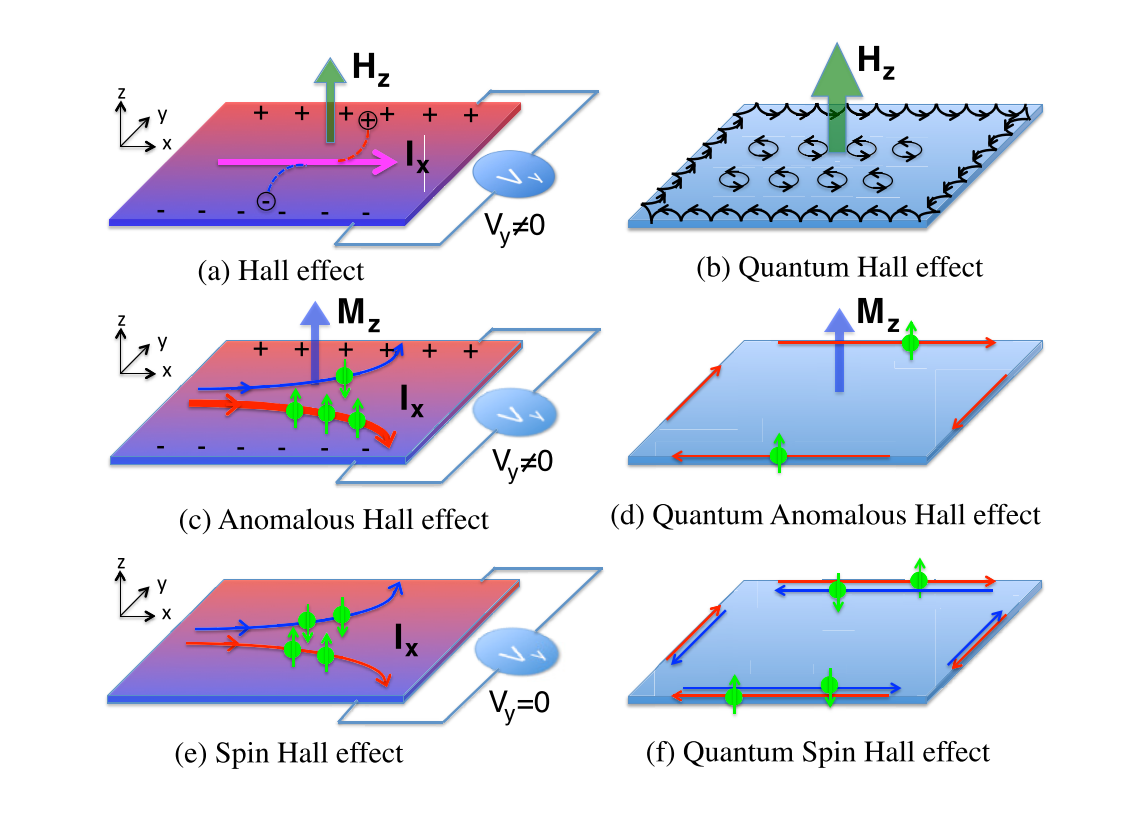
\includegraphics[width=10 cm]{chapter1-1.png}
    \bicaption{(a)霍尔效应。(b)量子霍尔效应。(c)反常霍尔效应。(d)量子反常霍尔效应。(e)自旋霍尔效应。(f)量子自旋霍尔效应。(图片来自\citep{review-arxiv})}
    {(a) Hall effect.  (b) Quantum Hall effect. (c) Anomalous Hall effect. (d) Quantum Anomalous Hall effect.  (e) Spin Hall effect. (f) Quantum Spin Hall effect. (From \cite{review-arxiv})}
    \label{fig:1-1}
\end{figure}

\section{量子霍尔效应}
1980年,Klaus von Klitzing 发现~\citep{Klitzing1980},在非常低的温度下,霍尔电导作为垂直于二维(2D)电子气平面施加的磁场强度的函数,会出现量化的阶梯平台,同时纵向电导为零。这就是著名的量子霍尔效应 (Quantum Hall effect, 简称QHE) 。在量子霍尔效应中,如果对二维体系加一个外磁场$H_z$,电子的回旋运动将形成朗道能级。磁场足够强时,体内的电子将局域在体内做圆周运动,但在边界上因为无法做圆周运动而形成沿着特定方向的边缘运动,如图~\ref{fig:1-1}(b)。而且这些边缘态不会受到杂质的影响。因而载流子的运动是无耗散的,霍尔电导被量化为以$e/h$为单位的量子数$n$,且该量子数$n$与边缘态的数量相对应。后来研究发现,无论是整数还是分数的量子霍尔效应都可以由电子波函数的拓扑性质来解释\citep{Laughlin1981,TKNN1982}。从久保公式得出的霍尔电导里的整数,最初称为TKNN数,其实就是现在被用于表征拓扑不变性的“陈数”(Chern number)。后来,我们把具有非零陈数的二维材料,称为陈绝缘体。所以,陈绝缘体的拓扑分类是$\mathbb{Z}$分类。
\begin{figure}[!htbp]
    \centering
    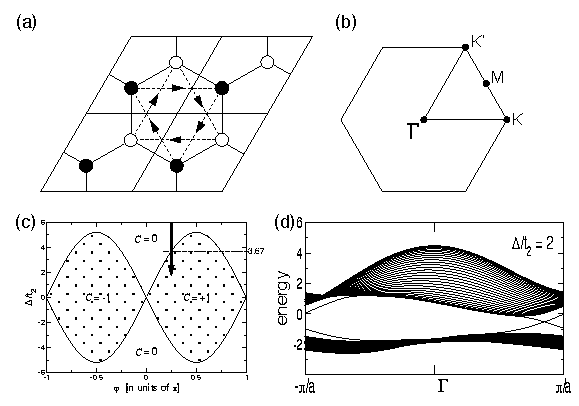
\includegraphics[width=8.5cm]{chapter1-2.pdf}
    \bicaption{(a)Haldane模型的四个原胞。(b)Haldane模型的第一布里渊区。(c)Haldane模型的Chern数,作为参数 $\varphi$ 和 $\Delta/ t_2$ ($t_1=1, t_2=1/3$)的函数。(d)$b_2$方向无限长,而$b_3$方向包含30个原胞的带状格子的能量随波矢$k_y$的变化,$\Delta/t_2 <(\Delta/t_2)_{cr}$。 可以看到手性边界态。(图片来自\citep{Haldane2})}
    {(a) Four unit cells of the Haldane model. (b) First Brillouin zone of the Haldane model. (c) Chern number of the bottom band of the Haldane model as a function of the parameters $\varphi$ and $\Delta/ t_2$ ($t_1=1, t_2=1/3$). (d) Energy vs wave vector $k_y$ for the Haldane model in a
    strip geometry 30 cells wide along the $b_3$ direction and extending infinitely along $b_2$ direction,$\Delta/t_2 <(\Delta/t_2)_{cr}$. Chiral edge states are visible. ( From \cite{Haldane2})}
    \label{fig:1-2}
\end{figure}

第一个超越量子霍尔效应的一个简单的例子是由Haldane在1988年提出的在周期磁场中的石墨烯模型,后称之为Haldane模型\citep{haldane1988model,Haldane2}:
\begin{equation}
    \label{eq:1-2}
    \begin{split}
    \mathbf{H}(\mathbf{k})=&2 t_{2} \cos \phi\left(\sum_{i} \cos \left(\mathbf{k} \cdot \mathbf{b}_{i}\right)\right) \mathbf{I}+t_{1}\left(\sum_{i}\left[\cos \left(\mathbf{k} \cdot \mathbf{a}_{i}\right) \sigma^{1}+\sin \left(\mathbf{k} \cdot \mathbf{a}_{i}\right) \sigma^{2}\right]\right)\\
    &+\left[\Delta-2 t_{2} \sin \phi\left(\sum_{i} \sin \left(\mathbf{k} \cdot \mathbf{b}_{i}\right)\right)\right] \sigma^{3}
    \end{split}
\end{equation}
这个模型如图~\ref{fig:1-2}(a,b),是在二维石墨烯模型的基础上,引入复数的次近邻跃迁(hopping)。$t_{1}$是最近邻不同子格之间的hopping。$t_{2} e^{\pm i \varphi}$就是复数的次近邻hopping(相同子格子之间的hopping)。这个复数hopping的引入使得二维平面有一个周期的磁通,但是体系总磁通仍然为零,这打破了体系原有的时间反演对称性。并且由于A,B子格子的占位能不同(分别为$\Delta,-\Delta$),所以体系不再保持空间反演对称性。
这样一个模型就可以通过改变参数$\varphi, t_2, \Delta$研究普通绝缘体到陈绝缘体的相变\citep{haldane1988model,Haldane2},如图~\ref{fig:1-2} (c) 。当调节参数使得体系进入陈数非零的相时,计算$b_3$方向包含30个原胞的有限厚度的哈密顿量的能带结构,如图~\ref{fig:1-2} (d) ,确实可以在带隙中看到存在两条导电的手性边界态,分别来自左右两个边界。Haldane模型是超越量子霍尔效应之外的拓扑绝缘体的第一个例子。与量子霍尔效应不同的是Haldane模型磁通整体其实是0,也就是说并不需要外加一个磁场就可以实现非平庸的拓扑,即量子反常霍尔效应 (Quantum Anomalous Hall effect, 简称QAHE),如图~\ref{fig:1-1} (d) 。通常把类似于Haldane模型所描述的破坏时间反演对称性且具有非平庸陈数的系统称为陈绝缘体。但是因为这个模型需要手动加入磁通,因而无法在真实材料中实现。
%The Quantum Anomalous Hall Effect has recently been observed in thin films of chromium-doped (Bi,Sb)2Te3 [8].【short review】

\begin{figure}[!t]
    \centering
    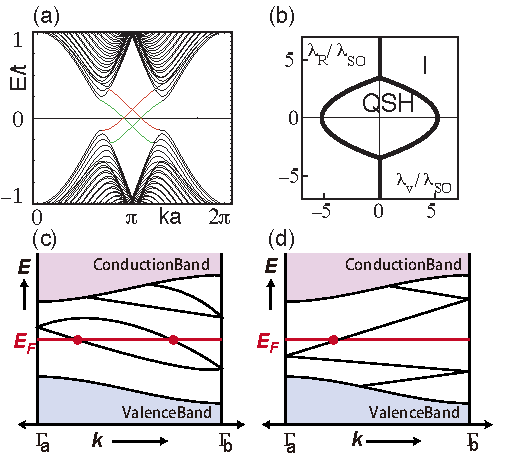
\includegraphics[width=8cm]{chapter1-3.pdf}
    \bicaption{(a)QSH相的一维锯齿形边界能谱。(b)相图,作为以$\lambda_v$ 和 $\lambda_R$ 为变量的函数,$0 < \lambda_{\mathrm{SO}} \ll t$。(c,d)在两个边界克拉默简并点$\Gamma_a=0$和$\Gamma_b=\pi/a$之间的电子色散。在(c)中,表面态穿过费米能$E_F$偶数次,在(d)中,表面态穿过费米能$E_F$奇数次。穿过奇数次的表面态是受拓扑保护的金属边界态。(图片来自\citep{kane2,TIreview,Fu2007topo})}
    { Energy bands for a one-dimensional ‘‘zigzag’’ strip in the (a) QSH phase $\lambda_v=0.1 t$, $\lambda_{SO}=0.06 t$, $\lambda_{R}=0.05 t$. The edge states on a given edge cross at $ka=\pi$. (b)The phase diagram as a function of $\lambda_v$ and $\lambda_R$ for $0 < \lambda_{\mathrm{SO}} \ll t$. (c,d) Electronic dispersion between two boundary Kramers degenerate points $\Gamma_a=0$ and $\Gamma_b=\pi/a$.In (c) the number of surface states crossing the Fermi energy $E_F$ is even, whereas in (d) it is odd. An odd number of crossings leads to topologically protected metallic boundary states. (From~\citep{kane2,TIreview,Fu2007topo})}
    \label{fig:1-3}
\end{figure}

当存在时间反演对称性时,体系的霍尔电导总是为零。那么很自然的就会产生疑问,时间反演对称性是否可以保护非平庸的拓扑呢?换句话说,是否存在时间反演不变的拓扑绝缘体呢?答案是肯定的。那么首先对方程\ref{eq:1-2}做傅立叶变换,Haldane模型在实空间可以写作:
% \begin{equation}
%     \label{eq:1-3}
%     H=t_{1} \sum_{\langle i, j\rangle} c_{i}^{\dagger} c_{j}+t_{2} \sum_{\langle\langle i, j\rangle\rangle} e^{-i \varphi \nu_{ij}} c_{i}^{\dagger} c_{j}+\Delta \sum_{i \in A} c_{i}^{\dagger} c_{i}-\Delta \sum_{i \in B} c_{i}^{\dagger} c_{i}
% \end{equation}

\begin{equation}
    \label{eq:1-3}
    H=t_{1} \sum_{\langle i, j\rangle} c_{i}^{\dagger} c_{j}+t_{2} \sum_{\langle\langle i, j\rangle\rangle} e^{-i \varphi \nu_{ij}} c_{i}^{\dagger} c_{j}+\Delta \sum_{i}\xi_{i} c_{i}^{\dagger} c_{i}
\end{equation}
这里次近邻复数的hopping  $t_2 e^{i\varphi \nu_{ij} }$是由于施加磁场带来的,其中$\nu_{ij}=-\nu_{ji}=\pm 1$取决于最近邻成键的方向。Kane和Mele在Haldane模型的基础上加以修改,认为次近邻之间复数的hopping来自自旋轨道耦合作用\citep{Kane2005,kane2}。Kane-Mele模型可以看作是两个Haldane模型的时间反演版本:
% \begin{equation}
%     \label{eq:1-4}
%     \begin{aligned}
%     H &=t \sum_{\langle i, j\rangle s} c_{i s}^{\dagger} c_{j s}+i \lambda_{\mathrm{so}} \sum_{\langle\langle i, j\rangle\rangle s s^{\prime}} \nu_{i j} c_{i s}^{\dagger} \sigma_{s, s^{\prime}} c_{j s^{\prime}}+i \lambda_{R} \sum_{\langle i, j\rangle s s^{\prime}} c_{i s}^{\dagger}\left(\boldsymbol{\sigma} \times \mathbf{d}_{i j}\right)_{s s^{\prime}}^{z} c_{j s^{\prime}}^{\dagger} \\
%     &+\lambda_{v} \sum_{i \in A, s} c_{i s}^{\dagger} c_{i s}-\lambda_{v} \sum_{i \in B, s} c_{i s}^{\dagger} c_{i s}
%     \end{aligned}
% \end{equation}
\begin{equation}
    \label{eq:1-4}
    \begin{aligned}
    H=& t \sum_{\langle i j\rangle} c_{i}^{\dagger} c_{j}+i \lambda_{\mathrm{SO}} \sum_{\langle\langle i j\rangle\rangle} \nu_{i j} c_{i}^{\dagger} s^{z} c_{j}+i \lambda_{R} \sum_{\langle i j\rangle} c_{i}^{\dagger}\left(\mathbf{s} \times \hat{\mathbf{d}}_{i j}\right)_{z} c_{j}+\lambda_{v} \sum_{i} \xi_{i} c_{i}^{\dagger} c_{i}
    \end{aligned}
\end{equation}
其中$t$相当于$t_1$,$\lambda_{\mathrm{SO}}$相当于$t_2$,是自旋轨道耦合带来的复数hopping。因为每个格点有自旋上、自旋下两个轨道,所以体系仍然有时间反演对称性。$\lambda_{v}$相当于$\Delta$,使得两个子格子占位能占位能不同。$\lambda_{R}= 0$时,自旋上下没有耦合。但是实际体系中往往满足$\lambda_{R}\neq 0$,此时则破坏镜面对称性$M_z$,使得自旋上下的电子之间发生杂化,自旋不再是好的量子数。但是计算发现,此时仍然可以具有拓扑保护的边界态,边界态的数目模2仍然是拓扑不变量,所以其拓扑分类是$\mathbb{Z}_2$分类的\citep{kane2}。这就是我们熟知的QSHE,也称为$\mathbb{Z}_2$拓扑绝缘体,如图~\ref{fig:1-1}(f)。不像量子霍尔效应和量子反常霍尔效应那样,量子自旋霍尔效应的边界导电通道是自旋分辨的,即每个通道只能有一种自旋的电子通过。关于量子自旋霍尔效应的的边缘态是否有很好的弹道输运性质仍然有些争议,但是最近发表在《自然物理》杂志上的一篇文章中,作者证明了由时间反演等反幺正算符保护的边界态是很容易与环境发生耦合的,因而是不稳定的~\citep{2020Fragility},这让我们对这个问题有了一个新的认识。

\section{拓扑绝缘体}\label{sec:system}
在前面的小节,我们已经简单介绍了霍尔效应和它的量子化版本。我们知道了在有时间反演对称性的体系中,也可以有拓扑不平庸的态,即Kane-Mele模型所描述的量子自旋霍尔效应态。然而,这个在石墨烯模型中提出来的理论模型仍然很难在实验上研究,因为在石墨烯中自旋轨道耦合作用非常小,只有$10^{-3}$ meV。随后,斯坦福大学的张首晟等人提出的BHZ模型,预言可以在HgTe/CdTe量子阱中,通过调节量子阱的厚度来研究正常态和量子自旋霍尔态之间的相变,如图~\ref{fig:1-4}(a,b)~\citep{bernevig2004}。
%在基矢$\left|E 1, m_{I}=\frac{1}{2}\right\rangle$,$\left|H 1, m_{I}=\frac{3}{2}\right\rangle$,$\left|E 1, m_{I}=-\frac{1}{2}\right\rangle$和$\left|H 1, m_{I}=-\frac{3}{2}\right\rangle$下,
这个结构的晶格模型可以写作~\citep{bernevig2004,Asboth2015}:
\begin{equation}
    \label{eq:1-5}
    \left.\hat{H}_{\mathrm{BHZ}}(\mathbf{k})=\hat{s}_{0} \otimes\left[\left(u+\cos k_{x}+\cos k_{y}\right) \hat{\sigma}_{z}+\sin k_{y} \hat{\sigma}_{y}\right)\right]+\hat{s}_{z} \otimes \sin k_{x} \hat{\sigma}_{x}+\hat{s}_{x} \otimes \hat{C}
\end{equation}
调节合适的耦合参数C,可以使模型满足时间反演对称性,且$\mathcal{T}^2=-1$。他们发现当HgTe厚度达到临界厚度$d=d_c$时(当模型参数$u=-2$),正常态将到达一个能带反转的态,当HgTe厚度大于临界厚度$d>d_c$,体系进入量子自旋霍尔态。此时可以观察到量子化的霍尔电导。 很快这一理论就被实验所证实~\citep{konig2007quantum},并且在特定厚度的量子阱内观察到量子自旋霍尔边缘态,如图~\ref{fig:1-4}(c)。
\begin{figure}[!t]
    \centering
    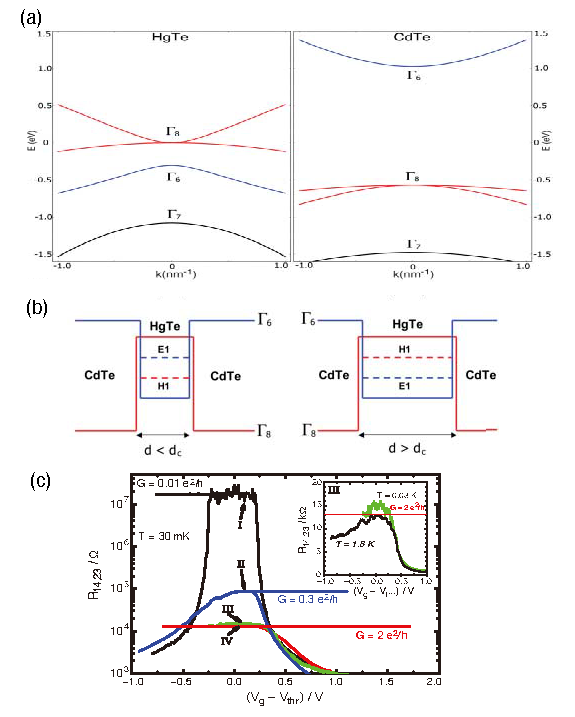
\includegraphics[width=8.5cm]{chapter1-4.pdf}
    \bicaption{(a)HgTe和CdTe在$\Gamma$点附近的体能带图。(b)CdTe-HgTe-CdTe量子阱,在$d < d_c$时E1 > H1,处于正常态。在$d > d_c$时E1 < H1,处于能带反转范围。红色代表$\Gamma_8$表示,蓝色代表$\Gamma_6$表示。(c)纵向四端电阻$R_{14,23}$在不同厚度下随着电压的变化。(图片来自\citep{bernevig2004,konig2007quantum})}
    { (a) Bulk energy bands of HgTe and CdTe near the $\Gamma$ point. (b) The CdTe-HgTe-CdTe quantum well in the normal regime E1> H1 with $d < d_c$ and in the inverted regime H1> E1 with $d > d_c$. $\Gamma_8$/H1 symmetry is indicated in red and $\Gamma_6$/E1 symmetry is indicated in blue. (c) The longitudinal four-terminal resistance, $R_{14,23}$, of various normal (d = 5.5 nm) (I) and inverted (d = 7.3 nm) (II, III, and IV) quantum well structures as a function of the gate voltage measured for B=0 T at T = 30 mK. (From~\citep{bernevig2004,konig2007quantum})}
    \label{fig:1-4}
\end{figure}
所以HgTe/CdTe量子阱是第一个在实验上实现的二维拓扑绝缘体 (Topological insulator,简称TI) 。因为HgTe天然的具有能带反转的特点,BHZ方法的特别之处是利用HgTe这一特点第一次给出了通过调节能带反转来实现非平庸的拓扑,这也为今后对拓扑材料的研究提供了新的思路。但是由于这类材料含毒性元素且热稳定性差,所以在实验制备上带了困难。在2008年, 张首晟研究组又提出一种新的二维拓扑绝缘体材料: AlSb/InAs/GaSb/AlSb 量子阱~\citep{zhang2008,InAs},这类材料也可以实现能带反转,有望在实验上有更广阔的应用。

如上一小节的讨论,时间反演对称性可以保护二维拓扑绝缘体,也称为$\mathbb{Z}_2$拓扑绝缘体。其表面导电模式只能有奇数个,偶数个的表面模式则不能被时间反演保护而打开能隙。这样的量子自旋霍尔态可以通过在二维平面上对占据态的波函数定义一个$\mathbb{Z}_2$不变量来描述。
%这个不变量的详细形式,我们会在后面的小节里仔细讨论。
时间反演保护的拓扑绝缘体还可以扩展到三维(3D)~\citep{Fu2007topo,Fu2007IS}。三维拓扑绝缘体由四个$\mathbb{Z}_2$:$v_0;(v_1,v_2,v_3)$来刻画,$v_0$是一个强拓扑指标,$(v_1,v_2,v_3)$是三个弱拓扑指标,即定义在$k_{x,y,z}=\pi$的面上的$\mathbb{Z}_2$指标。$v_0=0$代表是弱拓扑绝缘体(WTI),$v_0=1$代表强拓扑绝缘体(STI)。弱拓扑绝缘体可以看作是由二维的QSH沿某一个方向堆叠而成,有偶数个表面模但是很容易由杂质破坏,如图~\ref{fig:1-3} (c) 。强拓扑绝缘体则可以看作是由一个QSH和一个拓扑平庸的二维绝缘体交替堆叠而成,有奇数个可以导电的表面态,而且非常稳定,不受弱无序和相互作用的影响 ,如图~\ref{fig:1-3} (d) 。并且不同于二维拓扑绝缘体,三维拓扑绝缘体的表面狄拉克锥除了狄拉克点之外,自旋都是非简并的。在表面狄拉克锥的任意一点自旋动量锁定在一起(spin-momentum locking),如Bi$_2$Se$_3$~\citep{spin2013},由于时间反演和$C_{3v}$对称性,在表面狄拉克锥的任意一个固定的动量$\mathbf{k}$点,哈密顿量形如$\hat{H}=
A (\vec{k} \times \vec{\sigma})$,即自旋总是垂直于动量$\mathbf{k}$,从而
形成独特的螺旋状自旋结构,对于自旋电子学的研究带来了新的途径。

对于有中心反演对称的体系,傅亮和Kane提出了一套简单通过对称性指标就能判断拓扑绝缘体的方法~\citep{Fu2007IS}。并且利用这套方法,2008年,他们首先提出了在$\mathrm{Bi}_{1-x} \mathrm{Sb}_{x}$合金中可以通过掺杂实现三维拓扑绝缘体\citep{fuBiSe},第二年便被角分辨光电子实验所证实\citep{2009hsieh}。这是第一个理论预言并被实验确认的三维拓扑绝缘体。但是因为这个体系的缺点是带隙较小,且是合金,所以表面结构复杂而不易研究。2009年,我们组的方忠、戴希团队提出无需掺杂的层状结构Bi$_2$Se$_3$家族是体态绝缘,表面有狄拉克锥的三维拓扑绝缘体~\citep{zhang2009topological}。Bi$_2$Se$_3$是层状材料,但是层与层之间有一定的相互作用,在考虑自旋轨道耦合时,体能带发生反转且体能隙能达到0.3 eV,有非常强的抗热扰动能力。表面狄拉克点处于费米能附近,且具有非常好的线性色散。这样优质的特点为实验研究提供了非常良好的平台。同年,即被多个实验组所证实~\citep{chen2009experimental,xia2009,hsieh2009}。目前这个家族仍然是作为三维拓扑绝缘体研究最多的材料。顺便提一下,2010年,物理所方忠、戴希团队提出在Bi$_2 $Se$_3$家族中掺Cr,Fe等金属元素可以实现陈绝缘体~\citep{Yu61},随后清华大学薛其坤团队在此体系中第一次观察到量子反常霍尔效应~\citep{xue13},这是Bi$_2 $Se$_3$家族的又一次重大突破。此后,随着人们对拓扑绝缘体的认识越来越深刻,理论计算和实验的手段越来越先进,有越来越多的材料被发现是拓扑绝缘体,包括在三元化合物TlBi$X_2$和TlSb$X_2$($X$=S,Se,Te)系列~\citep{Yan2010,chen10},half-Heusler材料~\citep{half2010}和黄铜矿结构(Chalcopyrite) ~\citep{Feng2011}中发现了很多拓扑绝缘体(其中部分材料我们后来发现其实是外尔半金属,将在第五章详细讨论),还有翁红明、方忠、戴希等发现的准二维大能隙拓扑绝缘体ZrTe$_5$~\citep{wengzrte},还有层状材料ZrSiS家族在考虑自旋轨道耦合时是弱拓扑绝缘体~\citep{xu2015two}等等。

如上所述,凝聚态物理短短几年内在拓扑绝缘体上已经取得了显著的成果,这期间中国物理学者发挥了重要的作用。理论和实验方面相辅相成,结束了对于量子反常霍尔效应20多年的追寻。但是,我们不得不承认这只是在科学史上的一小步,离实际应用还有很大的距离。因为这一次观察量子反常霍尔效应还需要在 100 mK 下的极低温实验室条件里才能实现。所以想要得到应用,就必须要突破在室温下就能实现这一目标。近几年来,随着理论物理学家在磁性理论方面取得的一系列进展~\citep{Watanabe2018,Elcoro2020,xuyf2020,Peng2021},大家开始逐渐将注意力转向不需要掺杂的磁性材料领域,以期在本征的磁性材料内找到量子反常霍尔效应的候选体。
%{\color{red}{ Co3Sn2S2,MnBi2Te4 掀起了这个领域的一个热潮。本论文将在后面的小节里对这几个材料详细介绍}}
2018年,两个团队几乎同时在铁磁外尔半金属Co$_3$Sn$_2$S$_2$中发现了巨反常霍尔效应~\citep{cosns2018,2017Giant}。
相比Cr掺杂的(Bi,Sb)$_2$Te$_3$的铁磁居里温度15K而言,这个材料的居里温度可以达到175K,为高温霍尔效应的研究提供了平台。
另一个明星材料是层状材料MnBi$_2$Te$_4$,它首先被预言为本征的反铁磁拓扑绝缘体~\citep{zhanghj2019,Li2019}。随后实验上又发现奇数层的MnBi$_2$Te$_4$薄膜可以出现净磁矩,甚至可以出现反常霍尔效应~\citep{zhanghj2019,mnbite2,mnbite3,mnbite4,mnbite5}。并且实验上进一步发现在MnBi$_2$Te$_4$中插入Bi$_2$Te$_3$层形成超晶格结构MnBi$_6$Te$_{10}$或者MnBi$_8$Te$_{13}$,使层间反铁磁耦合降低,不需要外场驱动就可以实现净磁矩,从而实现真正的反常霍尔效应~\citep{tian2020,hu2020}。相信这些进展会为实现室温反常霍尔效应提供强有力的动力,也期待这一天早日到来。


\section{拓扑晶体绝缘体}\label{sec:tci}
在前面两个小节的介绍中,我们知道陈绝缘体不受任何对称性保护,其拓扑分类是$\mathbb{Z}$分类。受时间反演对称性保护的绝缘体虽然其陈数总是为零,但是却可以存在$\mathbb{Z}_2$分类,即平庸的偶数类和不平庸的奇数类两类。那么我们就会问,在$\mathbb{Z}_2$为偶数的平庸分类里,是否也存在更加细致丰富的拓扑分类呢?答案是肯定的。当考虑到晶体的对称性时,如旋转对称性,中心反演对称性,镜面对称性等,即使$\mathbb{Z}_2$平庸的一类里,仍然可以存在由其他晶体对称性保护的不平庸拓扑分类,这就是所谓的拓扑晶体绝缘体 (Topological crystalline insulator,简称TCI)。可以说,该领域的发展非常之迅速。2011年,傅亮等人第一次提出拓扑晶体绝缘体的概念~\citep{fu2011topological}。2018年方辰老师团队将第二类磁群保护的拓扑晶体绝缘体完全分类~\citep{song2017}。2021年,方辰老师团队又利用“实空间方法”(real-space recipe)对其他三类磁群对称性保护的拓扑晶体绝缘体做了完整分类~\citep{Peng2021}。从拓扑晶体绝缘体的提出到完全分类只用了10年的时间。在本小节中将根据时间顺序简单梳理一下拓扑晶体绝缘体的发展历史。

\begin{figure}[!htbp]
    \centering
    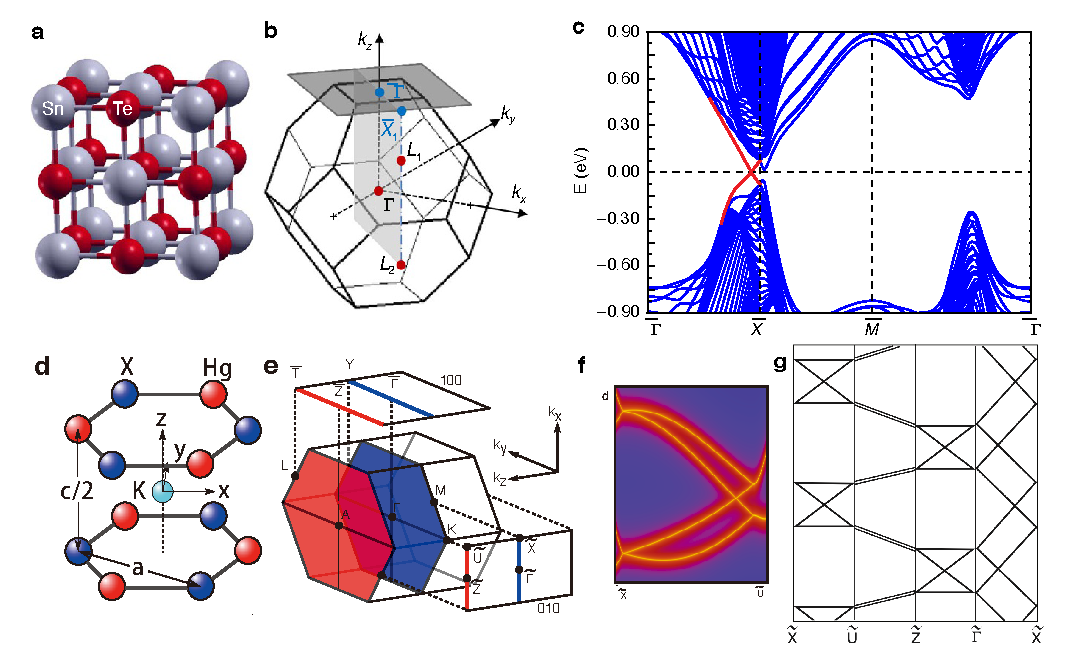
\includegraphics[width=14cm]{chapter1-5.pdf}
    \bicaption{(a)SnTe晶格结构。(b)SnTe的体布里渊区和(001)表面布里渊区。(c)SnTe的(001)表面态。(d)KHg$X$($X$=As, Sb, Bi)的晶体结构。(e)KHg$X$的体布里渊区和(100),(010)表面布里渊区。(f)KHgSb的(010)表面沙漏型色散。(g)不平庸的wilson-loop谱。(图片来自\citep{hsieh2012topological, wang2016hourglass})}
    {(a) SnTe lattice (b) Brillouin zone and [001] surface of SnTe.
    (c) The [001] surface states of SnTe.
    (d) Lattice structure of KHg$X$($X$=As, Sb, Bi).
    (e) bulk Brillouin zone (BZ) of KHg$X$ and 100-surface BZ, 010-surface BZ.
    (f)The dispersion of the hourglass fermion in (010) surface of KHgSb.
    (g)Non-trivial wilson-loop pattern. (From ~\citep{hsieh2012topological, wang2016hourglass})}
    \label{fig:1-5}
\end{figure}
拓扑晶体绝缘体的概念首先由傅亮在2011年提出~\citep{fu2011topological},
他通过紧束缚模型研究了由$C_4$(和$C_6$)旋转对称性加时间反演对称性保护的TCI,并定义了一个新的$\mathbb{Z}_2$不变量。最终发现在保持$C_4$(和$C_6$)不变的(001)表面上,不平庸的$\mathbb{Z}_2$不变量可以保护无能隙的表面态。2012年,傅亮等人又第一次预言了IV–VI族半导体SnTe中可能存在镜面对称性保护的TCI,如图~\ref{fig:1-5} (a-c) , 并且提出PbTe和PbSe经过应力或掺杂后也可以成为TCI~\citep{hsieh2012topological}。同年,角分辨光电子能谱(ARPES)实验很快证实了SnTe和Pb$_{1-x}$Sn$_x$Se中存在由镜面对称性保护的表面狄拉克锥,确实是新型的TCI态~\citep{tanaka2012experimental,Dziawa2012}。这样的体系可以定义的拓扑不变量是镜面陈数。
%,我们会在 (\ref{sec:invariants}) 拓扑不变量这一小节中做详细介绍。

第二个理论预言并在实验上得到验证的是滑移面保护的TCI~\citep{liucx2014,Fang2015new, Shiozaki} -- KHgSb~\citep{wang2016hourglass,ma2017experimental}。这种非简单(non-symmorphic)空间群保护的二维拓扑表面态是一种新奇的沙漏型(hourglass)表面态,如图~\ref{fig:1-5}(d-f),由一个新的$\mathbb{Z}_2$ hourglass拓扑不变量来刻画。由于表面态能谱与Wilson-loop谱是同构的~\citep{fidkowski2011model},也可以计算Wilson-loop谱来判断是否存在不平庸的表面态。如图~\ref{fig:1-5}(g),是表示拓扑不平庸的表面态连接方式,也可以理解为Wilson-loop谱连接方式的示意图。滑移面保护的hourglass表面谱相关性质将在第~\ref{chap:lasbte}章中以LaSbTe为例做更详细的讨论,这里不再赘述。

随后,方辰老师团队又进一步发现了$C_n\mathcal{T}$反常的TCI,在垂直于旋转轴的上下表面分别存在$n$个表面Dirac锥~\citep{songzd2017,Fangc2t},侧表面存在由$C_n$对称性联系起来的棱态,所谓($d-2$)维边界态。其$\mathbb{Z}_2$的拓扑分类可以通过$k_z=0$和$k_z=\pi$面之间瓦尼尔(Wannier)中心的$\mathbb{Z}_2$流来刻画。当然这在实际材料的计算中是很难利用的方法。但是对于同时具有中心反演对称性的体系,可以定义“Fu-Kane-like formula”,直接通过中心反演对称操作的本征值来计算。感兴趣的可以参考原文~\citep{songzd2017,Fangc2t}。后来研究者们也将($d-1$)表面完全开能隙,但是具有($d-2$)维边界态的拓扑晶体绝缘体称为高阶拓扑绝缘体(high-order TI,简称HOTI)~\citep{bernevig17,Schindler,Schindler2018}。2018年,Titus Neupert及其合作者首先预言SnTe经过(110)非轴应力之后可以成为HOTI,即体态和表面态完全开能隙,但是存在由时间反演和镜面对称性保护的螺旋棱态(hinge state)~\citep{Schindler}。同年,他们又理论预言在本征的铋单质(Bismuth,即Bi)中可以出现由空间反演和$C_3$旋转保护的棱态,并通过扫描隧道谱和约瑟夫森干涉实验得到了确凿的实验证据。目前为止,Bi是第一个理论预言并且得到实验验证的高阶拓扑绝缘体~\citep{Schindler2018}。

\begin{figure}[!t]
    \centering
    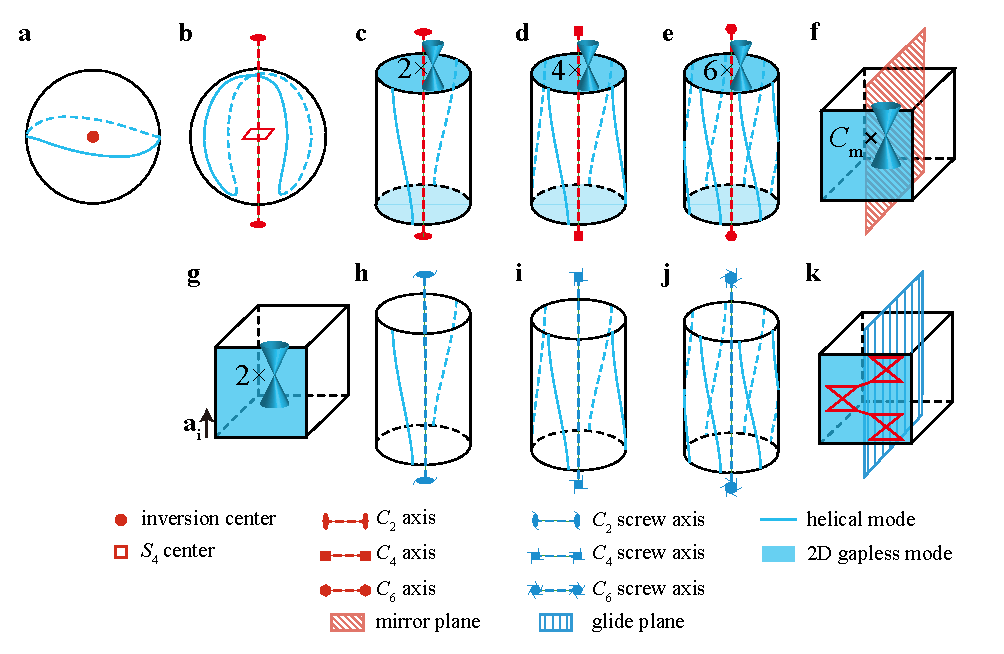
\includegraphics[width=14cm]{chapter1-6.pdf}
    \bicaption{非磁性空间群不同对称性保护的拓扑晶体绝缘体的表面态。由(a)中心反演对称性保护的,(b)S$_4$保护的,(c-e) $C_{n=2,4,6}$旋转对称性保护的,(f)镜面对称性保护的拓扑晶体绝缘体的表面态。(g)弱拓扑绝缘体的表面态。(h-j)$C_{n=2,4,6}$螺旋对称性保护的拓扑晶体绝缘体的表面态。(k)沙漏型的拓扑晶体绝缘体表面态。(图片来自\citep{Song2019})}
    { Surface states of topological crystalline insulators in nonmagnetic space group. The surface state of (a) inversion-protected TCI, (b) S$_4$-protected TCI, (c-e) $C_{n=2,4,6}$-rotation-protected TCI, (f)mirror TCI. (g) The surface state of weak TI. (h-j) The surface states of $C_{n=2,4,6}$-screw-protected TCI. (k) The surface state of hourglass TCI.(From~\citep{Song2019})}
    \label{fig:1-6}
\end{figure}

回顾到此,我们发现镜面对称性,滑移对称性,旋转对称性都可以保护拓扑晶体绝缘体。拓扑晶体绝缘体的完全分类呼之欲出。随着一系列数学物理方法的发展,包括``K-theory",对称性指标理论/拓扑量子化学理论,层构造及实空间构造方法等等,选择一整套可行的方法得到拓扑晶体绝缘体的全部分类似乎是势在必行。2017年底,方辰老师团队首先通过层构造的方法,得到了230个空间群(即第二类磁群)所有的对称性指标和拓扑不变量的映射关系~\citep{song2017}。有了这个映射关系,我们就可以通过简单计算一些对称性指标而获得相对应的可能的拓扑不变量,大大降低了计算的难度。同时这一工作也给出230个空间群中除了
%SG.48, SG.86, SG.134, SG.201 和 SG.224 这五个群是当时用LC方法不能给出所有的indicator。但还有七个群没有indicator,用lc方法不能给出所有的拓扑态。只有用real-space recipe方法之后,才发现这七个态不完整。
Pnn2 (\#34), Pnnn (\#48), P4$_2$ (\#77), P4$_2$/n (\#86), P4$_2$22 (\#93), P4$_2$2$_1$2 (\#94), P4$_2$cm (\#102), P$\bar 4$n2 (\#118), P4$_2$/nnm (\#134), Pn$\bar 3$ (\#201), P4$_2$32 (\#208), 和 Pn$\bar 3$m (\#224)
这12个群之外所有空间群保护的拓扑态~\citep{song2017,Song2019},这使得判断材料具体的拓扑分类成为一件简单的事情。由于非平庸拓扑不变量已经获得,根据体-边对应关系,一定存在不平庸的拓扑表面态。如图~\ref{fig:1-6},显示了不同的拓扑不变量保护的不同表面态构型,包括一些新的拓扑不变量,如螺旋轴不变量保护的螺旋棱态,空间反演对称性和$S_4$不变量保护的棱态。对于层构造方法失效的情况,他们进一步采用局域群保护的拓扑态来替代一个完整二维层构造(2D TI或2D TCI)来装饰每一层(称之为“实空间方法”),最后得到了第二类磁群对称性保护的拓扑晶体绝缘体的全部分类 ~\citep{Song2019}。基于此思想,他们证明了所有由晶体点群对称性保护的拓扑态都可以由更低维度的拓扑态得到,从而给出了拓扑保护的晶体态(包括玻色子和费米子)的完整分类~\citep{Songreal}。
\begin{figure}[!htbp]
    \centering
    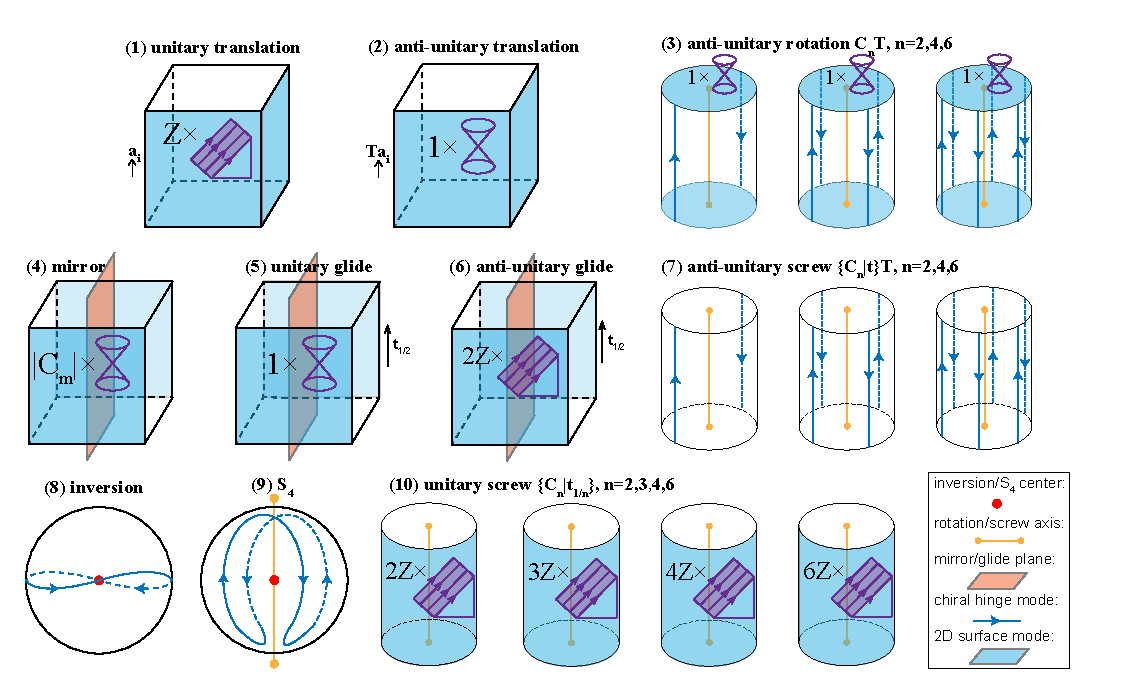
\includegraphics[width=14cm]{chapter1-7.pdf}
    \bicaption{磁空间群的对称操作对应的非平庸拓扑不变量所保护的表面态。二维表面态可以是在(1),(6),(10)中斜坡类型的手性表面态,或者在(2),(3),(4),(5)的狄拉克锥。(图片来自\citep{Peng2021})}
    { Surface states in MSGs, with the corresponding symmetries marked above the plots. The 2D surface modes can be either sloped-like chiral surface modes in (1), (6), (10) or Dirac cones in (2), (3), (4), (5).(From~\citep{Peng2021})}
    \label{fig:1-7}
\end{figure}

2021年年初,方辰老师团队又将“实空间方法”应用到其他三类磁群,给出了每个磁群考虑自旋轨道耦合时的拓扑分类,以及对应的对称性指标和拓扑不变量的映射关系~\citep{Peng2021}。自此完整的分类了所有开能隙的拓扑态。图~\ref{fig:1-7}展示了磁群中不同对称性保护的表面态。除此之外,由于磁群破坏了时间反演对称性,所以会给出一些非磁群不具有的更有意思的结论,比如一些无能隙的拓扑态也可以由不平庸的拓扑不变量来刻画;反幺正的$C_n$旋转对称性给出的表面态是上下只有一个表面狄拉克锥,侧表面的表面态是有$n$个$C_n$对称性联系的手性边界态(chiral hinge mode),而不像非磁性空间群上下表面有$n$个表面狄拉克锥,侧表面有$n$个$C_n$对称性联系的螺旋边界态(helical hinge mode),等等。
相信随着磁性拓扑理论的不断发展~\citep{Elcoro2020,Peng2021},科学家们可以找到更多有意思的材料,如果能够找到一个室温下实现量子反常霍尔效应的材料,必将引领一个新的时代。

\section{拓扑半金属}\label{sec:system}
前面讨论了有能隙的拓扑态,并介绍了这些拓扑态如何进行拓扑分类。那么能否将拓扑分类推广到无能隙的系统呢?我们知道,有能隙的拓扑系统,可以通过占据态的波函数来定义拓扑不变量,因为在布里渊区任意一个$\bold{k}$点,对于绝缘体占据态波函数都有好的定义。但是对于金属而言,不同$\bold{k}$点占据数不同,原来的定义方法就失效了。但是金属不同$\bold{k}$点占据数不同恰好使得其存在费米面,那么我们就可以很自然的利用费米面及其上的波函数来进行拓扑分类。虽然目前为止我们还没有完整分类金属的方法,但是对于半金属,我们可以对其进行分类。因为对于半金属而言,费米面只有一些孤立点或线,而不是一个面,所以可以看作是一种特殊的“绝缘体”。
本论文中,我们主要针对三维空间中三类基本的拓扑半金属:外尔半金属(Weyl Semimetal,即WSM), 狄拉克半金属 (Dirac Semimetal,即DSM), 节点线半金属(Nodal line Semimetal,即NLSM)展开讨论。

\subsection{外尔半金属}\label{sec:weyl}
在三维空间中,两条非简并的能带交叉点附近的低能有效模型一般遵循外尔方程,因而被称为外尔点 (WP)~\citep{1929weyl}。其低能有效哈密顿量形如:
\begin{equation}
    \label{eq:1-6}
    H(\mathbf{k})= \pm \mathbf{k} \cdot \sigma
\end{equation}
然后,我们可以定义包裹外尔点的费米面上的陈数:
\begin{equation}
    \label{eq:1-7}
    C_{\mathrm{FS}}=\frac{1}{2 \pi} \int_{\mathrm{FS}} \boldsymbol{\Omega}(\mathbf{k}) \cdot \mathrm{d} \mathcal{S}
\end{equation}
其中,$\Omega_{\pm}(\mathbf{k})=\mp \frac{\mathbf{k}}{2|k|^{3}}$是贝利曲率,可以看作动量空间的磁场,那么外尔点就可以理解为动量空间的磁单极子。陈数$C_{\mathrm{FS}}=\pm 1$就对应包裹的外尔点的手性为+1或-1。这是描述外尔点的拓扑不变量。
根据“no-go”定理~\citep{NIELSEN198120,NIELSEN1981173},相反手性的外尔点总是成对出现的,在动量空间总陈数为0。
三维空间中三个泡利矩阵是完备基,所以由方程~\ref{eq:1-6}可以看到,这样一个哈密顿量无法加入任何质量项。微扰只能移动外尔点,但不能把它开能隙,除非将两个相反手性的外尔点移动到一起。所以除了要求动量是好的量子数,即只须要求满足平移对称性外不需要其他任何对称性保护,外尔半金属则可以稳定存在。另外,如果体系有其他对称性时,比如$C_4$,$C_6$旋转或者螺旋对称性,外尔点还可以携带更高手性的电荷,此时垂直于旋转轴的色散也不再是简单的线性色散,而是二次型或者三次型色散~\citep{Fang2012,Tsirkin2017}。
那么在三维体系中如何实现这样两重简并的外尔点呢?我们知道如果时间反演$\mathcal{T}$和空间反演$\mathcal{P}$对称性同时存在时,每条能带两重简并,所以这时候的能带交叉点总是相当于两个外尔点相遇在一起。所以要想得到外尔点,我们必须破坏空间反演对称性$\mathcal{P}$,或者时间反演对称性$\mathcal{T}$中的一个。第一种情况对应于非磁性的外尔半金属,第二种情况则对应于磁性外尔半金属。下面我们将对这两种情况加以讨论。

\begin{figure}[!htbp]
    \centering
    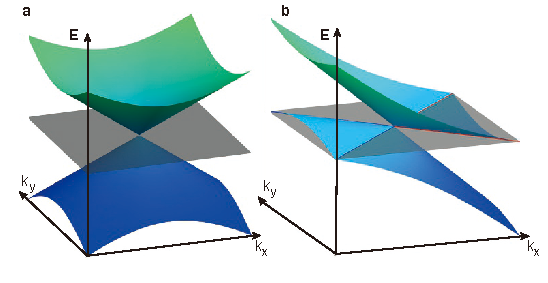
\includegraphics[width=14cm]{chapter1-8.pdf}
    \bicaption{外尔半金属可能的类型。(a)有点状费米面的第一类外尔半金属。(b)出现在电子口袋和空穴口袋接触点的第二类外尔半金属。灰色的面代表费米能级,蓝色(红色)的线代表空穴(电子)口袋的边界。(图片来自\citep{soluyanov2015type})}
    { Possible types of Weyl semimetals. (a) Type-I WP with a pointlike Fermi surface. (b) A type-II WP appears as the contact point between electron and hole pockets. The grey plane corresponds to the position of
    the Fermi level, and the blue (red) lines mark the boundaries of the hole
    (electron) pockets.(From~\citep{soluyanov2015type})}
    \label{fig:1-8}
\end{figure}

对于非磁性外尔半金属,体系内外尔点的数目总是4的倍数。因为如果在动量$\mathbf{k}$处存在一个外尔点,那么由于时间反演对称性使得在动量$-\mathbf{k}$处也存在一个相同手性的外尔点。根据体系中总的外尔点陈数为0,可以知道,一定有另外两个手性相反的外尔点同时存在。非磁性外尔半金属可以看作是拓扑绝缘体到普通绝缘体的相变点~\citep{Murakami_2007,Murakami2}。因为从拓扑绝缘体到普通绝缘体的相变的过程中一定要发生能带反转,而且能带反转前后,占据态的中心反演本征值发生改变,才能带来拓扑的不同~\citep{Fu2007IS},所以能带反转过程中出现的交叉点一定具有不同的中心反演本征值而保证能隙不被打开。这个交叉点就是外尔点。
根据形成外尔点的两条能带的费米速度不同,我们可以将外尔半点分为两种类型,Type I 和Type II~\citep{soluyanov2015type} 。如方程~\ref{eq:1-6}, 一般情况下是点状费米面,如图~\ref{fig:1-8} (a) 所示,我们称这种外尔点是Type I 外尔点。著名的TaAs家族即属于这类。但是在实际材料中,也存在外尔点出现电子口袋和空穴口袋的边界上,如图~\ref{fig:1-8} (b) 所示,我们称这种外尔点是Type II 外尔点,如WTe$_2$, MoTe$_2$。虽然费米速度不同,但是Type II外尔半金属也同样如第一类半金属一样,存在特有的费米弧(Fermi arc)表面态,费米弧连接在表面布里渊区的两个外尔点的投影。但是与此同时,又因为费米面附近不同的态密度,使得Type II外尔半金属又具有不同于Type I外尔半金属的一些新奇的物理性质,如由于动量空间的Klein隧道导致的新奇的量子振荡现象,修正的反常霍尔电导等~\citep{soluyanov2015type,Brien2016}。

对于磁性外尔半金属,允许最少出现两个外尔点。因为如果在动量$\mathbf{k}$处存在一个外尔点,那么由于空间反演对称性使得在动量$-\mathbf{k}$处也存在一个相反手性的外尔点,此时两个外尔点即可满足“no-go”定理。对于一个铁磁性外尔半金属,考虑一个玩具模型~\citep{Armitage2018}:
\begin{equation}
    \label{eq:1-8}
    \begin{aligned}
    H(\mathbf{k})=& t_{z}\left(2-\cos k_{x} a-\cos k_{y} a+\gamma-\cos k_{z} a\right) \sigma_{z}\\
    &+t_{x}\left(\sin k_{x} a\right) \sigma_{x}+t_{y}\left(\sin k_{y} a\right) \sigma_{y}
    \end{aligned}
\end{equation}
这里假设基矢轨道具有相反的宇称,所以$\mathcal{P}=\sigma_{z}$。当$-1<\gamma<1$时,此时宇称相反的能带发生反转,存在一对外尔点位于$(0,0,\pm k_0)$,其中$\cos(k_0)=\gamma$。此时除了$k_z=\pm k_0$的面之外,布里渊区其他$k_z$平面内没有能带简并点,可以定义陈数$\Omega(k_z)$。计算发现$\Omega(|k_z|> k_0)=0$, $\Omega(|k_z|< k_0)=1$。可见外尔点出现在一系列二维陈绝缘体和普通绝缘体之间。所以外尔半金属可以看作是陈绝缘体的三维“强”拓扑态~\citep{weng2015quantum}。总的霍尔电导计算可得$\sigma_{xy}=\frac{e^2}{\pi h} k_0$。所以在铁磁外尔半金属中也可以期望反常霍尔效应的出现。
当化学势恰好在两个外尔点上时,此时费米面是两个点。随着化学势增大,费米面逐渐增大,体系总的霍尔电导逐渐减小,这因为上面能带对贝利曲率的贡献与下面的能带贡献相互抵消所致。当化学势增大到两条能带完全被占据,总的霍尔电导就被完全抵消为零。所以,理想情况下,我们总是希望化学势恰好穿过费米面~\citep{weng2015quantum,Armitage2018}。

外尔半金属因为包裹外尔点的陈数不为零,根据体-边对应关系,可得外尔半金属也一定存在不平庸的表面态。
表征外尔半金属的一个很重要特点就是在表面态上有连接两个外尔点的费米弧。根据上面讨论可知,外尔半金属可以看作由许多二维陈绝缘体和普通绝缘体的堆叠,而这个费米弧的出现也可以看作是这些陈绝缘体的手性边界态。这一特点可以通过ARPES实验来测量。除此之外,外尔半金属还有许多新奇的可观测效应,如手性反常,负磁阻现象,手性磁效应,弱反局域化等等。

材料方面,2011年,南京大学万贤刚老师团队首先在烧绿石铱酸盐提出第一个磁性外尔半金属~\citep{Wan2011}。同年物理所方忠老师团队,预言在铁磁结构HgCr$_2$Se$_4$中存在拓扑电荷为2的双重外尔点~\citep{xu2011chern}。
但是由于ARPES在磁性材料方面测量困难,2014年底,物理所翁红明老师团队首次提出TaAs家族是空间反演对称性破缺的非磁性外尔半金属~\citep{weng2015weyl},很快便得到实验证实~\citep{lv2015experimental,lv2015observation,lv2015observation2}。几乎同时期,普林斯顿研究团队也预言并实验确认了这个材料是外尔半金属~\citep{huang2015weyl,xu2015discovery,xuSY2015}。由于TaAs在样品制备和实验测量方面的优势,目前为止仍然是研究外尔半金属的明星材料。 最近,科学家们又预言了层状Kagome结构铁磁Co$_3$Sn$_2$S$_2$和层状铁磁MnBi$_2$Te$_4$是铁磁外尔半金属~\citep{cosns2018,xucosns,zhanghj2019,Li2019}。并且Co$_3$Sn$_2$S$_2$被观察到巨大的内秉反常霍尔效应~\citep{cosns2018,2017Giant},成为第一个在实验上确认的磁性外尔半金属,这必将为外尔半金属和反常霍尔效应的发展带来更多新的突破。


\subsection{狄拉克半金属}\label{sec:dirac}
狄拉克半金属是一类其低能激发可以用赝相对论狄拉克费米子描述的相。对于一个同时具有时间反演$\mathcal{T}$和空间反演对称性$\mathcal{P}$的体系,动量空间的每一个点必然具有克拉默简并(Kramers' pair),那么两对外尔点就会重合在一起,形成一个四重简并点。那么描述这样一个具有线性色散的简并点的系统至少需要$4\times4$的哈密顿量:
\begin{equation}
    \label{eq:1-9}
    H(\mathbf{k})=\left[\begin{array}{cc}
    \mathbf{k} \cdot \boldsymbol{\sigma} & 0 \\
    0 & -\mathbf{k} \cdot \boldsymbol{\sigma}
    \end{array}\right]
\end{equation}
满足这个方程的无能隙的交叉点,称之为狄拉克点。因为包裹狄拉克点的费米面上的陈数为0,这个简并点是不受拓扑保护的。
显然,方程~\ref{eq:1-7}很容易通过加入一个质量项打开能隙,所以三维狄拉克点并不稳定。事实上,DSM可以看作是普通拓扑绝缘体到拓扑绝缘体相变过程的临界点。根据Murakami等人的理论~\citep{Murakami_2007,Murakami2},总是可以调节外部参数$m$使得当$m=m_c$时,发生相变。但是从这里也可以看出,一旦$m\neq m_c$,狄拉克点将不复存在。
所以要保证狄拉克点稳定存在,则必须考虑额外的晶体对称性,如$n$度旋转对称性$C_{n=2,3,4,6}$,从而使得狄拉克半金属的相变区间不再是一个点。
%%

\begin{table}[!htbp]\footnotesize
    \centering
    \caption{第一类三维狄拉克半金属。(表格来自~\citep{Yang2014})}
    {Classification of Type I 3D Dirac semimetal. (From~\citep{Yang2014})}
    \label{table:1-1}
    %\resizebox{\textwidth}{15mm}{
    \setlength{\tabcolsep}{0.5mm}{
    \begin{tabular}{c c c c c c c c c c c c c c c}
    \hline
%    \hline
    $C_{n}$ & & $|P|$& &$(u_{A,\uparrow},u_{B,\uparrow})$ & & f($k_{\pm}$, $k_{z}$) & & g($k_{\pm}$, $k_{z}$)  & & 2D topological invariant & & $H_{\text{Dirac}}(\textbf{q})$ && Materials\\
    \hline
%    \hline
    $C_{2}$ & & $\tau_{z}$ & & $-$ & & $-$ & & $-$ & & $-$  & & Not allowed & &\\
    $C_{2}$ & & $\tau_{0}$ & & $-$ & & $-$ & & $-$ & & $-$  & & Not allowed & &\\
%    \hline
%    \hline
    $C_{3}$ & & $\tau_{z}$ & &$(e^{i\pi},e^{i\frac{\pi}{3}})$ & & $\beta k_{+}$ & & $\gamma k_{-}$  & & $\nu_{2D}=1$ & & Linear Dirac & & Na$_{3}$Bi\\
    &&&&&&&&&&&&&&~\citep{wang2012dirac} \\
    $C_{3}$ & & $\tau_{0}$ & &$(e^{i\pi},e^{i\frac{\pi}{3}})$ & & $\beta k_{z}k_{+}+\gamma k_{-}^{2}$ & & $\eta k_{z}k_{-}+\xi k_{+}^{2}$  & &$\nu_{2D}=0$ & & Linear Dirac& &\\
%    \hline
%    \hline
    $C_{4}$ & & $\tau_{z}$ & &$(e^{i\frac{3\pi}{4}},e^{i\frac{\pi}{4}})$ & & $\eta k_{+}$ & & $\beta k_{z}k_{+}^{2}+\gamma k_{z}k_{-}^{2}$  & & $n_{M}=\pm1$ & & Linear Dirac
    & & Cd$_{3}$As$_{2}$\\
    &&&&&&&&&&&&&&~\citep{wang2013three} \\
    $C_{4}$ & & $\tau_{0}$ & &$(e^{i\frac{3\pi}{4}},e^{i\frac{\pi}{4}})$ & & $\eta k_{z}k_{+}$ & & $\beta k_{+}^{2}+\gamma k_{-}^{2}$  & &
    $n_{M}=2\text{sgn}(|\beta|-|\gamma|)$ & & Linear Dirac & &\\
%    \hline
%    \hline
    $C_{6}$ & & $\tau_{z}$ & &$(e^{i\frac{\pi}{2}},e^{i\frac{\pi}{6}})$ & & $\beta k_{+}$ & & $\gamma k_{z}k_{+}^{2}$ & & $n_{M}=\pm1$ & & Linear Dirac & &\\
    $C_{6}$ & & $\tau_{0}$ & &$(e^{i\frac{\pi}{2}},e^{i\frac{\pi}{6}})$ & & $\beta k_{z}k_{+}$ & & $\gamma k_{+}^{2}$ & & $n_{M}=\pm2$ & & Linear Dirac & &\\
%    \hline
    $C_{6}$ & & $\tau_{z}$ & &$(e^{i\frac{5\pi}{6}},e^{i\frac{\pi}{2}})$ & & $\beta k_{+}$ & & $\gamma k_{z}k_{-}^{2}$ & & $n_{M}=\pm1$ & & Linear Dirac & &\\
    $C_{6}$ & & $\tau_{0}$ & &$(e^{i\frac{5\pi}{6}},e^{i\frac{\pi}{2}})$ & & $\beta k_{z}k_{+}$ & & $\gamma k_{-}^{2}$ & & $n_{M}=\pm2$ & & Linear Dirac & &\\
%    \hline
    $C_{6}$ & & $\tau_{z}$ & &$(e^{i\frac{5\pi}{6}},e^{i\frac{\pi}{6}})$ & & $\eta k_{z}k_{+}^{2}$ & &$\beta k_{+}^{3}+\gamma k_{-}^{3}$ & &
    $n_{M}=3\text{sgn}(|\beta|-|\gamma|$) & & Quadratic Dirac & &\\
    $C_{6}$ & & $\tau_{0}$ & &$(e^{i\frac{5\pi}{6}},e^{i\frac{\pi}{6}})$ & & $\eta k_{+}^{2}$ & &$\beta k_{z}k_{+}^{3}+\gamma k_{z}k_{-}^{3}$ & & $n_{M}=\pm2$
    & & Quadratic Dirac & &\\
%    \hline 
    \hline
    \end{tabular}
    }
\end{table}
%%
%%%%
\begin{table}[!htbp]\small
    \centering
    \caption{第二类三维狄拉克半金属。(表格来自~\citep{Yang2014})}
    {Classification of Type I 3D Dirac semimetal. (From~\citep{Yang2014})}
    \label{table:1-2}
    %\resizebox{\textwidth}{15mm}{
    \setlength{\tabcolsep}{0.5mm}{
    \begin{tabular}{c c c c c c c c c c c c c}
%    \hline
    \hline
    $C_{n}$ & & $|P|$& &$u_{A,\uparrow}$ & & f($k_{\pm}$, $k_{z}$) & & $g_{z}$($k_{\pm}$, $k_{z}$)   & & $H_{\text{Dirac}}(\textbf{q})$ && Material\\
    \hline
%    \hline
    $C_{2}$ & & $\tau_{x}$ & & $e^{i\frac{\pi}{2}}$ & & $k_{z}F_{1}^{(1)}(k_{x,y})-iF_{2}^{(1)}(k_{x,y})$
    & & $\alpha k_{x}+\beta k_{y}$   & & Linear Dirac && Distorted Spinels\\
    &&&&&&&&&&&&~\cite{spinels}\\
%    ccccccccccccc
%    \hline
%    \hline
    $C_{3}$ & & $\tau_{x}$ & &$-$ & & $-$ & & $-$   & & Not allowed &&\\
%    \hline
%    \hline
    $C_{4}$ & & $\tau_{x}$ & &$e^{\pm i\frac{\pi}{4}}$ & & $F_{1}^{(2)}(k_{x,y})-ik_{z}F_{2}^{(2)}(k_{x,y})$
    & & $\alpha k_{\pm}$   & & Linear Dirac&& BiO$_{2}$\\
    &&&&&&&&&&&&~\cite{Young12}\\
%    \hline
%    \hline
    $C_{6}$ & & $\tau_{x}$ & &$e^{\pm i\frac{\pi}{6}}$ & & $k_{z}F_{1}^{(3)}(k_{x,y})
    +iF_{2}^{(3)}(k_{x,y})$ & & $\alpha k_{\pm}$  & & Linear Dirac &&\\
%    \hline
    $C_{6}$ & & $\tau_{x}$ & &$e^{i\frac{3\pi}{6}}$ & & $k_{z}F_{1}^{(3)}(k_{x,y})
    +iF_{2}^{(3)}(k_{x,y})$ & &$F_{3}^{(3)}(k_{x,y})
    +iF_{4}^{(3)}(k_{x,y})$
    & & Cubic Dirac &&\\
    \hline 
    %\hline
    \end{tabular}}
\end{table}
%%%

根据狄拉克点的位置,可以将DSM分为两类~\citep{Yang2014}:
一类是由于能带反转造成的偶然简并点,使得在旋转轴上存在一对狄拉克点的Type I DSM,如Na$_3$Bi~\citep{wang2012dirac},Cd$_3$As$_2$~\citep{wang2013three}。
%, 此时对称操作满足$\{C_n$,$\mathcal{P}\}$=0。
另一类是由于“对称性强制(symmetry-enforced)”而产生的,只在单个时间反演不变点上存在狄拉克点的Type II DSM,如BiO$_2$~\citep{Young12},扭曲尖晶石~\citep{spinels}。
%,此时对称操作满足[$C_n$,$\mathcal{P}$]=0;
对于第一类由于偶然简并造成的DSM相,可以定义拓扑不变量来进行刻画。因为狄拉克点只在旋转轴上存在,我们可以在$k_z=0$的完全开能隙的面内计算$\mathbb{Z}_2$(或者如果$k_z=0$是镜面, 可计算镜面陈数$n_M$)。狄拉克半金属的两种不同的分类分别列在表格~\ref{table:1-1},~\ref{table:1-2}中。
对于具有非平庸拓扑不变量的狄拉克半金属,根据体-边对应关系,则存在不平庸的拓扑表面态~\citep{Yang2014}。




%\clearpage
\subsection{节点线半金属}\label{sec:nlsm}
节线半金属是区别于外尔半金属和狄拉克半金属的另外一类半金属,其能带简并点在动量空间中是一维的线而非单个孤立的点~\citep{burkov2011}。节线半金属可以在二维系统,也可以在三维系统中存在。我们只讨论三维系统的节线半金属。

根据不同的对称性,节线半金属可以做不同的分类。
在不考虑自旋轨道耦合的情况下,有分别由中心反演和时间反演的组合对称性$\mathcal{PT}$,镜面对称性$M$,非简单空间群对称性$\tilde{g}$这三种对称性保护的三类节线半金属~\citep{fang2015nl,Fang2016cpb}。这三类节线半金属都是外尔节线半金属,即简并点两重简并。在同时存在某些对称性的情况下,也可以出现狄拉克节线半金属,即简并点是四重简并。这种非自旋轨道耦合的狄拉克节线半金属只能出现在空间群57,60,61,62,205这五个空间群里,我们不再做详细讨论,感兴趣的可以参考文献~\cite{Li2021,Yu2021}。$\mathcal{PT}$保护的节线半金属的拓扑分类是$\mathbb{Z}_2$的,因为其波函数的一阶和二阶同伦群都是$\mathbb{Z}_2$。最简单的,我们可以考虑一个两带模型:
\begin{equation}
    \label{eq:1-10}
    H_{0}(\mathbf{k})=g_{x}(\mathbf{k}) \sigma_{x}+g_{y}(\mathbf{k}) \sigma_{y}+g_{z}(\mathbf{k}) \sigma_{z}
\end{equation}
其中$\mathcal{PT}=\mathcal{K}$, $\mathcal{K}$是复共轭算符, 所以$g_{y}=0$。简并点由$g_{x}=g_{z}=0$决定。两个方程,三个未知数,所以解在三维空间中一定是一维的线。当把系统加倍$H_{d}=H_{0}(\mathbf{k}) \oplus H_{0}(\mathbf{k})=s_{0} \otimes H_{0}(\mathbf{k})$,我们发现可以加入一个保持$\mathcal{PT}$对称性的质量项$m s_{y} \sigma_{y}$来打开能隙,这就说明这个节线半金属是$\mathbb{Z}_2$分类的。此时可以定义一个穿过节线半金属的闭环,如图~\ref{fig:1-9} (a) ,计算环绕闭环一周的贝利相位,这个贝利相位就是这类节线半金属的$\mathbb{Z}_2$不变量~\citep{kim2015nl}。这类节线半金属可以通过调节参数使得其收缩为一点,最终完全消失,如图~\ref{fig:1-9} (c) 。
\begin{figure}[!htbp]
    \centering
    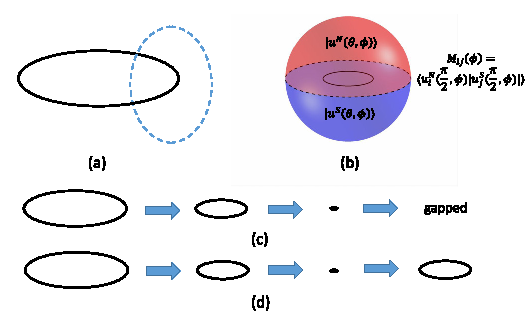
\includegraphics[width=10cm]{chapter1-9.pdf}
    \bicaption{(a)不平庸$\mathbb{Z}_2$不变量:贝利相位$\pi$。(b)对于拓扑不变量定义在球面的节线半金属的2维$\mathbb{Z}_2$不变量。(c)由方程(1.10)描述的零单极电荷的节线半金属的演化。(d)由方程(1.11)描述的有单极电荷的节线半金属随着参数调节的演化。(图片来自\citep{fang2015nl})}
    { (a) A nontrivial $\mathbb{Z}_2$ invariant (Berry’s phase of π) of any loop in 3D BZ implies a nodal line (solid line) passing through the loop. (b) The 2D $\mathbb{Z}_2$ invariant for a nodal line in 3D BZ defined on a sphere enclosing the line. (c) The evolution of a nodal line with zero monopole charge as the parameter changes in the model of Eq. (1.10). (d) The evolution of a nodal line with nonzero monopole charge as the parameter changes in the model of Eq. (1.11). (From~\citep{fang2015nl})}
    \label{fig:1-9}
\end{figure}
方辰老师等人还发现,$\mathcal{PT}$对称性还能保护另外一类$\mathbb{Z}_2$类型的节线半金属,其拓扑不变量由定义在包裹该节线半金属的球面上的$\mathbb{Z}_2$数来决定,如图~\ref{fig:1-9} (b) ~\citep{fang2015nl,Fang2016cpb}。描述这样的一种节线半金属的哈密量可以写作:
\begin{equation}
    \label{eq:1-11}
    H_{0}(\mathbf{k})=k_{x} \sigma_{x}+k_{y} \tau_{y} \sigma_{y}+k_{z} \sigma_{z}+m \tau_{x} \sigma_{x}
\end{equation}
这个哈密顿量描述了一个在$k_z=0$面内半径为$\sqrt{|m|}$的节线环。当调节参数$m$从正数变为负数的过程中, 我们发现节线环会先缩为一点,然后又变回一个节线环,而不会消失,如图~\ref{fig:1-9}(d)。这样的节线半金属只能通过与另一个
$\mathbb{Z}_2$荷相同的节线环相遇才能消除掉。如果把两个方程~\ref{eq:1-11}描述的节线环直和起来$H_{d}=s_{0} \otimes H_{0}(\mathbf{k})$,仍然可以找到一个满足$\mathcal{PT}$对称性的质量项$m^{\prime} s_{0} \tau_{x} \sigma_{y}$,使得节线环不能稳定存在。所以这样的节线环仍然是$\mathbb{Z}_2$分类的。$\mathcal{PT}$保护的节线半金属往往在一般位置上,因而不太容易确定。为此,方辰老师团队发展了一套对称性指标理论,可以确定节线半金属的构型和可能的位置,为理解节线半金属成因和寻找节线半金属起到了重要的作用~\citep{song2018nl}。

不同于$\mathcal{PT}$对称性保护的节线半金属,镜面保护的节线半金属是$\mathbb{Z}$的拓扑分类,同样可以利用上面的“质量项”的方法进行分析,感兴趣的读者可以参考~\citep{chiu2014}。~\cite{chiu2014}文章详细讨论了由镜面对称性保护的节线半金属的拓扑分类问题。当镜面对称性与其他对称性,如时间反演,粒子-空穴对称性,手性对称性等,同时出现时,镜面对称性还会将原本“十重类”(“tenfold-class”)丰富到27类不同的拓扑分类。~\cite{chiu2014}文章同时还给出了由镜面对称性相联系的不处于镜面上的节线半金属的分类。

在考虑自旋轨道耦合的情况下,单独由$\mathcal{PT}$对称性则不再能保护节线半金属。因为我们知道,此时由于克拉默对的存在,每条能带在每个$\mathbf{k}$点都是两重简并的。所以必须考虑更多的对称性,从而形成狄拉克节线半金属。这种情况相对复杂,可以参考文献~\cite{fang2015nl,liang2016,chen2016,shao2020,wu2020}。而对于破坏空间反演$\mathcal{P}$或者时间反演$\mathcal{T}$对称性的节线半金属情况则较为简单,此时单独的镜面对称性或者非简单空间群对称性就可以保护外尔节线半金属,其情况与不考虑自旋轨道耦合时相似,比如在考虑自旋轨道耦合时,Pb(Tl)TaSe$_2$就是典型的镜面对称性保护的非中心对称的外尔节线半金属~\citep{TlTaSe,Bian2016}。表格~\ref{table:1-3}给出了一些典型的节线半金属材料的拓扑分类~\citep{Fang2016cpb}。

和其他拓扑态一样,由体-边对应关系,节线半金属中非平庸的拓扑不变量也会保证表面态的出现。不同于外尔半金属只有零维的无能隙点,节线半金属无能隙的点是一维的线,所以其表面态构型也大不相同。节线半金属的表面态是连接所有无能隙交叉点的平带,由于在三维动量空间中形如鼓膜,也称为“鼓膜态”。如果体系中存在额外对称性时,如手性对称性,节线半金属的表面态是零能的鼓膜态。但是一旦施加一个化学势,鼓膜态就不再是严格的零能态,而是会具有一定的色散。这种新奇的表面态的存在也使得节线半金属具有很多新奇的物理性质,如特别的朗道能级和光电导行为\citep{landau,2016Optical}。
%以$\mathcal{PT}$保护的第一类$\mathbb{Z}_2$不平庸的节点环为例,由于节线半金属中无能隙的点是一维的线(或环),所以-“鼓膜态”(drumhead edge states)。

\begin{table}\small
    \centering
    \caption{一些被理论或者实验认为是节线半金属的材料及其分类。(表格来自\citep{Fang2016cpb})}
    {The proposed materials to host nodal lines classified. The DSM, WSM and TI mean the nodal lines evolve into the corresponding topological state when spin-orbit coupling (SOC) is further included. N/A means unknown. Type-A means that the nodal lines are protected by mirror reflection symmetry; type-B means that the nodal lines are protected by space inversion and time-reversal symmetry; type-C means the existence of dirac-nodal lines. (From~\citep{Fang2016cpb})}
    \label{table:1-3}
%    \resizebox{\textwidth}{15mm}{
    \setlength{\tabcolsep}{0.8mm}{    
    \begin{tabular}{c c c}
    \hline
 %   \hline
    Class   & NO SOC  &  +SOC  \\
         \hline
    Type A & TaAs, ZrTe 				& Weyl semimetal \\
                & CaAg$X$ ($X$=P, As) 	& Topological insulators\\
                &						& HgCr$_2$Se$_4$, TlTaSe$_2$, PbTaSe$_2$\\
%         \hline
    Type B 	& CaP$_3$ & Topological insulators \\
            & MTC, BaSn$_2$, BP, IGN, BCO-C$_{16}$	& Topological insulators\\
            & Be and other alkaline-earth metal, Ca$_3$P$_2$ & N/A\\
            &Cu$_3$(Pd, Zn)N, LaN, CaTe	& Dirac semimetals\\
%         \hline
    Type C &  & SrIrO$_3$, Ba$M$$X_3$ ($M$=V, Nb, Ta, $X$=S, Se) \\
         \hline
%         \hline
    \end{tabular}
    }
\end{table}
    
\section{拓扑材料的判别方法}\label{sec:topodiag}
在本章的前几节我们已经介绍了拓扑理论的背景和一些目前为止已经发现的拓扑态。那如何判断一个体系是否具有拓扑,具有什么样的拓扑呢?最近的拓扑量子化学方法/对称性指标理论和实空间构造的方法的发展就可以很好的解答这两个问题。在本节,我们将简单介绍这几个理论。
%,然后介绍一些常见的拓扑不变量的计算方法。

%脆拓扑,用twisted-boundary conditions~\citep{Song2020}
\subsection{拓扑量子化学和对称性指标理论}
通过元素之间的离子键或共价键描述的绝缘化合物的共同特点是,他们的基态波函数可以绝热地变形为电子局域在原子或原子间的乘积态(局域的瓦尼尔函数)。 这种情况即是拓扑平庸态,称之为原子绝缘体 (atomic insulator, 简称AI) 或者基本能带表示(elementary band representation,简称EBR)。那么,很自然地,如果一个体系占据态的波函数可以等价于一些局域的瓦尼尔函数,那么这个系统就是平庸的。反之,如果存在拓扑阻塞,那么这个系统就是具有拓扑的。这便是拓扑量子化学和对称性指标理论的核心思想~\citep{nc_ashvin,tqc2017}。所谓的AI,就是在实空间的最大Wyckoff位置(maximum Wyckoff position)上放原子轨道,要求所放的原子轨道满足相应Wyckoff位置小群的对称性,由此诱导得到的不等价的表示(的数目)可以构成一个有限的阿贝尔群,我们可以将其记为$\{\textrm{AI}\}$(或EBR)。 针对某个空间群对应的有能隙的系统,我们可以再定义一个群$\{\textrm{BS}\}$,即在满足相容性关系的前提下,由所有占据态能带的最大$\mathbf{k}$点上的表示(数目)构成的群。那么判断一个系统是否拓扑,就简化为比较两个群$\{\textrm{AI}\}$,$\{\textrm{BS}\}$之间的关系,在数学上,如果$\{\textrm{AI}\} \le \{\textrm{BS}\}$成立,就等价于计算二者的商群:
\begin{equation}
    \label{eq:1-12}
    X_{\mathrm{BS}} \equiv \frac{\{\mathrm{BS}\}}{\{\mathrm{AI}\}}
\end{equation}
Watanabe团队~\citep{nc_ashvin}发现,在230个空间群,无论是否考虑自旋轨道耦合和时间反演对称性,$\{\textrm{BS}\}$的维度$d_{\mathrm{BS}}$和$\{\textrm{AI}\}$的维度$d_{\mathrm{AI}}$总是满足$d_{\mathrm{BS}}=d_{\mathrm{AI}}$。所以商群总是个有限群:
\begin{equation}
    \label{eq:1-13}
    X_{\mathrm{BS}}=\mathbb{Z}_{s_{1}} \times \mathbb{Z}_{s_{2}} \times \ldots \times \mathbb{Z}_{s_{d_{\mathrm{BS}}}}
\end{equation}
只要$s_{i}>1$,体系就是拓扑的~\citep{nc_ashvin,Po2020}。
基于此,得到所有空间群的有无自旋轨道耦合和时间反演对称性情况下的拓扑分类,如表格~\ref{tab:Spinful_TRX}和表格~\ref{tab:Spinless_TRX}~\citep{nc_ashvin}。
%%%
%%%%%%%%

\begin{table}[h]\small
    \centering
    \caption{考虑时间反演对称性和自旋轨道耦合的系统的对称性指标。(表格来自\citep{nc_ashvin})}
    {\bf Symmetry-based indicators of band topology for systems with time-reversal symmetry and significant spin-orbit coupling. (From~\citep{nc_ashvin})
    \label{tab:Spinful_TRX}}
    \begin{tabular}{c c} \hline 
    $X_{\rm BS}$ & Space groups \\
    \hline
    $\mathbb Z_{2}$  &  81, 82, 111, 112, 113, 114, 115, 116, 117,118\\
     &119, 120, 121, 122, 215, 216, 217, 218, 219, 220\\
%    \hline
    $\mathbb Z_{3}$  &  188, 190\\
%    \hline
    $\mathbb Z_{4}$  &  52, 56, 58, 60, 61, 62, 70, 88, 126, 130, 133, 135, 136, 137, 138,\\
                     &  141, 142, 163, 165, 167, 202, 203, 205, 222, 223, 227, 228, 230\\
%    \hline
    $\mathbb Z_{8}$  &  128, 225, 226\\
%    \hline
    $\mathbb Z_{12}$  &  176, 192, 193, 194\\
%    \hline
    $\mathbb Z_{2} \times \mathbb Z_{4}$  &  14, 15, 48, 50, 53, 54, 55, 57, 59, 63, 64, 66, 68, 71, 72\\
    & 73, 74, 84, 85, 86, 125, 129,131, 132, 134, 147, 148\\
     & 162, 164, 166, 200, 201, 204, 206, 224\\
%    \hline
    $\mathbb Z_{2} \times \mathbb Z_{8}$  &  87, 124, 139, 140, 229\\
%    \hline
    $\mathbb Z_{3} \times \mathbb Z_{3}$  &  174, 187, 189\\
%    \hline
    $\mathbb Z_{4} \times \mathbb Z_{8}$  &  127, 221\\
%    \hline
    $\mathbb Z_{6} \times \mathbb Z_{12}$  &  175, 191\\
%    \hline
    $\mathbb Z_{2} \times \mathbb Z_{2} \times \mathbb Z_{4}$  &  11, 12, 13, 49, 51, 65, 67, 69\\
%    \hline
    $\mathbb Z_{2} \times \mathbb Z_{4} \times \mathbb Z_{8}$  &  83, 123\\
%    \hline
    $\mathbb Z_{2} \times \mathbb Z_{2} \times \mathbb Z_{2} \times \mathbb Z_{4}$  &  2, 10, 47\\
    \hline
%    \hline
    \end{tabular}\\
    \begin{flushleft}
    $X_{\rm BS}$: the quotient group between the group of band structures and atomic insulators.
    \end{flushleft}
\end{table}
    %%%%%%%% 
    %%%%%%%%

\begin{table}[h]
    \centering
    \caption{考虑时间反演对称性和忽略自旋轨道耦合的系统的对称性指标。(表格来自\citep{nc_ashvin})}
    {\bf Symmetry-based indicators of band topology for systems with time-reversal symmetry and negligible spin-orbit coupling. (From~\citep{nc_ashvin})
    \label{tab:Spinless_TRX}}
    \begin{tabular}{c c} \hline 
    $X_{\rm BS}$ & Space groups \\
    \hline
    $\mathbb Z_{2}$  &  3, 11, 14, 27, 37, 48, 49, 50, 52, 53, 54\\
    & 56, 58, 60, 66, 68, 70, 75, 77, 82, 85, 86,\\
    &  88, 103, 124, 128, 130, 162, 163, 164, 165\\
    &  166, 167, 168,171, 172, 176, 184, 192, 201, 203\\
%    \hline
    $\mathbb Z_{2} \times \mathbb Z_{2}$  &  12, 13, 15, 81, 84, 87\\
%    \hline
    $\mathbb Z_{2} \times \mathbb Z_{4}$  &  147, 148\\
%    \hline
    $\mathbb Z_{2} \times \mathbb Z_{2} \times \mathbb Z_{2}$  &  10, 83, 175\\
%    \hline
    $\mathbb Z_{2} \times \mathbb Z_{2} \times \mathbb Z_{2} \times \mathbb Z_{4}$  &  2\\
    \hline
%    \hline
    \end{tabular}\\
    \begin{flushleft}
    $X_{\rm BS}$: the quotient group between the group of band structures and atomic insulators.
    \end{flushleft}
\end{table}
    %%%%%%%%  
%%%

针对某一个具体的材料而言,怎么判断这个材料的拓扑性质呢?第一步,计算材料所有最大Wyckoff位置上的表示,然后收集起来,就构成一个矢量$\mathbf{n}$;第二步,判断$\mathbf{n} \in\{\mathrm{BS}\}$是否成立?如果不成立,则该材料不满足相容性关系,故为(半)金属。如果成立,则进行第三步:判断$\mathbf{n} \in\{\mathrm{AI}\}$是否成立?如果不成立,则说明体系不能由原子绝缘体线性组合,故存在拓扑,反之是平庸的。当然值得注意的是,即使第二步成立,也可能在非高对称点和线上存在无能隙的点,这是对称性指标理论所不能确定的,如著名的外尔半金属TaAs即属于这种情况。前面我们也提到,对于有中心反演和时间反演的体系,一般位置的能带简并点可以通过方辰老师团队提出的一套对称性指标的方法进行判断~\citep{song2018nl}。对于一些具有特殊对称性的半金属,也可以定义一些新的对称性指标来判断,比如我们后面对于有S$_4$对称性的体系,可以通过S$_4$的拓扑不变量和时间反演的$\mathbb{Z}_2$拓扑不变量的不匹配来判断体系存在外尔点~\citep{Qians4},将在第\ref{chap:s4}章详细讨论。特别是对于磁性系统,许多不平庸的拓扑不变量恰恰对应金属相~\citep{tobedone2019,Peng2021}。另外一些拓扑半金属,可能就只能通过计算一些拓扑不变量来进行判断了。
另外,Bernevig研究团队也独立的给出了这样一套判断拓扑的方法~\citep{tqc2017},他们把AI称为EBR,并且将所有空间群推导出来的EBR和相容性关系都放在了\href{https://www.cryst.ehu.es/}{Bilbao}的网站上,非常方便查询。


\subsection{实空间构造方法}
Watanabe研究团队虽然给出了所有空间群对应的对称性指标群~\citep{nc_ashvin},但是并没有给出相应的对称性指标的计算公式和含义。如第\ref{sec:tci}节所讨论的,2017年底,方辰老师团队利用了实空间构造的方法,给出所有空间群对称性指标的计算公式和其含义。
并且得到了230个空间群的对称性指标和拓扑不变量之间的映射关系~\citep{song2017},随后又将其推广到磁群~\citep{Peng2021}。在第\ref{chap:lasbte}章中,我们将利用层构造方法,来理解LaSbTe这个材料的拓扑绝缘体相和拓扑晶体绝缘体相之间的联系和区别,在这里,我们将不再赘述。

这些对称性指标,为第一性原理计算提供了极大的便利,使得高通量计算分析实际材料的拓扑性质成为可能。2019年,物理所方辰老师团队,南京大学万贤刚老师团队和普林斯顿Bernevig团队~\citep{zhang2019,wanxg2019,Vergniory2019}几乎同时设计出一套自动化搜索材料的方法,计算了现有的材料数据库,为已有的非磁性材料贴上了标签。至此,对于非磁性材料的理论和计算取得了里程碑式的成果。相信,随着磁性拓扑理论的发展~\citep{Watanabe2018,Elcoro2020,Peng2021},磁性材料的高通量计算将会是下一个很快被解决的问题~\citep{xuyf2020}。

\section{主要工作和论文结构}\label{sec:structure}
前面,我们简单回顾了拓扑态的发展历史和相关的拓扑理论。在本论文的后面章节中,首先将在第二章介绍这些拓扑态研究所依赖的主要工具,即基于密度泛函理论的第一性原理计算和瓦尼尔函数方法。然后介绍拓扑理论在第一性原理计算中的应用,主要包括三个方面的内容:第\ref{chap:hfrup}章,介绍超导体HfRuP家族中存在的拓扑态,讨论其实验和理论方面取得的进展;第\ref{chap:lasbte}章,介绍层构造在LaSbTe这个材料的应用,介绍如何利用层构造方法理解LaSbTe拓扑绝缘体和拓扑晶体绝缘体这两个相之间的联系和区别;第\ref{chap:s4}章,介绍在具有S$_4$对称性的系统中如何通过对称性指标判断外尔半金属相;第\ref{chap:summary}章,对整个论文做一个简单的总结。



% 前两章,我们简单回顾了拓扑理论和第一性原理计算的相关理论。在本论文的后面章节中,将介绍拓扑理论在第一性原理计算中的应用,主要包括三个方面的内容:第\ref{chap:hfrup}章,介绍超导体HfRuP家族中存在的拓扑态,讨论了其实验和理论方面取得的进展;第\ref{chap:lasbte}章,介绍层构造在LaSbTe这个材料的应用,介绍如何利用层构造方法理解LaSbTe拓扑绝缘体和拓扑晶体绝缘体这两个相之间的联系和区别;第\ref{chap:s4}章,介绍在具有S$_4$对称性的系统中如何通过对称性指标判断外尔半金属相;第\ref{chap:summary}章,对整个论文做一简单总结。
% \subsection{拓扑不变量}\label{sec:invariants}
% 对于有中心反演对称性的体系,z2很容易通过8个trim点parity来计算。但是对于非中心反演对称性体系,需要用wilsonloop的方法。

%\section{一些新兴的明星拓扑材料}
%\href{https://mp.weixin.qq.com/s/r3VrXf35zjN72j6Tg14SdQ}{MnBi2Te4}
%Co3Sn2S2,EuInAs





\chapter{第一性原理计算及相关理论}\label{chap:first}
在过去的十到二十年间,计算物理已经发展成为一门独立的学科,与理论物理和实验物理呈“三足鼎立”之势。计算物理已经在包括生物学、化学、天体物理学、加速器物理学、固体物理学等诸多领域发挥着重要的作用。在凝聚态领域中,计算物理实际上是一门通过数值方法求解固体中原子分子特性的学科。其关键是表征物质的电子结构信息,即能带结构。
电子能带理论是基于量子力学和统计力学的理论方法。而密度泛函理论则是凝聚态物理中计算电子能带结构的主要理论基础。密度泛函理论的发展使计算物理能够成为连接理论和实验的桥梁,使得计算物理学家能够先于理论和实验物理准确预测一些材料可能的物性,并为实验物理提供研究的平台。基于密度泛函理论发展起来的第一性原理计算(First-Principles calculations),也称为从头计算($\textit{ab initio}$ calculations)的方法,仅需要知道所研究材料的基本信息,如原子结构和组分信息,不需要引入额外的经验参数,就可以使用现有的软件包求解出材料的电子结构,输运性质,热力学性质等,极大的推动了材料物理近几年的发展。其中,我们组在拓扑材料方面预言的拓扑绝缘体Bi$_2$Se$_3$,ZrTe$_5$,狄拉克半金属Na$_3$Bi,Cd$_3$As$_2$,外尔半金属TaAs和节线半金属ZrSiS都先于实验,并迅速将拓扑领域的研究推向高潮。
我们知道第一性原理计算研究离不开软件包的发展,目前成熟的第一性原理软件包有VASP,Wien2K,Openmx,Quantum Espresso,BSDATE等。

瓦尼尔函数方法是在第一性原理计算基础上发展出来的一套数值计算方法,将倒空间的布洛赫函数转化到实空间的瓦尼尔函数,利用实空间哈密顿量进行一系列计算。这个方法的优势是计算量小,速度快,尤其对于处理表面态的性质非常方便,因此也成为目前与第一性原理计算相辅相成的一个非常流行的工具。本章将首先介绍密度泛函理论的发展过程,然后能带理论的重要定理布洛赫定理,最后介绍瓦尼尔函数的一些基本性质。
%和kp模型一起,构成凝聚态计算物理分析物性的三大工具。本章首先将详细介绍密度泛函理论的发展,仅接着将在第一性原理计算基础上发展出来的一套瓦尼尔(Wannier)函数方法,最后介绍一种解析理解能带性质的$\mathbf{k}\cdot \mathbf{p}$方法。

\section{密度泛函理论}
密度泛函理论(DFT)的基本思想是多体相互作用粒子系统的任何性质都可以看作是基态密度$\rho(\vec{r})$的函数。这个证明最早是由Hohenberge和Kohn及Mermin的工作提出来的~\citep{Hohenberg1964,Mermin65}。Kohn-Sham设想将一个多体相互作用的问题用一个自由粒子问题加上考虑多体效应的交换关联函数来代替。下面我们将从描述多粒子体系的哈密顿量出发,一步步介绍如何推导得到DFT理论的基本方程(Kohn-Sham方程) 。 

我们从电子和原子核满足的基本哈密顿量出发,
\begin{equation}
    \label{eq:2-1}
    \begin{aligned}
    \hat{H}&=\hat{H}_e+\hat{H}_N+\hat{H}_{eN}\\
    &=-\frac{\hbar^{2}}{2 m_{e}} \sum_{i} \nabla_{i}^{2}+\frac{1}{2} \sum_{i \neq j} \frac{e^{2}}{\left|\mathbf{r}_{i}-\mathbf{r}_{j}\right|} \\
    &-\sum_{I} \frac{\hbar^{2}}{2 M_{I}} \nabla_{I}^{2}+\frac{1}{2} \sum_{I \neq J} \frac{Z_{I} Z_{J} e^{2}}{\left|\mathbf{R}_{I}-\mathbf{R}_{J}\right|}+\sum_{i, I} \frac{Z_{I} e^{2}}{\left|\mathbf{r}_{i}-\mathbf{R}_{I}\right|}
    \end{aligned}
\end{equation}
上式子由三部分组成,分别为体系中电子,原子核及电子与原子核相互作用三部分。其中,电子部分又分为电子的动能项和电子-电子的相互作用,原子核部分分为原子核的动能项和原子核-原子核的相互作用。这是一个描述多体相互作用的哈密顿量。在实际体系中,每立方米对$i$和$j$的求和是$10^{29}$次方,以当前计算机的算力,是根本无法计算的。因此很有必要通过近似和简化,将其推广到自由粒子的方法。

\subsection{波恩-奥本海默近似}
在方程\ref{eq:2-1}中,直接去掉相互作用项$\hat{H}_{eN}$是不合理的,因为$\hat{H}_{eN}$与其他两项是同一量级的。而整个哈密顿量中唯一可以看作小量的是$\frac{1}{M_I}$。如果将关于核的质量这一项看作是无限小量,那么核的动能项就可以忽略\citep{martin_2004}。这个近似相当于认为原子核只在平衡位置附近振动,而电子则绝热地围绕原子核做高速运动。那么哈密顿量就可以分成两部分考虑,认为考虑电子运动时,原子核在其瞬时平衡位置上,而考虑核运动时,高速运动的电子则相当于一个均匀的背景。这就是著名的绝热近似或波恩-奥本海默(Born-Oppenheimer)近似\citep{Born1927},由波恩和奥本海默在1927年提出。这个近似事实上是非常好的近似,成为后来理解金属中的电子输运性质,绝缘体中极化子的形成,某些金属-绝缘体相变,超导体BCS理论的基础\citep{Born1927}。

多粒子哈密顿量(\ref{eq:2-1})满足的薛定谔方程可以写作:
\begin{equation}
    \label{eq:2-2}
    H \Psi(\mathbf{r}, \mathbf{R})=E \Psi(\mathbf{r}, \mathbf{R})
\end{equation}
经过波恩-奥本海默近似后,薛定谔方程(\ref{eq:2-2})的解就可以写成电子部分和原子核部分波函数的直积形式:
\begin{equation}
    \label{eq:2-3}
    \Psi(\mathbf{r}, \mathbf{R})=\chi(\mathbf{R}) \psi(\mathbf{r}, \mathbf{R})
\end{equation}
其中$\chi(\mathbf{R})$描述原子核的运动,原子核如同在势阱中运动;$\psi(\mathbf{r}, \mathbf{R})$描述电子的运动,认为原子核固定在某瞬时位置\citep{solid}。电子部分波函数$\psi(\mathbf{r}, \mathbf{R})$中原子核的瞬时位置$\mathbf{R}$作为参数出现,故在今后的讨论中略去。此时,原子核满足的薛定谔方程为:
\begin{equation}
    \label{eq:2-4}
    \left(\sum_{\alpha} \frac{\mathbf{P}_{\alpha}^{2}}{2 M_{\alpha}}+\frac{1}{2} \sum_{\alpha \neq \beta} v\left(\mathbf{R}_{\alpha}, \mathbf{R}_{\beta}\right)+\sum_{\alpha} v_{e}\left(\mathbf{R}_{\alpha}\right)\right)\chi(\mathbf{R})=E^I \chi(\mathbf{R})
\end{equation}
电子体系满足的薛定谔方程为:
\begin{equation}
    \label{eq:2-5}
    \left(\sum_{i} \frac{\mathbf{p}_{i}^{2}}{2 m_{e}}+\frac{1}{2} \sum_{i \neq j} \frac{e^{2}}{\left|\mathbf{r}_{i}-\mathbf{r}_{j}\right|}+\sum_{i} v\left(\mathbf{r}_{i}\right)\right)\psi(\mathbf{r}, \mathbf{R})=E\psi(\mathbf{r}, \mathbf{R})
\end{equation}
其中$v_{e}\left(\mathbf{R}_{\alpha}\right)$是电子对原子核的平均作用,$v\left(\mathbf{r}_{i}\right)$是原子核对电子的平均作用。固体材料的性质主要由电子决定,所以我们只关心电子满足的薛定谔方程(\ref{eq:2-5})。此时相对于体系的薛定谔方程(\ref{eq:2-2})已经得到了很大的简化。但是,我们可以看到无论是原子核还是电子满足的薛定谔方程都仍然是多体方程,对于实际求解的难度仍然很大。所以,还需要进一步的近似加以简化。

\subsection{哈特利-福特近似}
薛定谔方程(\ref{eq:2-5})的第二项是电子-电子之间的库仑相互作用,这一项的存在为计算带来了很大的难度。如果这一项不存在,即认为电子不受周围电子的束缚,只受到离子势的微扰相互作用,即变为单电子方程,极大的简化了计算。这就是近自由电子近似。但这种近似显然是粗糙的,因为忽略了与其同量级的相互作用。所以近自由电子近似的应用非常有限,只对一些简单金属,如铜,碱金属比较适用,这类材料往往具有球形的费米面。但这个近似对于引入费米面的概念非常重要。

在此基础上,哈特利(Hartree)提出了一种更为严格的处理方法\citep{hartree_1928},即将电子-电子之间复杂的库仑相互作用看作一种平均势。这时,满足电子薛定谔方程(\ref{eq:2-5})的解则可以表达为单个电子波函数的乘积形式,称为Hartree波函数:
\begin{equation}
    \label{eq:2-6}
    \psi(\mathbf{r})=\varphi_{1}\left(\mathbf{r}_{1}\right) \varphi_{2}\left(\mathbf{r}_{2}\right) \varphi_{3}\left(\mathbf{r}_{3}\right) \cdots \varphi_{N}\left(\mathbf{r}_{N}\right)
\end{equation}
这种近似下,取一组正交归一的$\varphi_{i}(\mathbf{r})$,计算能量的期望值$E$。为得到系统能量最小值,将$E$对$\varphi_{i}(\mathbf{r})$做变分,$E_{i}$作为拉格朗日乘子:
\begin{equation}
    \label{eq:2-7}
    \delta\left[E-\sum_{i} E_{i}\left(\left\langle\varphi_{i} \mid \varphi_{i}\right\rangle-1\right)\right]=0
\end{equation}

则得到每个单电子波函数满足单电子方程:
\begin{equation}
    \label{eq:2-8}
    \left(-\frac{\hbar^{2}}{2 m} \nabla^{2}+V(\mathbf{r})+e^{2} \sum_{i \neq i^{\prime}} \int d \mathbf{r}^{\prime} \frac{\left|\varphi_{i^{\prime}}\left(\mathbf{r}^{\prime}\right)\right|^{2}}{\left|\mathbf{r}^{\prime}-\mathbf{r}\right|}\right) \varphi_{i}(\mathbf{r})=E_{i} \varphi_{i}(\mathbf{r})
\end{equation}
第一项是电子动能项,第二项是单电子受到的晶格势,第三项是但电子受到其他电子的平均库仑势。拉格朗日乘子$E_{i}$有单电子能量的含义。可见,Hartree近似中,哈密顿量是严格,而波函数做了平均场近似。由于第三项的平均库仑势是单电子波函数的函数,所以求解这个薛定谔方程需要用自洽求解的方法。这部分详细讨论可参考:\cite{solid}。

电子是费米子,应当满足泡利不相容原理,即每个电子的量子态不同。这一点Hartree近似是满足的。但是Hartree近似忽略了电子之间的交换反对称性,即任意交换了两个位置的电子,应该产生一个负号。为了满足这个条件,福克(Fock)将单电子的波函数写成了Slater行列式的形式~\citep{Slater30,1930fock}:
\begin{equation}
    \label{eq:2-9}
    \psi(\mathbf{q})=\frac{1}{\sqrt{N !}}\left|\begin{array}{cccc}
    \varphi_{1}\left(q_{1}\right) & \varphi_{1}\left(q_{2}\right) & \cdots & \varphi_{1}\left(q_{N}\right) \\
    \varphi_{2}\left(q_{1}\right) & \varphi_{2}\left(q_{2}\right) & \cdots & \varphi_{2}\left(q_{N}\right) \\
    \vdots & \vdots & \ddots & \vdots \\
    \varphi_{N}\left(q_{1}\right) & \varphi_{N}\left(q_{2}\right) & \cdots & \varphi_{N}\left(q_{N}\right)
    \end{array}\right|
\end{equation}
其中,$\varphi_{i}$是位于$q_i$处的$i$个电子的波函数,$q_i$同时包含位置和自旋。这就是Hartree-Fock近似,也称为分子轨道近似或单行列式近似。再按照Hartree近似推导单电子方程相同的方法,对能量的期望值进行变分,就可以得到单电子的满足的Hartree-Fock方程:
\begin{equation}
    \label{eq:2-10}
    \begin{array}{c}
    \left(-\frac{\hbar^{2}}{2 m} \nabla^{2}+V(\mathbf{r})+e^{2} \sum_{i \neq i^{\prime}} \int d \mathbf{r}^{\prime} \frac{\left|\varphi_{i^{\prime}}\left(\mathbf{r}^{\prime}\right)\right|^{2}}{\left|\mathbf{r}^{\prime}-\mathbf{r}\right|}\right) \varphi_{i}(\mathbf{r}) \\
    -e^{2} \sum_{i \neq i^{\prime}, \|} \int d \mathbf{r}^{\prime} \frac{\varphi_{i^{\prime}}^{*}\left(\mathbf{r}^{\prime}\right) \varphi_{i}\left(\mathbf{r}^{\prime}\right)}{\left|\mathbf{r}^{\prime}-\mathbf{r}\right|} \varphi_{i^{\prime}}(\mathbf{r})=E_{i} \varphi_{i}(\mathbf{r})
    \end{array}
\end{equation}
Hartree-Fock方程在各种计算软件中被广泛采用,被认为是现代量子化学的基石。然而Hartree-Fock近似虽然考虑了电子之间的交换相互作用,但是却没有考虑自旋反平行电子的关联相互作用。所以对于关联相互作用比较强的体系,Hartree-Fock近似不再适用。


% \subsection{Koopmans定理}
% 总能量不是单粒子能量的和。

\subsection{托马斯-费米-狄拉克近似}
%\section{Thomas-Fermi-Dirac近似}
托马斯-费米(Thomas-Fermi)近似~\citep{thomas_1927,fermi_1927,dirac_1930}是密度泛函理论基本思想的来源。在1927年Thomas和Fermi最早的工作中,他们将电子的动能项看作是给定点的局域密度的函数,将系统的电子看作是均匀电子气中非相互作用的电子。他们忽略了电子之间的交换和关联作用。
1930年,狄拉克(Dirac)又将这个理论推广到考虑电子交换相互作用的情况~\citep{dirac_1930}。之后又有很多工作将这一理论推广到非均匀体系。尽管托马斯-费米-狄拉克近似很粗糙,不能足够精确的给出能带结构,但是其物理本质正是后来更为精确的密度泛函理论建立的基础。

\subsection{Hohenberg-Kohn定理}
Hohenberg和W.Kohn在研究非均匀电子气理论时提出两个定理\citep{Hohenberg1964},这使得密度泛函理论变为一个精确的多体理论,可以用于任何处于外势$V_{ext}$中相互作用电子的系统。密度泛函理论正是建立在这两个Hohenberg-Kohn定理之上~\citep{Hohenberg1964}:

定理一:不计自旋的全同费米子系统的基态能量是粒子数密度函数$\rho(\mathbf{r})$的唯一泛函。

定理二:能量泛函$E(\rho)$在粒子数不变条件下对正确的粒子数密度函数$\rho(\mathbf{r})$取极小值,并等于基态能量。

定理一的核心内容是说,决定系统基本物理性质的量是粒子数密度函数$\rho(\mathbf{r})$。定理二的核心内容是讲,在粒子数不变条件下能量泛函对于密度函数的变分就得到系统基态的能量$E_{G}[\rho]$。
对于N个电子相互作用的哈密顿量,可以写作:
\begin{equation}
    \label{eq:2-11}
    \begin{aligned}
    \hat{H}&=T+V_{ee}+V_{ext}\\
    &=-\frac{\hbar^{2}}{2 m_{e}} \sum_{i} \nabla_{i}^{2}+\frac{1}{2} \sum_{i \neq j} \frac{e^{2}}{\left|\mathbf{r}_{i}-\mathbf{r}_{j}\right|}+\sum_{i} V_{\mathrm{ext}}\left(\mathbf{r}_{i}\right)
    \end{aligned}
\end{equation}
第一项是动能项,第二项是电子之间的库仑相互作用,第三项是外势。根据定理一,我们首先将基态能量写成电荷密度泛函的形式:
\begin{equation}
    \label{eq:2-12}
    \begin{aligned}
    E(\rho, V) &=\left\langle\psi(\rho)\left|T+V_{e e}+V_{e x t}\right| \psi(\rho)\right\rangle\\
    &=T(\rho)+V_{e e}(\rho)+\int d^{3} \mathbf{r} V_{e x t}(\mathbf{r}) \rho(\mathbf{r}) \\
    &=T(\rho)+\frac{1}{2} \int d^{3} \mathbf{r} d^{3} \mathbf{r}^{\prime} \frac{\rho(\mathbf{r}) \rho\left(\mathbf{r}^{\prime}\right)}{\left|\mathbf{r}-\mathbf{r}^{\prime}\right|}+E_{x c}(\rho)+\int d^{3} \mathbf{r} V_{e x t}(\mathbf{r}) \rho(\mathbf{r}) 
    %\\& \equiv F(\rho)+\int d^{3} \mathbf{r} V_{e x t}(\mathbf{r}) \rho(\mathbf{r})
    \end{aligned}
\end{equation}
然后根据定理二,基态能量可以通过能量泛函对密度函数变分得到,即
\begin{equation}
    \label{eq:2-13}
    \int \mathrm{d} r \delta \rho(\boldsymbol{r})\left[\frac{\delta T[\rho(\boldsymbol{r})]}{\delta \rho(\boldsymbol{r})}+\int \mathrm{d} \boldsymbol{r}^{\prime} \frac{\rho\left(\boldsymbol{r}^{\prime}\right)}{\left|\boldsymbol{r}-\boldsymbol{r}^{\prime}\right|}+\frac{\delta E_{\mathrm{xc}}[\rho(\boldsymbol{r})]}{\delta \rho(\boldsymbol{r})}+V_{ext}(\boldsymbol{r})\right]=0
\end{equation}
上述方程中仍存在三个问题需要解决,就是如何确定$T[\rho]$,$\rho(\boldsymbol{r})$, $E_{\mathrm{xc}}[\rho]$。为了回答前两个问题,我们就必须要介绍著名的Kohn-Sham $\textit{AnSatz}$~\citep{Kohn-Sham,martin_2004}。

\subsection{Kohn-Sham \it{AnSatz}}
W.Kohn和L.J.Sham在1965年提出一个假设,即现在熟知的“Kohn-Sham $\textit{AnSatz}$”:假定非相互作用的“电子”体系与相互作用电子体系有相同的基态电荷密度~\citep{Kohn-Sham,martin_2004}。具体地,即假定未知的动能泛函$T[\rho]$可以由一个自由粒子的动能泛函$T_s[\rho]$来代替,将二者的差别放到复杂的交换关联函数$E_{\mathrm{xc}}[\rho]$中去。这个假设将一个复杂的多体问题转化为一个独立的单电子问题加上一个复杂的交换关联的问题。这意味着可以用处理自由粒子的方法来处理多体问题。
进一步,取
\begin{equation}
    \label{eq:2-14}
    \begin{array}{c}
    \rho(\boldsymbol{r})=\sum\limits_{i=1}^{N}\left|\varphi_{i}(\boldsymbol{r})\right|^{2} \\
    T_{\mathrm{s}}[\rho]=\sum\limits _{i=1}^{N} \int \mathrm{d} r \varphi_{i}^{*}(\boldsymbol{r})\left(-\nabla^{2}\right) \varphi_{i}(\boldsymbol{r})
    \end{array}
\end{equation}
则由方程\ref{eq:2-14}可得到单粒子满足的方程为:
\begin{equation}
    \label{eq:2-15}
    \left(-\frac{\hbar}{2 m} \nabla^{2}+V_{e x t}(\mathbf{r})+e^{2} \int d^{3}\ \mathbf{r}^{\prime} \frac{\rho\left(\mathbf{r}^{\prime}\right)}{\left|\mathbf{r}^{\prime}-\mathbf{r}\right|}+\frac{\delta E_{x c}(\rho)}{\delta \rho}\right) \varphi_{i}(\mathbf{r})=E_{i} \varphi_{i}(\mathbf{r})
\end{equation}
这就是著名的Kohn-Sham(KS)方程。由于这里的$\rho(\boldsymbol{r})$包含
$ \varphi_{i}$,因此需要自洽求解。后来的计算物理发展出很多处理复杂的交换关联函数的方法,包括局域密度近似(Local Density Approximation, LDA)~\citep{lda1,lda2}和广义梯度近似(Generalized Gradient Approximation, GGA)~\citep{gga1,gga2,pbe}。只要确定交换关联泛函的具体形式,就可以严格求解KS方程,从而得到基态能量,波函数以及其他物理量。
\begin{figure}[!t]
    \centering
    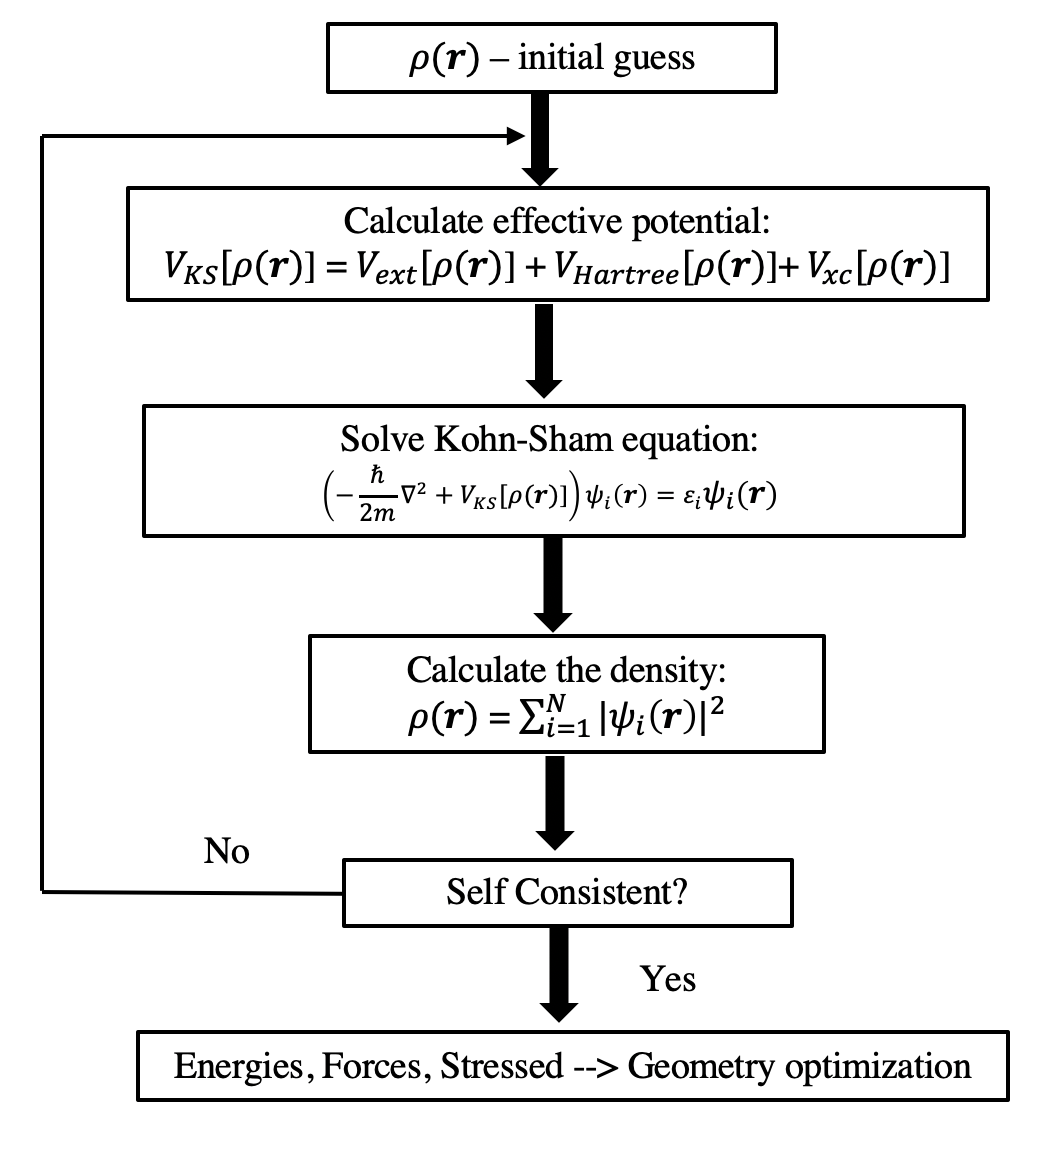
\includegraphics[width=10cm]{chapter2-1.png}
    \bicaption{自洽求解Kohn-Sham方程的流程图。(来自\citep{martin_2004})}{Flow chart of solving the self-consistent Kohn-Sham equation. (From~\citep{martin_2004})}
    \label{fig:2-1}
\end{figure}

自洽求解的流程图如图\ref{fig:2-1},先假设一个初始态密度,利用初始态密度和交换关联函数计算有效势,再带入到KS方程里求解波函数和总能,利用得到的波函数信息计算新的电荷密度,此时检验两个电荷密度是否自洽,如果不自洽就重复上述步骤,直至找到自洽的电荷密度,这样得到的电荷密度,波函数,基态能和其他物理量就是比较准确的。
\section{布洛赫定理及周期场近似}
电子受到的势场包括离子实对电子的势场和电子对电子对平均势场两部分。但是如果把固体看作是理想晶体,那么KS方程中的有效势$V_{eff}=V_{ext}(\mathbf{r})+e^{2} \int d \mathbf{r}^{\prime} \frac{\rho\left(\mathbf{r}^{\prime}\right)}{\left|\mathbf{r}^{\prime}-\mathbf{r}\right|}+V_{xc}(\rho[\mathbf{r})]$具有理想晶体的同样的平移对称性,也就是说它是个严格的周期势场。这个假设称之为周期场近似,或近自由电子近似。布洛赫定理(Bloch theorem)的内容是:

对于周期性势场,即$V(\mathbf{r})=\mathbf{r+R_n}$,其中$\mathbf{R_n}$是布拉维格子任意格矢,则单电子KS方程
\begin{equation}
    \label{eq:2-16}
    H \varphi_{n}(\boldsymbol{r})=\left[-\nabla^{2}+V_{\mathrm{KS}}(\boldsymbol{r})\right] \psi_{n}(\boldsymbol{r})=E_{n} \varphi_{n}(\boldsymbol{r})
\end{equation}
的本征函数是按照布拉维格子周期性调幅的平面波,满足:
\begin{equation}
    \label{eq:2-17}
    \begin{aligned}
    \varphi_{n}(\mathbf{k}, \mathbf{r})&=\mathrm{e}^{i \mathbf{k} \cdot \mathbf{r}} u_{n}(\mathbf{k}, \mathbf{r})\\
    u_{n}(\mathbf{k}, \mathbf{r})&=u_{n}\left(\mathbf{k}, \mathbf{r+R_{n}}\right).
    \end{aligned}
\end{equation}
其中,$\mathbf{k}$的物理意义是倒格矢。根据布洛赫定理,我们可以得到
\begin{equation}
    \label{eq:2-18}
    \begin{aligned}
    \varphi(\mathbf{r+R_{n}})=\mathrm{e}^{i \mathbf{k} \cdot \mathbf{r}} \varphi(\mathbf{r})
    \end{aligned}
\end{equation}
我们通常把满足方程\ref{eq:2-16}和方程\ref{eq:2-17}的函数称为布洛赫波函数。由于倒格矢$\mathbf{k}$具有周期性,所以求解薛定谔方程\ref{eq:2-16}只需要在一个不等价的$\mathbf{k}$区域(第一布里渊区)求解本征值,得到的便是每一个$\mathbf{k}$点给出的一系列分立的能谱$E_n(\mathbf{k})$,称之为能带。只要知道材料的能带信息,波函数信息,就可以进一步分析材料很多基本的物理性质,如拓扑性质、磁有序、光学性质、热导率、振动谱等等。能带理论无疑是凝聚态物理研究的支柱。本论文的工作正是基于固体能带理论来理解材料的拓扑性质。上述部分的详细讨论可以参考文献~\cite{solid,solid2,solid3}。
不同能带计算方法主要分为两类:一类是选择不同的基底展开晶体的布洛赫函数,包括平面波法、正交化平面波方法(orthogonalized plane-wave method, OPW)等;一类是对电子周期势作合理、有效的近似处理,这就是指我们常说的赝势。现在主要有三种赝势方法;模守恒赝势~\citep{Hamann1979,Hamann1989},超软赝势~\citep{soft90}和投影缀加平面波方法~\citep{paw1,paw2}。

\section{瓦尼尔函数}
周期运动的电子的本征函数是布洛赫函数,布洛赫函数是倒空间的周期函数。
%我们可以将布洛赫函数按照实空间基矢展开,展开系数称之为
与布洛赫函数不同,瓦尼尔函数(Wannier function)\citep{Wannier,wf1,wf2}是实空间的一组正交完备的局域函数。所以二者可以通过一个傅立叶变换联系起来。Wannier由于其有非常好的局域性而对于理解材料的电子结构和实际计算带来很大的方便。但是Wannier函数本身又有规范依赖的不确定性,因而为实际使用带来了困难。本节,我们将围绕这个不确定的相因子展开讨论。
% $\varphi_{i}^{\mathbf{k}}(\mathbf{r}) \rightarrow \tilde{\varphi}_{i}^{\mathbf{k}}(\mathbf{r})=\mathrm{e}^{\mathrm{i} \phi_{i}(\mathbf{k})} \varphi_{i}^{\mathbf{k}}(\mathbf{r})$
由布洛赫定理(方程\ref{eq:2-17}),我们知道$\varphi_{n}(\mathbf{k}, \mathbf{r})=\mathrm{e}^{i \mathbf{k} \cdot \mathbf{r}} u_{n}(\mathbf{k}, \mathbf{r})$。当做一个规范变换
$u_{n}^{\mathbf{k}}(\mathbf{r}) \rightarrow \tilde{u}_{n}^{\mathbf{k}}(\mathbf{r})=\mathrm{e}^{\mathrm{i} \phi_{i}(\mathbf{k})} u_{n}^{\mathbf{k}}(\mathbf{r})$,仍然是哈密顿量能量为$E(\mathbf{k})$的本征态。所以,以$\mathbf{R}$为中心的Wannier函数$w_{n\mathbf{R}}(\mathbf{r})$ 可以写作:
\begin{equation}
    \label{eq:2-19}
    w_{n \mathbf{R}}(\mathbf{r})=\frac{V}{(2 \pi)^{3}} \int_{\mathrm{BZ}}\left[\sum_{m} U_{m n}^{(\mathbf{k})} \varphi_{m \mathbf{k}}(\mathbf{r})\right] e^{-\mathrm{i} \mathbf{k} \cdot \mathbf{R}} \mathrm{d} \mathbf{k}
\end{equation}
其中布洛赫函数$U(1)$相因子在多带系统中则是幺正旋转矩阵$U_{m n}^{(\mathbf{k})}$,满足:
\begin{equation}
    \label{eq:2-20}
    u_{n \mathbf{k}}(\mathbf{r}) \rightarrow \sum_{m} U_{m n}(\mathbf{k}) u_{m \mathbf{k}}(\mathbf{r})
\end{equation}
由于$U_{m n}(\mathbf{k})$的不确定性导致Wannier函数的不确定性。那么如何才能得到最局域的Wannier函数呢?

\subsection{最局域的瓦尼尔函数}
为了得到最局域的Wannier函数,则需要最小化$U_{m n}(\mathbf{k})$。为此,定义一个Wannier函数的展宽函数$\Omega$:
\begin{equation}
    \label{eq:2-21}
    \Omega=\sum_{n}\left[\left\langle w_{n 0}(\mathbf{r})\left|r^{2}\right| w_{n 0}(\mathbf{r})\right\rangle-\left|\left\langle w_{n 0}(\mathbf{r})|\mathbf{r}| w_{n 0}(\mathbf{r})\right\rangle\right|^{2}\right]
\end{equation}
展宽函数$\Omega$又可以分为两部分,一部分是规范不变的$\Omega_I$,一部分是依赖于$U_{m n}(\mathbf{k})$的$U_{m n}(\mathbf{k})$的$\tilde{\Omega}$:
\begin{equation}
    \label{eq:2-22}
    \begin{array}{c}
    \Omega=\Omega_{\mathrm{I}}+\tilde{\Omega}=\Omega_{\mathrm{I}}+\Omega_{\mathrm{D}}+\Omega_{\mathrm{OD}} 
    \end{array}
\end{equation}
其中,
\begin{equation}
    \label{eq:2-23}
    \begin{array}{c}
    \Omega_{\mathrm{I}}=\sum\limits_{n}\left[\left\langle w_{n 0}(\mathbf{r})\left|r^{2}\right| w_{n 0}(\mathbf{r})\right\rangle-\sum\limits_{\mathbf{R} m}\left|\left\langle w_{n \mathbf{R}}(\mathbf{r})|\mathbf{r}| w_{n \mathbf{0}}(\mathbf{r})\right\rangle\right|^{2}\right] \\
    \Omega_{\mathrm{D}}=\sum\limits_{n} \sum\limits_{\mathbf{R} \neq 0}\left|\left\langle w_{n \mathbf{R}}(\mathbf{r})|\mathbf{r}| w_{n 0}(\mathbf{r})\right\rangle\right|^{2} \\
    \Omega_{\mathrm{OD}}=\sum\limits_{m \neq n} \sum\limits_{\mathbf{R}}\left|\left\langle w_{m \mathbf{R}}(\mathbf{r})|\mathbf{r}| w_{n 0}(\mathbf{r})\right\rangle\right|^{2}
    \end{array}
\end{equation}
这里$\Omega_D$和$\Omega_{OD}$分别是以Wannier函数为基矢的对角项和非对角项。
计算$\Omega$唯一需要的信息就是交叠矩阵:
\begin{equation}
    \label{eq:2-24}
    M_{m n}^{(\mathbf{k}, \mathbf{b})}=\left\langle u_{m \mathbf{k}} \mid u_{n, \mathbf{k}+\mathbf{b}}\right\rangle
\end{equation}
经过离散$k$空间,然后经过仔细推导\citep{wf1},可以得到如下形式:
\begin{equation}
    \label{eq:2-25}
    \Omega_{\mathrm{I}} =\frac{1}{N} \sum_{\mathbf{k}, \mathbf{b}} w_{b}\left(N-\sum_{m n}\left|M_{m n}^{(\mathbf{k}, \mathbf{b})}\right|^{2}\right)=\frac{1}{N} \sum_{\mathbf{k}, \mathbf{b}} w_{b} \operatorname{tr}\left[P^{(\mathbf{k})} Q^{(\mathbf{k}+\mathbf{b})}\right]
\end{equation}
%
\begin{equation}
    \label{eq:2-26}
    \Omega_{\mathrm{OD}}=\frac{1}{N} \sum_{\mathbf{k}, \mathbf{b}} w_{b} \sum_{m \neq n}\left|M_{m n}^{(\mathbf{k}, \mathbf{b})}\right|^{2} 
\end{equation}
%
\begin{equation}
    \label{eq:2-27}
    \Omega_{\mathrm{D}}=\frac{1}{N} \sum_{\mathbf{k}, \mathbf{b}} w_{b} \sum_{n}\left(-\operatorname{Im} (\ln M_{n n}^{(\mathbf{k}, \mathbf{b})})-\mathbf{b} \cdot \overline{\mathbf{r}}_{n}\right)^{2}
\end{equation}
其中$P^{(\mathbf{k})}=\Sigma_{n}\left|u_{n \mathbf{k}}\right\rangle\left\langle u_{n \mathbf{k}}\right|$, $Q^{(\mathbf{k})}=1-P^{(\mathbf{k})}$,能带指标$m,n$取值为$1,2,...,N$。从方程\ref{eq:2-25}显而易见,如果$\mathbf{k}$点和附近的$\mathbf{k+b}$点的波函数的交叠矩阵的平方越大,$\Omega_{\mathrm{I}}$越小。当两个波函数完全重叠时,这一项为零。所以$P^{(\mathbf{k})} Q^{(\mathbf{k}+\mathbf{b})}$代表的意思是$\mathbf{k}$点的子空间$\mathcal{S}$和$\mathbf{k+b}$点的子空间$\mathcal{S(\mathbf{k+b})}$ 子空间之间的“溢出”程度。
因此最小化$\Omega_I$的过程就是从一个由$N_k$条第一性原理计算的能带展开的$N_k$维的希尔伯特空间$\mathcal{F(k)}$中选出一个由$N$条Wannier轨道构成的$N$维子空间$\mathcal{S(\mathbf{k})}$的过程,在这个子空间中电子几乎局域,能带几乎光滑连接。实际计算中采用的方法就是不断迭代进行,直到达到最佳的“全局平滑度”。这个过程相对简单。

为了获得最局域化的Wannier函数,我们需要进一步优化$\tilde{\Omega}$。Marzari和Vanderbilt提出来的SMV算法\citep{wf2}就是最小化规范依赖的$\tilde{\Omega}$这一项。通过最小化$\tilde{\Omega}$,得到幺正变换矩阵$U_{m n}(\mathbf{k})$,满足
\begin{equation}
    \label{eq:2-28}
    u_{n \mathbf{k}}^{W}=\sum_{m=1}^{N_{\mathbf{k}}} U_{m n}(\mathbf{k}) u_{m \mathbf{k}}
\end{equation}
对$u_{n \mathbf{k}}^{W}$做傅立叶变换就可以得到实空间最局域的Wannier函数。同时对倒空间的哈密顿量做这个幺正变换,就得到此时的$H^W_{nm}(\mathbf{k})$。同样地,对$H^W_{nm}(\mathbf{k})$做傅立叶变换就得到实空间的哈密顿量$H^W_{nm}(\mathbf{R})$。$H^W_{nm}(\mathbf{R})$的物理意义就是在实空间基矢下不同轨道之间的跃迁。得到这个实空间哈密顿量的好处是对涉及实空间格子的处理的计算比较方便,比如表面态的计算,slab计算等。并且对哈密顿量进行处理相比于直接通过第一性原理计算的计算量大大降低,需要的计算资源更少,运算速度大大提高。

\subsection{原子轨道瓦尼尔函数}
我们发现在上述优化过程中没有对对称性有任何约束,这样得到的Wannier函数必然是破坏对称性的。这对于有对称性的晶体结构来讲,得到的能带信息就不准确,这对于分析材料的性质带来了困难。有两个思路来避免这个问题。一个思路是将上述得到的哈密顿量再进行后处理,进行强制对称化。具体操作的步骤就是让哈密顿量满足$
D(R) H\left(R^{-1} \mathbf{k}\right) D^{-1}(R)=H(\mathbf{k})
$,强制使两个由对称联系的矩阵元相等。这个方法已经有现成的软件包来做,但有时对于对称性很差的哈密顿量有时得不到理想的结果。

另一个思路就是直接构造满足对称性的Wannier函数。这个思路又包含两条可行的方法。一个方法是在对称性的限制下重新推导$U_{mn}(\mathbf{k})$~\citep{sakuma}。但这个计算过程比较复杂,对于自旋轨道耦合的体系又有收敛问题。第二个方法是直接构造原子轨道的Wannier函数。其实再上一节中,Marzari等优化$\Omega_I$的过程我们没有详细讨论,事实上具体操作步骤是先找到$N$个局域的试探轨道$\phi_n(\mathbf{r})$,然后投影到$N_k$个布洛赫本征态上,
\begin{equation}
    \label{eq:2-29}
    \left|\tilde{\psi}_{n \mathbf{k}}\right\rangle=\sum_{m=1}^{N_{\mathbf{k}}} A_{m n}\left|\psi_{m \mathbf{k}}\right\rangle
\end{equation}
其中$A_{m n}=\left\langle\psi_{m \mathbf{k}} \mid \phi_{n}\right\rangle$是$N_k \times N$维的投影矩阵。此时的$A_{mn}$就作为初始的$U_{mn}$矩阵,即
\begin{equation}
    \label{eq:2-30}
    \left|\psi_{n \mathbf{k}}^{W}\right\rangle=\sum_{m}\left| \psi_{m \mathbf{k}}\right\rangle \left\langle\psi_{m \mathbf{k}}\mid \phi_{n}\right\rangle=\sum_{m} U_{m n}(\mathbf{k})\left| \psi_{m \mathbf{k}}\right\rangle
\end{equation}
最后优化$U_{mn}$矩阵即可,而不再对$\tilde{\Omega}$进行优化。而选择原子轨道的好处是,我们可以限制原子轨道的Wannier函数满足晶体对称性,进而得到满足对称性的Wannier哈密顿量。对于考虑自旋轨道耦合的情况,我们可以分别对自旋上下进行计算,最后再加上自旋轨道耦合矩阵即可。

假设$\mathbf{k}$为简约布里渊区内一点,$\mathbf{k'}$由对称性操作$\hat{P}_{\{R \mid t\}}$与$\mathbf{k}$相联系,即$\mathbf{k'}=R\ \mathbf{k}$。经过仔细推导,我们会发现$\mathbf{k'}$点的交叠矩阵和投影矩阵满足,
\begin{equation}
    \begin{array}{r}
    A_{m n}^{\mathbf{k}}=\left\langle\psi_{m \mathbf{k}} \mid \phi_{\alpha}^{\mu}\right\rangle=\left\langle\hat{P}_{\{R \mid t\}} \psi_{m \mathbf{k}} \mid \hat{P}_{\{R \mid t\}} \phi_{\alpha}^{\mu}\right\rangle=\left\langle\psi_{m R \mathbf{k}} \mid \phi_{R \alpha}^{\mu^{\prime}}\right\rangle e^{-i(R \mathbf{k}) \cdot \mathbf{R}_{0}} \\
    M_{m n}^{\mathbf{k b}}=\left\langle u_{m \mathbf{k}} \mid u_{n \mathbf{k}+\mathbf{b}}\right\rangle=\left\langle\hat{P}_{\{R \mid t\}} e^{-i k \cdot r} \psi_{m \mathbf{k}} \mid \hat{P}_{\{R \mid t\}} e^{-i(k+b) \cdot r} \psi_{n \mathbf{k}+\mathbf{b}}\right\rangle \\
    =\left\langle e^{-i R \mathbf{k} \cdot t} u_{m, R \mathbf{k}} \mid e^{-i R(\mathbf{k}+\mathbf{b}) \cdot t} u_{n, R \mathbf{k}+\mathbf{b}}\right\rangle=M_{m n}^{R \mathbf{k}, R \mathbf{b}} e^{-i R \mathbf{b} \cdot t}
    \end{array}
\end{equation}
这样只要计算简约布里渊区内$\mathbf{k}$点的交叠矩阵$M_{m n}^{\mathbf{k b}}$和投影矩阵$A_{m n}^{\mathbf{k}}$,其他对称性相联系的$\mathbf{k'}$点的情况就可以由上式得到。通过这个方法,不仅可以得到保持对称性的Wannier函数,还可以提高运算速度。
%再通过L$\ddot{o}$wdin对称性正交化过程得到$N$个正交的轨道$\left|{\psi}^0_{n \mathbf{k}}\right\rangle$。最后再将这$N$个布洛赫函数转化为原胞周期函数$u^0_n(k)$


%\section{Wilson-loop方法}
%\section{{$\bold{k}$}\cdot {$\bold{p}$}微扰理论}


\chapter{超导体HfRuP家族中的拓扑态}\label{chap:hfrup}


基于第一性原理计算和实验测量,我们报道了三元相变金属磷化物TT'X (T=Zr, Hf; T'=Ru; X=P, As) 具有拓扑不平庸的性质。这类材料是已知的非中心对称且有较高的转变温度的超导体。在超导转变温度之前,我们发现
HfRuP属于外尔半金属,有12对第II类外尔点;而ZrRuAs,ZrRuP和HfRuAs属于拓扑晶体绝缘体,有平庸的Fu-Kane $\mathbb Z_2$指标,但有非平庸的镜面陈数。这种有两类不同的拓扑态的非中心对称超导体的高质量的单晶样品已经由实验获得,而且超导性也得到实验验证。ZrRuAs比较宽范围的能带结构已经由ARPES确认,并由理论计算重复。与本征的超导性质相结合,这种正常态不平庸的拓扑性可能会在体态和表面态产生非传统的超导性。我们的发现将会激起大量的实验对这类化合物可能的拓扑超导性进行探索。


\section{背景}
    
拓扑绝缘体~\citep{TIreview,qi2011}和拓扑半金属~\citep{Wan2011,xu2011chern,wang2012dirac,wang2013three,weng2015weyl} 由于存在新奇的拓扑态在过去几年受到了极大的关注,例如拓扑绝缘体中自旋-动量锁定的无能隙表面态~\citep{PhysRevLett.106.257004,zhang2013spin}, 和外尔半金属中的负磁阻~\citep{weng2015weyl,huang2015observation,zhang2016signatures}和费米弧态~\citep{xu2016observation,xu2015discovery,wang2016observation2}。这些绝缘体可以由拓扑不变量和拓扑指标来刻画, 如对拓扑绝缘体和拓扑晶体绝缘体分别由Fu-Kane $\mathbb Z_2$ 指标~\citep{Fu2007topo}和镜面陈数~\citep{hsieh2012topological,nie2016band} 来刻画。但是,外尔半金属是有具体的偶然的二度简并点的拓扑金属态,可由三维的外尔方程来描述。由于缺少严格的洛伦兹不变量,第II类外尔半金属会强烈倾斜~\citep{soluyanov2015type},这在高能物理中没有对应。与具有点状体费米面的第I类外尔半金属~\citep{weng2015weyl,huang2015weyl,lv2015experimental,lv2015observation,lv2015observation2,nie2017topological,nie2019magnetic,PhysRevLett.117.236401}相比,第II类外尔半金属~\citep{deng2016experimental,jiang2017signature,tamai2016fermi,liang2016electronic,wang2016mote} 在外尔点既有电子型的口袋,又有空穴型的口袋,这带来了各种各样新奇的物理性质~\citep{kumar2017extremely,shekhar2015extremely}。
    
    
有超导性的拓扑材料是探测拓扑超导(TSC)和马约拉那费米子(Majorana)的理想系统~\citep{yan2013large,wu2015,Schoop2015,chang2016,wang2016spontaneous,xie2017,nie2018}。拓扑狄拉克锥表面态可以与本征的体态超导来诱导产生2D的拓扑超导~\citep{Fu2008superconducting,Fu2010odd,alicea2012new,sato2017topological}。最近,FeTe$_{1-x}$Se$_x$~\citep{wang2015,xu2016}的拓扑表面狄拉克锥态的超导能隙已经由分辨光电子能谱~\citep{Zhang182}和扫描隧道显微镜~\citep{Wang333}实验探测到了。在非中心对称外尔半金属中,3D时间反演对称的拓扑超导可以由具有不同陈数的费米表面中的符号变化的超导性诱导\citep{qi2010,Hosur204}。但是,据我们所知,几乎所有非中心对称的外尔半金属需要外部压力或者掺杂去诱导或者提高超导性\citep{pan2015pressure,kang2015superconductivity,qi2016superconductivity,chen2016superconductivity,li2017concurrence,xu2019topological}。由于缺少合适的候选材料,3D拓扑超导在实验上研究的非常少。因此,高质量的外尔半金属单晶材料的提出和相关的更高的超导转变温度(T$_C$)引起科学家们极大的兴趣。   
    
    
三维相变金属磷化物TT'X (T=Zr, Hf; T'=Ru; X=P, As)是一系列已知的超导体~\citep{barz1980ternary,meisner1983superconductivity}。我们知道,对于这些化合物有三类不同类型的晶体结构\citep{MULLER1983177,meisner1983superconductivity},即Fe$_2$P-类六角结构单晶 (h-相) ,TiNiSi-类正交结构 (o-相) , 和TiFeSi-类正交结构 (o$'$-相) 。在 h- 和 o- 相中发现有超导性,而且一般来说 h- 相的超导转变温度$T_C$比 o- 相更高。在这个工作里,我们仅关注TT'X的 h- 相,这个相表现出相对较高的转变温度$T_C$ (例如,HfRuP的$T_C$为12.7 K \citep{barz1980ternary},ZrRuP为13.3 K,ZrRuAs为12 K \citep{meisner1983superconductivity})。根据第一性原理计算,我们揭示了这些材料在正常状态(T $ _C $以上)的非平庸的拓扑特性。
当忽略自旋轨道耦合(SOC)时,它们在$k_z=0$面内拥有略高于费米能量 (E$_F$) 的两个节点环,每个环在六角布里渊区(BZ)里环绕K点。 在考虑SOC后,他们或者是由于缺少中心反演进入有12对第二类外尔点的外尔半金属相 (例如 HfRuP) , 或者是进入有平庸Fu-Kane $\mathbb Z_2$指标\citep{Fu2007topo}但有非零陈数的拓扑晶体绝缘体相。这些材料中不平庸的电子态
可以激发有关拓扑电子状态与超导性相互作用的大量实验研究的兴趣。
    
    
\section{结果和讨论}
\subsection{计算方法}
本课题采用了基于缀加平面波方法~\citep{paw1,paw2}的VASP软件包 \citep{KRESSE199615,vasp}进行第一性原理计算。采用PBE类型的GGA作为交换关联泛函 \citep{pbe}。平面波截断能设为400 eV。 采用10 $\times$10 $\times$ 16 k网格做自洽计算。采用了实验的晶格常数\citep{Meisner1983,MEISNER1983983}。内部原子位置完全弛豫,直到所有原子受力小于0.01 eV/\AA~[弛豫后的原子位置在表格~\ref{tab:str}]。计算了考虑和不考虑自旋轨道耦合的电子能带结构。拓扑不变量和手性电荷通过Wilson-loop方法计算。采用最局域Wannier函数方法计算了表面态\citep{mlwf}。


\begin{table}[!h]\scriptsize
    \centering
    \bicaption{TT'X的 h- 相(P$\bar 62m$) 化合物的ICSD号,晶格常数($a$和$c$),实验数据和弛豫后的数据。
    三个X原子在原胞中占据1b Wyckoff位置(0, 0, 1/2)和2c Wyckoff 位置(1/3, 2/3, 0)。这里($\alpha,\beta,\gamma$)是以(a, a, c)为单位的分数坐标。~\citep{qian2019npj}
    }
    {The ICSD number, lattice constants ($a$ and $c$), experimental data and relaxed data of the h-phase (P$\bar 62m$) of the TT'X compounds are given. Three X atoms occupy both the 1b Wyckoff (0, 0, 1/2) and the 2c Wyckoff (1/3, 2/3, 0) positions in a unit cell. Here, a fractional position ($\alpha,\beta,\gamma$) is given in units of (a, a, c). ~\citep{qian2019npj}
    }\label{tab:str}
    \begin{tabular} {cccccc}
%    \hline
    \hline
      Compound  & ICSD Number& $a$ (\AA) & $c$ (\AA)  & Experimental data & Relaxed data \\
    \hline
    HfRuP & \#53035\cite{Meisner1983} & 6.414 & 3.753  &  Hf (0.585, 0, 0.5); Ru (0.243, 0, 0) &  Hf ( 0.584, 0, 0.5); Ru (0.245, 0, 0)  \\
%    \hline
    ZrRuP & \#648037\cite{Meisner1983}& 6.459 & 3.778  &  Zr (0.603, 0, 0.5); Ru (0.263, 0, 0) &  Zr ( 0.584, 0, 0.5); Ru (0.243, 0, 0)  \\
%    \hline
    HfRuAs&\#604605\cite{Meisner1983}  &6.568 &3.842   &  Hf (0.584, 0, 0.5); Ru (0.245, 0, 0) &  Hf ( 0.582, 0, 0.5); Ru (0.245, 0, 0)  \\
%    \hline
    ZrRuAs& \#611301\cite{MEISNER1983983} & 6.586 &3.891  &  Zr (0.580, 0, 0.5); Ru (0.250, 0, 0) &  Zr ( 0.582, 0, 0.5); Ru (0.243, 0, 0)  \\
    \hline
%   \hline
    \end{tabular}
\end{table}

\subsection{晶体结构和电子结构}
\begin{figure}[!htbp]
    \centering
    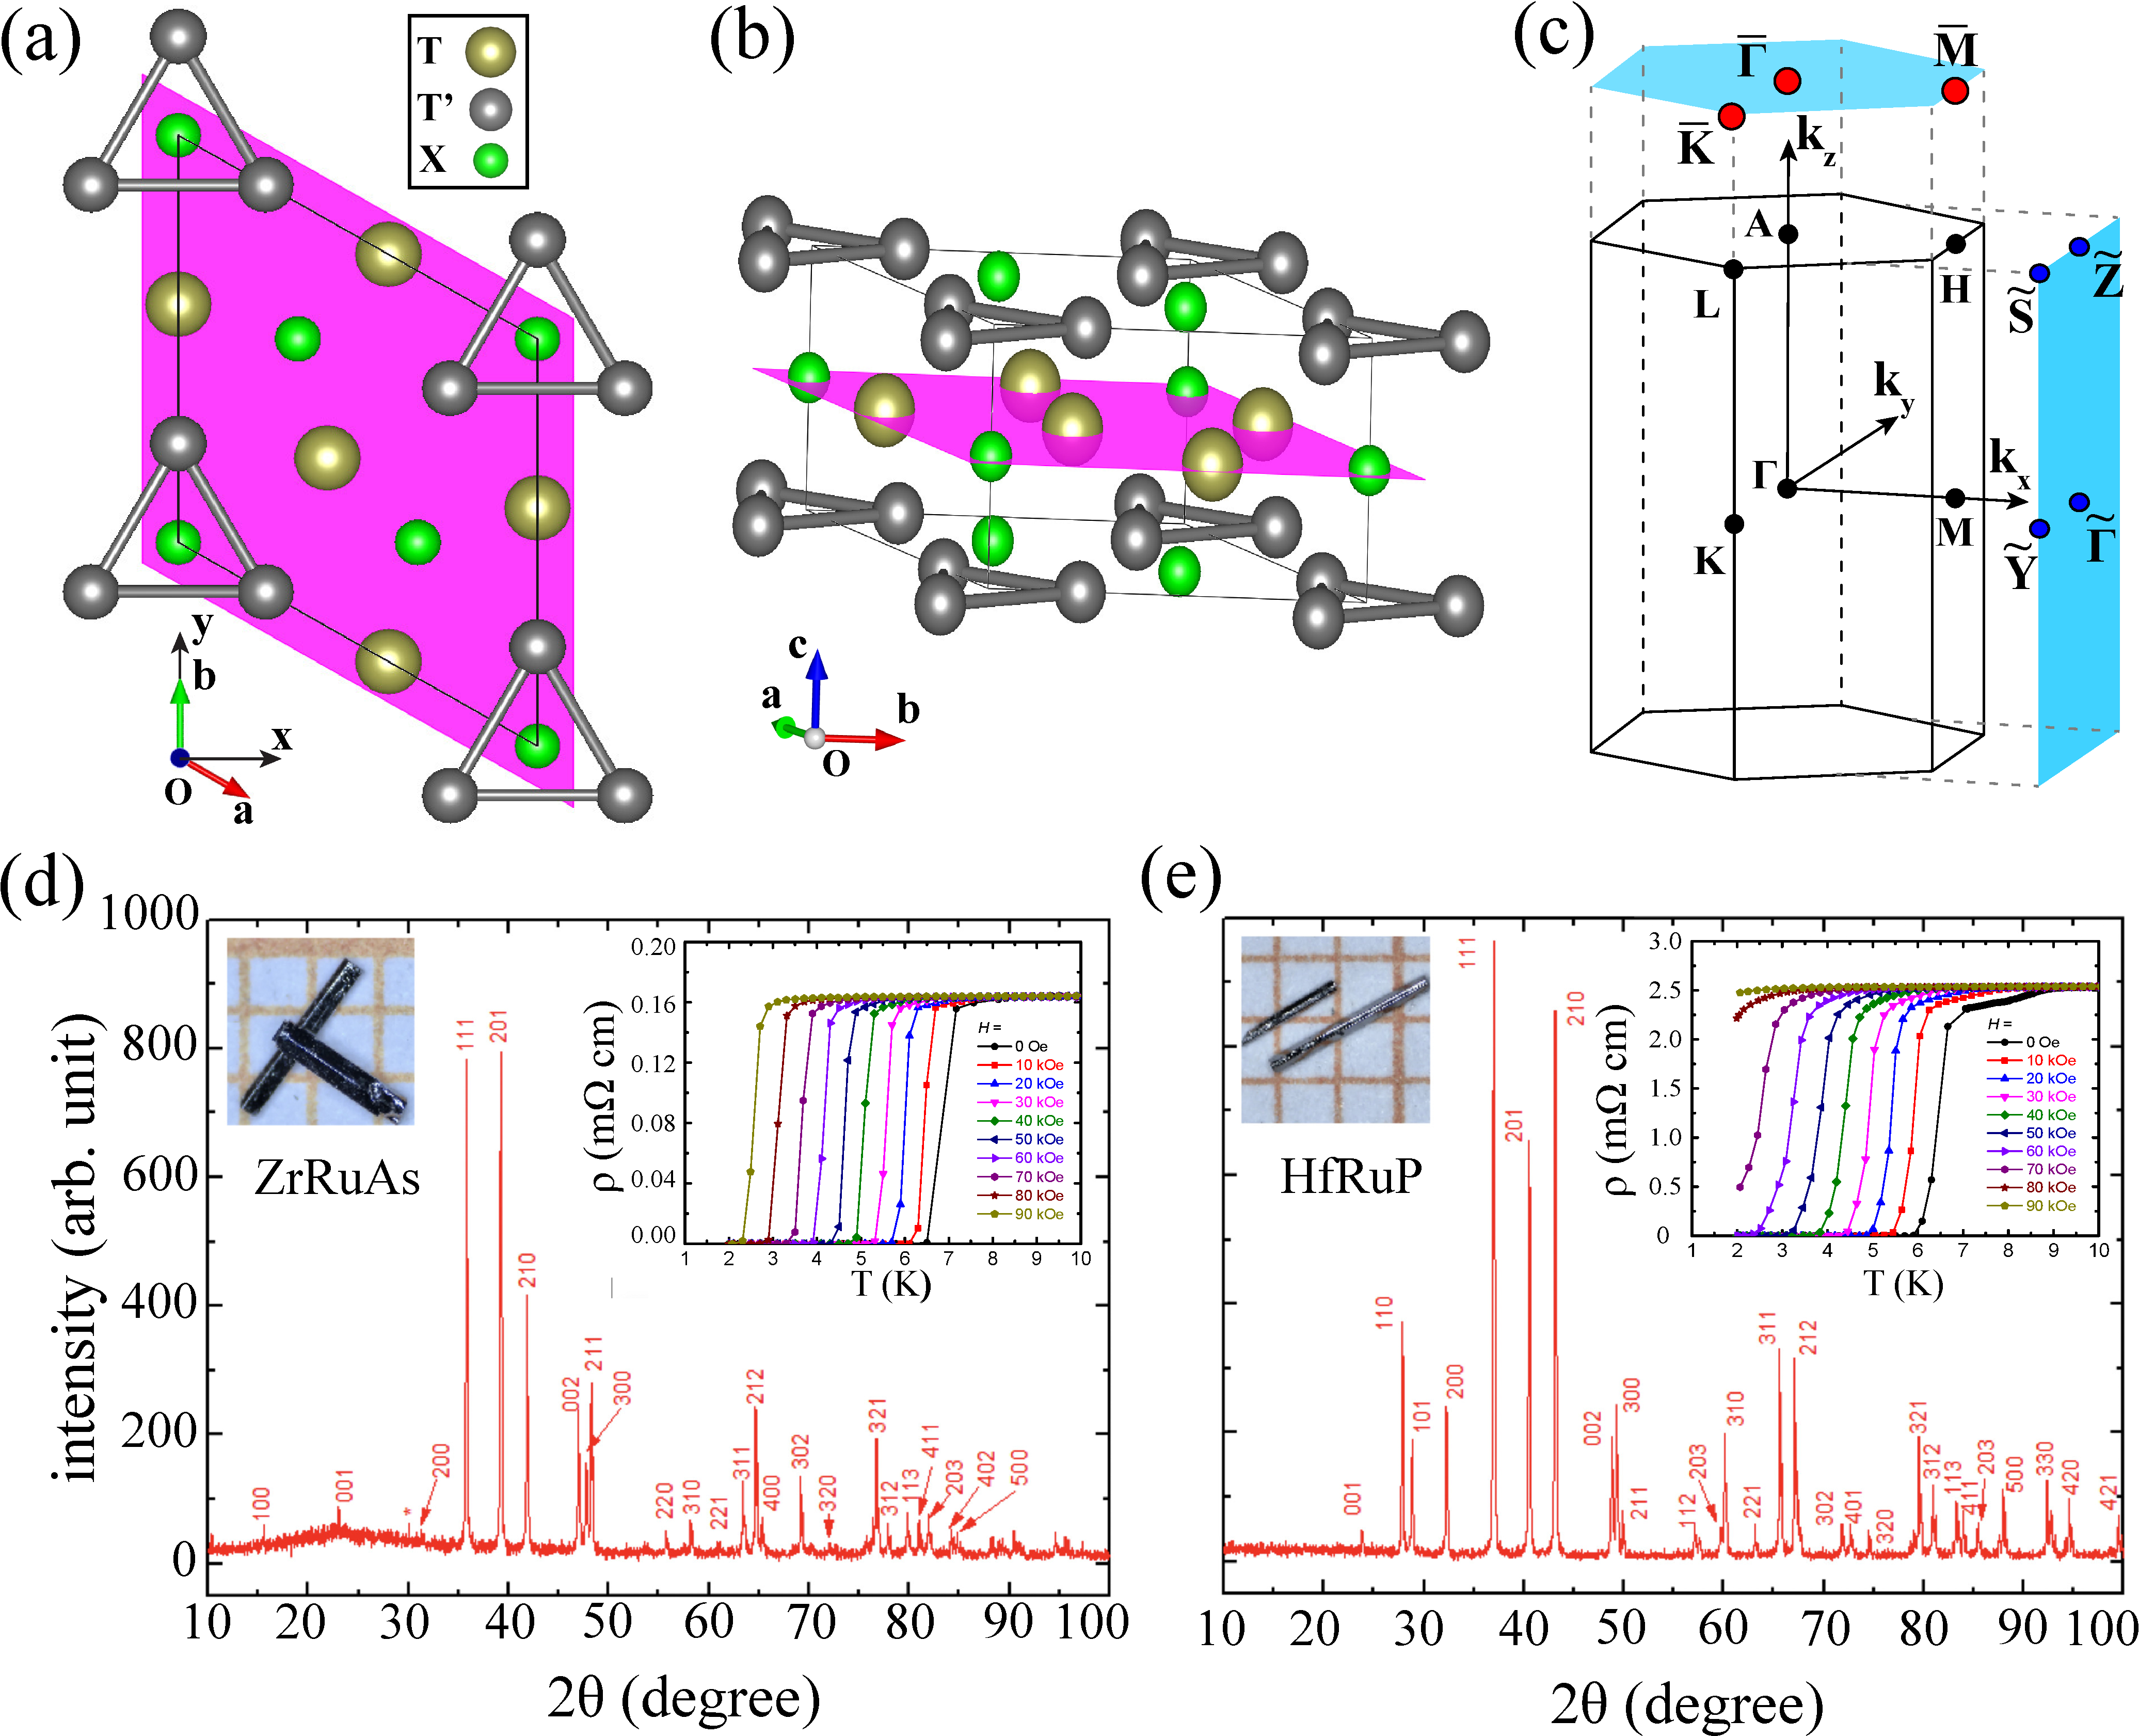
\includegraphics[width=14 cm]{hfrup-fig1.pdf}
    \bicaption{
        TT'X的晶体结构,布里渊区,X射线衍射谱(XRD)和输运性质。(a)晶体结构俯视图:棕色,灰色,绿色分别代表T, T' 和X 原子。
        (b) 晶体的透视图。 
        (c)体布里渊区,(001)-表面布里渊区和(100)-表面布里渊区。此后,(001)[(100) 或(010)] 代表笛卡尔坐标系下表面的法向量。
        (d)和(e)分别为ZrRuAs和HfRuP的索引粉末XRD光谱。红色的星是一小部分杂质。(d)和(e)左边的插图分别是ZrRuAs和HfRuP的单晶样品的照片,右边插图是ZrRuAs和HfRuP在各种磁场下随温度变化的纵向电阻率。 磁场垂直于$ c $轴和电流方向。~\citep{qian2019npj}}
     {The crystal structure, BZs, XRD spectra and transport properties of TT'X.
      ($\bold a$) The top view of the crystal, with brown, gray and green balls representing T, T' and X atoms, respectively.
      ($\bold b$) The perspective view of the crystal. 
      ($\bold c$) The bulk BZ, (001)-surface BZ and (100)-surface BZ. Hereafter, (001) [(100) or (010)] refers to the surface normal vector in terms of the Cartesian coordinates.
      ($\bold d$) and ($\bold e$) Indexed powder XRD spectra of ZrRuAs and HfRuP, respectively. Red stars are small amount of impurities. The left insets of ($\bold d$) and ($\bold e$) are photographs of ZrRuAs and HfRuP single crystals, respectively.  The right insets of them are temperature dependent longitudinal resistivity of ZrRuAs and HfRuP at various magnetic fields. The magnetic fields are perpendicular to $c$ axis and electronic current direction. ~\citep{qian2019npj}
      }
      \label{fig:4-1}
\end{figure}


TT'X的 h- 相空间群是$P\bar 6 2m$ (\#189),层状结构。在六角晶格中每一层被T和X原子或者T'和X原子占据。
所有原子占据在平行于 $ab$- 面的平面内,而且由晶格常数$c$的一半所分开。
三个T'原子(T'$_3$)在 $ab$- 面内形成三角团簇。TT'X的晶体结构如图~\ref{fig:4-1} (a) 和 (b) 所示。T'$_3$团簇和平面结构清晰可见。高对称$\bold{k}$点和表面投影如图~\ref{fig:4-1} (c) 所示。这个结构有两类镜面对称性,$m_z$和$m_x$,这是定义镜面陈数的关键,将在下面讨论。同时,我们也成功生长了单晶样品ZrRuAs和HfRuP,分别展示在图~\ref{fig:4-1} (d) 和 (e) 。 ZrRuP和HfRuP的六角结构通过X射线衍射衍射 (XRD) 得到确认。
ZrRuP和HfRuP的超导性分别由电阻测量(如图~\ref{fig:4-1} (d) 和 (e) 的插入中)和磁化率测量(如图~\ref{hfrup-fig:s6})得到确认。
我们可以看到在温度低于超导相变温度时,两个样品都出现了零电阻现象和迈斯纳效应。


\begin{figure}[!h]
    \centering
    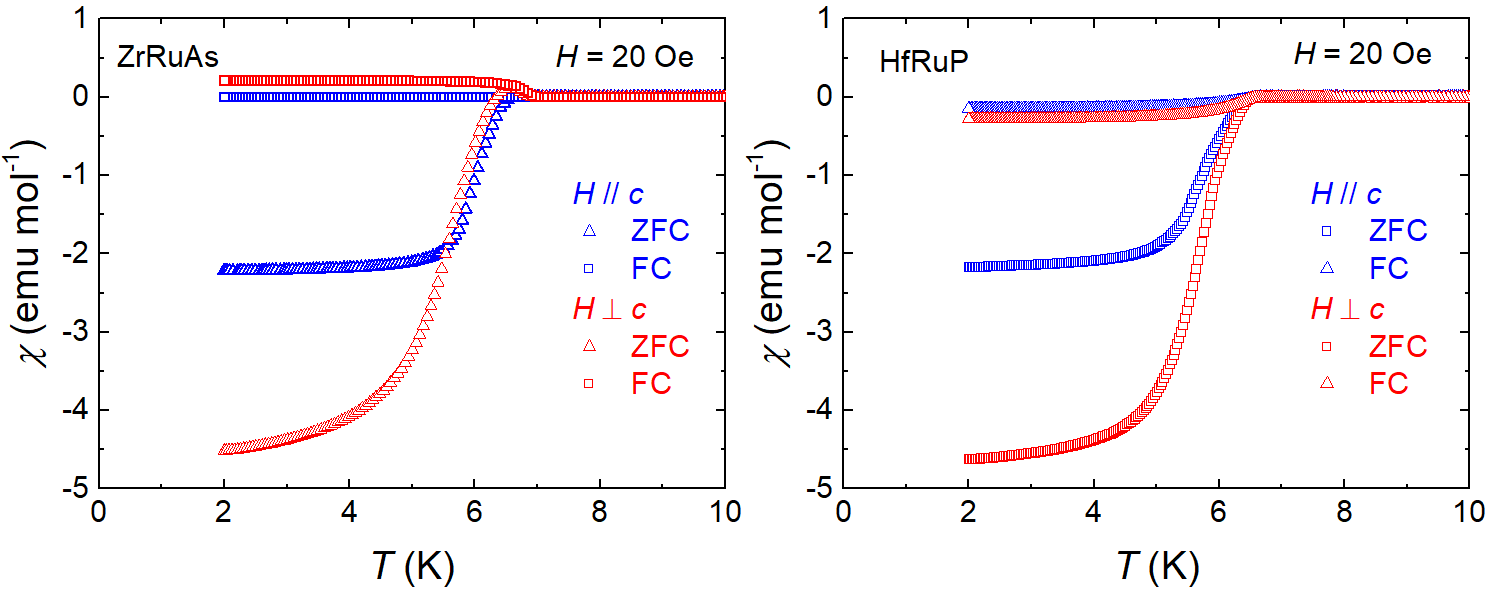
\includegraphics[width=12 cm]{hfrup-figs6.png}
    \bicaption{ (a)ZrRuAs 和(b)HfRuP随温度变化的磁化率曲线。磁场分别垂直于$c$和平行于$c$轴方向施加。~\citep{qian2019npj}}
    {Temperature dependences of magnetic susceptibility of ZrRuAs and HfRuP, respectively. The magnetic field was applied perpendicular and parallel to $c$ axis. ~\citep{qian2019npj}
    }\label{hfrup-fig:s6}
\end{figure}
    

\begin{figure}[!htb]
    \centering
    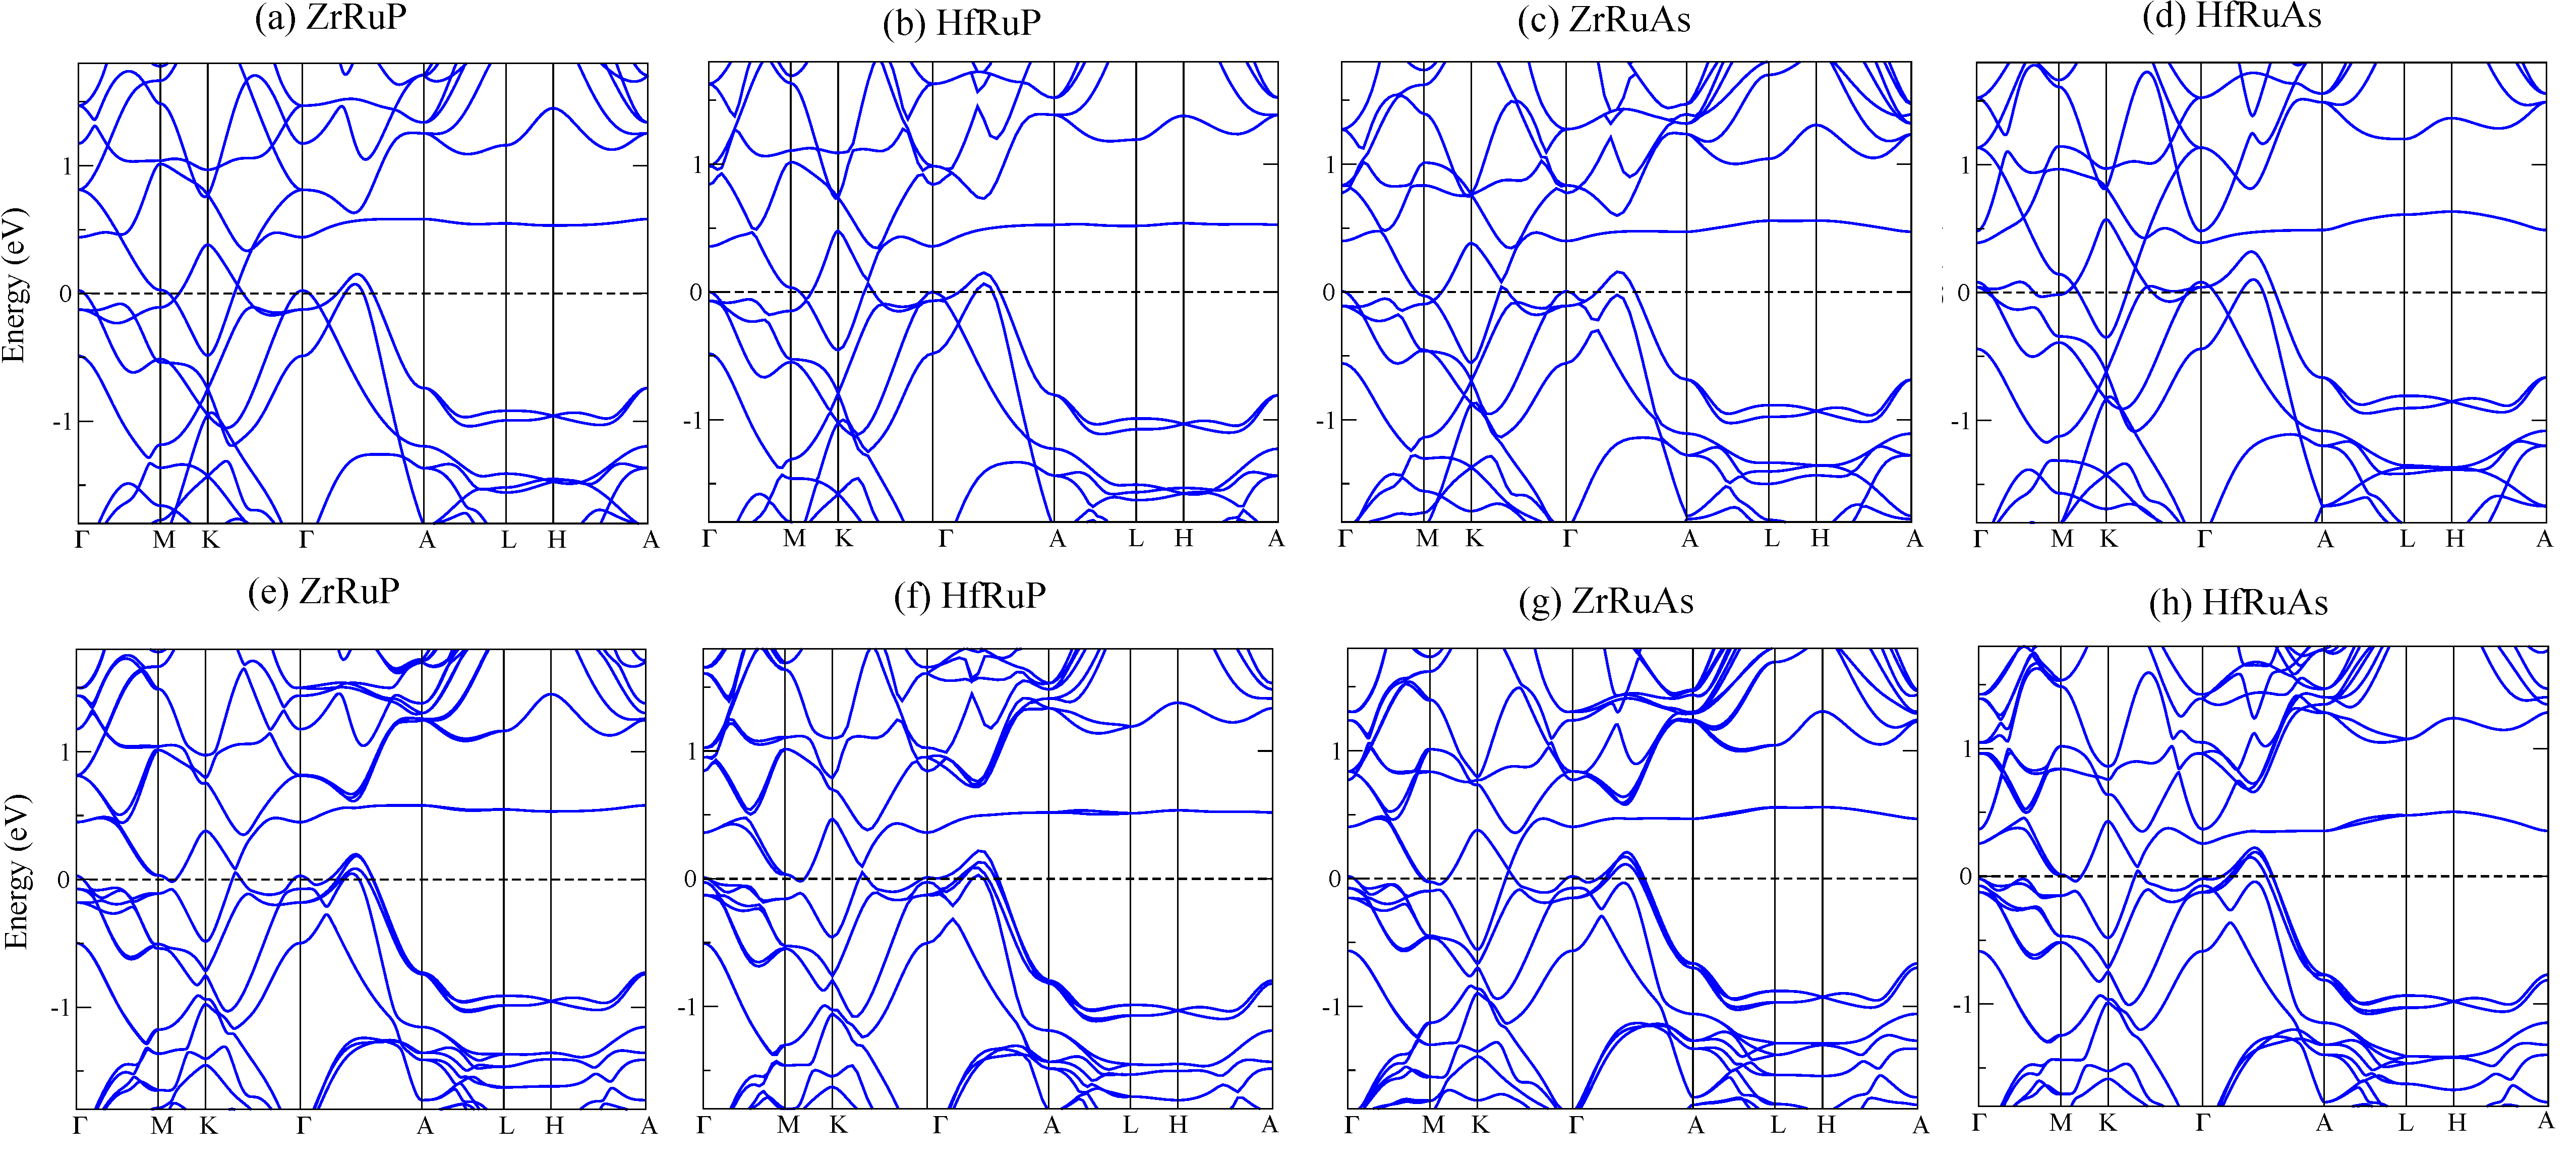
\includegraphics[width=15 cm]{hfrup-figs1.pdf}
    \bicaption{Ru-基化合物(a-d)不考虑SOC和(e-h)考虑SOC的能带结构。~\citep{qian2019npj}}
    {The band structures  of the Ru-based compounds (a-d) without SOC and (e-h) with SOC. ~\citep{qian2019npj}
    }\label{hfrup-fig:s1}
\end{figure}
    
我们首先检查了没有自旋轨道耦合时候的电子结构,如图~\ref{hfrup-fig:s1}。在这些化合物中,我们主要仔细研究了HfRuP和ZrRuAs,分别作为第II类外尔半金属和拓扑晶体绝缘体相的范例。观察~\ref{fig:4-2} (a) 中HfRuP的能带结构,我们发现在靠近费米能E$_F$除了沿着$M-K$和$K-\Gamma$有能带交叉外,其余$\bold{k}$点有直接的带隙(由浅蓝色标出)。事实上,在这两条线在$k_z = 0$的面内,这个面上有$m_z$对称性。两条交叉能带的$m_z$本征值分别为$\pm 1$。因此这两个交点其实是$m_z$保护的节点环的一部分,节点环围绕$k_z = 0$面内的K点,如图~\ref{fig:4-2} (c) 所示。
这与CaAgAs的情况不同 \citep{yamakage2015line},在那里只有一个$\Gamma$点的节点环。
两个绕着两个K点的节点环也在其他化合物中被发现 (参考ZrRuAs,HfRuAs和ZrRuP的能带结构,如图~\ref{hfrup-fig:s1}) 。
我们可以得出结论,能带反转发生在K点,这可以由拓扑量子化学理论支持~\citep{tqc2017,Vergniory2019}。通过交换在K点 (有小群$D_{3h}$) 上最高价带 ($\Gamma_4$) 和最低导带的表示 ($\Gamma_1$) ,占据态能带变成是平庸的,可分解为基本能带表示(EBR)的线性组合~\citep{tqc2017}。

\begin{figure}[!htbp]
\centering
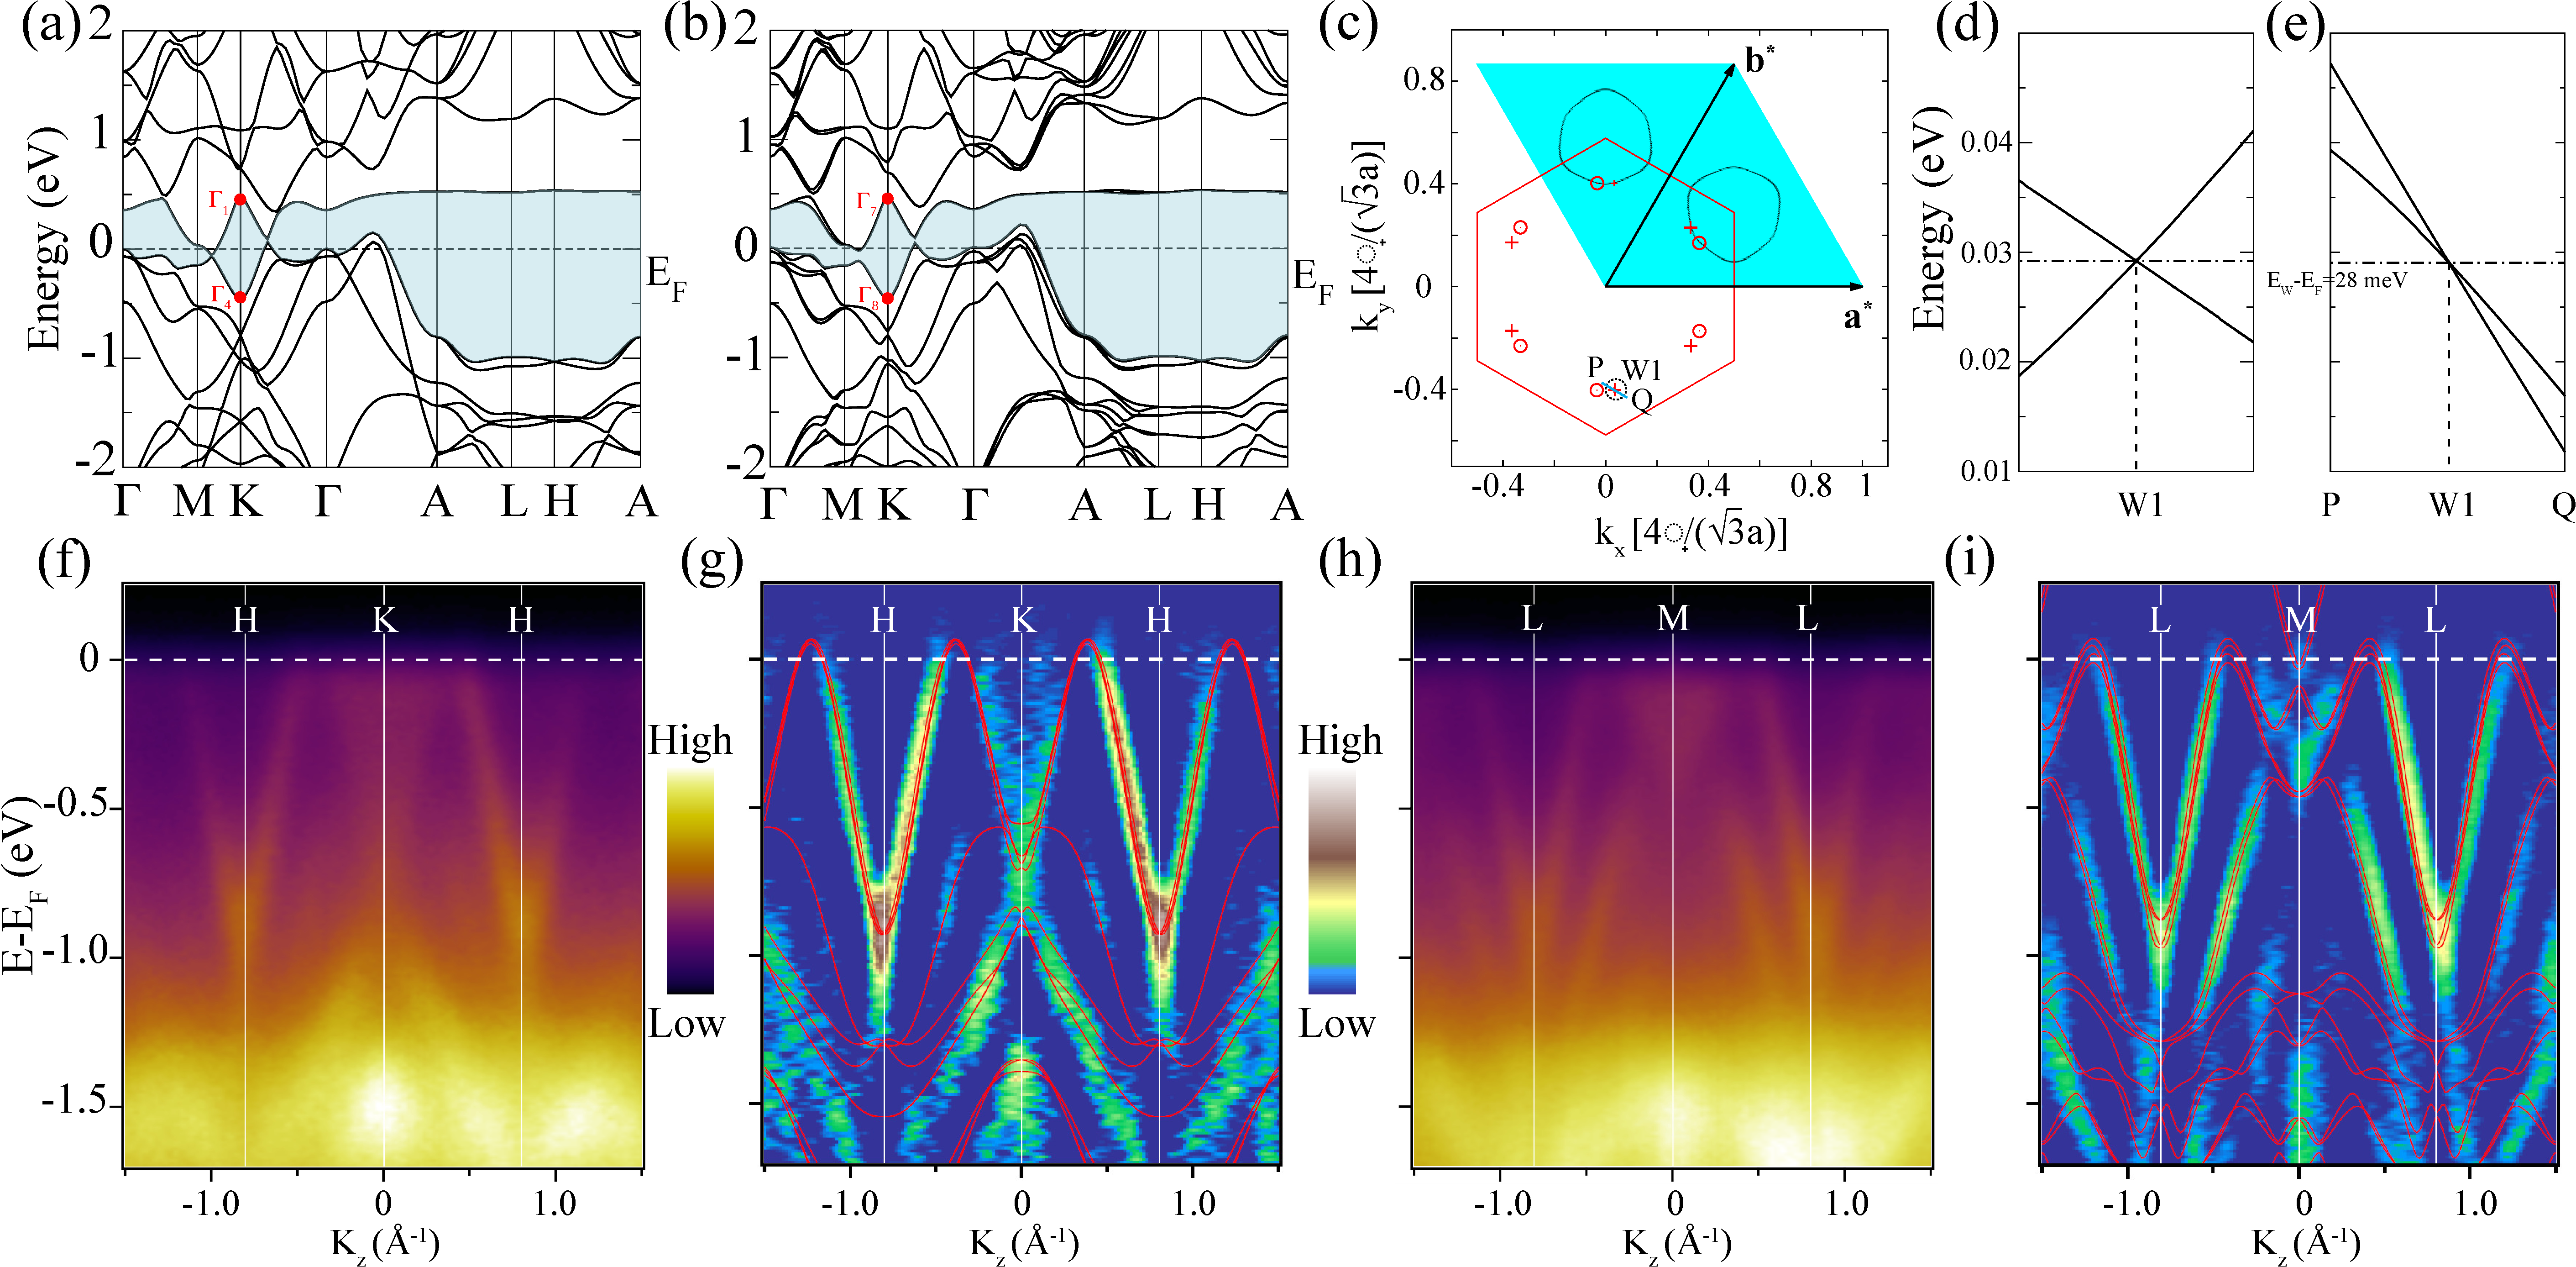
\includegraphics[width=\textwidth]{hfrup-fig2.pdf}
\bicaption{
        在不考虑(a)和考虑(b)SOC时HfRuP的电子能带结构。其中K点选定的能带的不可约表示也标记在图中。
        (c)展示没有SOC时,$k_z=0$面内的节点线。有SOC时,在第一布里渊区里位于$k_z=0$面上方的外尔点标记为 ``+"(+1)和``o"(-1)。
        这里,$\bf a$*,$\bf b$*,和$\bf c$* 是倒空间原胞基矢。
         (d) 穿过外尔点(c)中W1的电子沿着$k_z$方向的能带色散。
         (e)穿过外尔点(c)中W1的电子沿着P-Q方向的能带色散。W1,P和Q的分数坐标分别是$(0.2761 , -0.4654, 0.02439)$和$(0.2603 , -0.4603, 0.02439)$,和$(0.2919 , -0.4705, 0.02439)$。此后,给出的$k$点的位置以($\bf a$*, $\bf b$*, $\bf c$*)为单位。
        ZrRuAs的角分辨光电子谱(ARPES)(f)和曲率强度(g) 展示了沿着H-K-H的能带结构。为了进行比较,图(g) 将沿H-K-H计算的能带结构叠加在实验数据上。(h-i)和(f-g)一样,但是是沿着L-M-L方向的。~\citep{qian2019npj}
        }
        {
        The electronic band structures of HfRuP without (a) and with (b) SOC.
        The irreducible representations of selected bands at K point are indicated.
        (c) The nodal lines are presented in the $k_z=0$ plane without SOC.
        With SOC, the WPs above the $k_z=0$ plane are labeled as ``+"(+1) and ``o"(-1) in the first BZ.
        Here, $\bf a$*, $\bf b$*, and $\bf c$* are the reciprocal primitive vectors.
        (d) The $k_z$ dispersion of the electronic bands through the WP W1 shown in (c).
        (e) The dispersion of the WP W1 along the line P-Q shown in (c).
        The fractional coordinates of W1, P and Q are $(0.2761 , -0.4654, 0.02439)$, $(0.2603 , -0.4603, 0.02439)$, and $(0.2919 , -0.4705, 0.02439)$. Hereafter, the positions of $k$-points are given in units of ($\bf a$*, $\bf b$*, $\bf c$*).
        ARPES spectrum (f) and curvature intensity (g) plots of ZrRuAs, showing band structure along H-K-H. For comparison, the calculated band structure along H-K-H is superposed on the experimental data in (g). (h-i) are the same as (f-g), but along L-M-L. ~\citep{qian2019npj}}
\label{fig:4-2}
\end{figure}
    
在考虑自旋轨道耦合之后,能带结构变化不大,但是由于缺少中心反演对称性,能带发生劈裂。
为了确认密度泛函理论 (DFT) 得到的能带结构的可靠性,我们对ZrRuAs进行了ARPES测量,展示在图~\ref{fig:4-2} (f) - (i) 。沿着H-K-H和L-M-L观察到的谱与DFT计算结果 (图~\ref{fig:4-2} (g) 和 (i) 中红色的线) 吻合的非常好,特别是对于低能的能带。我们可以很清楚的看到,K点的能带比M点能带更低。另外,两条简并的节点环由于SOC而打开。二维时间反演不变的平面 (如 $k_y = 0$和$k_z = 0$等面) 完全打开能隙,使得$\mathbb Z_2$不变量可以很好的定义。在CaAgAs中,绕着$\Gamma$点的单个的节点环由于有限的SOC强度使得$k_y = 0$ (或者$k_z = 0$)面是$\mathbb Z_2$不平庸的。但是这和两个K点有两个节点环的ZrRuAs情况不同。对于这些化合物,$k_y = 0$和$k_z = 0$两个面的 $\mathbb Z_2$不变量仍然是平庸的。注意$k_y = 0$即使是没有SOC也是打开能隙的,而且在所有时间反演不变的平面都没有能隙闭合的点。为了确定$\mathbb Z_2$不变量是平庸的,在 $k_y = 0$ ($k_z = 0$) 面,我们计算了$k_z$- 指向的 ($k_y$- 指向的) Wilson loop的瓦尼尔心作为$k_x$的函数 (称为Wilson-loop bands) 。ZrRuAs的结果如图~\ref{hfrup-fig:s2} (a) 和 (b) ,在$k_y = 0$ 面和$k_z = 0$面$\mathbb Z_2$不变量是平庸的。其余的四个时间反演不变的平面的$\mathbb Z_2$不变量细节也展示在图~\ref{hfrup-fig:s2}。类似地,所有这些化合物的Fu-Kane $\mathbb Z_2$指标~\citep{Fu2007topo} 为 (0;000) 。

\begin{figure}[!htb]
    \centering
    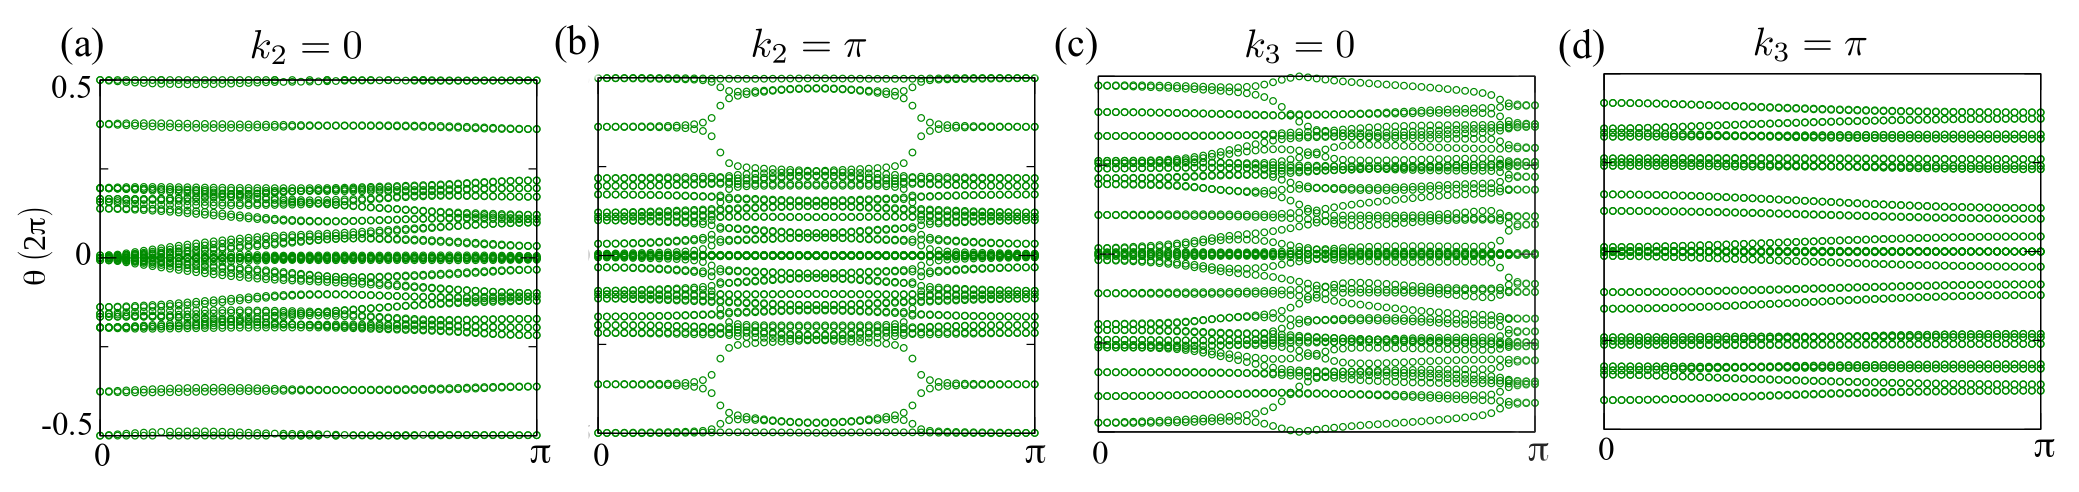
\includegraphics[width=1\textwidth]{hfrup-figs2z2}
    \bicaption{ZrRuAs四个时间反演不变平面内占据态能带的Wannier心的演化。~\citep{qian2019npj}}{
    The flow of WCCs for all occupied energy bands in four TRI planes of ZrRuAs. ~\citep{qian2019npj}
    }\label{hfrup-fig:s2}
\end{figure}
    
我们进一步发现这些材料的对称性指标~\citep{nc_ashvin,song2017,Jorrit2017,zhang2019,wanxg2019} 为$\mathbb Z_{3m,0}=1$和$\mathbb Z_{3m,\pi}=0$,揭示了SOC能隙如图~\ref{fig:4-2} (b) 的拓扑本质。
    
      
\subsection{镜面陈数和外尔点}
\begin{figure}[!htbp]
    \centering
    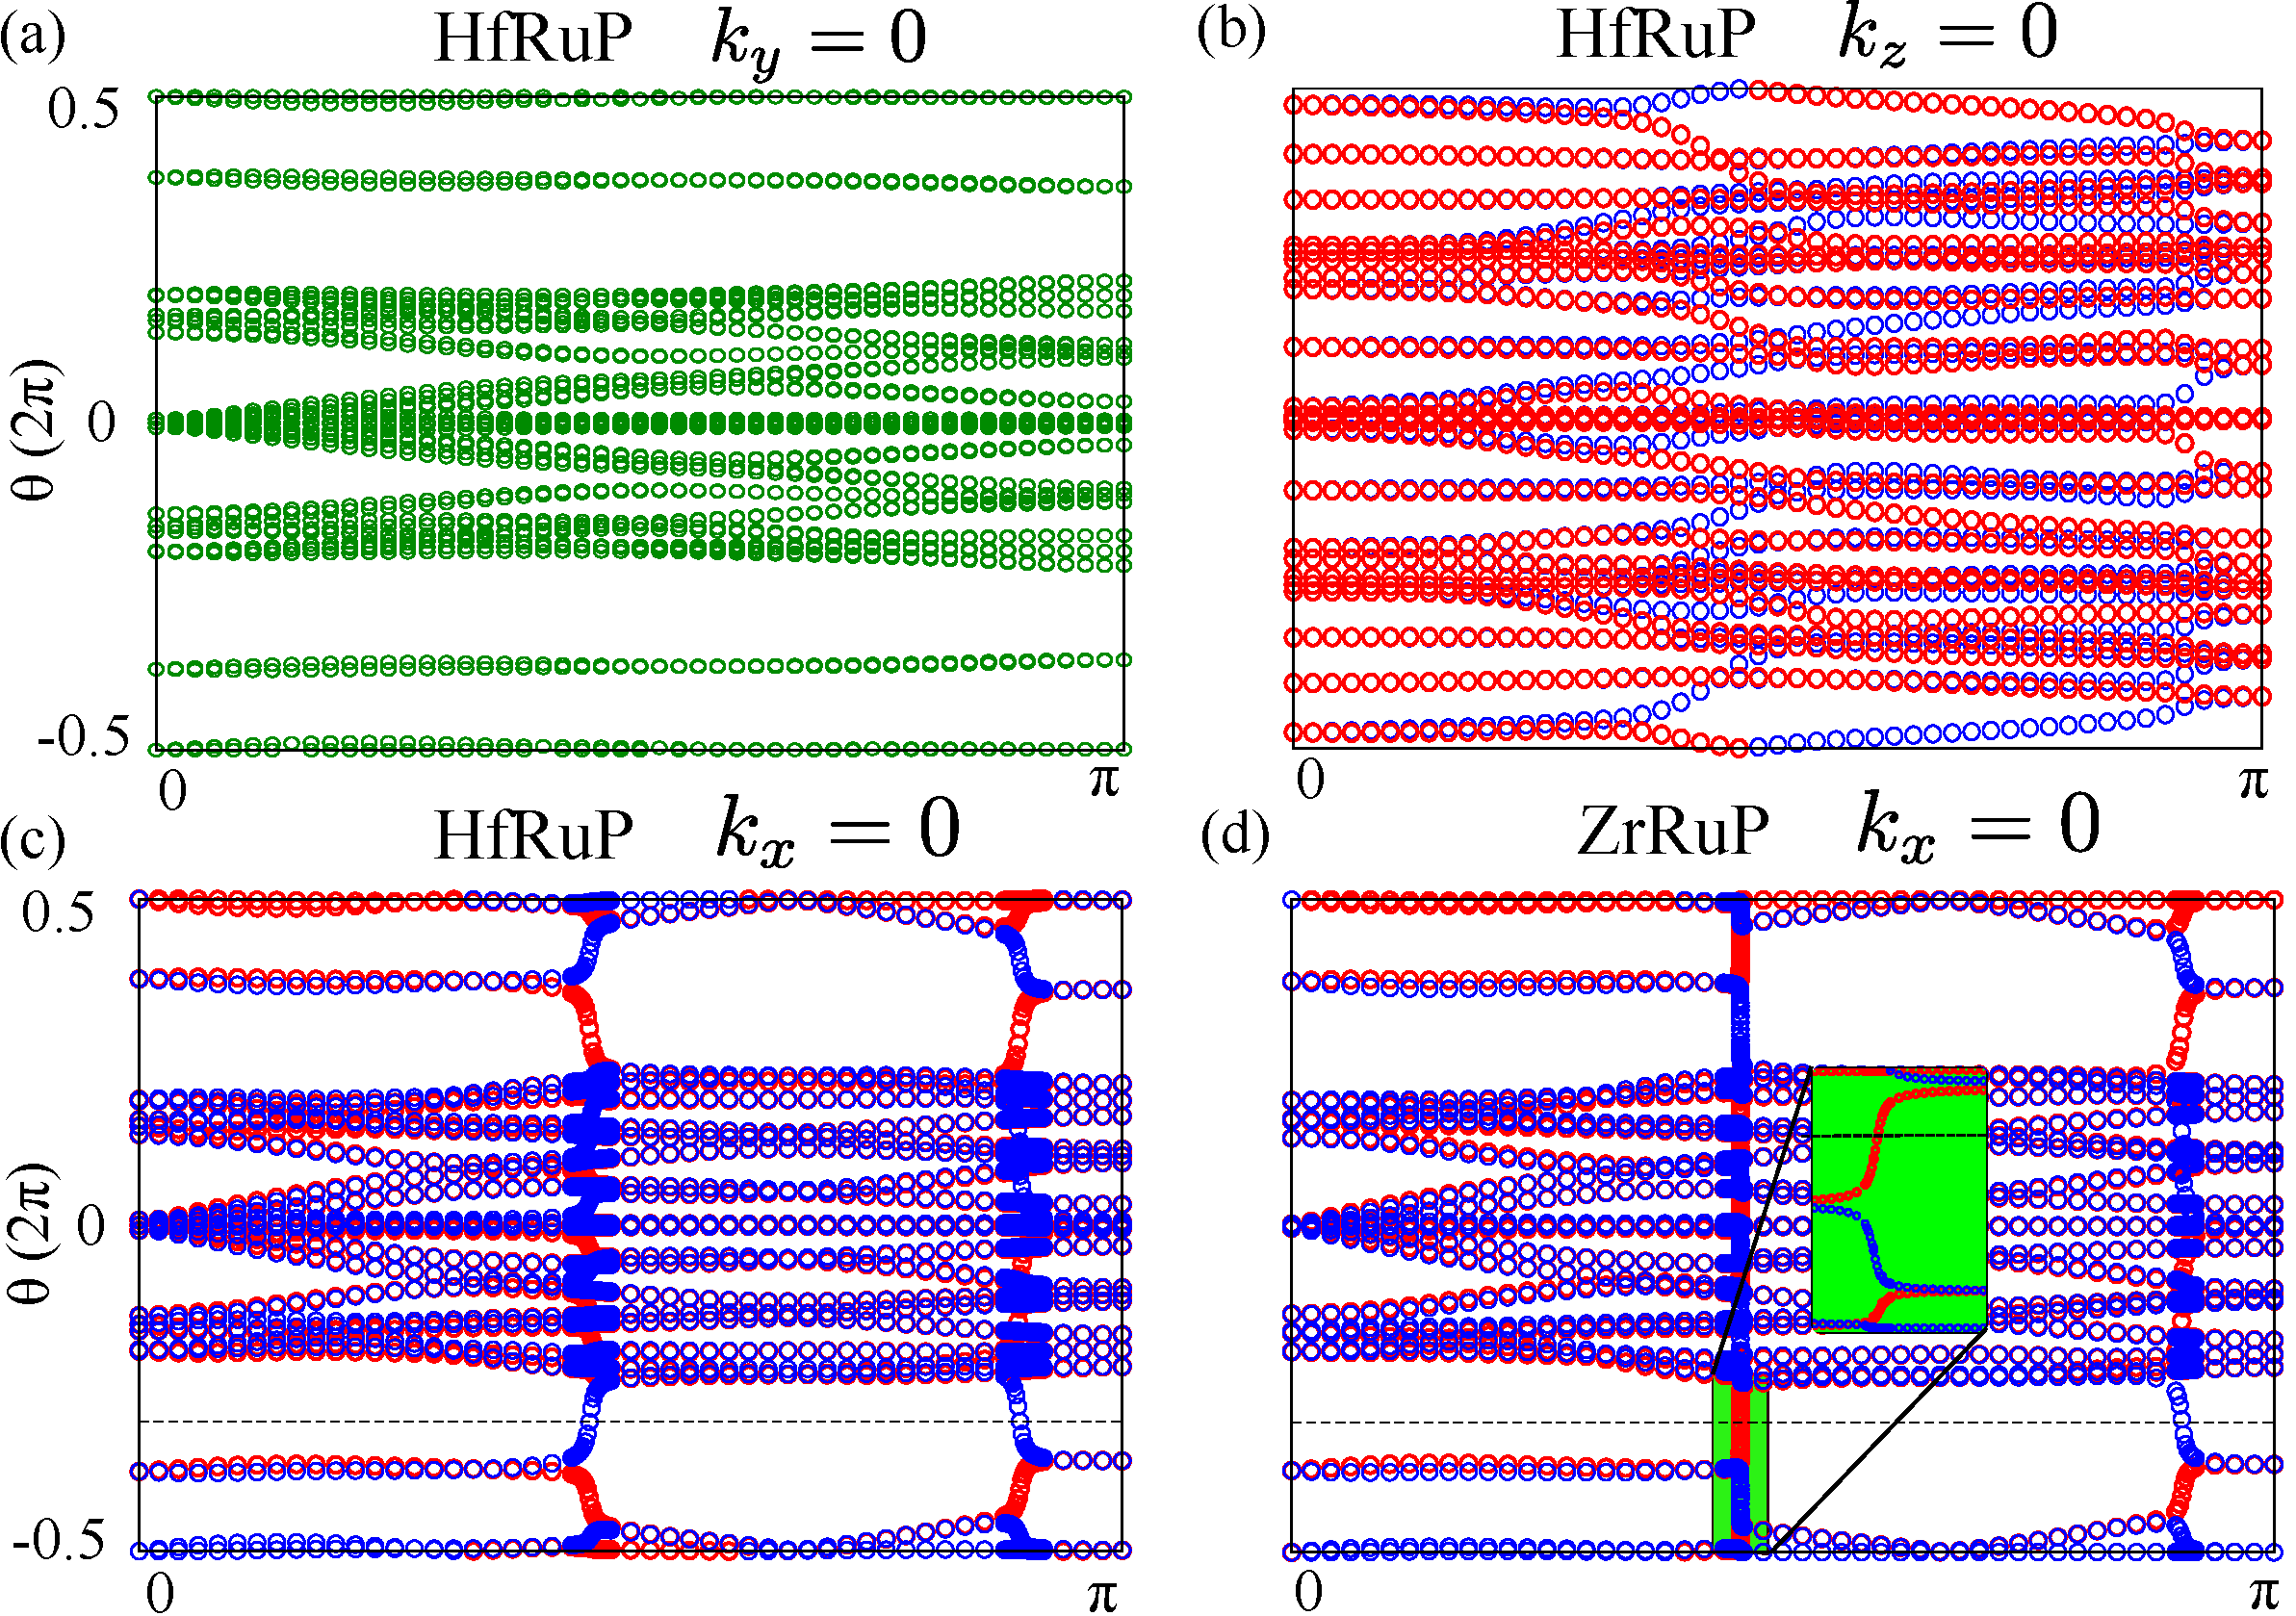
\includegraphics[width=0.8\textwidth]{hfrup-fig3.pdf}
    \bicaption
    {时间反演不变平面上的瓦尼尔电荷中心(WCC)。
    (a)和(b)分别为$k_y = 0$ 和$k_z = 0$面作为$k_x$函数的$k_z$- 指向和 $k_y$- 指向的Wilson loops。
    (c)和(d)分别为HfRuP 和 ZrRuAs在$k_x = 0$面内作为$k_y$函数的$k_z$ - 指向的Wilson loops。
    红色和蓝色的圈分别代表有镜面本征值为$+i$和$-i$的能带的WCC流。水平的虚线代表参考线。~\citep{qian2019npj}
    }
    {The WCCs of TRI planes.
    (a) and (b) The WCCs of the $k_z$-directed and $k_y$-directed Wilson loops as a function of $k_x$ for the $k_y = 0$ and $k_z = 0$ planes, respectively.
    (c) and (d) The WCCs of the $k_z$-directed Wilson loops as a function of $k_y$ in the $k_x = 0$ plane of HfRuP and ZrRuAs, respectively.
    Red and blue circles represent the flow of the WCCs for the bands with mirror $+i$ and $-i$ eigenvalues, respectively.
    The horizontal dashed lines are reference lines. ~\citep{qian2019npj}}
    \label{fig:4-3}
\end{figure}    
    
    
由于镜面对称性的出现,只要镜面上的能带完全打开能隙,镜面陈数就可以很好的定义。因为时间反演对称操作和镜面对称操作对易,陈数满足$C_i =  -C_{-i}$,下标$\pm i$代表有SOC时的镜面本征值。镜面陈数可以定义为$C_m = (C_{+i}-C_{-i})/2$。众所周知,在半个镜面上,这可以进一步推导为$\chi_{+i}-\chi_{-i}$,其中$\chi_{+i(-i)}$可以很容易的通过画Wilson-loop bands,通过在 $+i~(-i)$子空间数水平参考线[如图~\ref{fig:4-3} (c) 和 (d) 中的虚线]与斜率为正的能带相交的次数减去与斜率为负的能带相交的次数。对于$k_x = 0$平面,ZrRuAs的计算结果如图~\ref{fig:4-3} (d) 。ZrRuAs的$k_z$ = 0的镜面陈数$C_{m_z}$ 计算结果为$-2$,而$k_z =\pi$的镜面陈数为0。这个家族的所有化合物的镜面陈数情况如图~\ref{hfrup-fig:s3}。

\begin{figure}[!htb]
    \centering
    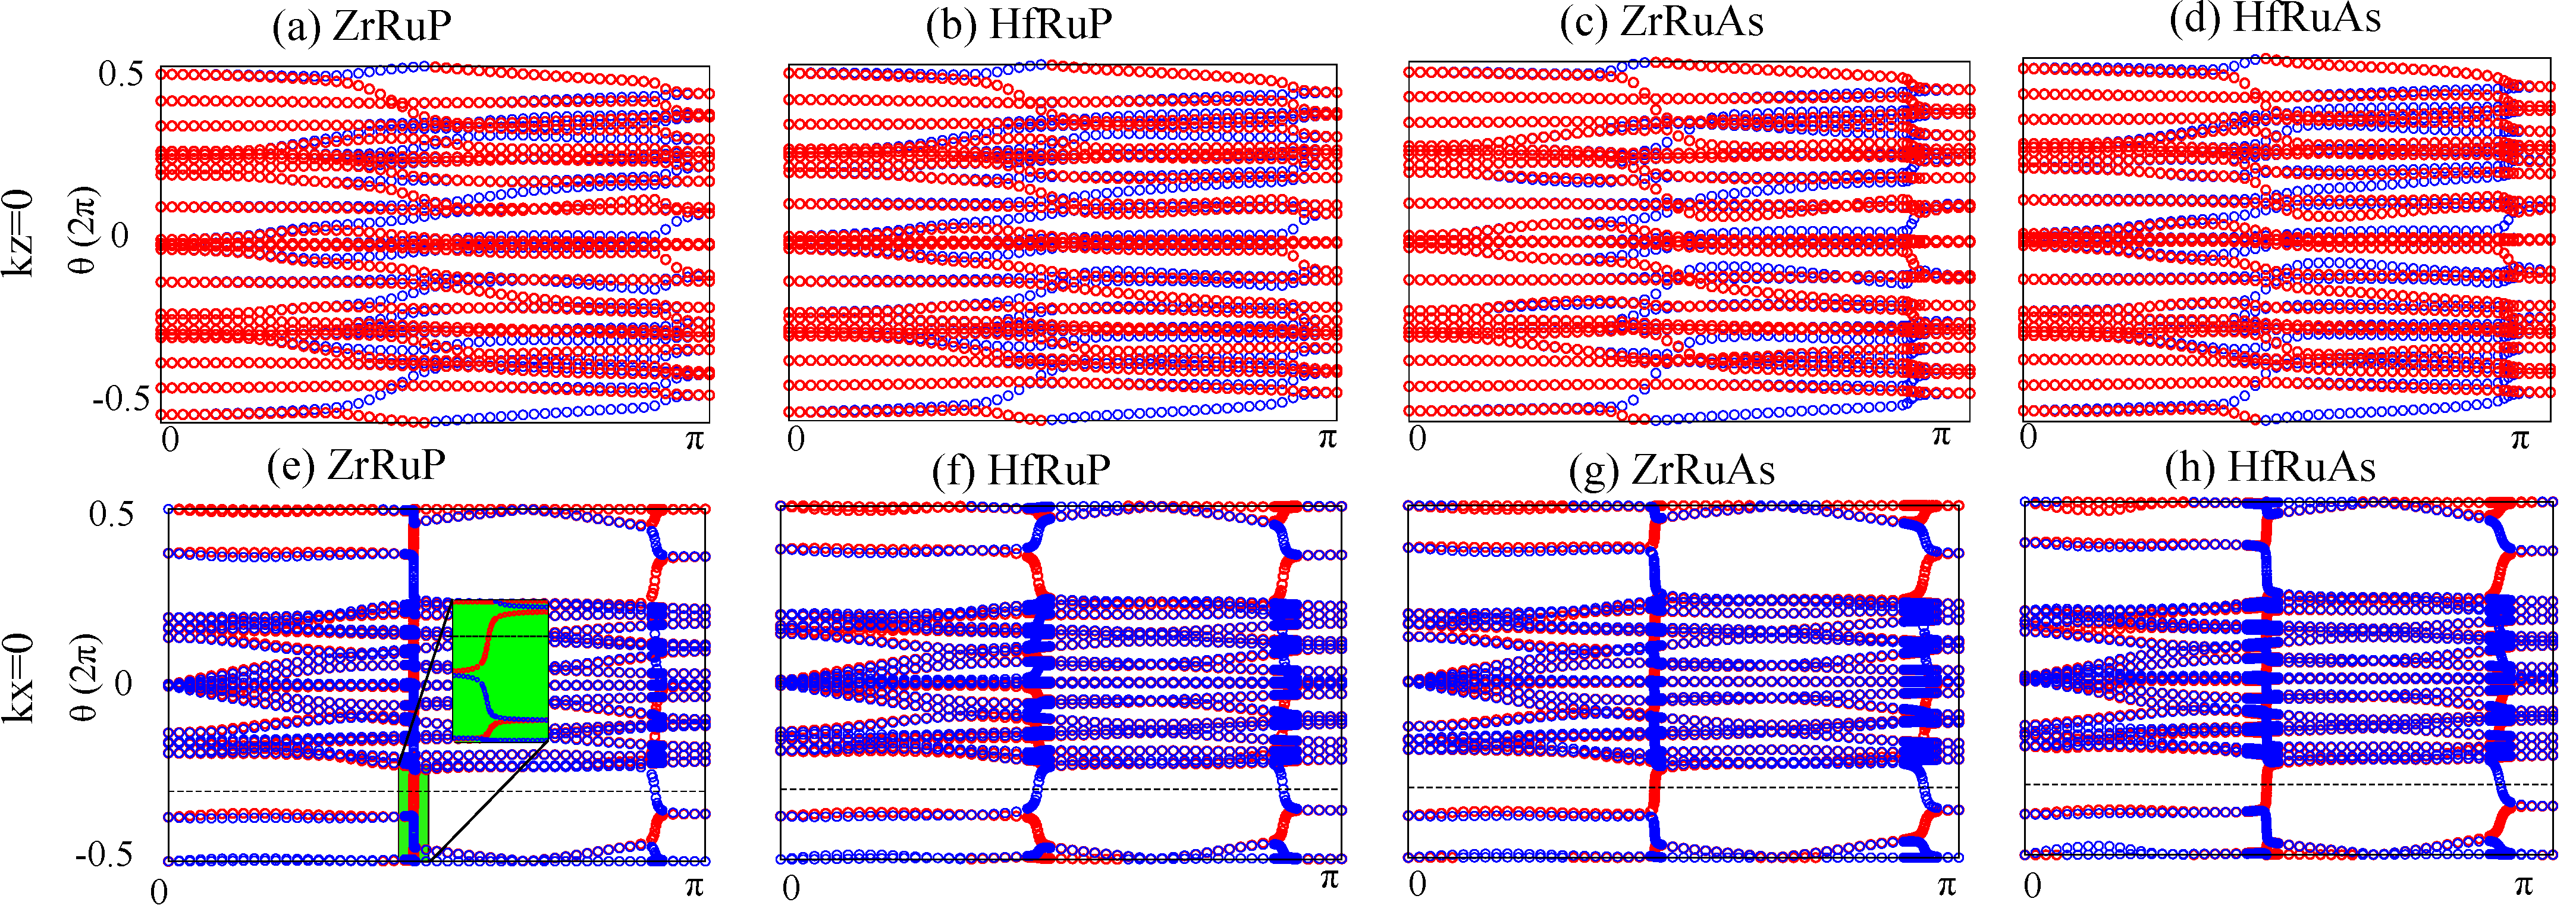
\includegraphics[width=1\textwidth]{hfrup-figs3}
    \bicaption{ 当考虑自旋轨道耦合时,Ru-基化合物在(a-d)$k_x=0$ 和(e-h)$k_z=0$ 面的镜面陈数。红色的圈代表镜面本征值为$+i$的能带的WCCs流,蓝色的圈代表镜面本征值为$-i$的能带的WCCs流。
    在(e-h)中,黑色虚线是任意选择的参考线,目的是为了看参考线和Wilson-loop正负斜率的能带交叉的次数。(e)中放大的插图显示了连接方式的细节。~\citep{qian2019npj}}
    {
    The mirror Chern numbers of Ru-based compounds  for (a-d) $k_x=0$ and (e-h) $k_z=0$ planes when SOC is considered. Red circles represent the flow of the WCCs for bands with mirror $+i$  eigenvalue and blue circles for bands with mirror $-i$  eigenvalue.
    The black dashed line in (e-h) is an arbitrarily selected reference line for the purpose of counting the number of crossing times between the reference line and the Wilson-loop bands with positive and negative slopes. The zoom-in inset of (e) shows the connective pattern clearly. ~\citep{qian2019npj}
    }\label{hfrup-fig:s3}
\end{figure}
    
    
中心对称性的破缺允许系统中出现外尔点。非零的镜面陈数$C_{m_z} =-2$ 表明在$ k_z = 0 $平面中存在一些规范奇异的线穿过\citep{bernevig2015s},这必须在三维布里渊区的某些外尔点上终止。我们系统的计算表明,根据$k_x=0$面上的镜面陈数$C_{m_x}$不同,这些化合物可以分为两类:i)一类有为零的镜面陈数 $C_{m_x} =0$,这类有12对第II类外尔点,称为外尔半金属相; ii) 另一类有非零的镜面陈数 $C_{m_x} =2$,这一类没有外尔点,称之为拓扑晶体绝缘体相。HfRuP在 $k_x=0$面的瓦尼尔电荷中心如图~\ref{fig:4-3} (c) ,镜面陈数 $C_{m_x}$为0。不能完全补偿的$m_z$和$m_x$ 面的镜面陈数表明系统中存在外尔点,而且在这个材料中确实发现了外尔点,这和外尔半金属相相吻合。但是,对于ZrRuAs,HfRuAs和ZrRuP,$C_{m_x}$计算表明是$2$,如图\ref{fig:4-3} (d) 和图~\ref{hfrup-fig:s3}。由于镜面陈数完全补偿,所以这些系统中不存在外尔点。事实上,在这几个材料中我们也确实没有发现外尔点存在。

通过检查能隙和相关的拓扑单极电荷,我们发现从每个节点环产生6对外尔点。因此在第一布里渊区共有12对外尔点如图~\ref{fig:4-2} (c) 。他们处于同样的能量,因为他们由时间反演对称性和晶体对称性$D_{3h}$ (包括12个对称操作)相联系。在图~\ref{fig:4-2} (c) 中,由虚线包围的外尔点W1的坐标是[0.2761$\bf a$*, $-$0.4654$\bf b$*, 0.02439$\bf c$*]。 从W1沿着$k_z$- 方向 [图~\ref{fig:4-2}(d)]和P-Q 方向[图~\ref{fig:4-2}(e)]的色散,我们可以知道它属于第II类外尔点~\citep{xu2015},它的能量(E$_W$)在费米能E$_F$以上28 meV (即E$_W$-E$_F= 28$ meV),非常接近费米能。拓扑单极电荷可以由包裹外尔点的闭合流型上计算Wilson-loop的方法获得。外尔点W1的单极电荷是+1。$k_z = 0$面以上所有外尔点的分布如图~\ref{fig:4-2} (c) ,``+(o)" 代表拓扑电荷$+1(-1)$,而在$k_z = 0$以下的外尔点由于$m_z$对称性有相反的单极电荷,如图~\ref{fig:4-2} (c) 。
    
    
\subsection{表面态上的费米弧}
\begin{figure}[!htbp]
    \centering
    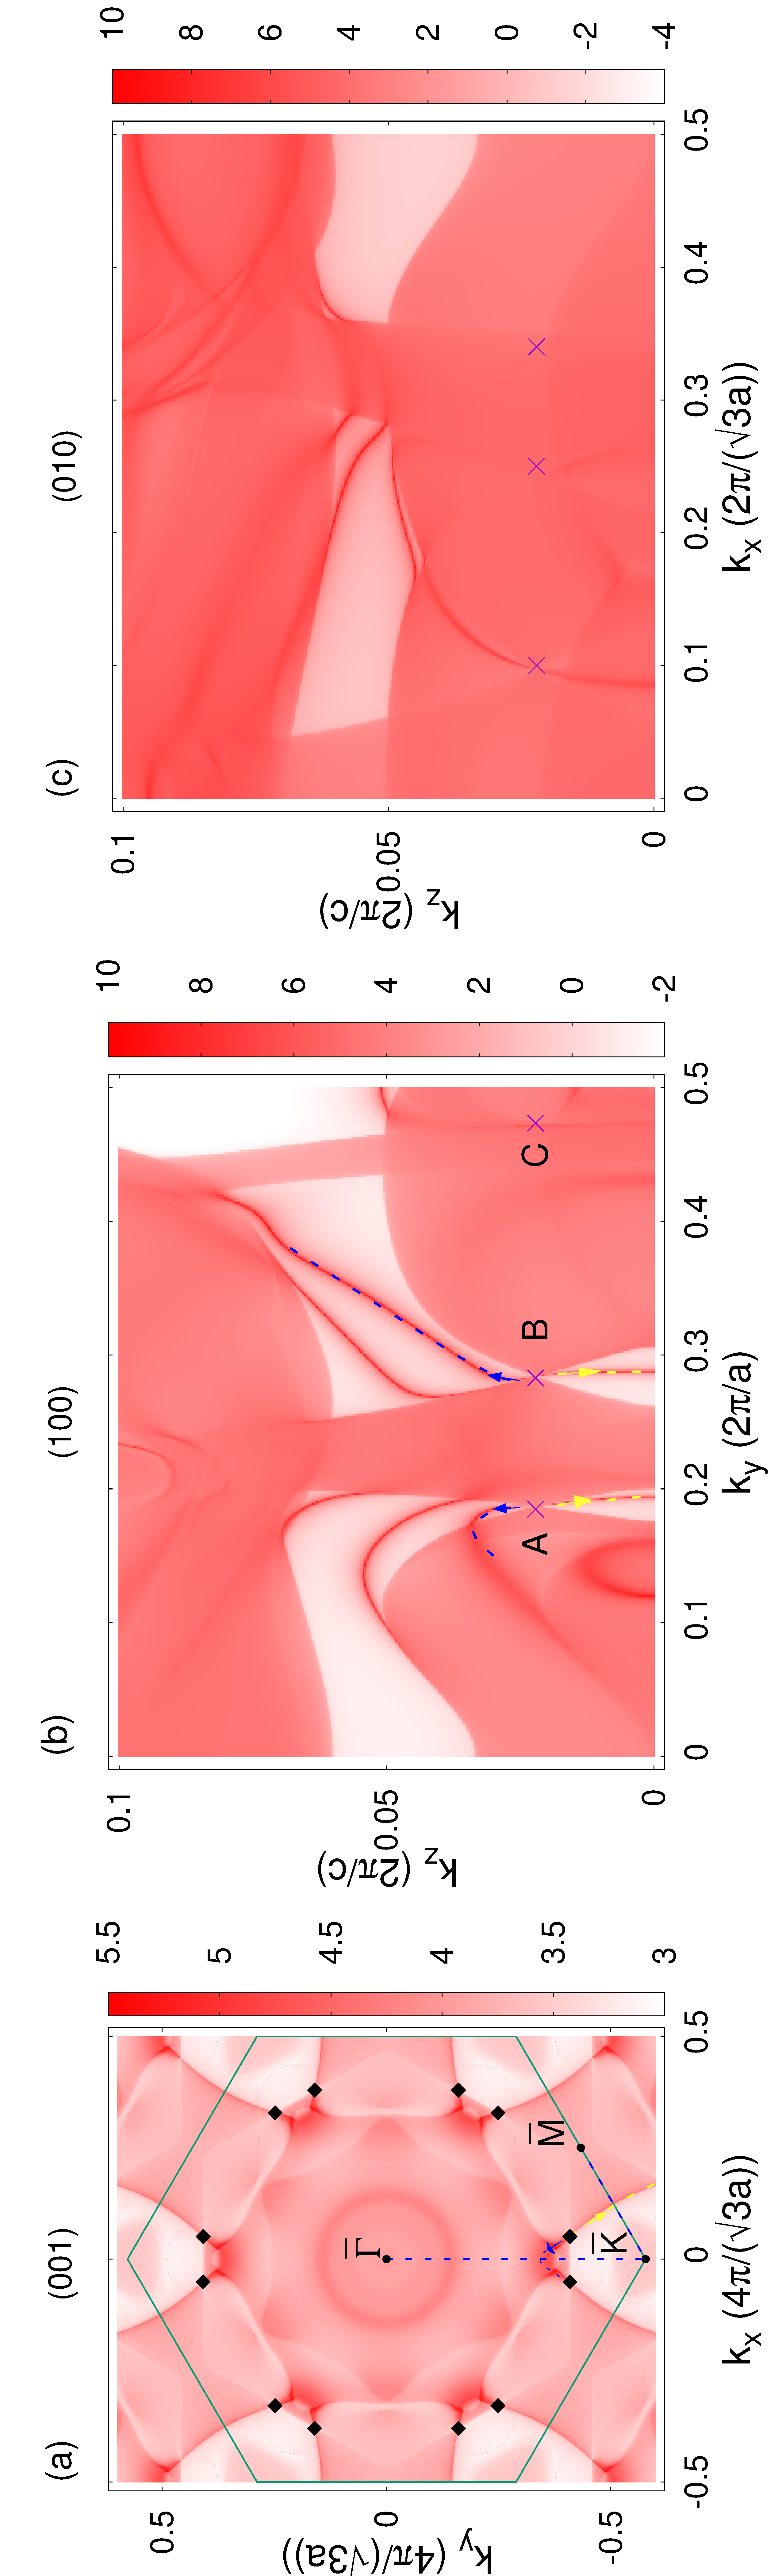
\includegraphics[angle=270,width=14 cm]{hfrup-fig4.pdf}
    \bicaption{
    HfRuP的表面谱。(001)- 表面(a),(100)- 表面(b)和(010)- 表面(c) 能量为$E-E_W=0$ meV的表面谱。
    外尔点的投影用菱形或``x''符号标记。~\citep{qian2019npj}}
    {
    The surface spectra of HfRuP. The (001)-surface (a), (100)-surface (c) and (010)-surface (c) energy contours with $E-E_W=0$ meV.
    The projections of the WPs are indicated by diamonds or ``x" symbols. ~\citep{qian2019npj}
    }
    \label{fig:4-4}
\end{figure}    

\begin{figure}[!h]
    \centering
    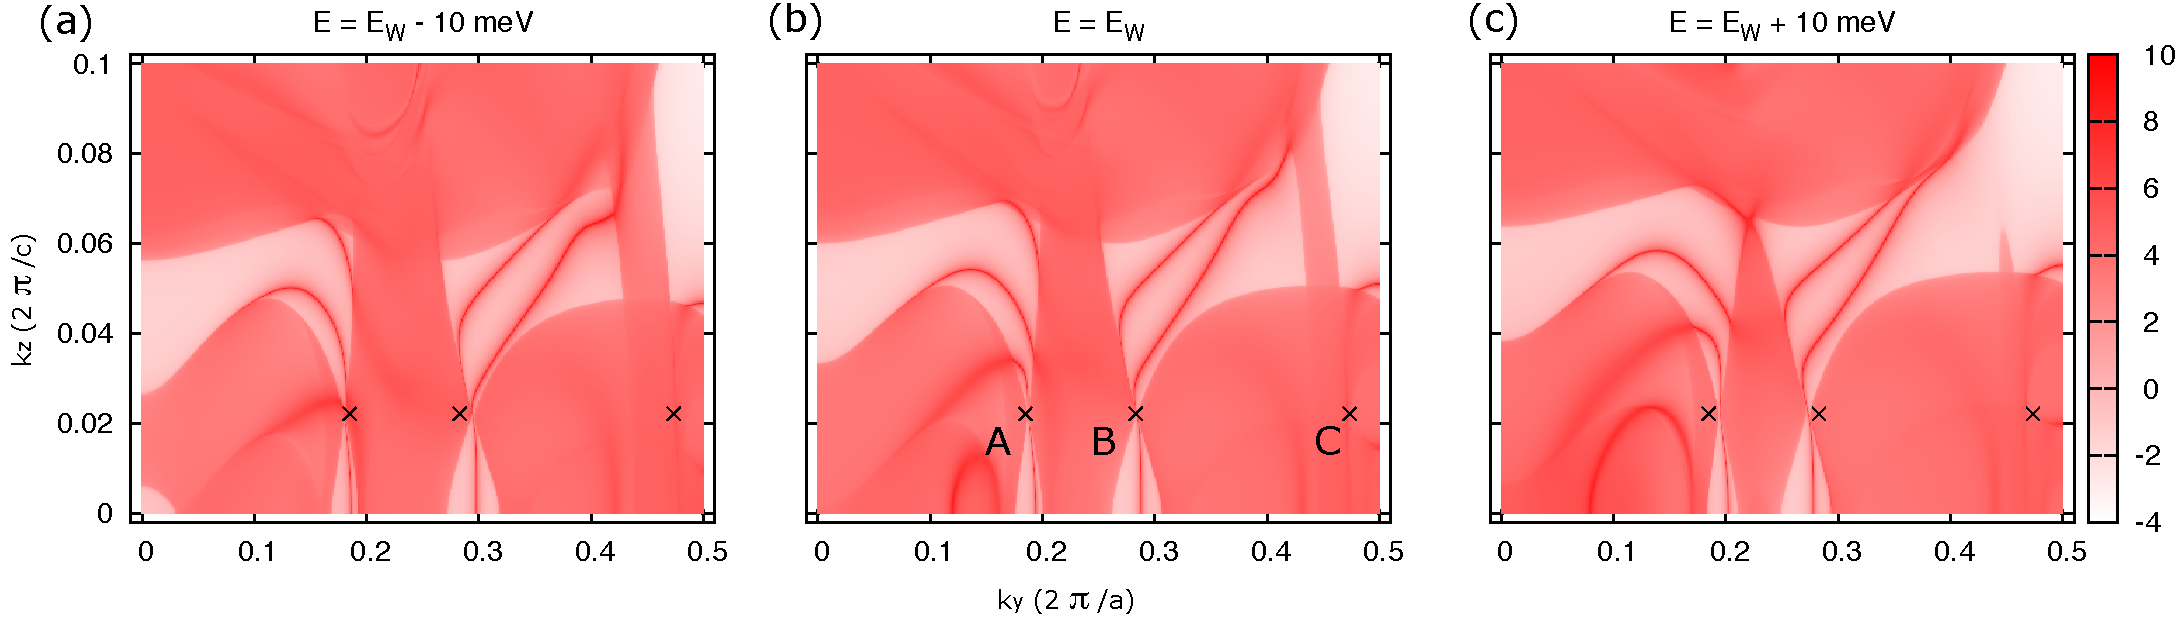
\includegraphics[width=14 cm]{hfrup-figs4}
    %\includegraphics[width=16 cm]{figs3}
    \bicaption{不同等能面外尔点的投影。E$_W$是外尔点所处的能量位置。~\citep{qian2019npj}}
    {
    The different energy contours with the projections of WPs.
    E$_W$ is the energy level of the WPs. ~\citep{qian2019npj}
    }\label{hfrup-fig:s4}
\end{figure}
  
在外尔半金属中,我们期望出现连接两个手性相反的外尔点的投影的表面费米弧。为了这个目的,基于格林函数的方法\citep{Sancho_1985},我们计算了半无限大的最局域化的瓦尼尔函数的表面态。首先,在图~\ref{fig:4-4} (a) 中给出了HfRuP的(001)表面能量为$E-E_W=0$ meV的表面态。因为在 (001) 表面两个手性相反的外尔点投影到同一个点,所以不能保证从投影的点出发有拓扑的费米弧表面态。但是,我们发现有两条平庸的arc态从每个外尔点的投影出来:一个arc穿过$k_x = 0$的线;另一个穿过布里渊区边界,(即, $\bar K- \bar M$线)。其次,计算的(100)等能面如图~\ref{fig:4-4} (b) 所示。因为他们是第II类外尔点,外尔点应该位于电子口袋和空穴口袋相接触的点。我们也确实看到了在两个口袋接触点的地方有外尔点的投影A和B。我们看到了两条表面费米弧(用虚线标记)连接投影点 (即,A和B) 。对于投影点C,很难看到任何从它出发的表面态,因为它没有投影到一个合适的表面上。最后,计算的 (010) 表面的等能面如图~\ref{fig:4-4} (c) ,其中相同手性的外尔点投影到一起。只要电子/空穴口袋 (包裹外尔点的投影) 彼此分开,我们就可以期望出现两条拓扑的费米弧态。但是不幸的是,金属型的体态在很大的范围内都有投影,这使得费米弧态无法看到。我们在(100)表面寻找费米弧的ARPES实验仍在进行中。
  
这些外尔点是第二类外尔点,为了解释这一点,我们画了(001)表面在能量稍微低于或者高于E$_{W}$的常数能量的等能面的表面态展示在图~\ref{hfrup-fig:s4}。
从低一点的能量 (E=E$_W$-10 meV) 到更高一点能量 (E=E$_W$+10 meV) , 我们可以清楚的看到外尔点的投影 (例如 A点 或者 B点) 从一个口袋变到另一个口袋。从投影C点, 很难看到类似点演化过程,因为没有投影到合适的方向。
%%%%  

\subsection{新奇的拓扑超导态}
凭借固有的超导性,由于在正常状态下波函数具有非平凡的拓扑结构,拓扑材料是实现拓扑超导的有前途的平台。例如,表面狄拉克费米子甚至可以在$ s $波配对状态下实现二维拓扑超导\citep{Fu2008superconducting,wang2015}。而且,正常态费米面的拓扑会直接影响拓扑超导性。在三维,在时间反演不变的超导体中整数的拓扑量子数由配对序参量的符号和在费米面上的贝利相位规范场的第一陈数决定~\citep{qi2011}。超导体中的外尔半金属相有来源于外尔点的不平庸的拓扑。HfRuP的外尔半金属相提供了两个关键要素:非平庸的费米面和超导电性,可以作为实现3D时间反演不变的拓扑超导的良好平台。除此之外,之前的工作~\citep{shingo2015,ueno2013}报道了不平庸的镜面陈数可以产生Cd$_3$As$_2$和SrRuO$_4$中的多重Majorana费米子。这些化合物中的拓扑晶体绝缘体相也是寻找拓扑晶体超导体的极有希望的候选者。
    
\section{结论}
基于DFT计算,我们发现TT'X的 h- 相在没有SOC的能带结构有两个节点环,这与CaAgAs不同。在考虑SOC后,这些化合物或者进入有12对第II类外尔点的外尔半金属相,或者进入有非零陈数的拓扑晶体绝缘体相。两个不同相的单晶样品已经成功生长出来。他们的超导性和电子能带结构通过我们电阻测量,磁化率,和ARPES测量的分别得到验证。这一系列Ru基化合物都是单晶化合物,在T$_C$以下有超导性,在T$_C$ 以上有拓扑性。这项工作将促进对超导性与外尔或非平庸镜面陈数态之间相互作用的实验研究。
 

\chapter{拓扑晶体绝缘体LaSbTe的层构造}\label{chap:lasbte}



\section{背景}
拓扑晶体绝缘体~\citep{fu2011topological}是由时间反演对称性保护的拓扑绝缘体~\citep{TIreview,qi2011,weng2015quantum}之外的一种由晶体对称性保护的拓扑态。由晶体平移对称性保护的三维弱拓扑绝缘体可以通过在第三个方向堆叠二维拓扑绝缘体得到。受此启发,除了平移对称性之外,由镜面对称性保护的拓扑晶体绝缘体也已经被发现可以绝热地连接到弱耦合的二维拓扑态极限,而这些二维的拓扑态可以是由镜面对称性保护的拓扑晶体绝缘体~\citep{kim2015},也可以是二维拓扑绝缘体~\citep{Fulga2016}。这些发现启发研究者们基于“降维理论”研究拓扑晶体绝缘体,现在称之为“层构造(LC)”方法。已经证明,所有的由晶体点群对称性保护的拓扑态都可以通过堆叠更低维度的拓扑态来获得,而且因此得到的拓扑分类既可以应用于相互作用的玻色子,也可以应用于自由费米子~\citep{huang2017,hsong2017,Songreal,Song2019}。通过这种方法,可以清晰地理解晶体对称性保护的拓扑态的物理本质。

我们所的方辰老师团队非常详细地利用了层构造方法,他们在存在时间反演对称性的情况下,推导出了从对称数据到任意空间群的拓扑不变量之间详尽的映射关系~\citep{song2017}。当与拓扑量子化学和对称性指标~\citep{tqc2017,nc_ashvin,Kruthoff2017}相结合时,这种映射关系提供了非常有效的方法来定义和搜索新的拓扑晶体绝缘体。层构造方法是用具有不平庸的$\mathbb{Z_2}$或者镜面陈数的二维绝缘体来搭建晶格,而原子绝缘体是由放在Wyckoff位置上合适的原子轨道组成。然而,层构造和所形成的拓扑晶体绝缘体之间的对应关系不像原子绝缘体的物理图像那么清晰。最近,Matsugatani和Watanabe使用紧束缚模型将高阶拓扑绝缘体与低维的拓扑态相联系,来展现高阶拓扑绝缘体的物理本质~\citep{haruki2018}。但是,目前还没有一个能够将实空间的低维拓扑态和动量空间能带拓扑之间精确的一对一关系展现出来的、实际的层状拓扑晶体绝缘体材料。

在我们的工作中,我们介绍了一个实际材料LaSbTe,这个材料有两个相:四方相($\tlasbte$)和正交相($\olasbte$),其中$\tlasbte$是$WHM$($W$ = Zr,Hf或La,$H$ =Si,Ge,Sn,或Sb,和$M$ = O,S,Se,或Te)家族的一员~\citep{xu2015two}。当考虑自旋轨道耦合时,$\tlasbte$是每一个原胞内有一个二维拓扑绝缘体的弱拓扑绝缘体,而由两个$\tlasbte$沿着堆叠方向发生了结构相变产生的$\olasbte$是原胞内有两个二维拓扑绝缘体的拓扑晶体绝缘体。因此$\olasbte$可以看作是两个有一定晶格畸变的$\tlasbte$,其中每个$\tlasbte$代表一个“基本层构造”(eLC)的一层。据我们所知,这是第一个能解释LC方法的例子,换句话说,是第一个能够清晰地将实空间层构造与倒空间能带拓扑映射的材料,这为理解拓扑晶体绝缘体的物理图像提供了很好的平台。


\section{晶体结构和计算方法}
{\it{计算方法}}:第一原理计算中采用了基于密度泛函理论的VASP程序包~\citep{KRESSE199615,vasp} 和投影缀加平面波(PAW)的方法~\citep{paw1,paw2} 。Perdew-Burke-Ernzerhof类型的广义梯度近似(GGA)~\citep{pbe}作为交换相关泛函。平面波截断能为300 eV。对于$\tlasbte$和$\olasbte$自洽计算过程中布里渊区$\mathbf{k}$点取样分别为
为$8\times 8 \times 4$和$12\times 12 \times 3$。在高斯展宽方法中,采用0.02eV的宽度确定费米能级。我们采用了实验晶格参数~\citep{charvillat1977cristallochimie,dimasi1996stability} ,然后完全弛豫结构,直到所有原子上的力均小于0.01 eV/\AA。
考虑和不考虑SOC的能带结构都做了相应都计算。基于Wannier90~\citep{mlwf}构造的最局域Wannier函数,采用WannierTools软件包\cite{WU2017}来计算表面态。采用基于密度泛函微扰理论(DFPT)~\citep{togo2015first}的Phonopy程序来计算声子谱。使用了Wilson-loop技术来计算单层的时间反演$\mathbb{Z}_2$。

%%figure
\begin{figure}[!t]
    \centering
    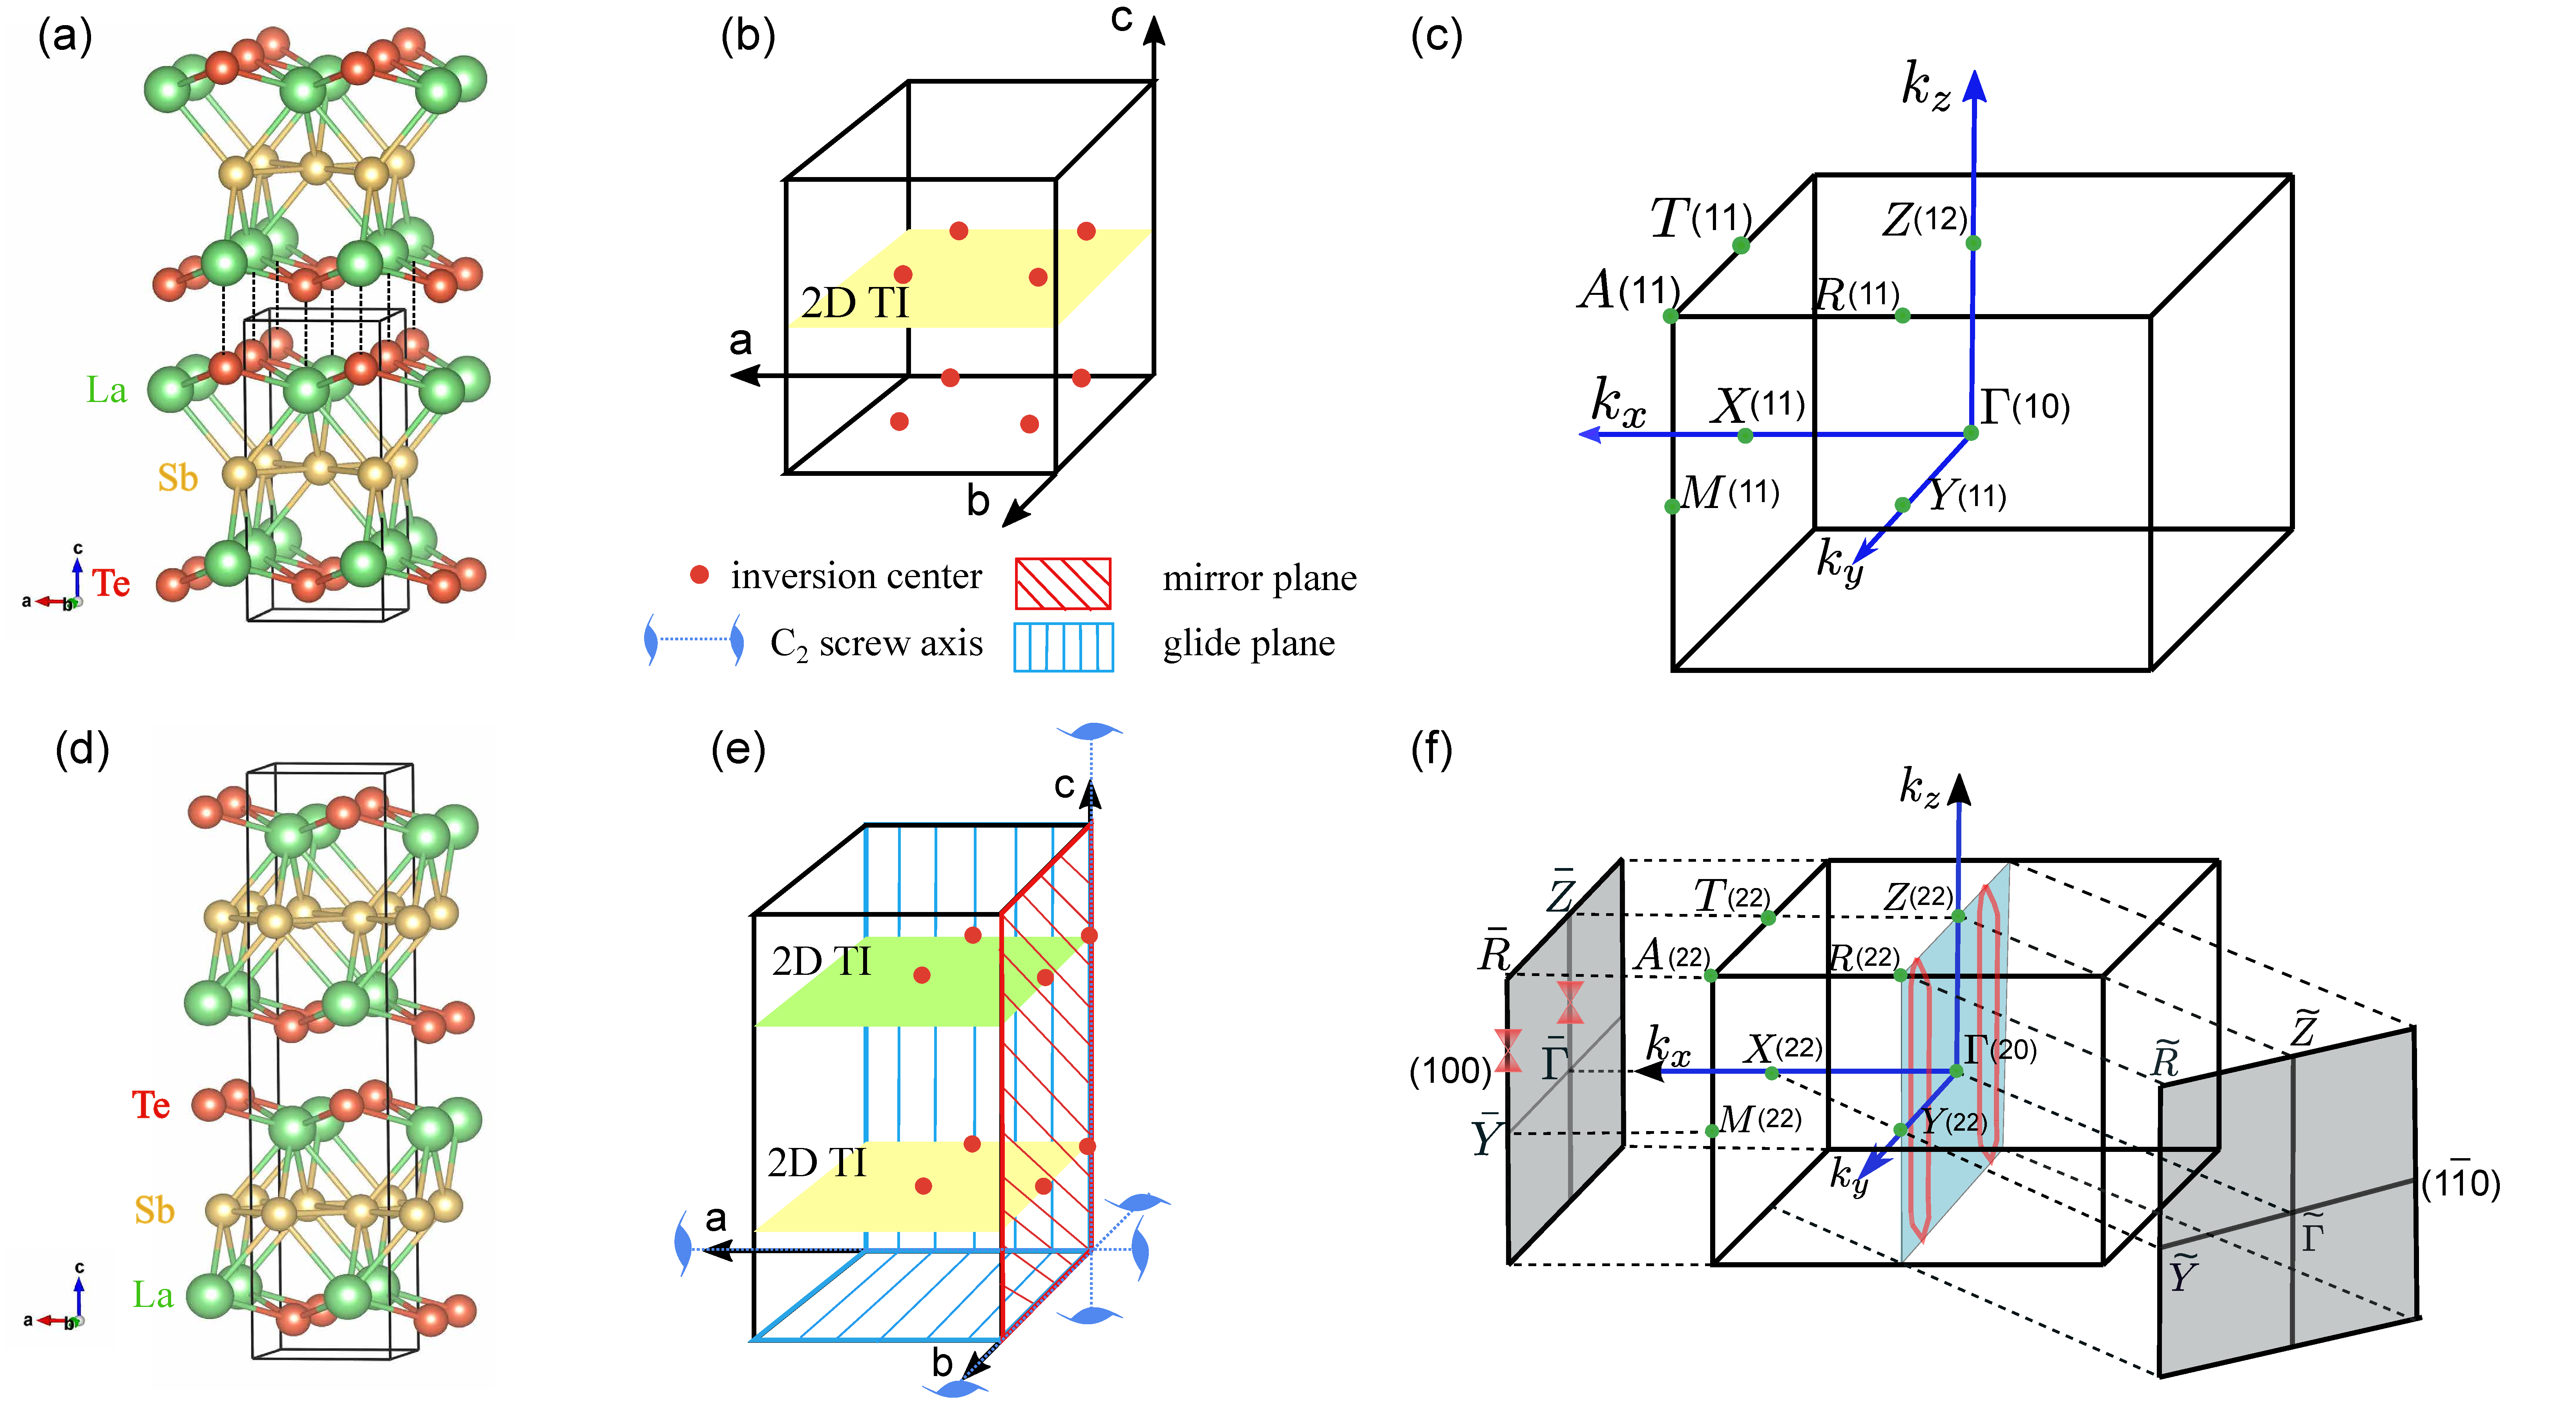
\includegraphics[width=0.9\textwidth]{lasbte-fig1.pdf}
    \bicaption{(a)$\tlasbte$的晶体结构。 
    (b)示意性地将弱拓扑绝缘体的层构造表示为对应于$\tlasbte$的晶格空间中2维拓扑绝缘体(黄色平面)的堆叠。 红色的点是反演中心。
    (c)$\tlasbte$的体布里渊区和高对称$k$点。$k$点旁边括号里的数值是占据态克拉默对中心反演操作本征值为负值的“对数”。
    (d)-(f)是$\olasbte$相应的信息。 
    在(e)中也标明了镜面,滑移面和螺旋轴。
    在图(f)蓝色的面代表镜面,躺在面内的红线代表没有考虑SOC时计算得到的节点环。灰色的面是$\olasbte$的(100)和(1$\bar1$0)面的表面布里渊区。其中,红色的沙漏型代表沿着相应路径上存在沙漏型的表面态。~\citep{qian2020layer}}
    {(a) Crystal structure for~\ti. (b) Schematically shows LC of a weak TI as the stacking of 2D TI (yellow plane) in lattice space corresponding to~\ti. The red dots are inversion centers.
    (c) The bulk BZ and high symmetrical crystal momenta for~\ti. The number in parentheses near high symmetrical momenta are the number of occupied Kramers pair bands with negative parity eigenvalues. (d)-(f) are for~\tci. In (e), the mirror plane, glide plane and screw axis are also shown. In (f) the blue plane indicates the mirror plane and the red lines inside of it represent the nodal rings calculated without including SOC. The dark grey planes are the projected surface BZ for (100) and (1$\bar 1$0) surfaces of~\tci,~where the red hourglass shapes represent the hourglass-like surface states along the two paths. ~\citep{qian2020layer}
    }
    \label{fig:3-1}
\end{figure}
%figure
{\it{晶体结构}}:LaSbTe有两个不同的晶体结构。一个是四方相$\tlasbte$,空间群是$P4/nmm$(No.129)。弛豫之后的晶格常数是$a=b=4.421$~\AA,$c=9.659$~\AA,和实验值 $a=b=4.44$~\AA, $c= 9.47$~\AA 相当。La和Te分别位于Wyckoff位置$2c$ $(0.5, 0.0, z)$,其中$z=0.7785$和$0.1282$。Sb在$2b$ $(0.0, 0.0, 0.5)$。$\tlasbte$是$MHM$家族之一,由沿着c轴五个原子层(QLs)重复堆叠而成,其中每五层按照[Te-La-Sb2-La-Te]序列排列。每个QLs之间的相互作用在图~\ref{fig:3-1}(a)中用虚线表示,这个相互作用比QLs内原子之间的相互作用要弱。
另一个相是正交相$\olasbte$,空间群是$Pmcn$ (No.62), 弛豫后的晶格常数是$a=4.422$~\AA, $b=4.433$~\AA, $c=19.348$~\AA。 实验的晶格常数是$a=4.378$~\AA, $b=4.403$~\AA,$c=19.242$~\AA。 La,Te和Sb分别位于Wyckoff位置$4c$ $(0.2500,0.2623,0.6106)$,$(0.2500,0.2614, 0.4360)$和$(0.2500,0.7283,0.2491)$。与$\tlasbte$相比,在$\olasbte$的每个原胞内有两个QLs,这可以有效地看作是由于每个QLs内Sb方格子层发生畸变,相邻的两个QLs内的Sb原子向相反方向移动导致QLs发生的二聚化。
$\olasbte$有中心反演对称性,一个镜面($m^{100}_{\frac{1}{2}00 }$),两个滑移面($g^{010}_{0\frac{1}{2}\frac{1}{2}}$, $g^{001}_{\frac{1}{2}\frac{1}{2}0}$)和三个二度螺旋轴($2^{100}_{ \frac{1}{2}0\frac{1}{2}}$, $2^{010}_{0 \frac{1}{2}0}$, $2^{001}_{\frac{1}{2}\frac{1}{2}\frac{1}{2}}$)。


这两个相结构的差异可以通过研究它们的声子谱,计算结果在图~\ref{phonon}(a,b)中显示。 $\olasbte$的声子谱计算表明它是一个稳定的相,而$\tlasbte$~的声子谱在$\Gamma$和$Z$点有虚频。在$Z$ (0, 0, 0.5)的软模表明加倍$c$轴会带来更稳定的晶体结构。如图~\ref{phonon} (c) 所示,这些软模主要来自Sb的振动模式,其中相邻两个QLs的Sb原子沿相反的方向运动。这使得Sb晶格面内不再是方格子而成为长方形,并且是如图~\ref{phonon} (d-f) 的俯视图和左视图所示的之字形结构。这样的晶格形变恰恰对应于从~$\tlasbte$~到~$\olasbte$的结构相变。
\ti~在$\Gamma$点的软模将导致晶体结构向11号空间群结构发生相变。相变到62号群结构在实验上已经发现,但是到11号群的相变目前为止还没有文献报道。
%figure
\begin{figure}[!htbp]
    \centering
    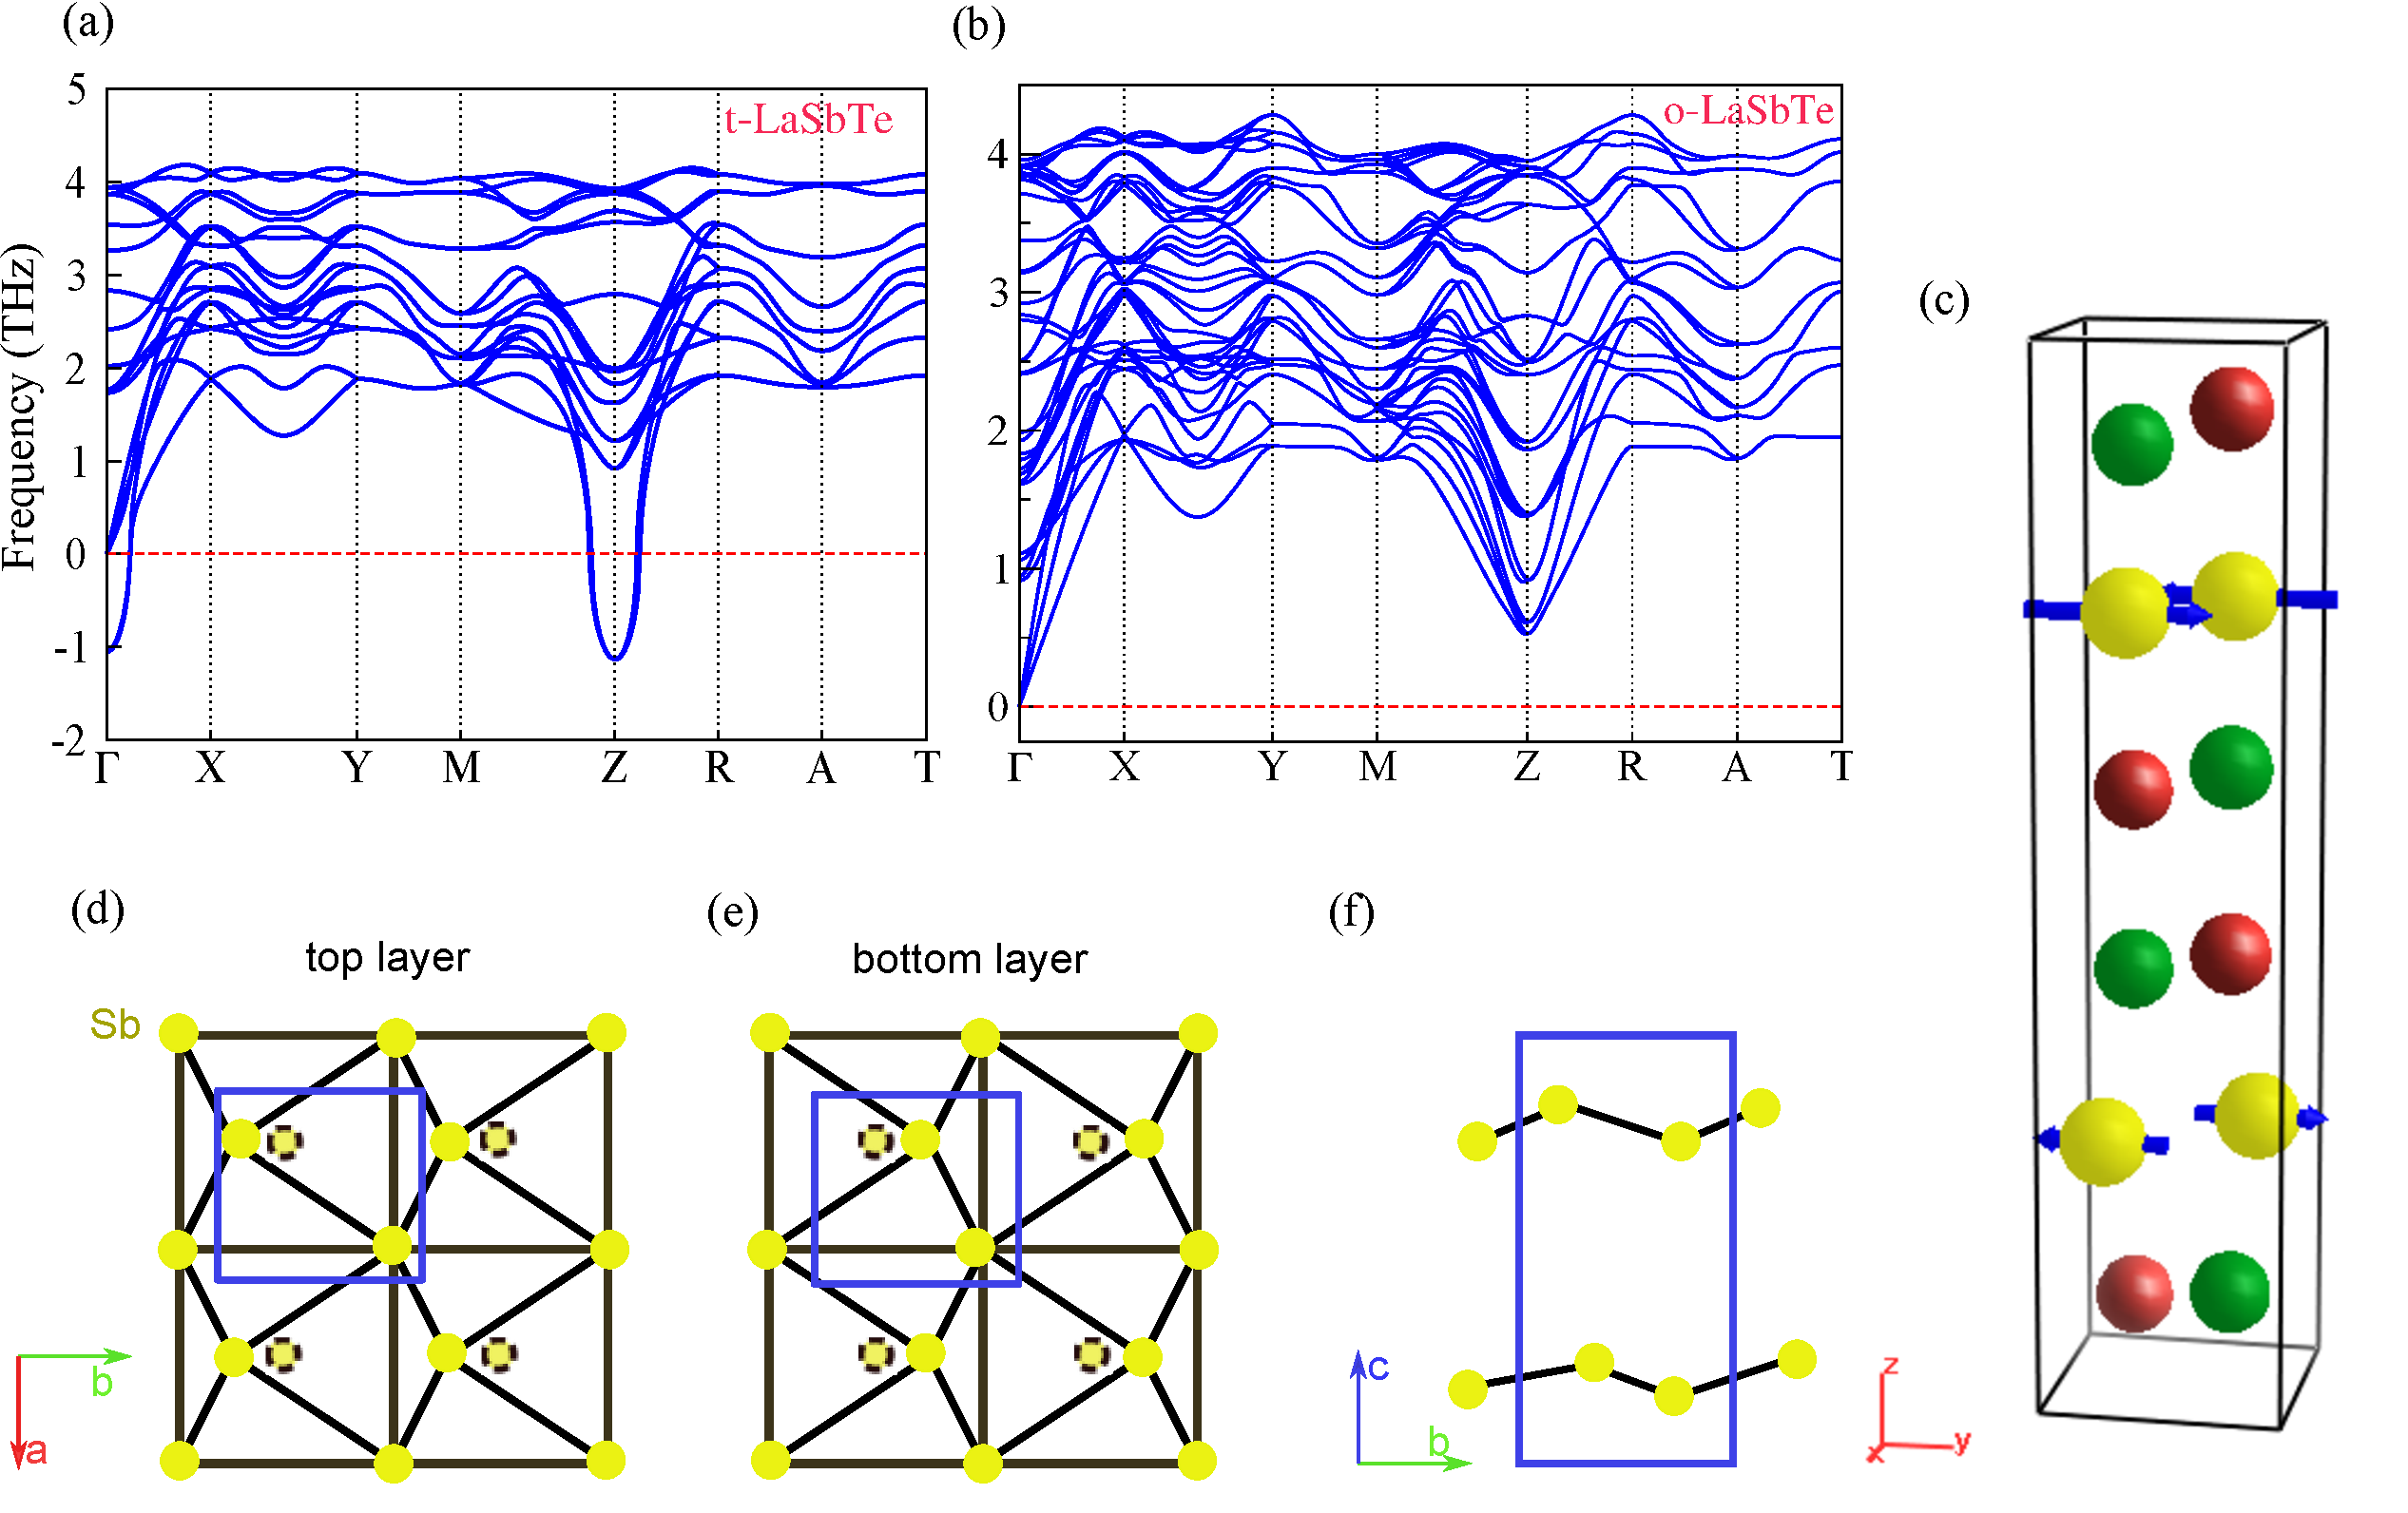
\includegraphics[width=14cm]{lasbte-fig2.pdf}
    \bicaption{(a)\ti 和(b)\tci 分别为计算得到的声子谱。(c)\ti 沿着c轴方向的两个原胞,在Sb原子上面的箭头标记$Z$点声子模式的振动方向。$4 \times 4 \times 1$的\tci 超胞(黑色框)沿着$c$的方向上面一层(d)和下面一层(f)Sb单层的示意图,其中蓝色的实框代表实际的原胞选取方法。红色的实心圆代表由\ti 中Sb原子(虚线的黄色圆)形变得到的\tci 中Sb原子,这与(c)中的软模一致。(f)\tci~沿$a$方向的侧视图展示了Sb原子沿着$b$轴之字形的链状结构。~\citep{qian2020layer}}
    {Calculated phonon spectra for (a) \ti~and (b) \tci , respectively. (c) Two unit cells of~\ti~along $c$-axis with arrows on Sb atoms denoting the displacement in one of the soft phonon modes at $Z$. The view from $c$-direction of the (d) top and (e) bottom Sb layer for a $4 \times 4 \times 1$ \tci~supercell (black box), the blue box represents the actual selection of the primitive cell. The solid yellow circle represents Sb atoms in \tci~due to distortion from those in \ti~(dotted yellow circles) consistent with the soft modes in (c). (f) The side view of \tci~from $a$-direction shows the zigzag chain like Sb atoms along $b$-axis. ~\citep{qian2020layer}}
    \label{phonon}
\end{figure}
%figure
\section{结果和讨论}
\subsection{电子能带结构}
%figure
\begin{figure}[!htb]
    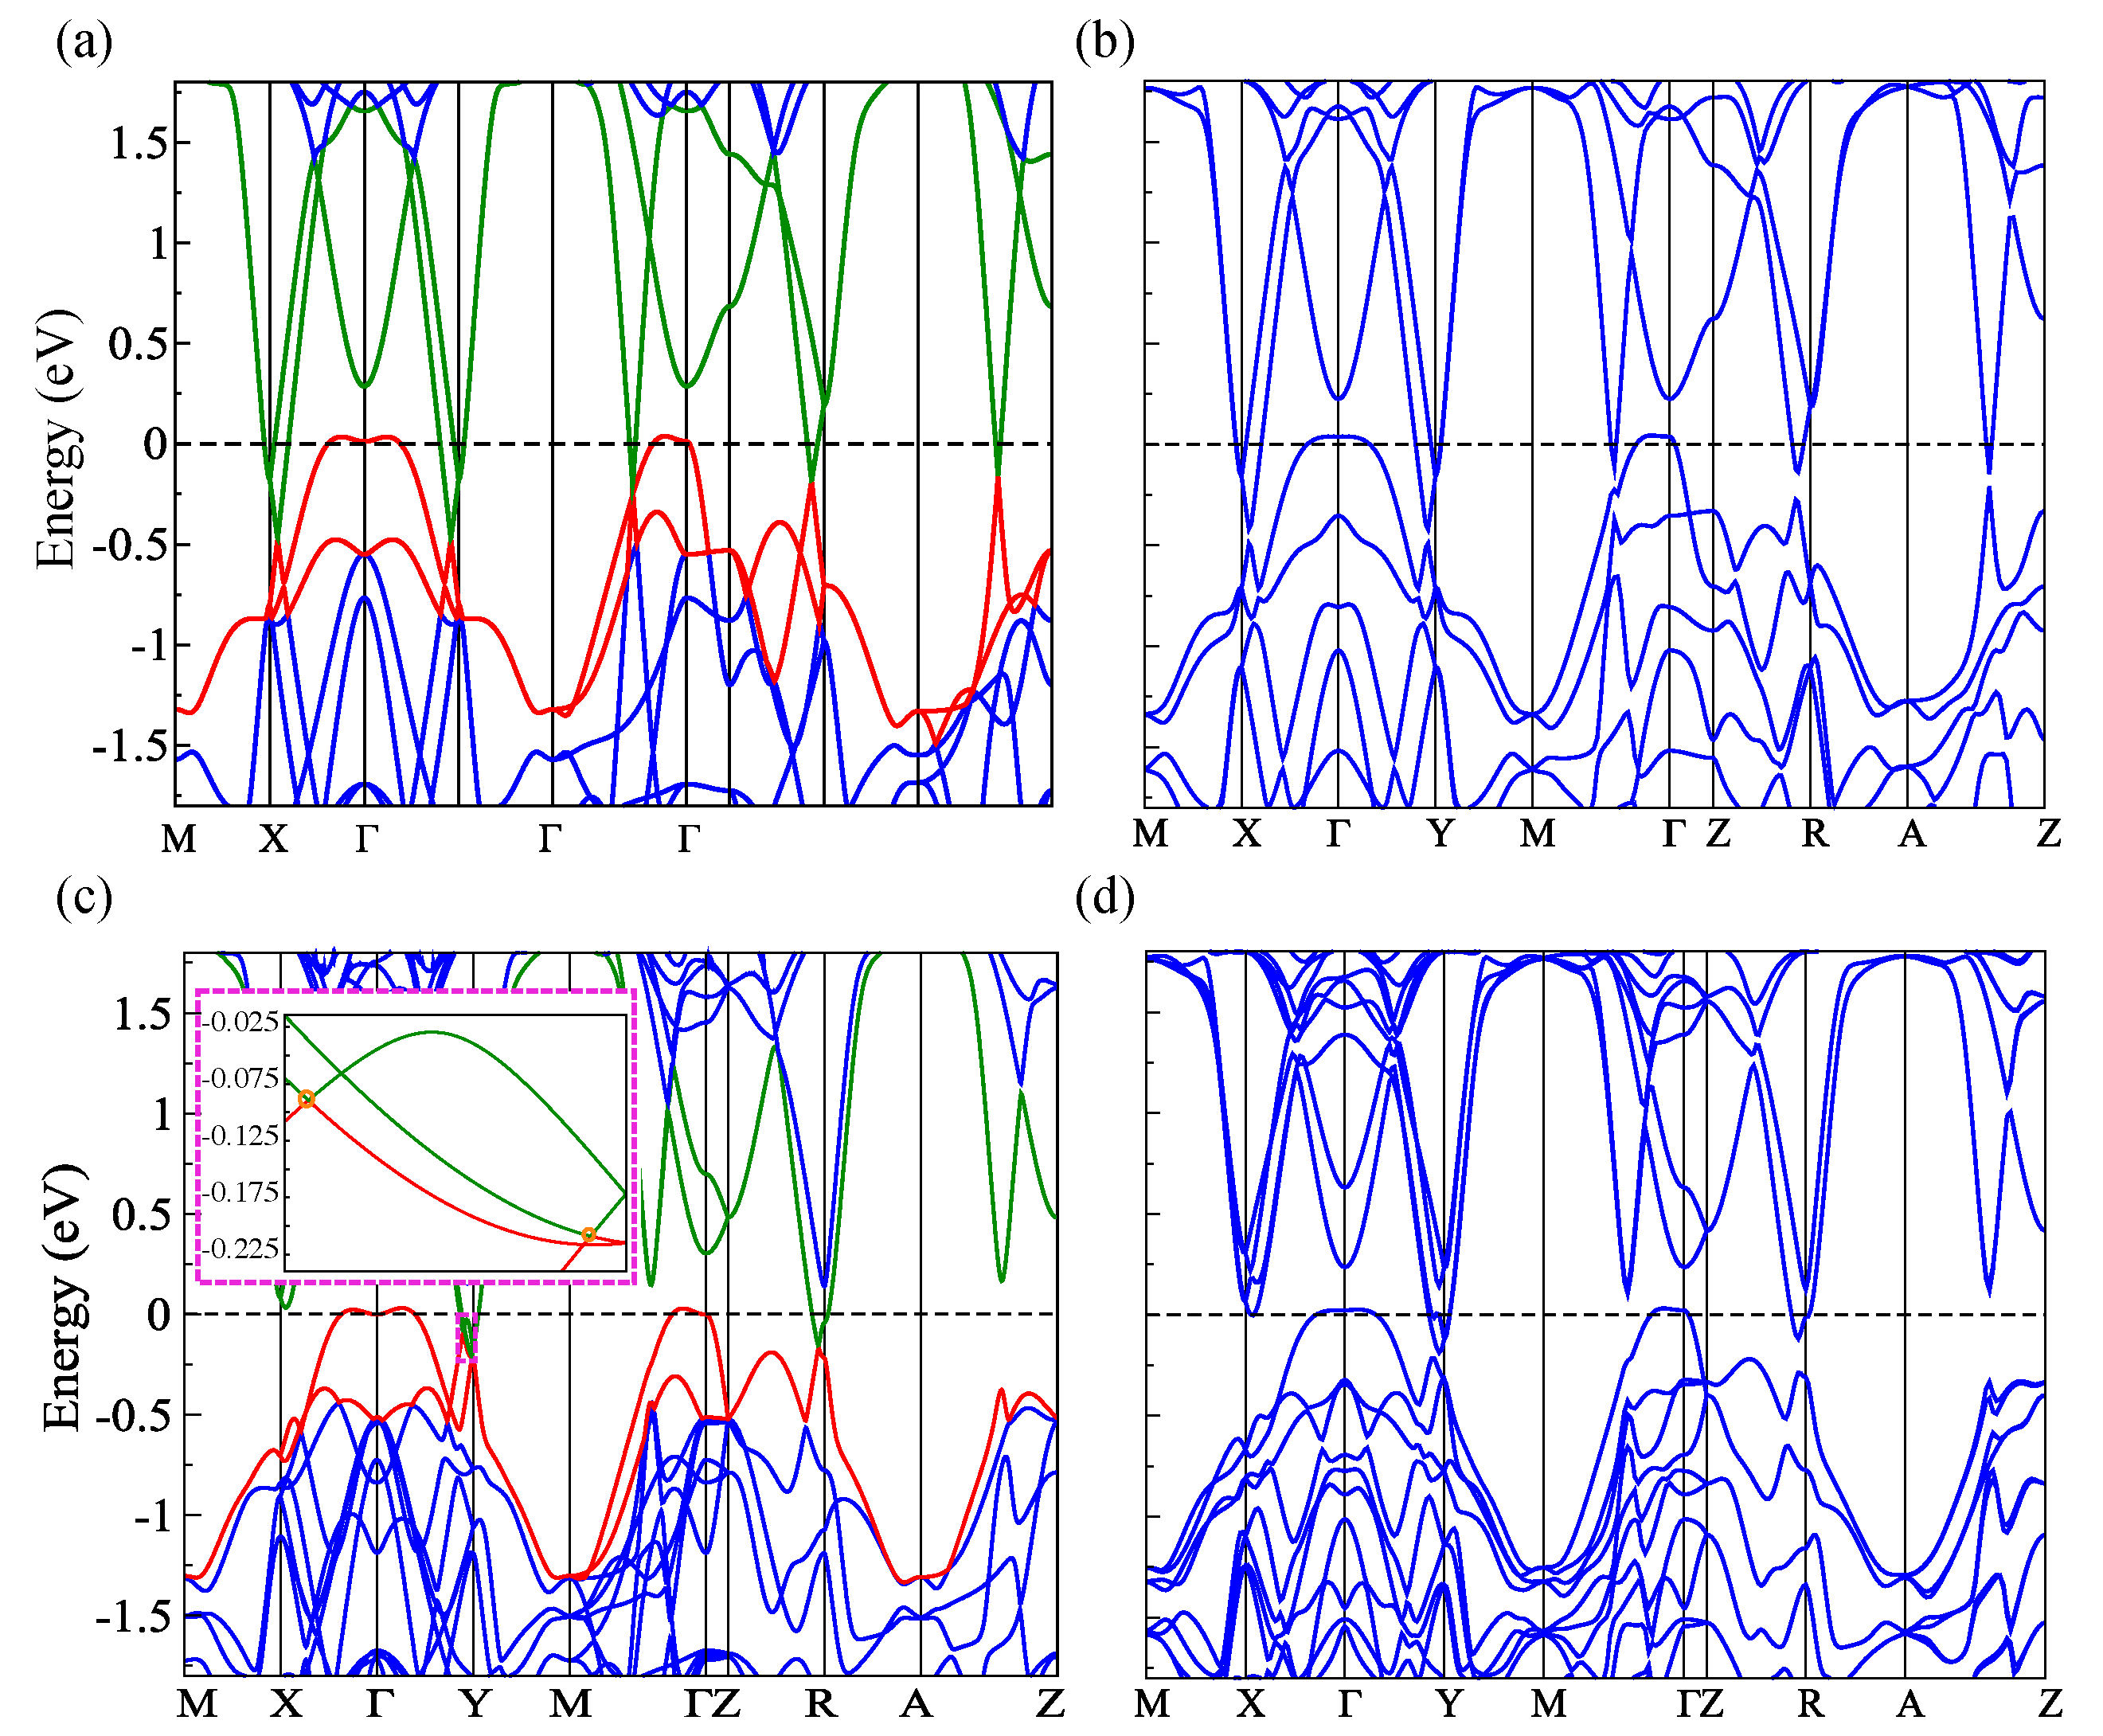
\includegraphics[width=1\textwidth]{lasbte-fig3.pdf}
    \bicaption{
    对 \ti~(a,c)和~\tci~(b,d)用GGA不考虑(a,b)和考虑(c,d)SOC时,沿着高对称线计算的能带结构。图(c)中的插图展示了不考虑SOC时沿着$\Gamma-$Y的能带反转。两条最高的价带和两条最低的导带分别用红色和绿色标记。~\citep{qian2020layer}
    }
    {
        Calculated band structures along the high-symmetry lines within GGA without (a, c) and with (b, d) SOC for~\ti~(a, b) and \tci~(c, d). The inset in (c) shows the band inversion feature along $\Gamma-$Y without SOC for \tci. The two highest valance bands and lowest conduction bands are marked in red and green, respectively. ~\citep{qian2020layer}
    }
    \label{fig:3-2}
\end{figure}
%figure

\ti~和~\tci~考虑和不考虑SOC的能带结构如图~\ref{fig:3-2}所示。众所周知,作为$WHM$家族的材料之一,在SOC忽略的情况下,\ti~有节点线结构~\citep{xu2015two, lou2016emergence}。 显而易见,在$k_z=0$的平面,沿着$\Gamma-X (Y)$和 $\Gamma-M$路径,在$k_z=\pi$平面,沿着$Z-R$,$Z-A$路径有能带交叉点。当SOC考虑进来时,所有节点线都打开带隙,从而使得\ti~成为弱拓扑绝缘体,按照QLs,即2维拓扑绝缘体的简单堆叠~\citep{xu2015two}。在不考虑SOC时,\tci~的能带结构也有交叉点,这些交点实际上是镜面$m^{100}_{\frac{1}{2}00 }$上节点线的一部分,如图\ref{fig:3-1}(f)所示。同时,SOC将使得节点线打开能隙,但会使得\tci~成为拓扑晶体绝缘体。


根据对称指标理论~\citep{nc_ashvin,wanxg2019},\ti~和~\tci~都有中心反演对称性,而且当考虑SOC时,他们的对称性指标为$\mathbb Z_{2,2,2,4}$,这个可以简单地通过类Fu-Kane公式得到~\citep{song2017, prx_ashvin}。三个弱拓扑指标$\mathbb Z_2$,标记为$z_{2w,i=1,2,3}$可以由以下公式计算得到:
%%equation%%%
\begin{equation}
\label{eq:1}
\begin{aligned}
z_{2w,i=1,2,3}\equiv&\sum_{\rm {\bold K}\in TRIM \;at \;\{k_i=\pi\}} n^{-}_{\bold K} \; \mathrm {mod} \;{2}
\end{aligned} .
\end{equation}
%%equation%%%

$\mathbb Z_4$指标记作$z_4$可由:
%%equation%%%
\begin{equation}
\label{eq:2}
\begin{aligned}
 z_4  \equiv \sum_{\rm \bold K \in TRIM} \frac {n^{-}_{\bold K} -n^{+}_{\bold K}}{2}  \; \mathrm {mod} \;{4}
 \end{aligned} ,
\end{equation}
%%equation%%%
获得,这里$n^{+}_{\bold K}$ ($n^{-}_{\bold K}$) 是时间反演不变点$\bold K$上占据态克拉默对有宇称为$+(-)$的数目。占据态克拉默对有宇称为负的数目已经在图~\ref{fig:3-1}中标出。 因此,根据方程~\ref{eq:1}和方程~\ref{eq:2},我们可以知道~\ti~有拓扑指标$\mathbb Z_{2,2,2,4}$为(0010)的弱拓扑绝缘体,而~\tci~是有拓扑指标为(0002)的拓扑绝缘体。我们知道每个单层,即~\ti~的QL是一个二维拓扑绝缘体~\citep{xu2015two}。在相变之后,形变的QL仍然是二维的拓扑绝缘体。在~\tci~原胞内是两个弱耦合的QLs的简单堆叠。这些不同之处和他们相应的拓扑不变量以及拓扑性质可以进一步通过层构造方案来理解,这个方法可以将实空间的晶体结构与倒空间能带拓扑联系起来。

\subsection{层构造和拓扑不变量}
直观上,\ti~可以看成是通过在密勒指数为(001; $\frac{1}{2}$)的平面上放置一层二维拓扑绝缘体来构造的。应用129号空间群所有的对称操作只能给出同样的密勒面。因此基本层构造eLC (001; $\frac{1}{2}$) 如图~\ref{fig:3-1} (b) 所示。在每个原胞内,这个eLC与$a$轴和$b$轴相交零次,和$c$轴相交一次,给出三个弱拓扑不变量$z_{2w, i=1, 2, 3}=0,0,1$。eLC (001; $\frac{1}{2}$) 占据8个反演中心中的四个,这意味着对于这个eLC由中心反演对称性保护的拓扑不变量$\delta_i$是规范依赖的,所以$z_4=0$, $\delta_i=0$。这个eLC不占据任何旋转轴,螺旋轴,镜面或者滑移面。并且,对于螺旋和滑移操作,它不给出任何非零的堆叠不变量。这意味旋转,螺旋,镜面和滑移所对应的拓扑不变量都是零,因此~\ti~是弱拓扑绝缘体而不是拓扑晶体绝缘体。

从~\ti~到~\tci~的结构相变已经通过~\ti~在$Z$点的软模表明。这导致结构沿着$c$轴的加倍和原子的移动。因此在~\tci~的原胞有两个二维拓扑绝缘体,位于密勒面 (001; $\frac{1}{4}$) 和 (001; $\frac{3}{4}$) 。这两个二维拓扑绝缘体构成62号群的一个eLC (001; $\frac{1}{4}$) 或者eLC  (001; $\frac{3}{4}$) 。在本文所选择的规范下,这两个层与三个晶格矢量相交偶数次,所以$z_{2w, i=1, 2, 3}=0$。在图~\ref{fig:3-1} (e) 中所有的反演中心都被这两个二维拓扑绝缘体占据了, 这表明$\delta_i=1$,$z_4=2$。同样地,这个eLC不占据任何镜面和滑移面,也不穿过任何旋转轴。但是,滑移面 $g^{010}_{0\frac{1}{2}\frac{1}{2}}$和螺旋轴 $2^{100}_{ \frac{1}{2}0\frac{1}{2}}$,$2^{001}_{\frac{1}{2}\frac{1}{2}\frac{1}{2}}$会贡献非零的堆叠不变量。所以,相应的拓扑滑移不变量$\delta_h$和螺旋不变量$\delta_s$等于1。通过这个方法,~\tci~的时间反演对称和晶体对称性所保护的拓扑态都被完全确定下来了。它是一个拓扑晶体绝缘体,相应的对称性指标为$\mathbb Z_{2,2,2,4}=(0002)$,拓扑不变量为  $\delta_i=1$, $\delta_{h}^{(010)}=1$和$\delta_{s}^{(100)}=\delta_{s}^{(001)}=1$。
 

\subsection{从拓扑不变量到拓扑表面态}

\begin{figure*}[!htb]
\centering
\includegraphics[width=15 cm]{lasbte-fig4.pdf}
\bicaption{
在(100)(a-c)和(1$\bar 1$0)(d-f)表面的Wilson loop谱和表面态能带结构。(b, e)分别是(a)和(d)阴影部分的放大。可以很清楚的看到在(b,c)中有沙漏型的拓扑表面态,但是(e, f)中有开能隙的平庸的表面态。~\citep{qian2020layer}
}
{
The spectra of Wilson loop and SS band structures on surface BZ of (100) (a-c) and (1$\bar 1$0) (d-f) surfaces, respectively. (b, e) The zoomed in image of the shadowed part in (a) and (d), respectively. It can be seen clearly that there are hourglass-like SSs in (b, c) but trivial SSs with full gap in (e, f). ~\citep{qian2020layer}
}
\label{fig:3-4}
\end{figure*}

不平庸的滑移不变量$\delta_h$表明存在不平庸的沙漏型拓扑表面态在保持相应的滑移对称性的表面上~\citep{wang2016hourglass,bernevigprx}。
我们知道,定义在布里渊区占据态纤维丛上的Wilson loop谱同构于表面态能谱~\citep{fidkowski2011model}。我们可以通过计算体态哈密顿量Wilson loop谱或者计算截断表面作为边界条件的表面格林函数得到表面态,来验证滑移不变量的正确性。~\citep{WU2017,Sancho_1985}。
在(100)表面,由于滑移对称性$g^{010}_{0\frac{1}{2}\frac{1}{2}}$保持并且投影到$\bar\Gamma-\bar Z$和$\bar R-\bar Y$路径,滑移不变量$\delta_{h}^{(010)}=1$可以保护不平庸的沙漏型表面存在,如图~\ref{fig:3-1}(f)所示。
在~\ref{fig:3-4} (a)和(b)中,Wilson loop谱清楚地显示$\bar\Gamma-\bar Z$ and $\bar R-\bar Y$有沙漏型的表面态。而且两个沙漏型表面态之间$\bar Z-\bar R$路径的连接曲线有一般的锯齿形图案,表现出谱状结构~\citep{bernevigprx}。通过格林函数方法计算表面态,我们发现沿着$\bar\Gamma-\bar Z$路径可以清晰地看到沙漏型的表面态,如图~\ref{fig:3-4}(c)所示。但是,沿着$\bar R-\bar Y$的表面态由于混合到体态中很难被看到。
类似地,不变量$\delta_{h}^{(001)}$是平庸的,所以在(1$\bar1$0)表面,当投影到$\tilde Z-\tilde R$和$\tilde Y-\tilde\Gamma$方向(保持$g^{001}_{\frac{1}{2} \frac{1}{2} 0 }$对称性)时,应该有平庸的表面态。
在图~\ref{fig:3-4}(d, e)中沿着$\tilde Z-\tilde R$ 和 $\tilde Y-\tilde\Gamma$方向,沙漏型的表面态其实是平庸的。因为当在整个表面布里渊区沿着$\tilde Z\tilde R\tilde Y\tilde\Gamma$看,他们之间的连接方式在谱线上有明显的能隙,表现出各自孤立的状态,这和图~\ref{fig:3-4}(f)中拓扑平庸的表面态计算结果相吻合。

不平庸的滑移不变量$\delta_s$可以保护棱态,这些已经在很多工作中~\citep{wang2016hourglass,Fangc2t,zhangt2019}被详细讨论过,在此为了简洁起见将不再赘述。


\section{结论}
基于第一性原理计算,我们发现拓扑晶体绝缘体相\tci~有沙漏型的表面态和棱态,可以看作是两个\ti~由于结构相变而来。这种维度降低的方法可以有效的抓住拓扑晶体绝缘体的物理本质。 
特别是据我们所知道,这是第一次找到一个实验可以得到的材料能够生动形象地将实空间的层构造和动量空间的能带拓扑相对应。例如对于拓扑晶体绝缘体家族 Ba$_3$Cd$_2$As$_4$ \citep{zhangt2019}也可以看作是由层构造: $(001;0){\otimes} (001;\frac{1}{2})$得到,但是这个层构造不能直接对应于实空间的晶体结构。所以这个完美的例子为我们理解拓扑晶体绝缘体和拓扑绝缘体的关系和物理本质提供了非常好的平台。
\chapter{具有{S$_4$}对称性的外尔半金属}\label{chap:s4}

在破缺时间反演对称性但保持中心反演对称性的体系中,外尔点的出现可以由在八个中心反演不变点奇数条偶宇称/奇宇称占据态能带来保证。在这里,基于对称性分析和第一性原理计算,我们证明了对于有$S_4$的时间反演不变的体系,外尔半金属相可以由两个可以很好定义的不相等的不变量 $\eta$ 和$S_4$指标$z_2$来判断。
通过应用这个判据,我们发现一些之前认为是在非中心对称但有$S_4$对称性的空间群里发现的拓扑绝缘体的材料实际上是外尔半金属。
我们的第一性原理计算表明在有四对外尔点出现在$k_{x,y}$ = 0面,每个平面包含四个手性相同的外尔点。我们建立了有效模型来理解这些材料拓扑不平庸的本质。我们使用对称性指标和拓扑不变量的方法在对于时间反演不变的体系内寻找外尔半金属开辟了一条新的路径。 

\section{背景}
在过去的几十年,拓扑材料吸引了很多研究者的兴趣~\citep{bernevig2006quantum,zhang2009topological,Qi2010The,TIreview, Wan2011,wang2013three,Weng2016Topological,wang2016hourglass,PRBwzj,pre96wang,tqc2017,RevModPhys.90.015001,prb97wang}。许多拓扑绝缘体的候选材料首先被理论预言,后来又被实验证实~\citep{bernevig2006quantum, konig2007quantum, zhang2009topological, chen2009experimental, advwang}。大多数的预言都是通过拓扑不变量或者对称性指标来判断的~\citep{Fu2007topo, Fu2007IS,Slager2017, haruki2018, song2017, Vergniory2019, Zhang2018, wanxg2019}。拓扑外尔半金属~\citep{Murakami_2007,Liu2014Weyl,weng2015weyl,soluyanov2015type,lv2015observation,lv2015experimental,Weng2016Coexistence,PhysRevLett.117.236401,nie2017topological,sakai2018,prb99} 在具体的两重简并点附近有线性的色散。这个两重简并点被称为外尔点,它可以看作是动量空间贝利曲率的漏或源。他们表现出许多新奇的性质,比如在表面上的费米弧~\citep{Wan2011,xu2015discovery,xu2016observation,wang2016observation2},手性反常~\citep{huang2015observation,zhang2016signatures}, 和量子反常霍尔效应~\citep{Fang92,xu2011chern}等。但是,因为在三维空间外尔点不需要任何具体的对称性保护(除了平移对称性外),所以时间反演不变的(TRI)系统里的外尔半金属通常不能基于拓扑不变量和对称性指标来预测。据我们所知,对于时间反演对称性破缺(TRB)的中心对称体系,在中心反演不变的(ISI)动量上有奇数个偶/奇宇称占据态的能带可以保证外尔点的出现~\citep{Hughes2010Inversion,PhysRevLett.117.236401,nie2019magnetic}。这可以简单的通过两个平行的空间反演不变的平面上不等价的陈数(如果可以很好的定义)来简单的理解,如图~\ref{fig:5-1}(a) 和 \ref{fig:5-1}(b)所示。 在这里,我们的目的就是去找到可以保证外尔半金属相的合适的拓扑不变量或者定义在时间反演平面上的对称性指标。

\begin{figure}[!tb]
    \centering
    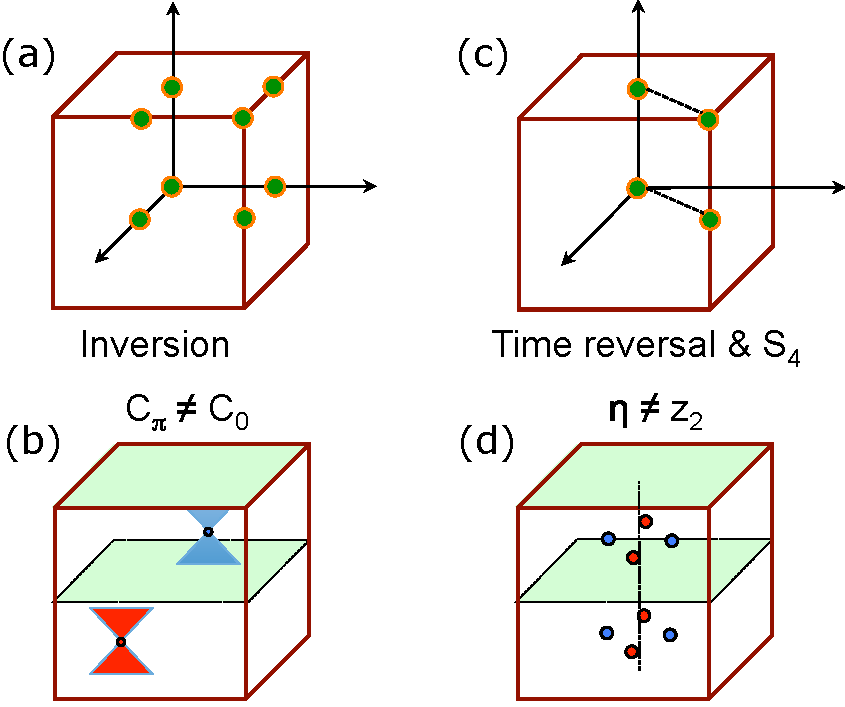
\includegraphics[width=9.2 cm]{s4-fig1.pdf}
    \bicaption{
        示意地展示具有对称指标和拓扑不变量的外尔半金属。
        对于时间反演对称性破缺的中心对称体系,在中心反演不变的动量 [(a)中绿色点 ] 上有奇数个偶/奇宇称占据态的能带,代表两个中心反演不变的平面的陈数是不同的(b),这可以保证3维布里渊区内有奇数对外尔点出现。注意,在时间反演不变的系统,偶/奇宇称占据态的能带数目总是偶数。对于具有时间反演不变和$S_4$对称性的系统,可以在四个$S_4$不变点[图(c)绿色点]的定义一个$z_2$指标,而且不变量$\eta$ [ 定义在正文内 ] 和$S_4~z_2$指标的不相等表明有外尔点出现,如图(d)。
        红色(蓝色)点代表+1(-1)手性的外尔点。~\citep{Qians4}
        } 
        {Schematic WSMs with symmetry indicators and topological invariants.
        For a TRB centrosymmetric system, an odd number of even/odd parity occupied bands at eight ISI momenta [green dots in (a)] reveals that the Chern numbers of the two ISI planes are different, which guarantee the appearance of odd pairs of Weyl points in 3D Brillouin zone (BZ) (b). Note that there is always an even number of even/odd parity occupied bands in a TRI system.
        For a TRI and $S_4$-symmetric system, a $z_2$ indicator is defined on four $S_4$ invariant momenta [green dots in (c)], and the inequality between the invariant $\eta$ [defined in the main text] and $S_4~z_2$ indicator reveals the appearance of Weyl points, as shown in (d). The red (blue) dots stand for +1 (-1) chiral Weyl points. ~\citep{Qians4}
    } 
    \label{fig:5-1}
\end{figure}

在这个工作中,我们主要关注有$S_4$对称性的时间反演不变的系统 (关于$S_4$不变的系统更一般的讨论可以参考文献~\citep{tobedone2019}) 。
在这些系统里,我们定义一个拓扑不变量$\eta$:
\begin{equation*}
(-1)^{\eta}=(-1)^{\nu_{a_1}}(-1)^{\nu_{a_2}},
\end{equation*}
只要有两个平行的完全开能隙的时间反演不变的平面(例如, $a_1$-面和$a_2$-面),这个不变量就可以很好的定义。不变量$\nu_{a_1}$ 和 $\nu_{a_2}$是两个平行的时间反演不变的平面内的时间反演不变的$\mathbb Z_2$不变量~\citep{Kane2005}。
此外,$ S_4 $对称性定义了对称性指示符$z_2$~\citep{song2017,haruki2018}。
注意,如果两个对称性指标都可以很好定义的话,在中心对称的时间反演不变的系统他们总是满足$\eta=z_2$~\citep{Fu2007topo,haruki2018}。这里,我们发现$\eta$ 和 $z_2$ 不相等意味着一般有外尔点出现(不考虑额外对称性)。具体来说,如果材料满足$\eta\neq z_2$则是外尔半金属,如图~\ref{fig:5-1} (b) 和~\ref{fig:5-1} (d) 。


%Fortunately, we find that it can be  the difference between three topological invariants [$\eta_i \equiv |{\mathbb Z}_{2,k_i=0}-{\mathbb Z}_{2,k_i=\pi}|,~i\in\{1,2,3\}$], where ${\mathbb Z}_{2,k_i=0(\pi)}$ is the TR $\mathbb Z_2$ invariant in the $k_i=0(\pi)$ plane and $k_{i=1,2,3}$ are along the directions of three primitive reciprocal lattice vectors. We note that the insulating phase has to satisfy the equivalence: $\eta_1=\eta_2=\eta_3$. It's also notable that a centrosymmetric system always satisfies the equivalence as long as the system is fully gapped.  Therefore, a system which does {\emph not} satisfy that equivalence can be a Weyl semimetal in general.  If we further consider S$_4$ symmetry, which defines another $\mathbb Z_2$ indicator ($z_2$), the equivalence that the insulating phase satisfies reduces to $\eta_z=z_2$.
许多年前,121号群 ($I\bar 42m$) 非中心对称的结构中的许多化合物被认为是拓扑绝缘体 ~\citep{Wang2010}。但是,我们仔细研究后发现,基于$S_4$对称性指标,这些所谓的“拓扑绝缘体”(``TIs")实际上可以分为两个不同的情况: $z_2=1$ (\tii~) 和 $z_2=0$ (\wsm~) 。
在这个工作,我们证明在\wsm~中的``TIs"实际上是外尔半金属。在$k_{x,y}=0$ 面上发现四对外尔点,每个平面包含四个手性相同的外尔点。此外,外尔点正好位于电荷中性能级。$\eta$ 和 $z_2$  (即, $\eta\neq z_2$) 可以来判别外尔半金属,这个方法也可以应用于其他具有$S_4$对称性的空间群~\citep{Haijun2016,HgTenc2016}。为了抓住121号空间群拓扑不平庸的物理本质,我们构造了六带低能有效模型。也给出了作为外尔半金属的标志的费米弧表面态。我们通过使用对称性指标和不变量找到外尔点的策略,开辟了一条在时间反演不变系统中搜索外尔半金属的新途径。


%We find that, in general, the Weyl semimetal phase with time-reversal symmetry is characterized by the difference between three topological invariants ($\eta_i \equiv |{\mathbb Z}_{2,k_i=0}-{\mathbb Z}_{2,k_i=\pi}|,~i\in\{1,2,3\}$), where ${\mathbb Z}_{2,k_i=0(\pi)}$ is the $\mathbb Z_2$ invariant in the $k_i=0(\pi)$ plane and $k_{i=1,2,3}$ are three primitive reciprocal lattice vectors.

%The difference between the $S_{4z}$ indicator ($\mathbb Z_{2,S_{4z}}$) of the two phases in these topological compounds intrigues us to investigate them further. These topological insulators have shared same TR $\mathbb Z_2$ invariants in the $k_z=0$ and $k_z=\pi$ planes: $\mathbb Z_{2,kz=0}=1$ and  $\mathbb Z_{2,kz=\pi}=0$, which is






\section{晶体结构和计算方法}
%Yuting,  Please fill it up with the description of crystal structures and Methodology.
%\emph{Crystal structure and Methodology.} -- 
{\it{晶体结构}}: 我们研究了锡矿结构中的一系列铜基硫族元素化物:Cu$_2$-Cu-Sb-VI$_4$ 和 Cu$_2$-II-IV-VI$_4$,其中 II=$\{$Cd, Hg, 和 Zn$\}$, IV=$\{$Si, Ge, 和 Sn$\}$, 和 VI=$\{$S, Se, 和 Te$\}$。这一系列化合物是空间群$I \bar 4 2 m$ ($D_{2d} $),体心四方结构,晶格常数为: $a$ 和 $c$。
% Among these compounds, we take Cu$_2$ZnGeSe$_4$ as an example for WSM and \ti for TI, respectively. More results on other compounds are presented in the Supplemental Material (SM).  Here we take Cu$_2$ZnGeSe$_4$ as an example .
这个结构有三个2度旋转轴($C_{2x,2y,2z}$), 两个镜面对称性 ($M_{xy,\bar xy}$),有时间反演对称 ($I$) 和四重旋转对称 ($C_{4z}$) 的组合对称操作 S$_4$,但是没有单独的 $I$ 和 $C_{4z}$。
在图~\ref{fig:5-2} (a) 展示了呈现锡矿结构。
每个阴离子均通过具有三个不等价键的四个阳离子进行四面体配位:VI-Cu,VI-II和VI-IV。
晶体结构沿$ c $轴几乎是二倍的闪锌矿结构,但由于层间耦合而具有以$c\neq2a$为特征的变形。这些化合物代表应变后的HgTe类材料~\citep{HgTenc2016}。

\begin{figure}[!tb]
\centering
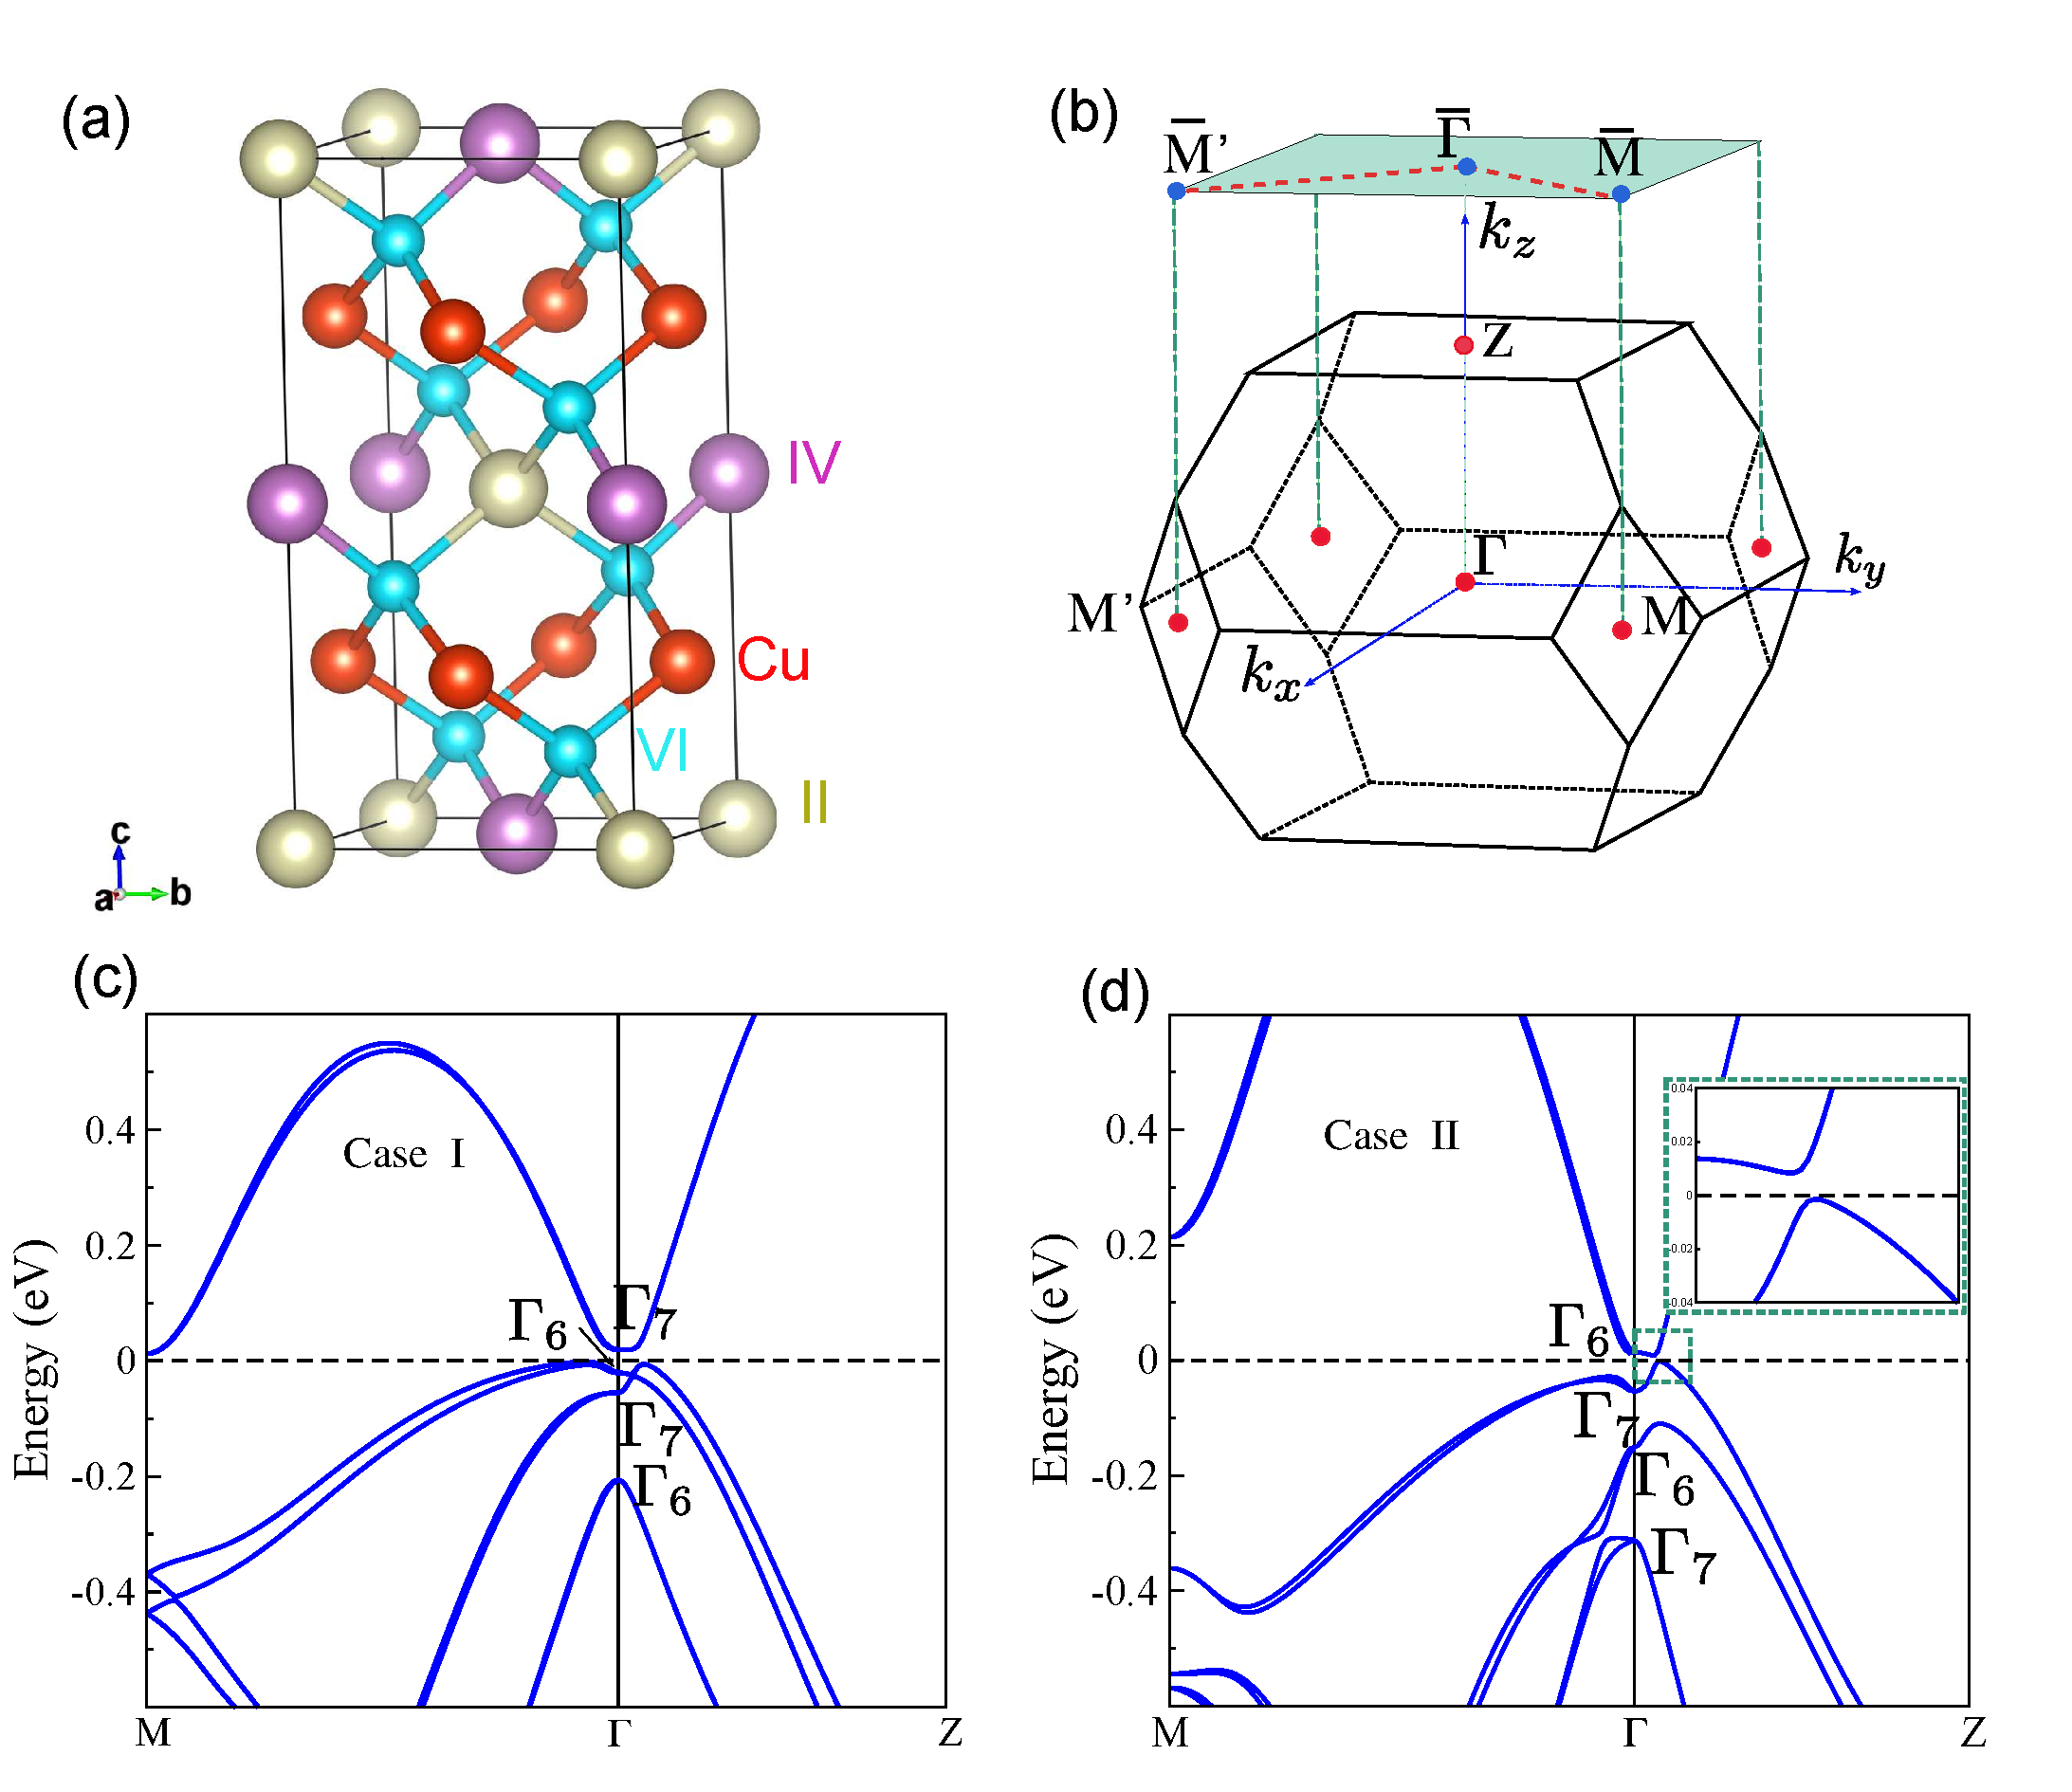
\includegraphics[width=8.5 cm]{s4-fig2.pdf}
\bicaption{
    (a)四元锡矿物Cu$_2$-II-IV-VI$_4$的晶体结构和(b)系列121空间群化合物的布里渊区。有混合的II和IV原子的交替阳离子层,它们通过Cu一价阳离子层相互分隔。两个等价的Cu原子, 一个II原子, 一个IV原子和四个VI原子分别占据$4d$, $2a$, $2b$ 和 $8i$ Wyckoff位置。在Cu$_2$-Cu-Sb-VI$_4$结构里, $2a$ 和 $2b$ 位置分别由Cu 和 Sb 原子占据。
    分别对\tii~和\wsm~给出了(c)\tic~和(d)\wsmc~的考虑SOC时的电子能带结构和$\Gamma$点的不可约表示。~\citep{Qians4}}
    {
    (a) Crystal structure of the quaternary stannite Cu$_2$-II-IV-VI$_4$ compounds and (b) BZ for the series of compounds in space group 121. There are alternating cation layers of mixed II and IV atoms, which are separated from each other by layers of Cu monovalent cations. Two equivalent Cu atoms, one II atom, one IV atom and four VI atoms occupy the $4d$, $2a$, $2b$ and $8i$ Wyckoff positions, respectively. In the Cu$_2$-Cu-Sb-VI$_4$ structure, the $2a$ and $2b$ positions are occupied by Cu and Sb atoms, respectively.
    The electronic band structures and irreps at $\Gamma$ point with SOC for (c) \tic~and (d) \wsmc~are presented for \tii~ and \wsm, respectively. ~\citep{Qians4}
    } \label{fig:5-2}
\end{figure}


{\it{计算方法}}: 
我们使用基于密度泛函理论的缀加平面波方法\citep{paw1,paw2}的VASP软件包\citep{KRESSE199615,vasp}进行第一性原理计算。
 %were employed in our first-principles calculations.
 交换关联泛函选取GGA的PBE泛函~\citep{pbe}。平面波的动能截断为400 eV。自洽计算过程对布里渊区取样为10$\times$10 $\times$10 $k$网格。晶体结构和原子参数来自Inorganic Crystal Structure Database (ICSD),展示在表格~\ref{tab:5-s1}。计算了考虑自旋轨道耦合(SOC)的电子能带结构。采用Wilson-loop方法~\citep{Yu2011An}计算拓扑不变量和手性电荷~\citep{Fang92}。


\section{结果和讨论}
\subsection{电子能带结构}
\begin{figure*}[!htb]
    \centering
    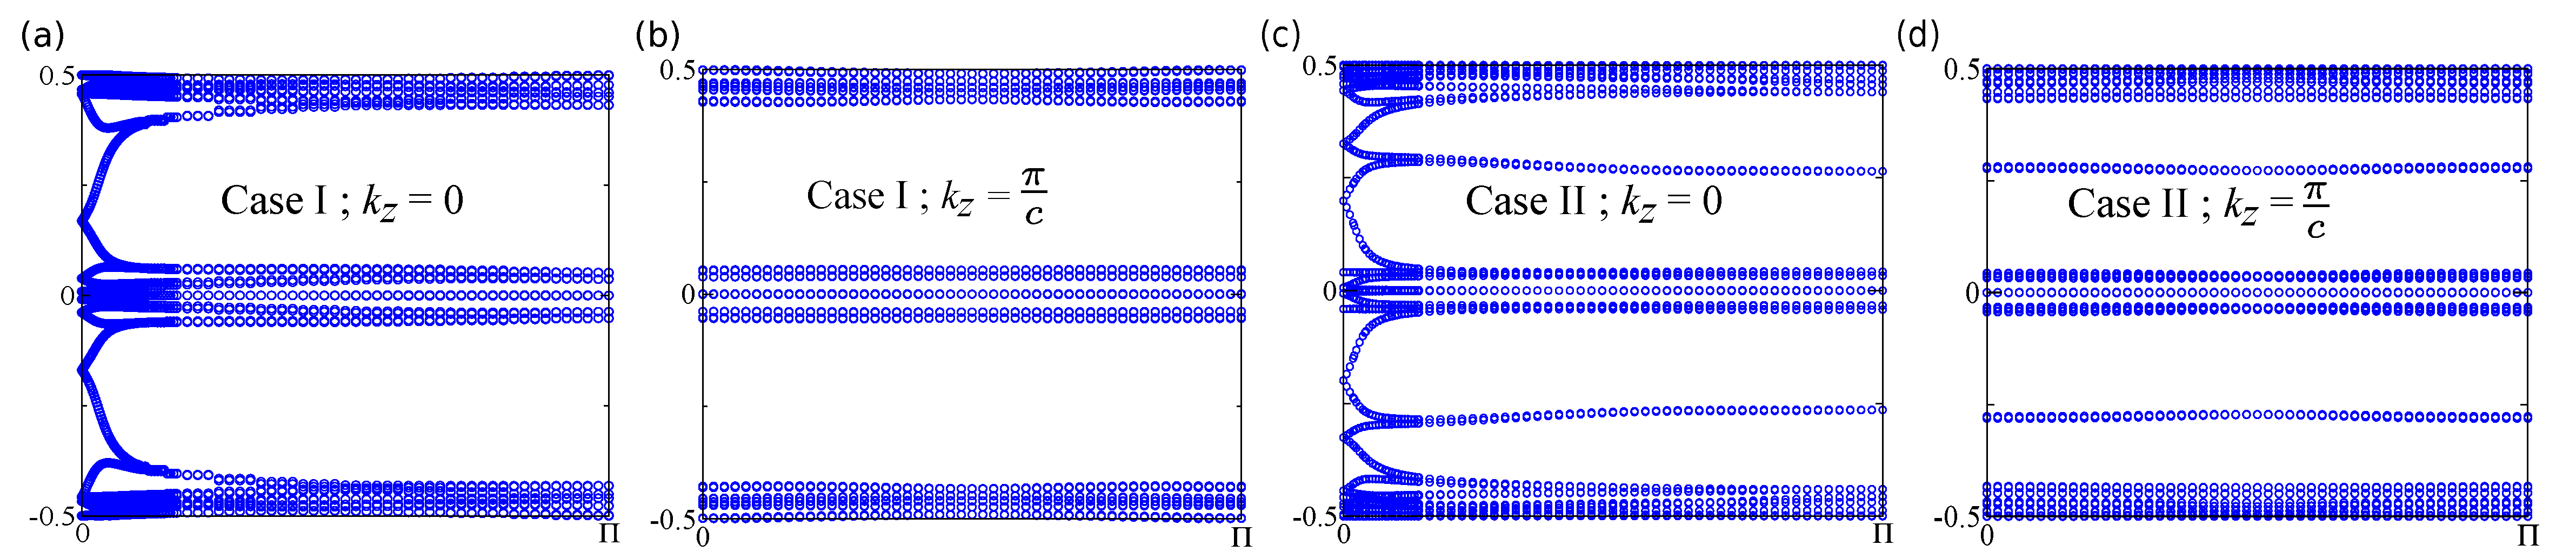
\includegraphics[height=3.2cm]{s4-fig4z2.pdf}
    \bicaption{
    (a, b)和(c, d)分别为\tii~和\wsm~在$k_z=0$ 和 $k_z={\frac{\pi}{c}}$平面上时间反演$\mathbb Z_2$的计算结果。~\citep{Qians4}
    }{
    The calculated time-reversal $\mathbb Z_2$ in  $k_z=0$ and $k_z={\frac{\pi}{c}}$ planes for \tii~ (a, b) and \wsm~ (c, d), respectively. ~\citep{Qians4}
    } \label{fig:5-s2}
    \end{figure*}
    
基于第一性原理计算,我们对先前工作中认为拓扑绝缘体的一类材料的能带结构重新进行了研究~\citep{Wang2010}。
我们发现这些化合物其实可以分为两类。在文章中,我们将\tic~(\tii) 和 \wsmc~(\wsm) 化合物分别作为这两种情况的例子,沿着高对称线上计算得到的能带结构如图~\ref{fig:5-2}。其他化合物的能带结果如图~\ref{fig:5-s1},这里使用的是ICSD报道的实验的晶格常数[如表~\ref{tab:5-s1}].
%qianyt
%For the series of the compounds in space group 121, we have systematically computed band structures and time-reversal $\mathbb Z_2$ invariants in the two planes: $k_z=0$ and $k_z=\frac{\pi}{c}$ as shown in Fig.~\ref{fig:5-s1} and Fig.~\ref{fig:5-s2}, respectively. The experimental parameters are employed as reported in the ICSD [shown in Table~\ref{tab:s1}]. We present the band structures of the topological compounds with $\eta=1$. For all these topological compounds, $\nu_{k_z=0}=1$ and $\nu_{k_z=\frac{\pi}{c}}=0$ are in the two planes, respectively. These topological compounds are previously predicted to be TIs~\citep{Wang2010}. However, after we determine the irreps of the low-energy bands~\citep{Gao2020}, one can easily find that they can actually be classified into two cases: \tii~has the $\Gamma_7$ band as the LCB (the upper panels of Fig.~\ref{fig:5-s1}), while \wsm~has the $\Gamma_6$ band as the LCB (the lower panels of Fig.~\ref{fig:5-s1}). In the following discussion, we show that the two cases actually correspond to different values of the $S_4~z_2$ indicator.


\begin{figure*}[!htb]
\centering
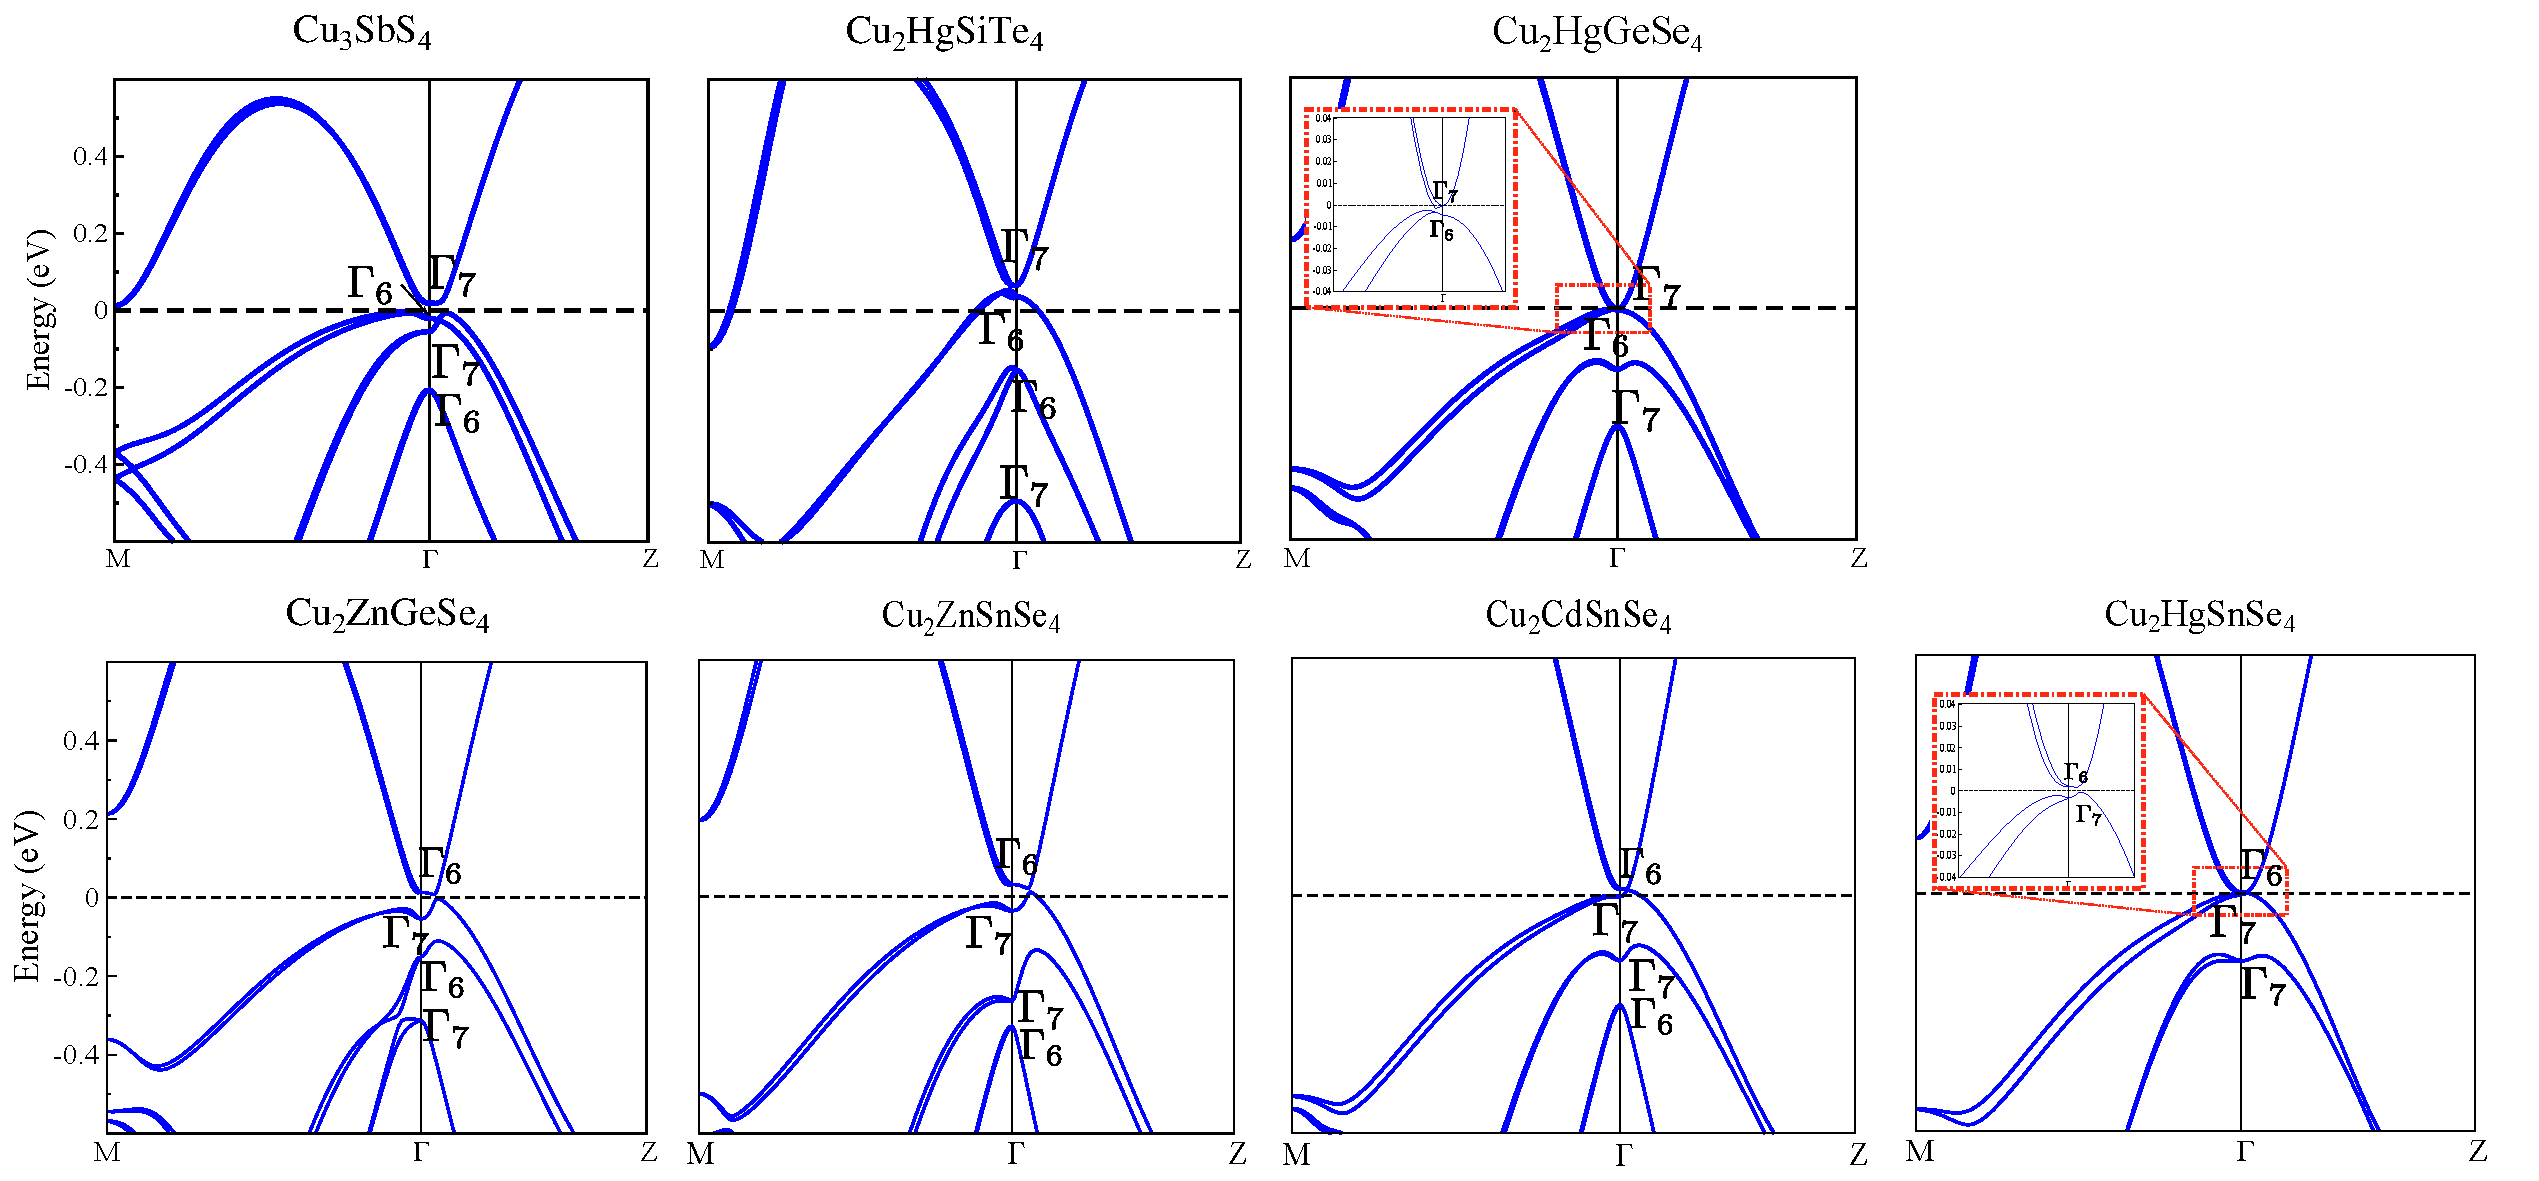
\includegraphics[height=7cm]{s4-figsband.pdf}
\bicaption{
考虑SOC时,这些有$\eta=1$的拓扑材料的能带结构和$\Gamma$点的能带表示。具体地,这些化合物在$k_z=0$面上有非平庸的$\mathbb Z_2$不变量, 但在 $k_z=\frac{\pi}{c}$的面有平庸的$\mathbb Z_2$不变量。~\citep{Qians4}
}
{
The electronic energy bands with SOC and band irreps at the $\Gamma$ point of topological compounds with $\eta=1$. Explicitly, these compounds have a nontrivial $\mathbb Z_2$ invariant in the $k_z=0$ plane, but a trivial $\mathbb Z_2$ invariant in the $k_z=\frac{\pi}{c}$ plane. ~\citep{Qians4}
}
\label{fig:5-s1}
\end{figure*}


\begin{table}[!htb]
    \bicaption{
        考虑SOC时,具有拓扑的化合物的ICSD编号和拓扑分类。~\citep{Qians4}
    }{
     ICSD numbers and topological classifications for these topological compounds with SOC. ~\citep{Qians4}
    }\label{tab:5-s1}
    \centering
    \resizebox{\textwidth}{!}{
    \begin{tabular}{cccc}
    \cline{1-4}
    \cline{1-4}
    \cline{1-4}
    Compound &ICSD Num. &Previous& This work[units: ($\frac{2\pi}{a},\frac{2\pi}{a},\frac{2\pi}{c}$)]\\
    \cline{1-4}
    Cu$_3$SbS$_4$ &  628824\citep{Annamamedov1967}& TI\citep{Wang2010} &TI    \\
    Cu$_2$HgSiTe$_4$ &656152\citep{Haeuseler1991} &TI\citep{tqc2017,Vergniory2019}&TI  \\
     Cu$_2$HgGeSe$_4$ & 627692\citep{Hahn1965}&TI\citep{Wang2010}&TI \\
    Cu$_2$HgGeTe$_4$ & 656155\citep{Haeuseler1991}&TI\citep{tqc2017,Vergniory2019}&TI  \\
    Cu$_3$SbSe$_4$ &  628997\citep{Annamamedov1967}& TI\citep{tqc2017,Vergniory2019}&TI  \\
%    \cline{1-4}
    %Compound &ICSD Num. & Previous& This work [units: ($\frac{2\pi}{a},\frac{2\pi}{a},\frac{2\pi}{c}$)]
    Cu$_2$ZnGeSe$_4$ &627831\citep{Guen1979}&TI\citep{Wang2010}& WSM (0.0036, 0.0, 0.0657)\\
    Cu$_2$ZnSnSe$_4$ &629099\citep{Hahn1965}&TI\citep{Wang2010}& WSM (0.0037, 0.0, 0.0757)\\
    Cu$_2$CdSnSe$_4$ &619784\citep{Hahn1965}& TI\citep{Wang2010}&WSM (0.0014, 0.0,  0.0294)\\
    Cu$_2$HgSnSe$_4$ &627936\citep{Hahn1965}&TI\citep{Wang2010}& WSM (0.0049,  0.0,  0.0238)\\
    Cu$_2$HgSnTe$_4$ &627940\citep{Haeuseler1991}&Trivial\citep{tqc2017,Vergniory2019}& WSM (0.0082,  0.0,  0.0338)\\
    %                         &&  && &Cu$_2$HgSnTe$_4$ &656158\citep{Haeuseler1991}& Trivial\citep{Zhang2018}&WSM (0.0066, 0.0,   0.0191)\\
    \cline{1-4}
    \cline{1-4}
    \cline{1-4}
    \end{tabular}}
    \end{table}
%We find that the band these compounds can he others are qualitatively identical to these two compounds [see more results of other topological candidates in the SM].
%Without loss of generality, we take two examples of \ti~and \wsm~compounds in the main text. The others are qualitatively identical to these two compounds [see more results of other topological candidates in the SM].
我们发现这两种化合物沿着高对称线都有一个带隙。然后,我们计算了$k_z=0$ 和 $k_z=\frac{\pi}{c}$平面上的时间反演不变的$\mathbb Z_2$不变量。 
Wilson loop的计算结果如图~\ref{fig:5-s2}。
%The results of the Wilson loop calculations are presented in Fig.~\ref{fig:5-s2} of Appendix A.
两个$\mathbb Z_2$不变量计算结果为$\nu_{k_z=0}=1$ 和$\nu_{k_z=\frac{\pi}{c}}=0$, 使得$\eta=1$ (或者 $\nu_0=1$ 如果系统在三维布里渊区里完全是开能隙的~\citep{Fu2007topo}) 。这些结果与之前预测的``TIs"的结果是一致的 \citep{Wang2010}。 在本文中,``TIs"代表那些之前预测的121号空间群中$\eta=1$的拓扑材料。

然后,我们进一步检查了电子态的不可约表示~\citep{Gao2020}。在Case I, $\Gamma$点上最低的导带表示是$\Gamma_7$ ,而对于\wsm~最低导带表示是$\Gamma_6$。
$\Gamma_6$ 和 $\Gamma_7$是$\Gamma$点的小群( $D_{2d}$双群)表示的标记。
%%appendix
因为在考虑自旋的体系内 $S_4^4=-1$, $S_4$的本征值为 $\lambda_j=e^{i\pi\frac{2j-1}{4}}$, 其中 $j\in\{0,1,2,3\}$。在具有$S_4$对称性的时间反演不变的体系中,我们提出$S_4$的$z_2$指标的一个一般的定义:
\begin{equation}
  z_2 = \sum_{K\in\{\text{four SIM}\}}\frac{n_K^{2} - n_K^{0}}{2} \quad{\rm mod} \ 2 ,
\end{equation}
这里 $n_K^{i}$ 为在$S_4$不变的动量(SIM)$K$点,有$S_4$ 本征值 $\lambda_i$的占据态能带的数目,细节推导参考文献~\cite{tobedone2019}。
如果这四个SIM也是时间反演不变点(TRIM),那么这个定义与文献~\citep{song2017,haruki2018} 的定义是一致的。

\begin{figure}[!htb]
\centering
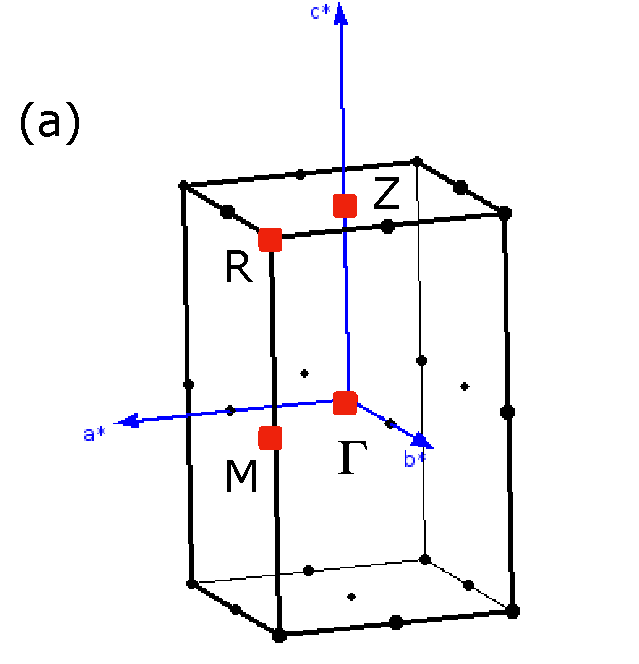
\includegraphics[width=2.5 cm]{s4-scbz.pdf}
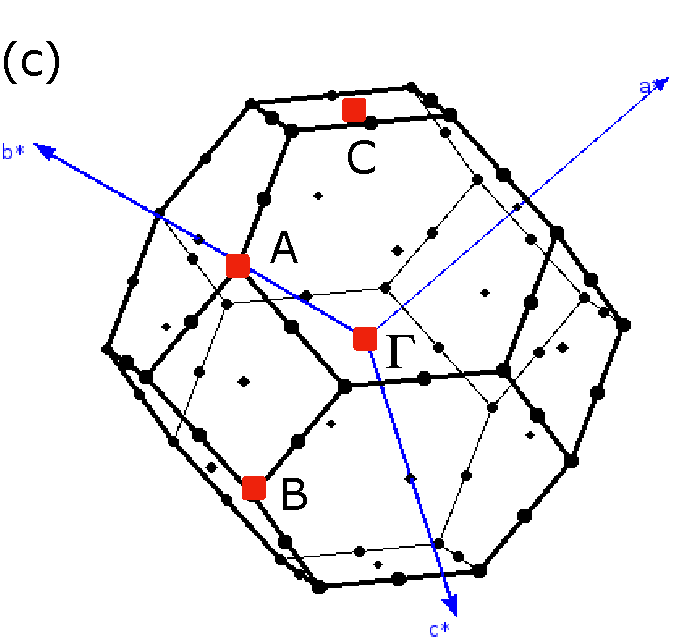
\includegraphics[width=2.5 cm]{s4-fccbz.pdf}
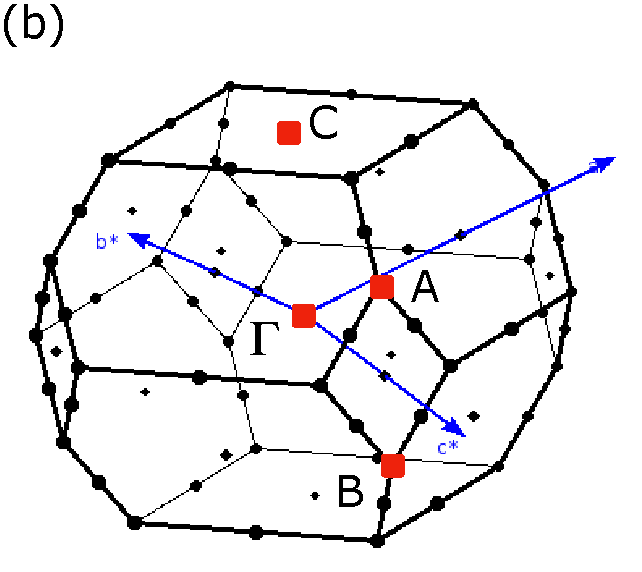
\includegraphics[width=2.5 cm]{s4-bccbz.pdf}
\bicaption{
三维布里渊区和SIM点。我们分别展示了简单晶格(a),面心晶格(b),体心晶格(c)的三维布里渊区。SIM点也在图中标记出来。~\citep{Qians4}
}
{
The 3D BZs and SIM points. We present the 3D BZs for simple lattice (a), and face-centered lattice (b),and body-centered lattice (c)  respectively. The SIM points are labeled too. ~\citep{Qians4}
}
\label{fig:5-bz}
\end{figure}

%\subsubsection*{a. Space group $P{\bar 4}$ (\#81)}
在简单四方结构(SG 81 和它的母群)如图\ref{fig:5-bz} (a) , 四个SIM为$\Gamma[0,0,0]$, $Z[0,0,0.5]$, $M[0.5,0.5,0.0]$, 和 $R[0.5,0.5,0.5]$ (此后,所有$k$点都是以[$\frac{2\pi}{a},\frac{2\pi}{a},\frac{2\pi}{c}$]为单位的笛卡尔坐标)。因为四个SIM也是时间反演不变点,所有点能带都是两重简并的。因此,$n_K^{\frac{1}{2}}~(n_K^{\frac{3}{2}})$ 等于 $n_K^{0}~(n_K^{2})$。
按照文献~\citep{song2017,haruki2018}的定义, $n_K^{\frac{1}{2}}~(n_K^{\frac{3}{2}})$ 是在$K$点满足tr$[D(S_4)]=\sqrt{2}$(tr$[D(S_4)]=-\sqrt{2}$)的Kramers对的数目, 其中$D(S_4)$ 是相应的Kramers对的表示矩阵。
\begin{equation}
  z_2 = \sum_{K\in\{\Gamma,Z,M,R\}}\frac{n_K^{\frac{3}{2}} - n_K^{\frac{1}{2}}}{2} \quad{\rm mod} \ 2 ,
\end{equation}

在面心立方结构(SG 216 和它的母群)如图\ref{fig:5-bz}(b), 四个 SIM是 $\Gamma[0,0,0]$, $C[0,0,1]$, $A[1,0,0.5]$, 和 $B[1,0,-0.5]$。 $A$ 和 $B$ 不是TRIM,没有Kramers简并。因此 $S_4$ $z_2$ 指标定义为,
\begin{equation}
  z_2 = \sum_{K\in\{\Gamma,C,A,B\}}\frac{n_K^{2} - n_K^{0}}{2} \quad{\rm mod} \ 2 ,
\end{equation}

在体心四方结构 (SG 82 和它的母群)如图\ref{fig:5-bz}(c), 四个SIM为$\Gamma[0,0,0]$, $C[0,0,1]$, $A[0.5,0.5,0.5]$, 和 $B[0.5,0.5,-0.5]$。注意到$A$ 和 $B$ 不是TRIM。换句话说,在$A$ 和 $B$点没有Kramers对。所以,$S_4$ $z_2$ 指标的定义为,
\begin{equation}
  z_2 = \sum_{K\in\{\Gamma,C,A,B\}}\frac{n_K^{2} - n_K^{0}}{2} \quad{\rm mod} \ 2 ,
\end{equation}
因为121号群有体心四方结构, 四个SIM的$n_K^{0}$ 和 $n_K^{2}$具体的计算结果在表格~\ref{tab:5-weyls4}给出。
这个$z_{2}$ 指标对于\tii~和\wsm~的计算结果分别为1和0 [参考表格~\ref{tab:5-weyls4}]。

%{\color{blue}NOTE: PLEASE CHANGE ALL S4 $\mathbb Z_2$ to $z_2$.}
\begin{table}[!h]
    \centering
    \caption{
    占据态在SIM点有$S_4$本征值$\lambda_2$和 $\lambda_0$的数目。最后一列展示了计算得到的$S_4$ $z_2$指标。~\citep{Qians4}
      }
      {
    The number of occupied states with $S_4$ eigenvalue $\lambda_2$ and $\lambda_0$ at SIM. The last column shows the determined $S_4$ $z_2$ indicator. ~\citep{Qians4}
      }\label{tab:5-weyls4}
      \begin{tabular}{cccccc}
      \hline
      $n_K^{2},n_K^{0}$ & $\Gamma$ & C & A & B & $S_4~z_2$  \\
      \hline
       \tii~(TI)   & 15,16 & 16,15 & 16,15 & 16,15 & 1 \\
       \wsm~(WSM) & 14,17 & 16,15 & 15,16 & 15,16 & 0 \\
      \hline
      \end{tabular}
\end{table}
    

在三维绝缘相, 强拓扑绝缘体(STI)指标 $\nu_0$~\citep{Fu2007topo} 定义在八个不同的时间反演不变的动量上 [$\Gamma_{i=(n_1n_2n_3)}=(n_1 \bb_1+n_2 \bb_2+n_3\bb_3)/2$, 其中 $n_j=0,1$,$b_j$是倒空间原胞基矢] : 
\begin{equation*}
(-1)^{\nu_0}=\prod_{n_j=0,1}  \delta_{n_1n_2n_3}=(-1)^{\nu_{a_1}}(-1)^{\nu_{a_2}},
\end{equation*}
这里 $\delta_i=\sqrt{det[w(\Gamma_i)]}/Pf[w(\Gamma_i)]$ 其中幺正矩阵 $w_{ij}(\bk)=\braket{u_i(\bk)}{{\cal T}|u_j(\bk)}$。 这里 $\ket{u_j(\bk)}$ 布洛赫函数的周期部分。在 $\bk=\Gamma_i$, $w_{ij} =-w_{ji}$, 所以 Pfaffian $Pf[w(\Gamma_i)]$ 有好的定义。
因为四个$\delta_i$的定义了二维时间反演不变的平面的$\mathbb Z_2$(如果四个$\Gamma_i$形成一个平面),
强拓扑绝缘体对称性指标$\nu_0$也可以通过两个平行平面($a_1$- 面和$a_2$- 面) 的两个不同的$\mathbb Z_2$不变量来定义($\nu_{a_1}$ and $\nu_{a_2}$)来定义, 当$\eta=\nu_0$产生绝缘体。注意,如果三维体态完全开能隙,$\nu_0$可以很好的定义;而只要存在两个完全开能隙的时间反演不变的平面,$\eta$就有好的定义。另一方面,当有额外的$S_4$对称性, 对于绝缘体,$S_4$的$z_2$指标和强拓扑绝缘体的指标$\nu_0$是一致的~\citep{song2017,haruki2018}。
因此,121号空间群的``TIs"中,有平庸的$z_2$指标的\wsm~不是绝缘体。最终,我们发现这些候选材料其实是外尔半金属,有四对外尔点在电荷中性能级。

%%qianyt
因为PBE函数计算得到的能隙一般会被低估,为了检查121号群这些外尔半金属相 (参考表格~\ref{tab:5-s1})能带反转的稳定性,我们使用修正的Becke-Johnson(mBJ)势进行了更精确的计算。由于这些材料能带结构的主要特点是在$\Gamma$点能带的顺序,我们系统的检查了在$\Gamma$点的四条能带(三条价带和一条导带),并将其作为mBJ 参数的($C_\text{mBJ}$) 函数展示在图~\ref{fig:5-mbj}中。对于\tii~的能量顺序为$\Gamma_7$, $\Gamma_6$ 和 $\Gamma_7$ (从高能到低能), 而对于\wsm~是$\Gamma_6$, $\Gamma_7$ 和 $\Gamma_7$ 。随着C$_{\text{mBJ}}$的减小,我们可以清楚的看到表示为 $\Gamma_6$的导带的能量单值减小。相应地,$\Gamma_6$的导带和三条价带相交,两个$\Gamma_6$表示的能带不能相交。在图~\ref{fig:5-mbj}中,C$_{\text{mBJ}}$的临界值用虚线表明,代表$\Gamma_6$的导带与其他更高的价带发生能带反转的地方。
结果表明Cu$_2$HgGeTe$_4$, Cu$_3$SbSe$_4$, Cu$_2$HgSnSe$_4$, 和  Cu$_2$HgSnTe$_4$ 的C$_{\text{mBJ}}$比较大,大概是1.2,所以这些化合物能带反转比较可信。
其中, Cu$_2$HgSnTe$_4$非常有可能是外尔半金属的候选材料,因为能带反转发生在比较大的mBJ参数$C_\text{mBJ}=1.25$。最近的实验\citep{PhysRevB.100.195147}已经通过STM和ARPES中发现Cu$_2$HgSnSe$_4$的半金属的特点。
 


\begin{figure*}[!htbp]
    \centering
    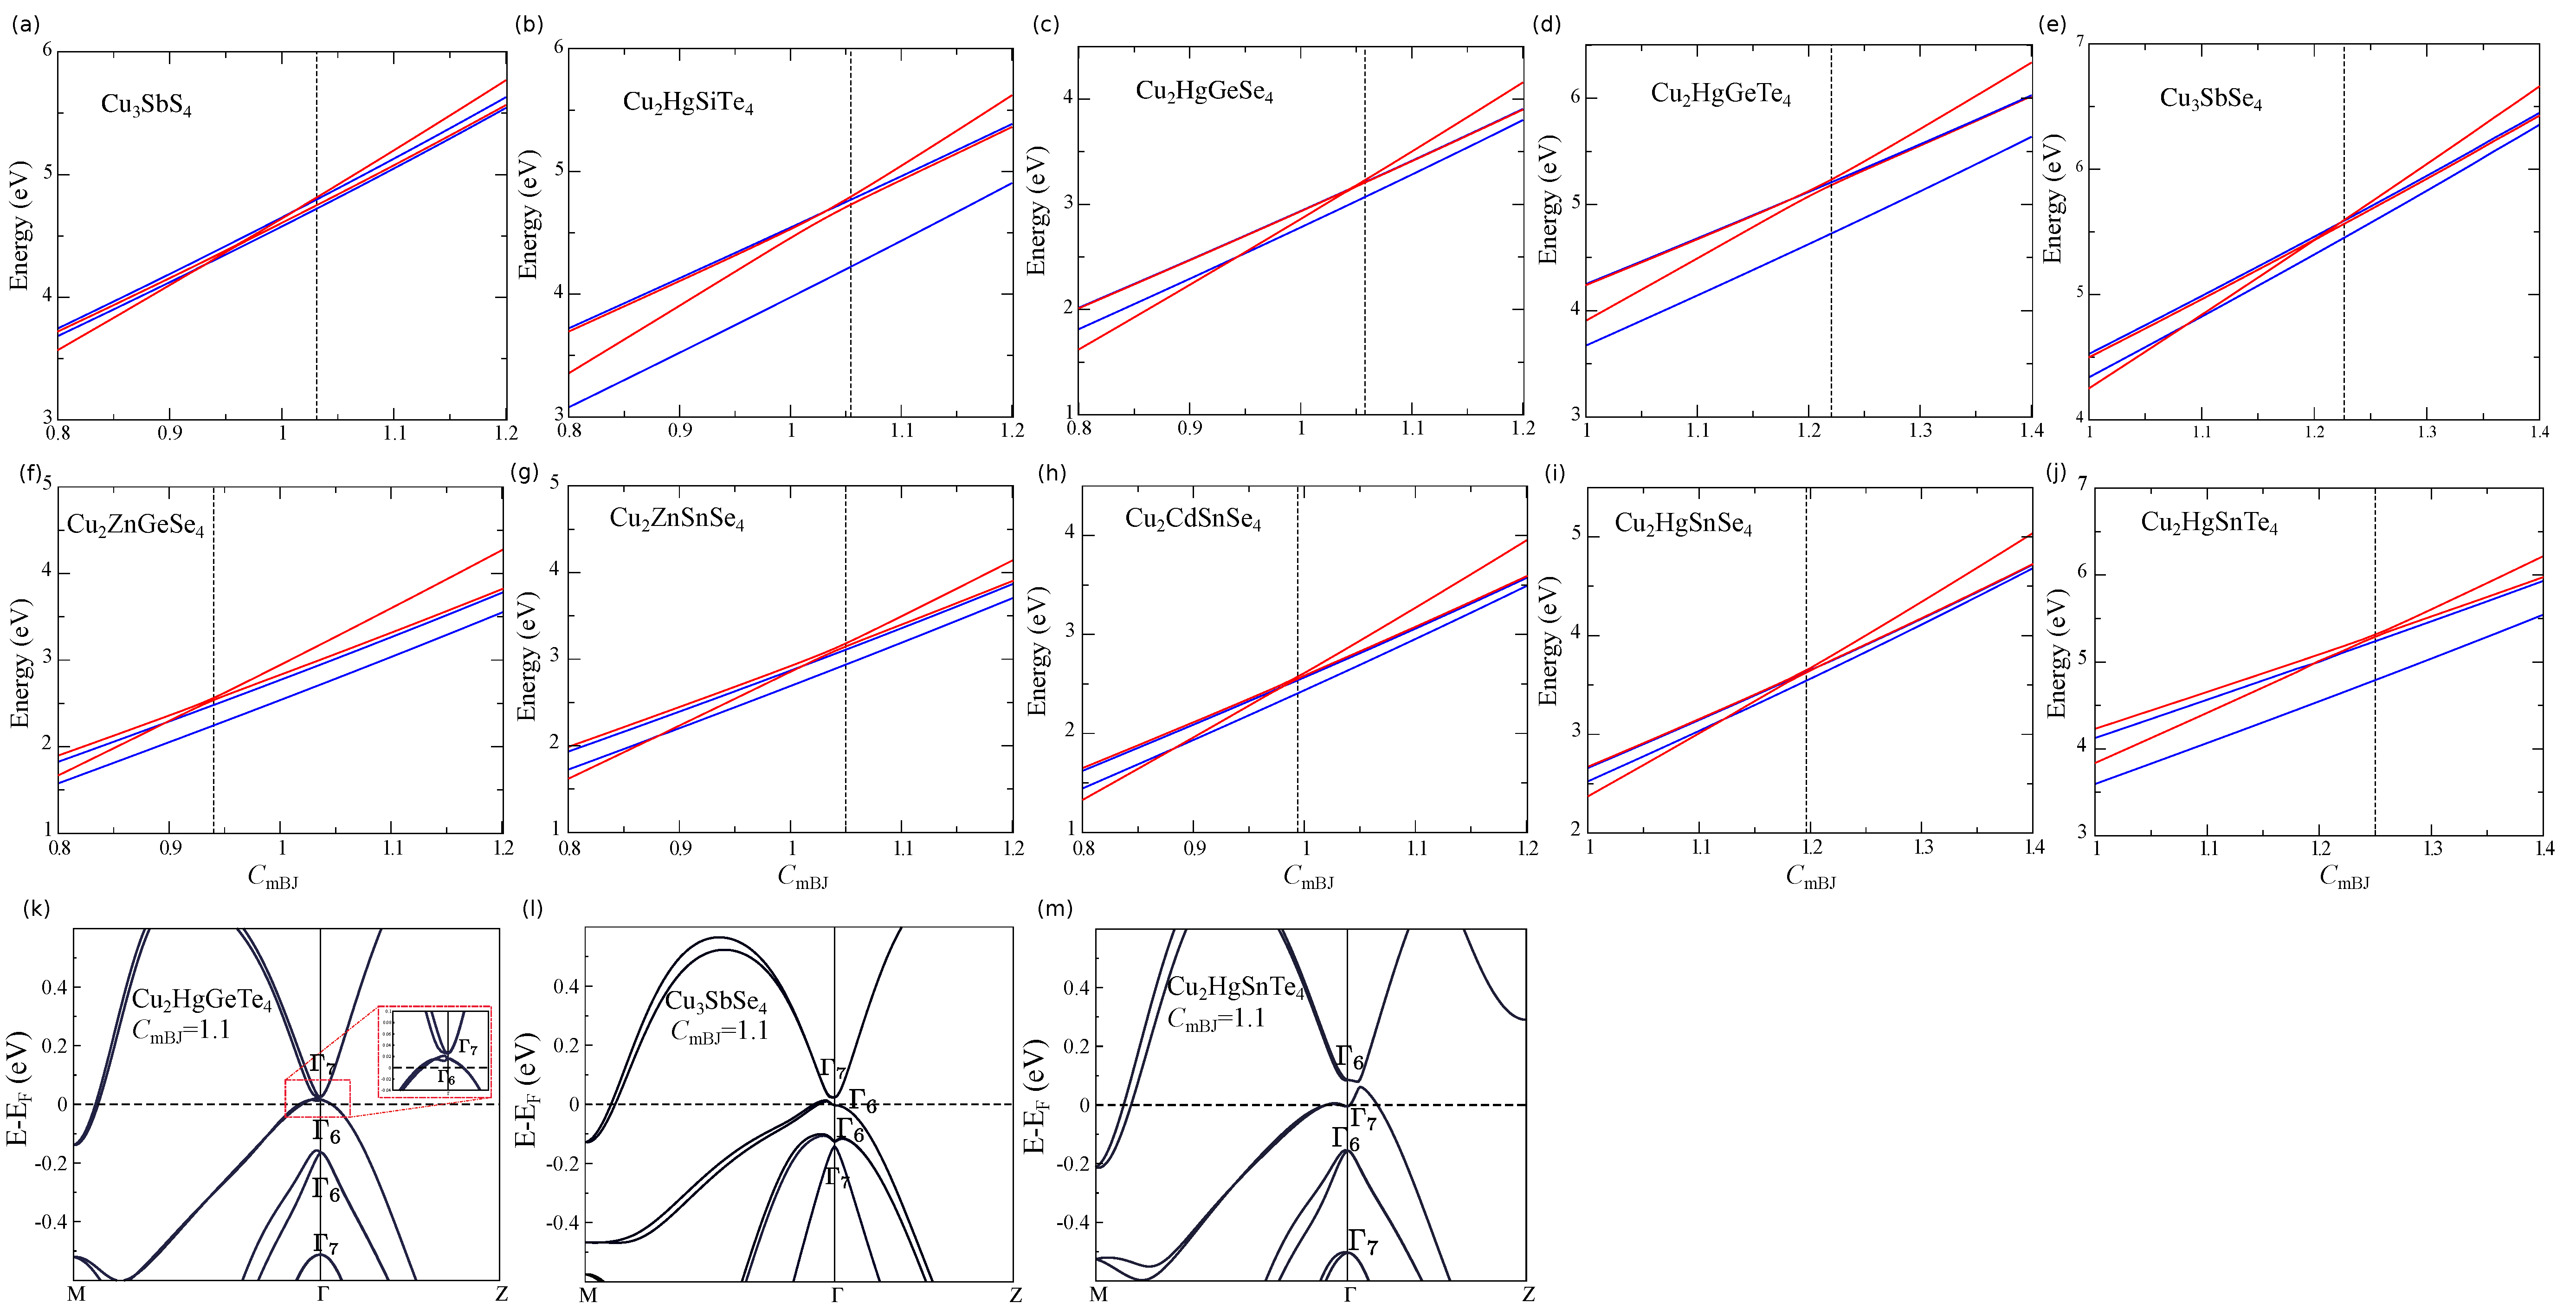
\includegraphics[height=7.5cm]{s4-cmbj.pdf}
    \bicaption{(a-j)展示了不同化合物$\Gamma$处费米能级附近四条能带(三条价带和一条导带)随着$C_\text{mBJ}$ 的演化。表示为$\Gamma_6$和$\Gamma_7$ 的能带分别用红色和蓝色线表示。
    (k-m)代表考虑SOC且$C_\text{mBJ}=1.1$时Cu$_2$HgGeTe$_4$(k), Cu$_3$SbSe$_4$(l), and Cu$_2$HgSnTe$_4$的能带结构。~\citep{Qians4}
    }
    {(a-j) show the band evolutions of four bands near the Fermi level (three valence bands and one conduction band) at the $\Gamma$ point with varying the parameter $C_\text{mBJ}$ for different topological compounds.  The $\Gamma_6$ and $\Gamma_7$ bands are denoted by the red and blue lines, respectively.
    (k-m) present the SOC electronic structures with $C_\text{mBJ}=1.1$ for Cu$_2$HgGeTe$_4$ (k), Cu$_3$SbSe$_4$ (l), and Cu$_2$HgSnTe$_4$ (m), respectively. ~\citep{Qians4}
    }
    \label{fig:5-mbj}
\end{figure*}


\subsection{外尔点和Wilson loop计算}

\begin{figure*}[!htb]
    \centering
    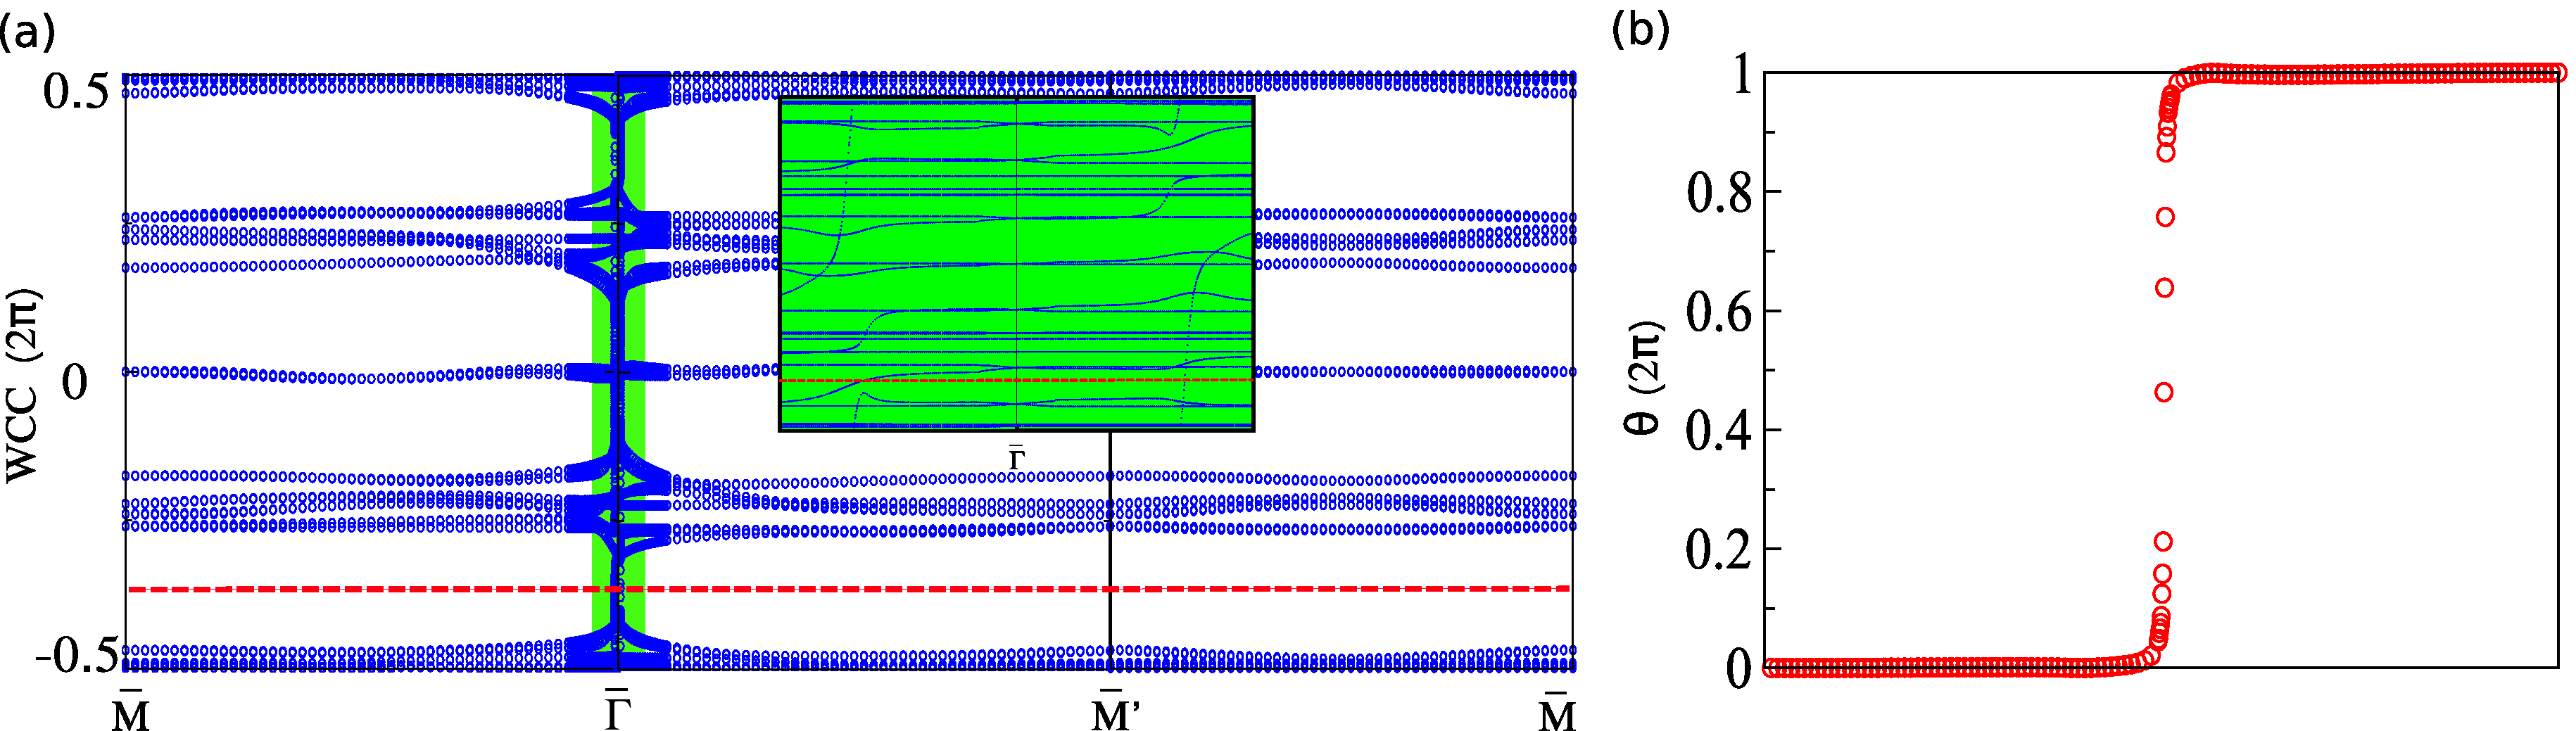
\includegraphics[width=1\textwidth]{s4-fig3.pdf}
    \bicaption{
        (a)\wsmc~沿着路径$\bar M (0.5,0.5)-\bar \Gamma(0,0)-\bar M'(0.5,-0.5)-\bar M(0.5,0.5)$(如图~\ref{fig:5-2})的$k_z$-指向的Wilson loops的WCC。(b) 在包裹外尔点的流形上通过Wilson-loop方法计算的位于[ $0.0036(\frac{2\pi}{a}), 0.0, 0.0657(\frac{2\pi}{c}$) ]的外尔点的手性。~\citep{Qians4}
        }
        {
        (a) The WCC of $k_z$-directed Wilson loops of \wsmc~on the path $\bar M (0.5,0.5)-\bar \Gamma(0,0)-\bar M'(0.5,-0.5)-\bar M(0.5,0.5)$ as marked in Fig.~\ref{fig:5-2}. (b) The chirality of the Weyl point at [$0.0036(\frac{2\pi}{a}), 0.0, 0.0657(\frac{2\pi}{c}$)] calculated by Wilson-loop method on a manifold enclosing it. ~\citep{Qians4}
    } 
    \label{fig:5-3}
    \end{figure*}
%\emph{Weyl points and Wilson loop calculations.} -- 
为了确定外尔点的位置,我们计算了在$k_xk_y$平面,WSM \wsmc~沿着路径: $\bar M [0.5,0.5]-\bar \Gamma[0,0]-\bar M'[0.5,-0.5]-\bar M[0.5,0.5]$(以$[\frac{2\pi}{a},\frac{2\pi}{a}]$为单位 )$k_z$-指向的Wilson loops。如图~\ref{fig:5-3}(a),结果显示有非零的陈数$C=+2$, 这意味着由面内的路径和$k_z$轴构成的二维闭合的流形至少包围有两个手性为+1的外尔点~\citep{Fang92}。
首先, 我们假设在流形的一般位置[$x_1 (\frac{2\pi}{a}),y_1 (\frac{2\pi}{a}),z_1 (\frac{2\pi}{c})$]上有一个手性为+1的外尔点。因为在$k_z=0$面完全打开能隙,$z_1$ 应该是非零的(即,$z_1\neq 0$)。
然后,组合对称性${\cal T}C_{2z}$得出在[$x_1,y_1,-z_1$]位置也有一个同样手性为+1的外尔点。
最后,如果外尔点远离$k_y=0$的面,闭合流形包裹的同样拓扑电荷的外尔点的数目一定是4的倍数,因为两个反幺正对称性:${\cal T}C_{2y}$和${\cal T}C_{2z}$。因此,沿着这条路径相应的陈数是4的倍数。
但是,很明显这不是这个化合物的情况。因此,我们假设外尔点位于$k_y=0$面上:($x_1,0,\pm z_1$)。再仔细检查能隙和在$k_y=0$半平面(即,$k_x>0$)的拓扑电荷后,我们确实发现有两个外尔点位于[$0.0036,0.0,\pm0.0657$]。拓扑电荷可以在包裹外尔点的闭合流形通过Wilson-loop方法计算。位于[$0.0036,0.0,0.0657$]的外尔点的结果如图~\ref{fig:5-3}(b),它的拓扑电荷可以从图中读出为$+1$。考虑到有两个同样手性的外尔点,所以这和图~\ref{fig:5-3}(a)总陈数 ($C=+2$) 的结果是一致的。
%which rules out the existence of other Weyls .


\begin{table*}[!htb]
\bicaption{六带模型对 \tic~(Case I)和 \wsmc~(Case II)的拟合参数。~\citep{Qians4}
}{
The fitting parameters of the six-band model for \tic~(Case I) and \wsmc~(Case II) compounds. ~\citep{Qians4}
}\label{tab:matpara}
\resizebox{\textwidth}{!}{    
\begin{tabular}{ccccccccccccc}
\hline
 Phases  & $A_0$ & $A_1$ & $A_2$ & $B_0$ & $B_1$ & $B_2$ & $C_1$ & $C_2$ & $C_3$ &$\delta_1$ &$\delta_2$ &$\delta_3$ \\
    & (eV) & (eV$\cdot $\AA$^2$) & (eV$\cdot $\AA$^2$) &  (eV) & (eV$\cdot $\AA$^2$) & (eV$\cdot $\AA$^2$) &  (eV$\cdot $\AA$^2$) & (eV$\cdot $\AA$^2$) & (eV$\cdot $\AA) & (eV$\cdot $\AA) &(eV$\cdot$ \AA)&(eV$\cdot $\AA$^3$) \\
\hline
 TI      & -0.055 & 25.121 & 28.679 & -0.001 & -6.642 & -2.872 & 0.244 & 4.691 &  0.325 & 0.020 & 0.013 & 1.103\\
WSM      & -0.151 & 27.895 & 18.702 & -0.020 & -5.451 & -2.369 & 0.300 & 3.300 &  1.137 & -0.034 & 0.108 & 4.400\\
\hline
\end{tabular}}
\end{table*}



\subsection{有效模型和费米弧}
%\emph{Effective model and Fermi arcs.} -- 
为了理解这些材料拓扑非平庸的本质,我们构造了六带有效模型, 包括四条价带 ($\Gamma_6$ 和 $\Gamma_7$) 和两条导带 ($\Gamma_6$)。在顺序为 $\{i|xyz\up\rangle,i|xyz\dw\rangle, |\frac{3}{2}, \frac{3}{2}\rangle, |\frac{3}{2}, \frac{1}{2}\rangle, |\frac{3}{2}, -\frac{1}{2}\rangle, \\|\frac{3}{2}, -\frac{3}{2}\rangle\}$的基矢下, $D_{2d}$-不变的$\bold{k\cdot p}$ 哈密顿量可以写作:
\begin{equation*}
    \begin{split}
        &H(\bk) = \begin{bmatrix}
            M_0& C_3{\mathbb S}^\dagger \\
            C_3{\mathbb S} & H_0+\delta_1 H_A+\delta_2 H_B +\delta_3H_C
        \end{bmatrix}
    \end{split}
\end{equation*}
这里 $M_0=\left(A_0+A_1k_z^2+A_2k_{||}^2\right) {\mathbb I}_{2}$,  $H_0=\left(B_0+B_1k_z^2+B_2k_{||}^2\right){\mathbb I}_{4}+C_1 {\mathbb E}+C_2{\mathbb T}$ ( $\mathbb I_n$是 $n\times n$ 的单位矩阵, $\mathbb E$, $\mathbb T$, $\mathbb S$ 和 $H_C$ 具体形式参考附录~\ref{sec:model}), $H_A= diag\{1,-1,-1,1\}$,
\begin{equation*}
  H_B = \begin{pmatrix}
      0 & -k_+ & 2k_z & -\sqrt{3}k_- \\
      -k_- & 0 & \sqrt{3}k_+ & -2k_z \\
      2k_z & \sqrt{3}k_- & 0 & -k_+ \\
      -\sqrt{3}k_+ & -2k_z & -k_- & 0
  \end{pmatrix}
\end{equation*}
当$A_1=A_2$, $B_1=B_2$, $\delta_1=\delta_2=\delta_3=0$, 这个哈密顿量实际上是 $O_h$-不变的。 $H_A$相是非轴应力,它是的对称性降低到$D_{4h}$。$H_B$相是至关重要的,它会同时破坏$I$ 和 $C_{4z}$, 但是保持$S_{4z}$。
$A_{1,2}>0$ 和 $B_{1,2}<0$ 代表本来是四条价带和两条导带($A_0>B_0$)。
$A_0<B_0$ 代表在$\Gamma$点发生能带反转。最终结果导致,$k_z=0$ 面四条占据态有不平庸的$\mathbb Z_2$不变量(即 $\nu_{k_z=0}=1$)。 % while $\nu_{k_z=\pi}=0$).
如果$\delta_1>0$, 是没有无能隙点的拓扑绝缘体。如果$\delta_1<0$, 是有四对外尔点的外尔半金属。
~\tic~和~\wsmc~的拟合参数在表格~\ref{tab:matpara}中给出,而且相应的能带结构在图~\ref{fig:5-s3}中展示。
\begin{figure}[!htb]
    \centering
    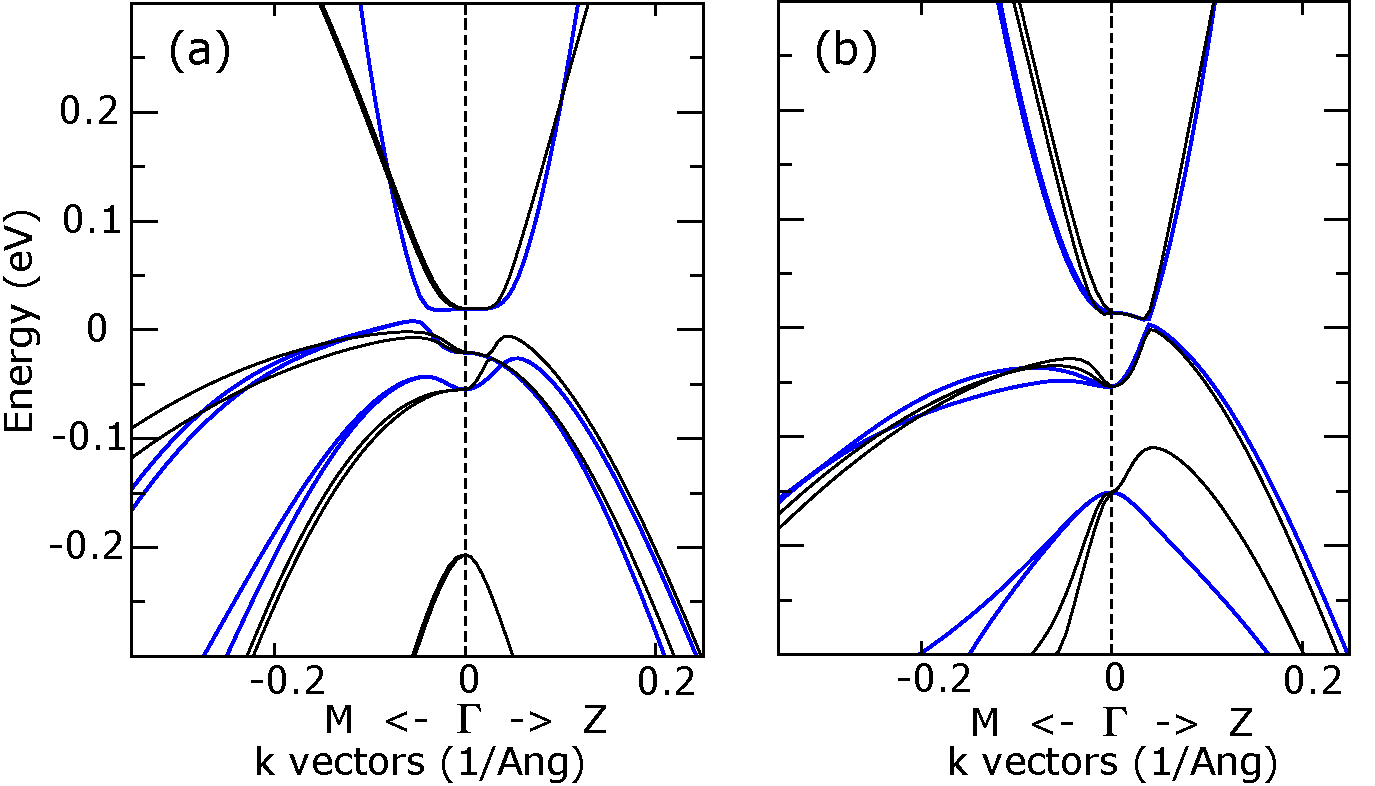
\includegraphics[height=4.3 cm]{s4-figs3.pdf}
    \bicaption{
        ~\tic~(a)和 \wsmc~(b)在$\Gamma$点附近的拟合的能带结构,拟合参数列在表格5.3中。其中黑色的线是有第一性原理计算得到的能带结构,蓝色的线是由六带模型拟合的结果。~\citep{Qians4}
    }
    {
    The fitted electronic energy bands around the $\Gamma$ point of ~\tic~(a) and ~\wsmc~(b) with fitting parameters shown in Table 5.3, where the black lines are the band structures from first-principles calculations and the blue lines are the results of the fitted effective six-band model. ~\citep{Qians4}
    }
    \label{fig:5-s3}
\end{figure}

%{\color{red}Note that the six-band model is the minimal model to describe band inversion and topological phase transation process in these candidates at $\Gamma$ point.  The $k\cdot p$ Hamiltonian was blockly built by using the invariant method. Firstly, we build the six band Luttinger model describing the $\Gamma^-_7$ and $\Gamma_8^+$ bands which label the O$_h$ group. Then by introducting the band inversion and strain term, we can reproduce the process of Weyl fermion's emergence.  Proper parameters are chosen to satisfy the condition of Weyl fermions mentioned above. }

为了获得外尔半金属相\wsm~的费米弧表面态~\citep{Wan2011,xu2011chern},我们通过引入变换: $k_{i}\rightarrow \frac{1}{L_{i}}\text{sin}[k_{i}L_{i}]$ 和 $k_{i}^2\rightarrow\frac{2}{L_{i}^2}(1-\text{cos}[k_{i}L_{i}])$,其中 $i=x,y,z$~\citep{wang2013three},将六带模型转化为四方晶格的紧束缚模型。
%k_{i}\rightarrow sin[k_{i}L_{i}], 
%k_{i}^2\rightarrow\frac{2}{L_{i}^2}(1-cos[k_{i}L_{i}]) (L_{x,y}=a,L_{z}=c).
我们使用迭代方法去获得半无限大体系的表面格林函数~\citep{WU2017,Sancho_1985}。表面格林函数的虚部是表面上的局域表面态 (LDOS) 。在半无限大(001) 和 (100) 表面计算得到的LDOS展示在图~\ref{fig:5-4}。因为外尔点恰好在电中心能级, 我们仅看到连接外尔点的费米弧态。在(001) 表面,两个同样手性的外尔点投影到同一个位置,所以每个投影点有两个弧。在 (100) 表面,投影的拓扑电荷展示在图~\ref{fig:5-4} (b) , 两个弧穿过$k_z=0$ 的线,因为它是有不平庸的$\mathbb Z_2$不变量的$k_z=0$面的边界。
\begin{figure}[!hb]
\centering
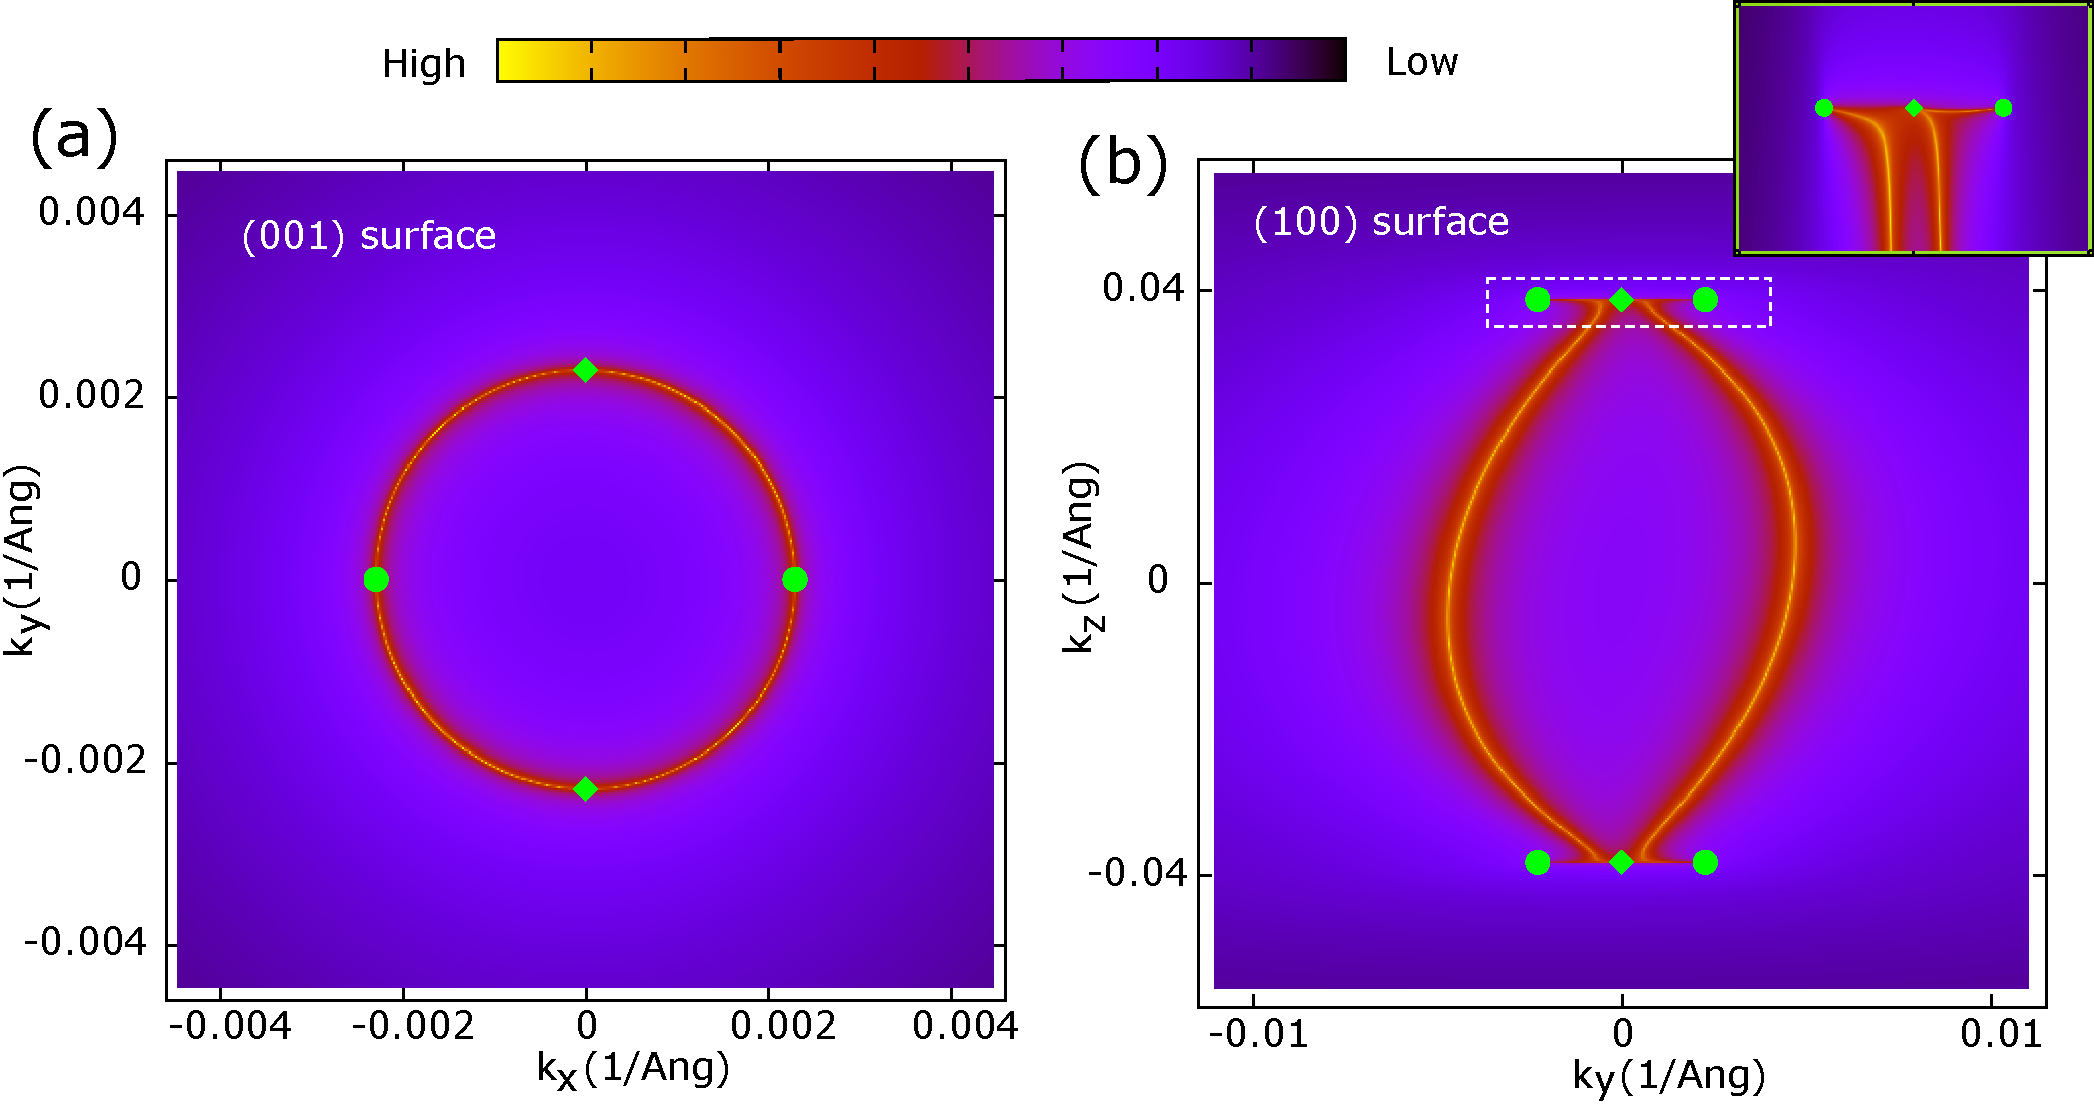
\includegraphics[width=7.5 cm]{s4-fig4.pdf}
\bicaption{
六带模型的表面费米弧。(a)(001)表面BZ的表面费米弧。(b)(100)表面BZ的表面费米弧。不同的手性的投影的外尔点用方块或者圆形表示。~\citep{Qians4}
}
{
Surface Fermi arcs of six-band model. (a) Surface Fermi arcs in the (001) surface BZ. (b) Surface Fermi arcs in the (100) surface BZ. The projected Weyl points are shown as square and circle points for different chiralities. ~\citep{Qians4}
}
\label{fig:5-4}
\end{figure}


\section{结论}
%\emph{Discussion.} --


对于外尔半金属的判据$\eta\neq z_2$可以广泛应用于其他具有$S_4$对称性的空间群。例如,我们计算了122号群的WSM CuTlSe$_2$的$z_2$不变量和$\eta$~\citep{Haijun2016}, 这个材料之前也被认为是拓扑绝缘体~\citep{Feng2011}。$\eta=1$ 和 $z_2=0$的结果表明这是个外尔半金属。另外,这个判据也可以用来理解应变的HgTe类材料的外尔相(压缩应变)和拓扑绝缘体相(拉伸应变)~\citep{HgTenc2016}。

总结一下,基于DFT计算,我们证明了先前在没有中心反演对称性但保持$S_{4z} $对称性的空间群121中预测的``TI'',实际上可以分为两种情况:$z_2=1 $ (\tii) 和$z_2=0$ (\wsm)。
这些``TIs"共同特点是时间反演的$\mathbb Z_2$不变量在$k_z=0$ 和 $k_z=\frac{\pi}{c}$的面分别为1 和 0,导致$\eta=1$。
这和绝缘相里\tii~的$S_4~z_2=1$的结论是一致的。
但是,对于``TIs"中有$S_4~z_2=0$的\wsm~实际上是外尔半金属, 这是之前没有发现的。
他们也可以作为有平庸的对称指标的拓扑材料的典例~\citep{song2017,wangprl2019}。
在 $k_{x,y}=0$面上发现四对外尔点,每个平面上四个外尔点手性相同。
我们的工作纠正了之前对这些材料已有的认识,并且预测了更多的外尔半金属候选材料,这些材料可以在之后的实验中进一步检验。
更重要的是,在时间反演不变体系中使用对称性指标和拓扑不变量方法 (即 $\eta\neq z_2$) 对于搜索外尔半金属提供了新的途径。
在此工作后期,我们对数据库中所有具有S$_4$但不具有中心反演的体系进行了高通量计算~\citep{tobedone2019},发现很多有趣外尔半金属材料。为实验和理论的研究提供了很多可选择的平台。相信我们的工作在未来将有助于大量预测外尔半金属。
\ \\


% %\newpage
% \begin{figure}[!htb]
% \centering
% 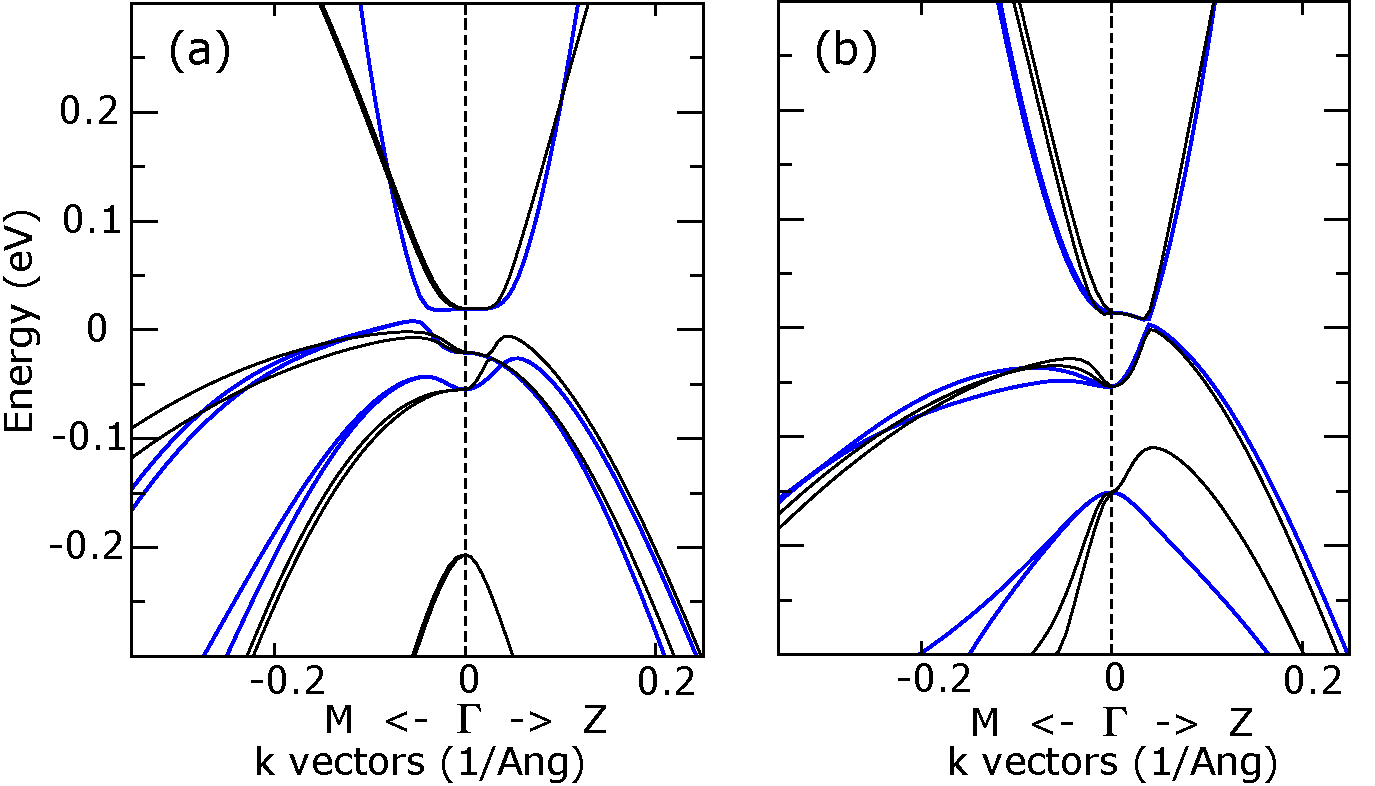
\includegraphics[height=5 cm]{s4-figs3.pdf}
% \caption{(Color online)
% The fitted electronic energy bands around the $\Gamma$ point of ~\tic~(a) and ~\wsmc~(b) with fitting parameters shown in Table I, where the black lines are the band structures from first-principles calculations and the blue lines are the results of the fitted effective six-band model.
% }
% \label{fig:5-s3}
% \end{figure}


\chapter{总结与展望}\label{chap:summary}
本论文主要介绍了我在博士期间的四个研究工作。我的工作主要是基于拓扑能带理论,利用第一性原理,结合Wannier紧束缚模型和$\mathbf{k\cdot p}$模型,研究材料的拓扑性质。我的工作可以分为两个方面:一方面是新的拓扑材料的计算和预言,另一方面是利用现有的理论知识,对已知拓扑体系的物性进行理论解释,进一步发展新的方法,为寻找新的拓扑材料提供理论依据。

在拓扑材料预言方面,我们预言了在超导体HfRuP家族具有拓扑非平庸的电子结构,其中HfRuP属于第二类外尔半金属,而ZrRuAs,ZrRuP和HfRuAs属于拓扑晶体绝缘体。我们与石友国老师团队合作,成功生长了HfRuP和ZrRuAs单晶样品,以这两个材料为代表,研究了其电阻和磁化率随温度变化的规律,发现两个材料都在超导转变温度后有零电阻和迈斯纳效应,成功证明了HfRuP家族的超导性。与此同时,我们与钱天老师和丁洪老师的团队合作,研究了这两个的角分辨光电子能谱,发现与理论计算吻合的非常好。我们预言这个家族的拓扑性质和本征的超导性质相结合极有可能实现拓扑超导,其中HfRuP可能通过外尔半金属相和超导性结合实现拓扑超导,ZrRuAs、ZrRuP或HfRuAs可能通过拓扑晶体绝缘体相和超导性结合实现镜面拓扑超导。

关于LaSbTe的研究和S$_4$外尔半金属的研究构成本论文的第二个方面,这些工作的意义主要体现在进一步深入理解材料拓扑物性,为寻找新的拓扑材料提供理论依据。首先总结一下关于LaSbTe的研究。我们知道所有的晶体点群对称性保护的拓扑态都可以通过堆叠低维的拓扑态来实现。利用实空间构造的方法,方辰老师团队完成了所有磁群从对称性指标到拓扑不变量的映射关系,在拓扑分类方面取得了非常重要的成果。但是这个方法的不足之处是物理图像并不清晰,具体来讲就是在实际材料中,即使知道层构造的方式,但很难理解实空间相应的密勒面可以看作是低维的拓扑态。我们利用层状材料LaSbTe,可以完美的解释这一物理图像。我们发现,这个材料有两个拓扑相,一个是四方的弱拓扑绝缘体相\ti,一个是正交的拓扑晶体绝缘体相\tci~。通过声子谱计算分析,我们知道每一个正交相结构的原胞都可以看作是两个四方相结构的发生结构相变之后沿着$c$轴方向堆叠得到的。利用层构造方法分析后,我们发现四方相\ti~每一层都可以看作是一个二维拓扑绝缘体。正交相\tci~恰好可以看作是位于密勒面(001;$\frac{1}{4}$)和(001;$\frac{3}{4}$)位置的两个\ti~发生形变后沿着c方向的堆叠得到。并且通过这种层构造的方式,可以很容易推导得到的相应的对称性指标和拓扑不变量。拓扑不变量告诉我们这个拓扑晶体拓扑绝缘体\tci~具有沙漏型表面态和($d-2$)维的棱态。我们使用第一性原理结合Wannier函数,Wilson-loop谱的方法,验证了该体系确实存在上述性质。这是第一次找到一个实验可以得到的材料能够生动形象地将实空间的层构造和动量空间的能带拓扑相对应。相信这个例子为我们理解拓扑晶体绝缘体和拓扑绝缘体的关系和物理本质提供了非常好的平台,由此也可以思考通过层构造的方法,设计新的拓扑材料。

由于外尔半金属除了平移对称性之外,不受任何晶体对称性的保护,所以判断外尔半金属没有相应的对称性指标。但是我们发现有一类具有旋转对称性C$_4$和空间反演对称性$I$的组合对称性S$_4$的体系,我们可以通过定义的S$_4$的对称性指标$\eta$和时间反演对称性指标$z_2$的不匹配,即$\eta \neq z_2$来判断体系存在外尔点。并且通过仔细研究一系列锡矿结构的铜基硫族元素化物,发现之前被认为是拓扑绝缘体的一些材料满足$\eta \neq z_2$,因而是外尔半金属。通过Wilson-loop计算陈数,确实证实了在这些材料中存在外尔点,验证了我们的理论。后来,我们还进一步对所有的具有S$_4$对称性的体系进行了系统的研究,定义统一的S$_4$不变量,由此对材料数据库进行了高通量的计算,发现了很多新奇的外尔半金属~\citep{tobedone2019}。相信我们的理论可以在今后的科研中对于理解量子材料的拓扑物性,预言新的拓扑材料方面起到重要的作用~\citep{gapless2020}。

%-
%-> Appendix
%-
\cleardoublepage%
\appendix% initialize the environment
\chapter{{S$_4$}外尔半金属的六带模型推导}\label{sec:model}
在此附录里将推导满足S$_4$对称性的外尔半金属的六带模型。首先从$O_h$对称性出发,再加上$z$方向的非轴应力得到满足$D_{4h}$对称性的哈密顿量。再进一步破坏时间反演对称性$I$和$C_{4z}$,但保持S$_{4z}$对称性,最终获得$D_{2d}$不变的六带有效模型。推导过程如下:

%\section{$S_4$外尔半金属的六带模型推导}\label{sec:model}
\begin{table*}[!htb]
    \setlength{\tabcolsep}{0.5mm}{
    \caption{在$\Gamma_7^-$和$\Gamma_8^+$表示的基矢下,$O_h$小群生成元(即 $C_{3,111}$ 和 $C_{4z}$)的矩阵表示。~\citep{Qians4}}
    {The matrix representations of the generators (\ie $C_{3,111}$ and $C_{4z}$) of $O_h$, given under the basis of $\Gamma_7^-$ and $\Gamma_8^+$, respectively.~\citep{Qians4}
    }\label{tab:rep}
    \begin{tabular}{ccc}
    \hline
    &     $\Gamma_7^-$   &   $\Gamma_8^+$ \\
    \hline
     C$_{3,111}$  &     $\frac{1}{2}\left(\begin{array}{cc} 1-i & -1-i \\ 1-i & 1+i \end{array}\right)$   &   $\frac{1}{4}\left(\begin{array}{cccc} -1-i & -\sqrt{3}+\sqrt{3}i & \sqrt{3}+\sqrt{3}i & 1-i \\ -\sqrt{3}-\sqrt{3}i & -1+i & -1-i & -\sqrt{3}+\sqrt{3}i \\ -\sqrt{3}-\sqrt{3}i & 1-i & -1-i & \sqrt{3}-\sqrt{3}i \\ -1-i & \sqrt{3}-\sqrt{3}i & \sqrt{3}+\sqrt{3}i & -1+i \end{array}\right)$ \\
%    \hline
     C$_{4z}$     &    $-\frac{\sqrt{2}}{2}\left(\begin{array}{cc} 1-i & 0 \\ 0 & 1+i \end{array}\right)$   &   $\left(\begin{array}{cccc} -(-1)^{\frac{1}{4}} & 0 & 0 & 0 \\ 0 & -(-1)^{\frac{3}{4}} & 0 & 0 \\ 0 & 0 & (-1)^{\frac{1}{4}} & 0 \\ 0 & 0 & 0 & (-1)^{\frac{3}{4}} \end{array}\right)$ \\
%    \hline
     $I$ & $-{\mathbb I_2}$&  ${\mathbb I_4}$\\
%    \hline
     $\cal{T}$     &    $-\left(\begin{array}{cc} 0 & -1 \\ 1 & 0 \end{array}\right)K $ & $ \left(\begin{array}{cccc}0 & 0 & 0 & 1 \\ 0 & 0 & -1 & 0 \\ 0 & 1 & 0 & 0 \\ -1 & 0 & 0 & 0\end{array}\right)K $ \\
    \hline
    \end{tabular}
    }
\end{table*}
%%%

在$O_h$对称性下,使用$\Gamma_7^-$和 $\Gamma_8^+$能带,可以构造一个六带的有效模型。具体地,在基矢$\{i|xyz\uparrow\rangle, i|xyz\downarrow\rangle, |\frac{3}{2}, \frac{3}{2}\rangle, |\frac{3}{2}, \frac{1}{2}\rangle, |\frac{3}{2}, -\frac{1}{2}\rangle, |\frac{3}{2}, -\frac{3}{2}\rangle\}$下, $O_h$-不变的 $\bold{k\cdot p}$ 哈密顿量可以写作:
%
%
%\begin{widetext} 
\begin{equation}
    \begin{split}
        H'= \begin{bmatrix}
            \left(A_0+A_2k^2\right) {\mathbb I}_{2}& C_3{\mathbb S}^\dagger \\
            C_3{\mathbb S} & H_0
        \end{bmatrix}\\
\end{split}
\end{equation}
%      \text{ with}~H_0=(B_0+B_2k^2){\mathbb I}_{4}+C_1 {\mathbb E}+C_2{\mathbb T}, 
% \text{where}  &~  k\equiv k_x^2+k_y^2+k_z^2 \text{~and ${\mathbb I}_n$ is an $n$-dimensional identity matrix,} 
这里~$H_0=(B_0+B_2k^2){\mathbb I}_{4}+C_1 {\mathbb E}+C_2{\mathbb T}$, 其中~ $k\equiv k_x^2+k_y^2+k_z^2 \text{~和 ${\mathbb I}_n$ 是一个 $n$-维单位矩阵}$,

%\begin{tiny}
\begin{equation}
    \begin{split}
        {\mathbb E} = \begin{pmatrix}
            2k_z^2-k_x^2-k_y^2 & 0 & \sqrt{3}(k_x^2-k_y^2) & 0 \\
            0 & -(2k_z^2-k_x^2-k_y^2) & 0 & \sqrt{3}(k_x^2-k_y^2) \\
            \sqrt{3}(k_x^2-k_y^2) & 0 & -(2k_z^2-k_x^2-k_y^2) & 0 \\
            0 & \sqrt{3}(k_x^2-k_y^2) & 0 & 2k_z^2-k_x^2-k_y^2
        \end{pmatrix}
            \end{split}
\end{equation}
%\end{tiny}
\begin{equation}
    \begin{split}
& {\mathbb T} = \begin{pmatrix}
            0 & k_- k_z & -ik_x k_y & 0 \\
            k_+ k_z & 0 & 0 & -ik_x k_y \\
            ik_x k_y & 0 & 0 & -k_- k_z \\
            0 & i k_x k_y & -k_+ k_z & 0
        \end{pmatrix}~\\
    \end{split}
\end{equation}
\begin{equation}
    \begin{split}
&    {\mathbb S} = \begin{pmatrix}
        k_+ & 2k_z \\
        0 & -\sqrt{3}k_+ \\
        \sqrt{3}k_- & 0 \\
        2k_z & -k_-
    \end{pmatrix}
    \end{split}
\end{equation}


其中$O_h$群生成元的矩阵表示如表格~\ref{tab:rep}。


为了获得$D_{4h}$对称性, 我们可以简单地改变$A_2k^2~(B_2k^2)$ 到 $A_1k_z^2+A_2k_{||}^2~(B_1k_z^2+B_2k_{||}^2)$ ,而且加上一个对角项$H_A$到 $H_0$中, $H_A$是个在$z$方向的非轴的应力。简单地可以取 $H_A$为$Diag\{1,-1,-1,1\}$。
然后,为了破坏中心反演对称性$I$和$C_{4z}$但是保持S$_{4z}$, 加入了$H_B$ ($\bk$的一阶项) 和 $H_C$ ($\bk$的一阶项)。$D_{2d}$-不变的哈密顿量可以推导得到:


\begin{equation*}
    \begin{split}
        &H(\bk) = \begin{bmatrix}
            M_0& C_3{\mathbb S}^\dagger \\
            C_3{\mathbb S} & H_0+\delta_1 H_A+\delta_2 H_B +\delta_3H_C
        \end{bmatrix}
    \end{split}
\end{equation*}
其中 $M_0=\left(A_0+A_1k_z^2+A_2k_{||}^2\right) {\mathbb I}_{2}$ 和 $H_0=\left(B_0+B_1k_z^2+B_2k_{||}^2\right){\mathbb I}_{4}+C_1 {\mathbb E}+C_2{\mathbb T}$ ,额外的一阶项$H_B$为,
\begin{equation}
  H_B = \begin{pmatrix}
      0 & -k_+ & 2k_z & -\sqrt{3}k_- \\
      -k_- & 0 & \sqrt{3}k_+ & -2k_z \\
      2k_z & \sqrt{3}k_- & 0 & -k_+ \\
      -\sqrt{3}k_+ & -2k_z & -k_- & 0
  \end{pmatrix}
\end{equation}
三阶项 $H_C$为,
\begin{equation}
    H_{C}= k_z(k_x^2-k_y^2)J_z+ k_x(k_y^2-k_z^2)J_x+ k_y(k_z^2-k_x^2)J_y
\end{equation}
其中,
\begin{equation}
\begin{split}
&    J_x=\begin{pmatrix}
       0 & \sqrt{3} & 0 & 0\\
       \sqrt{3} & 0 & 2 & 0\\
       0 & 2 & 0 & \sqrt{3}\\
       0 & 0 & \sqrt{3} & 0
    \end{pmatrix};~\\
 &   J_y=\begin{pmatrix}
       0 & -\sqrt{3}i & 0 & 0\\
       \sqrt{3}i & 0 & -2i & 0\\
       0 & 2i & 0 & -\sqrt{3}i\\
       0 & 0 & \sqrt{3}i & 0
    \end{pmatrix};~\\
&    J_z=\begin{pmatrix}
       3 & 0 & 0 & 0\\
       0 & 1 & 0 & 0\\
       0 & 0 &-1 & 0\\
       0 & 0 & 0 &-3
    \end{pmatrix};~
    \end{split}
\end{equation}
%
参数已经在正文中给出,模型的拟合的能带结构如图~\ref{fig:5-s3}.


%\clearpage
%\section{对称性联系的{$\mathbf{k}$}点的交叠矩阵和投影矩阵}
%???





% appendix content
%-
%-> Backmatter: bibliography, glossary, index
%-
\backmatter% initialize the environment
\intotoc*{\cleardoublepage}{\bibname}% add link to toc
\artxifstreq{\artxbib}{bibtex}{% enable bibtex
    \bibliography{Biblio/ref}% bibliography
}{%
    \printbibliography% bibliography
}
%---------------------------------------------------------------------------%
%->> Backmatter
%---------------------------------------------------------------------------%
\chapter[致谢]{致\quad 谢}\chaptermark{致\quad 谢}% syntax: \chapter[目录]{标题}\chaptermark{页眉}
\thispagestyle{noheaderstyle}% 如果需要移除当前页的页眉
%\pagestyle{noheaderstyle}% 如果需要移除整章的页眉

在论文接近尾声的时候,仿佛看到了我的博士生活也接近尾声了。
在物理所生活的五年,是我学生生涯的最后阶段,也是我收获最丰富的五年。这里有太多太多的美好值得回忆,我希望在这里向每一位曾经帮助过我的人说一声谢谢。

首先要感谢的就是我的导师翁红明老师。翁老师不仅是我科研工作的领路人,也在我科研生活的方方面面影响着我。%第一次来北京找翁老师的画面仍然历历在目:翁老师先是询问了我的科研兴趣,然后认真地向我介绍了课题组的情况,并仔细的告诉我如何在网上找到老师的文献,最后还送给我两本杂志,并嘱咐我认真阅读文献。
刚进组时,每次和老师讨论,或是在电梯里碰面,翁老师都不厌其烦地告诉我一定要多读文献。虽然我的基础不好,但是翁老师总是会循循善诱地给我讲解一些很基础的问题,严格要求我对每一个细节都要掌握清楚,不能模棱两可,指导我一步步从对科研一无所知到可以独当一面。翁老师还经常指导我和一些实验组合作,在这个过程中,我发现翁老师不光有丰富的理论知识,对实验的细节也驾轻就熟。老师告诉我这些知识就是要靠不断的积累、学习。
在这些合作中,我不仅向实验组的老师和同学们学到很多知识,也让我意识到不光要会计算,还要能理解实验的可行性,这对于我今后寻找有价值的课题非常重要。在组里的这几年,翁老师还为我提供了很多学习的机会,包括组里举办的一些workshop,其他单位组织的关于拓扑理论和第一性原理相关的会议。每次会议我都能学习到很多知识,还能有机会见识自己所在的领域里的各位前辈们的科研品味、态度和精神,有时还有机会能结交到一些很优秀的同龄人,这些都是我今后科研道路上的宝贵财富。

我还要感谢‪Oleg Yazyev‬老师和吴泉生师兄、张胜男师姐对我科研工作和生活初期的耐心指导。Oleg老师是一个非常耐心的老师,经常对当时几乎什么都不懂的我给予鼓励。他看待问题总是可以做到一针见血,每次组会上,当我刚刚把自己遇到的困难说出来,他就能立马抓住问题的本质,告诉我可以在哪些方面寻求突破。吴师兄能力非常强,不仅有扎实的理论功底上,超强的编程能力,还有非常强的学习能力,独特的科研品味。我在第一性原理计算方面的相关知识几乎是吴师兄手把手教的,师兄总是很有耐心的一边指导我,一边鼓励我,还“骗”我他读研时也像我一样什么都不懂。在师兄的“欺骗”下,我一直自我感觉良好,虽然遇到一些困难,但也能够乐观面对,这使得我在后知后觉中一步步走上科研的正轨。张胜男师姐在生活方面给了我非常非常多的帮助,在科研上我遇到困难时也经常鼓励我,在此表示真心的感谢。

我还想感谢方辰老师。和方老师的合作并不多,但是方辰却一直是我的精神偶像。听过方老师的很多报告,也拜读过方老师的很多工作,可以说我在拓扑理论方面的大部分知识是从方老师的工作中学习到的。我的LaSbTe这个工作也是完全依赖于方辰老师层构造的方法。那一次方老师一遍遍认真地帮我修改论文,还告诫我论文里一定不能有低级错误。后来又有幸经常参加方老师组内聚会,聆听老师对科研的认识和见解。在我博后申请方面,方老师也帮了我很大的忙,不仅帮我写推荐信,还认真地教我如何正确使用一些语法。这次的三月会议,也有幸聆听了方老师对我讲解的工作提供的指导意见。唯一遗憾的是我一直因为比较怂,有问题却不敢向方老师请教,总怕被老师嫌弃而丧失了很多次和老师学习的机会。虽然在紧张的科研工作和生活中与方老师的交集不多,但深深被方老师的为人所折服。希望今后也能像方老师一样在科研和生活两方面做好自己。

我还想感谢王志俊师兄对我科研工作的指导。王师兄工作非常努力,认真。师兄在科研工作中事无巨细,让我学到了很多。师兄的想法很多,给了我很多材料去探索,我能够顺利毕业也离不开王师兄的指导。

我还想感谢每一位合作者,感谢方忠老师,物理所石友国老师,周兴江老师,刘国东老师,钱天老师,王建涛老师,靳常青老师,刘淼老师,雒建林老师,毛寒青老师,遵义师范大学的谭志云老师,人大的雷和畅老师,高嘉成师弟,聂思敏师兄,张坦师兄,崔志海师兄,张薇师姐,宋志达师兄,蒋毅师弟,杨萌师姐,伊长江师兄,孔令元师兄,王阳师姐,吴德胜同学,卜坤师弟,赵建发师兄,樊文辉同学,李勇师弟,刘清波同学等,与你们的合作让我受益匪浅!

感谢理论室的王磊老师,孟子杨老师,万源老师,周毅老师,徐力方老师,齐建为老师,于艳梅老师,刘伍明老师,李晶晶老师,边智聪老师,王静静老师等各位老师在科研工作和生活中的帮助!感谢组里徐刚,赵建洲,程秋波,邵德喜,杨健,
%郭照\hbox{\lower-0.7ex\hbox{\scalebox{1}[0.9]{艹}}\lower.1ex\hbox{\kern-1em \scalebox{1}[0.7]{凡}}}
许秋楠,顾越强,张田田,周丽琴,皮涵琦,彭炳睿,李楚豪,李烁辉,刘毓智,潘高培,岳长明,徐远锋,任宏斌,彭士宇,孙松,李哲,陈闯,廖元达,任杰,刘子宏,孙光宇,邵岳林,姬学聪,张中义,张帅,王薇,王瑶,张锴,贾玉锦,吴东宇,邓俊泽,朱天念,高恒,梁英宗,王珊珊,钱晨等师兄弟姐妹们,与你们学习生活,让我成长到了很多!诚然,成年人的世界里没有永远的陪伴,纵有千般不舍,终究还是要前行。愿T03组永远和谐温暖,朝气蓬勃,加油!

感谢我的爱人胡志华这些年来对我科研工作一如既往的支持,对我的生活无微不至的关怀。最后我想感谢我的父母在家境拮据的情况下,一直供我读书,支持我读博,甚至出国深造。仅以此论文献给我亲爱的父母亲!

\cleardoublepage[plain]% 让文档总是结束于偶数页,可根据需要设定页眉页脚样式,如 [noheaderstyle]
%---------------------------------------------------------------------------%


\chapter{作者简历及攻读学位期间发表的学术论文与研究成果}

%\textbf{本科生无需此部分}。

\section*{作者简历}

钱玉婷,女,河北省阳原县人,1993年8月出生,中国科学院物理研究所博士
研究生。
\section*{教育经历}
2012年9月 - 2016年6月,就读于河北师范大学物理系,物理学专业,获得学士学位

2016年9月 - 2021年6月,就读于中国科学院物理研究所,理论物理专业硕博连读,获得博士学位

\section*{参加的研究项目及获奖情况:}

2018年-2019年 中国科学院物理研究所所长奖学金表彰奖 

2019年-2020年 中国科学院物理研究所所长奖学金表彰奖 

2019年-2020年 中国科学院大学三好学生 

\clearpage
\section*{已发表(或正式接受)的学术论文:}

{
\setlist[enumerate]{}% restore default behavior
\begin{enumerate}[nosep]
    \item Gao J, \textbf{Qian Y}, Nie S, et al. High-throughput screening for weyl semimetals with S$_4$ symmetry [J]. Science Bulletin, 2021, 66(7): 667-675.
    \item Wang Y$^*$, \textbf{Qian Y}$^*$, Yang M$^*$, et al. Spectroscopic evidence for the realization of a genuine topological nodal-line semimetal in LaSbTe [J]. Phys. Rev. B, 2021, 103: 125131.
    \item Zhao J, Gao J, Li W, \textbf{Qian Y} et al. A combinatory ferroelectric compound bridging simple ABO$_3$ and A-site-ordered quadruple perovskite [J]. Nature communications, 2021, 12(1): 1-9.
    \item Bu K$^*$, \textbf{Qian Y}$^*$, Wang J, et al. Hybrid nodal chain in an orthorhombic graphene network [J]. Physical Review B, 2021, 103(8): L081108.

    \item \textbf{Qian Y}$^*$, Tan Z$^*$, Zhang T, et al. Layer construction of topological crystalline insulator LaSbTe [J]. Science China: Physics, Mechanics and Astronomy, 2020, 63(10).
    \item \textbf{Qian Y}$^*$, Gao J$^*$, Song Z, et al. Weyl semimetals with S$_4$ symmetry [J]. Phys. Rev. B, 2020, 101: 155143.
    \item Cui Z, \textbf{Qian Y}, Zhang W, et al. Type-II Dirac Semimetal State in a Superconductor Tantalum Carbide [J]. Chinese Physics Letters, 2020, 37(8).
    \item Tian S, Gao S, Nie S, et al. Magnetic topological insulator MnBi$_6$Te$_{10}$ with a zero-field ferromagnetic state and gapped Dirac surface states [J]. Phys. Rev. B, 2020, 102: 035144.
    \item Wu D, \textbf{Qian Y}, Liu Z, et al. Single crystal growth, structural and transport properties of bad metal RhSb$_2$ [J]. Chinese Physics B, 2020, 29(3): 037101.
    \item Yang M$^*$, \textbf{Qian Y}$^*$, Yan D, et al. Magnetic and electronic properties of a topological nodal line semimetal candidate: HoSbTe [J]. Phys. Rev. Materials, 2020, 4: 094203.
    \item Yue S$^*$, \textbf{Qian Y}$^*$, Yang M, et al. Topological electronic structure in the antiferromagnet HoSbTe [J]. Phys. Rev. B, 2020, 102: 155109.
    \item An L, Zhu X, \textbf{Qian Y}, et al. Signature of Dirac semimetal states in gray arsenic studied by de Haas–van Alphen and Shubnikov–de Haas quantum oscillations [J]. Phys. Rev. B, 2020, 101: 205109.
    \item Nie S$^*$, \textbf{Qian Y}$^*$, Gao J, et al. The application of topological quantum chemistry in electrides [J]. Phys. Rev. B, 2021,  103: 205133.
    %2020: arXiv:2012.02203.

    \item \textbf{Qian Y}, Nie S, Yi C, et al. Topological electronic states in HfRuP family superconductors [J]. npj Computational Materials, 2019: 5, 121.
    \item Wang J, \textbf{Qian Y}, Weng H, et al. Three-dimensional crystalline modification of graphene in all-sp$^2$ hexagonal lattices with or without topological nodal lines [J]. The Journal of Physical Chemistry Letters, 2019, 10(10): 2515-2521.
    \item Liu Q, \textbf{Qian Y}, Fu H, et al. Symmetry-Enforced Weyl Phonons [J]. npj Computational Materials, 2019: 6, 95.
    \item Xu N, \textbf{Qian Y}, Wu Q, et al. Trivial topological phase of CaAgP and the topological nodal-line transition in CaAg(P$_{1−𝑥}$As$_𝑥$) [J]. Phys. Rev. B, 2018, 97: 161111.
    



\end{enumerate}
}

% \chapter[致谢]{致\quad 谢}\chaptermark{致\quad 谢}% syntax: \chapter[目录]{标题}\chaptermark{页眉}
% \thispagestyle{noheaderstyle}% 如果需要移除当前页的页眉
% %\pagestyle{noheaderstyle}% 如果需要移除整章的页眉

% 在论文接近尾声的时候,仿佛看到了我的博士生活也接近尾声了。
% 在物理所生活的五年,是我学生生涯的最后阶段,也是我收获最丰富的五年。这里有太多太多的美好值得回忆,我希望在这里向每一位曾经帮助过我的人说一声谢谢。

% 首先要感谢的就是我的导师翁红明老师。翁老师不仅是我科研工作的领路人,也在我科研生活的方方面面影响着我。%第一次来北京找翁老师的画面仍然历历在目:翁老师先是询问了我的科研兴趣,然后认真地向我介绍了课题组的情况,并仔细的告诉我如何在网上找到老师的文献,最后还送给我两本杂志,并嘱咐我认真阅读文献。
% 刚进组时,每次和老师讨论,或是在电梯里碰面,翁老师都不厌其烦地告诉我一定要多读文献。虽然我的基础不好,但是翁老师总是会循循善诱地给我讲解一些很基础的问题,严格要求我对每一个细节都要掌握清楚,不能模棱两可,指导我一步步从对科研一无所知到可以独当一面。翁老师还经常指导我和一些实验组合作,在这个过程中,我发现翁老师不光有丰富的理论知识,对实验的细节也驾轻就熟。老师告诉我这些知识就是要靠不断的积累、学习。
% 在这些合作中,我不仅向实验组的老师和同学们学到很多知识,也让我意识到不光要会计算,还要能理解实验的可行性,这对于我今后寻找有价值的课题非常重要。在组里的这几年,翁老师还为我提供了很多学习的机会,包括组里举办的一些workshop,其他单位组织的关于拓扑理论和第一性原理相关的会议。每次会议我都能学习到很多知识,还能有机会见识自己所在的领域里的各位前辈们的科研品味、态度和精神,有时还有机会能结交到一些很优秀的同龄人,这些都是我今后科研道路上的宝贵财富。

% 我还要感谢‪Oleg Yazyev‬老师和吴泉生师兄、张胜男师姐对我科研工作和生活初期的耐心指导。Oleg老师是一个非常耐心的老师,经常对当时几乎什么都不懂的我给予鼓励。他看待问题总是可以做到一针见血,每次组会上,当我刚刚把自己遇到的困难说出来,他就能立马抓住问题的本质,告诉我可以在哪些方面寻求突破。吴师兄能力非常强,不仅有扎实的理论功底上,超强的编程能力,还有非常强的学习能力,独特的科研品味。我在第一性原理计算方面的相关知识几乎是吴师兄手把手教的,师兄总是很有耐心的一边指导我,一边鼓励我,还“骗”我他读研时也像我一样什么都不懂。在师兄的“欺骗”下,我一直自我感觉良好,虽然遇到一些困难,但也能够乐观面对,这使得我在后知后觉中一步步走上科研的正轨。张胜男师姐在生活方面给了我非常非常多的帮助,在科研上我遇到困难时也经常鼓励我,在此表示真心的感谢。

% 我还想感谢方辰老师。和方老师的合作并不多,但是方辰却一直是我的精神偶像。听过方老师的很多报告,也拜读过方老师的很多工作,可以说我在拓扑理论方面的大部分知识是从方老师的工作中学习到的。我的LaSbTe这个工作也是完全依赖于方辰老师层构造的方法。那一次方老师一遍遍认真地帮我修改论文,还告诫我论文里一定不能有低级错误。后来又有幸经常参加方老师组内聚会,聆听老师对科研的认识和见解。在我博后申请方面,方老师也帮了我很大的忙,不仅帮我写推荐信,还认真地教我如何正确使用一些语法。这次的三月会议,也有幸聆听了方老师对我讲解的工作提供的指导意见。唯一遗憾的是我一直因为比较怂,有问题却不敢向方老师请教,总怕被老师嫌弃而丧失了很多次和老师学习的机会。虽然在紧张的科研工作和生活中与方老师的交集不多,但深深被方老师的为人所折服。希望今后也能像方老师一样在科研和生活两方面做好自己。

% 我还想感谢王志俊师兄对我科研工作的指导。王师兄工作非常努力,认真。师兄在科研工作中事无巨细,让我学到了很多。师兄的想法很多,给了我很多材料去探索,我能够顺利毕业也离不开王师兄的指导。

% 我还想感谢每一位合作者,感谢方忠老师,物理所石友国老师,周兴江老师,刘国东老师,钱天老师,王建涛老师,靳常青老师,刘淼老师,雒建林老师,毛寒青老师,遵义师范大学的谭志云老师,人大的雷和畅老师,高嘉成师弟,聂思敏师兄,张坦师兄,崔志海师兄,张薇师姐,宋志达师兄,蒋毅师弟,杨萌师姐,伊长江师兄,孔令元师兄,王阳师姐,吴德胜同学,卜坤师弟,赵建发师兄,樊文辉同学,李勇师弟,刘清波同学等,与你们的合作让我受益匪浅!

% 感谢理论室的王磊老师,孟子杨老师,万源老师,周毅老师,徐力方老师,齐建为老师,于艳梅老师,刘伍明老师,李晶晶老师,边智聪老师,王静静老师等各位老师在科研工作和生活中的帮助!感谢组里徐刚,赵建洲,程秋波,邵德喜,杨健,郭照
% \hbox{\lower-0.7ex\hbox{\scalebox{1}[0.9]{艹}}\lower.1ex\hbox{\kern-1em \scalebox{1}[0.7]{凡}}}
% ,许秋楠,顾越强,张田田,周丽琴,皮涵琦,彭炳睿,李楚豪,李烁辉,刘毓智,潘高培,岳长明,徐远锋,任宏斌,彭士宇,孙松,李哲,陈闯,廖元达,任杰,刘子宏,孙光宇,邵岳林,姬学聪,张中义,张帅,王薇,王瑶,张锴,贾玉锦,吴东宇,邓俊泽,朱天念,高恒,梁英宗,王珊珊,钱晨等师兄弟姐妹们,与你们学习生活,让我成长到了很多!诚然,成年人的世界里没有永远的陪伴,纵有千般不舍,终究还是要前行。愿T03组永远和谐温暖,朝气蓬勃,加油!

% 感谢我的爱人胡志华这些年来对我科研工作一如既往的支持,对我的生活无微不至的关怀。最后我想感谢我的父母在家境拮据的情况下,一直供我读书,支持我读博,甚至出国深造。仅以此论文献给我亲爱的父母亲!

% \cleardoublepage[plain]% 让文档总是结束于偶数页,可根据需要设定页眉页脚样式,如 [noheaderstyle]
% %---------------------------------------------------------------------------%
% other information
\end{document}
%---------------------------------------------------------------------------%

